%========================================================================
\newcommand*\dsk{./}

\newcommand*\figpath{\dsk/A_figs}
\newcommand*\bibpath{\dsk/A_bib}
\newcommand*\stypath{\dsk/A_style}
\newcommand*\chaptpath{\dsk/Chapt_v3}
\newcommand*\incpath{.}
%========================================================================

%========================================================================
%\documentclass[twoside,fontsize=11pt,headsepline,french]{scrbook}
\documentclass[twoside,fontsize=12pt,headsepline,english]{scrbook}
%========================================================================

%========================================================================

\usepackage{graphicx}   %% envir graphique pour latex ou pdflatex
%\usepackage[T1]{fontenc}     %% pour la cesure avec les accents
\usepackage[latin1]{inputenc} %% problemes d'accents
\usepackage[colorlinks=true, linkcolor=myred, citecolor=myred]{hyperref}         %% links dans le dvi

\usepackage{amsmath,amsfonts,amssymb}
\usepackage{mathrsfs}
\usepackage{amsthm}
\usepackage{pdfpages}	% % introduire plusieurs pages pdf
\usepackage{booktabs}	% % Tableau style

%\usepackage[sectionbib,gather]{chapterbib}       %%  pour la biblio locale (projet)
\usepackage{times}            %% pour pdf avec de jolie police
\usepackage{colordvi}        %% couleurs dans le dvi
%\usepackage[monochrome]{color}
\usepackage{color}
\usepackage{xcolor}
%\usepackage{amssymb,epic}
%\usepackage[french]{minitoc}   % mini-sommaires pour chaque chapitre
\usepackage{multimedia}       %% pour les films
\usepackage{array,multirow,makecell}  % pour fusionner les cellules dans un tableau
\usepackage{tabularx}

\usepackage{enumitem}
%========================================================================
%\usepackage[english]{babel}
%\usepackage[frenchb]{babel}    %% style french
%------------------------------%% titres en francais
%\addto\captionsfrench{\renewcommand{\figurename}{\em Figure}%
%\renewcommand{\tablename}{\em Tableau}%
%\renewcommand{\chaptername}{\em }
%\renewcommand{\summaryname}{Sommaire}}
%========================================================================
%\usepackage{\stypath//floatflt}         %% figures dans les paragraphes -- il est nul
%=======================================biblio en anglais(non compat avec cite)
\usepackage[round]{natbib}
%\usepackage[]{natbib} 

%\bibliographystyle{plainnat}
%                     \cite{}     %citation normale
%                     \citet{}    %textuel
%                     \cite[texte avant][texte apres]{}
%                     \citep{}    %avec parenth{\`e}ses
%                     \citealt{}, \citealp{}    %sans aucune parenth{\`e}se
%                      \citeyear{},\citeauthor{}
%
%=======================================biblio en francais
%\bibliographystyle{\stypath//plainnat-io}
%\bibliographystyle{abbrvnat-fr} % biblio style francais
%\usepackage{\stypath//frbib}
%\bibliographystyle{\stypath//frcomplet}
%%%%%%%%%%========================================================================
%   --- couleurs
\definecolor{myred}{rgb}{0.8,0.1,0.1}

\def\textRed{\color{red}}
\def\textBlack{\color{black}}
\def\textBlue{\color{black}}
\def\Blue#1{{\color{black}{#1}}}
\def\Red#1{{\color{red}{#1}}}
\def\Darkred#1{{\color{red}{#1}}}
\def\Green#1{{\color{green}{#1}}}
\def\Magenta#1{{\color{magenta}{#1}}}
%========================================================================
%========================================================================
% 
\def\vv{{\vec v}}
\def\vva#1{\vec{#1}}
\def\ds{\displaystyle}
\def\pl{\partial}

\renewcommand{\vec}[1]{\boldsymbol{#1}}

\newcommand{\Rey}{{\cal R}e}
\newcommand{\Prd}{{\cal P}r}
\newcommand{\Ray}{{\cal R}a}
%\newcommand{\Gra}{{\cal G}r}
\newcommand{\Bou}{{\cal B}o}
\newcommand{\Ste}{{\cal S} te}
\newcommand{\vref}{{\small ref}}

\newcommand {\R} {{\mathbb R}}
\newcommand {\N} {{\mathbb N}}
\newcommand {\C} {{\mathbb C}}
\newcommand {\Z} {{\mathbb Z}}
\newcommand{\ie}{{\em i.\thinspace{}e. }}
\newcommand{\etal}{{\em et al. }}
\newcommand{\eg}{{\em e.\thinspace{}g. }}
\newcommand{\CKC}{C_{{\hbox{\tiny CK}}}}
\newcommand\widebar[1]{\mathop{\overline{#1}}}
\newcommand{\ff}{FreeFem{\small +$\!$+}  }

\def\cels#1{#1\, ${^\circ}$C}
\def\celsm#1{#1\, {^\circ}\mbox{C}}

\newcommand{\bigO}[1]{\ensuremath{\mathop{}\mathopen{}O\mathopen{}\left(#1\right)}}
%========================================================================
%mise en page

\usepackage[hmargin={3cm,2.3cm},vmargin={3cm,3cm}]{geometry}

%\topmargin -1.54cm   %marge en haut a 2cm %% on monte de 1.65 cm car dvi2ps marche en letter 11in
%\oddsidemargin 0cm   %marge a 2 cm
%\evensidemargin 0cm  %marge a 2 cm
%\parindent 0.cm
%\parskip 0.3cm
%\headsep 0.5cm \topskip .5cm \footskip 1.5cm \headheight 1.0cm
%\textwidth  15cm \textheight 22cm

%-------- dimensions pour les cadres des exercices, theoremes, etc
\def\leftsymb{0.5cm}
\def\rightenv{\textwidth}

%\def\minileft{5.3cm}
%\def\miniright{10.5cm}
\def\onefig{\textwidth}
\def\onefigS{0.6\textwidth}
\def\onefigM{0.75\textwidth}
\def\onefigB{0.99\textwidth}
\def\twofig{0.5\textwidth}
\def\threefig{0.33\textwidth}

\newtheorem{thm} {Th�or�me} [section]
\newtheorem{defi}[thm] {D�finition}
\newtheorem{prop} [thm] {Proposition}
\newtheorem{rem}[thm] {Remarque}
\newtheorem{concl}[thm] {Conclusion}
%%%%%%%%%%%%%%%%%%%%%%%%%%%%%%%%%%%%%%%%%%%%%%%%%%%%%%%%%%%%%%%%%%%%%%%%%%%%%%%
%%%%%%%%%%%%%%%%%%%%%%%%%%%%%%%%%%%%%%%%%%%%%%%%%%%%%%%%%%%%%%%%%%%%%%%%%%%%%%%
\def\LOGO{\hbox{
\includegraphics[scale=0.75]{\stypath/logo-lmrs125.jpg}}}
\font\fonteupmc=pagk at 10 true pt
\font\plutotgros=pagk at 12 true pt
\def\LAN{\plutotgros}
\def\upmc{\fonteupmc}

\def\entete{
\vbox {
\hbox to \hsize{%
\hskip -1 cm\vbox{\LOGO}\hskip 0.45 true cm \vbox{\hbox{\LAN
Laboratoire de math�matiques Raphael Salem} \vskip .2 true cm \hbox{\upmc
Universit� de Rouen} \vskip .5 true cm
\hbox{\upmc Avenue de l'Universit�, BP.12,
  76801 Saint-�tienne-du-Rouvray}}
 \hfill}
 {\vskip .9 true cm
\hbox{\hskip -1 cm} \vskip .1 true cm
\hbox{\hskip -1 cm}}}}

%%%%%%%%%%%%%%%%%%%%%%%%%%%%%%%%%%%%%%%%%%%%%%%%%%%%%%%%%%% 
%%%%%%%%%%%%%%%%%%%%%%%%%%%%%%%%%%%%%%%%%%%%%%%%%%%%%%%%%%%%%%%%%%%%%%%%%%%%%%%
%%%%%%%%%%%%%%%%%%%%%%%%%%%%%%%%%%%%%%%%%%%%%%%%%%%%%%%%%%%%%%%%%%%%%%%%%%%%%%%
%\titlehead{\hspace{1.5cm}\entete}
%\title{\vspace{-1cm}
%	\huge\Magenta{
%	Numerical simulation of phase-change materials.
%}\\

%{\includegraphics[width=0.35\textwidth]{\figpath/figs_bose/lattice_3.jpg}}
%}

\usepackage{orsay-title}

%\author{\Large \Blue{Aina Rakotondrandisa} }
\author{Aina \textsc{Rakotondrandisa}}

%\subject{\vspace{-2cm} Preliminary report}
%\date{}

\title[frenchb]{Simulation num�rique des mat�riaux � changement de phases.}
%Titles for other languages
\title[english]{Numerical simulation of phase-change materials.}

%Keywords for main language (french)
\keywords[frenchb]{Convection naturelle, m�thodes d'ordre �lev�, diff�rences finies, �l�ments finis, m�thode de fronti�res immerg�es, �tude num�rique.}
%Keywords for other languages languages
\keywords[english]{Natural convection, high-order methods, study of the order, finite difference, finite element, immersed boundary method, numerical study. }

\ordernumber{1234}

%\publishers{\small
%\begin{flushleft}
%	\Blue{This document is intended to evolve by gradually adding contributions. Feel free to correct or add parts to the latex source file, eventually using colors.} \Red{red}, \Blue{blue}, \Green{green}, etc.\\
%	The purpose of this study is twofold:
%	\begin{enumerate}
%	\item Evaluate the accuracy in time and space of the finite-element solver for phase change systems.\\ Idea: manufactured solutions will be used to estimate the space accuracy (stationary Burggraf flow) and time-dependent manufactured solution (as in \cite{nourgaliev2016fully}) for the time accuracy.
%	
%	\item Try to find an equivalence between the two models used to take into account the solid phase inside a single-domain approach: the viscosity penalty used in \cite{dan-2014-JCP} and the well-know Carman-Kozeny model (\eg \citep{belhamadia2012}).\\ Idea: study the mathematical derivation of the  Carman-Kozeny model from the Darcy equations; study the behaviour of the CK model compared to the viscosity penalisation for simple models/configurations (melting of a PCM).
%
%\end{enumerate} 	 
%\end{flushleft}
%}

\begin{document}
%%%%%%%%%%%%%%%%%%%%%%%%%%%%%%%%%%%%%%%%%%%%%%%%%%%%%%%%%%%%%%%%%%%%%%%%%%%%%%%%

%
%\renewcommand{\refname}{Bibliography of chapter }
%\renewcommand*\partformat    {\partname~\thepart: } % regle le pb titre partie
\renewcommand*\partformat    {\thepart } % regle le pb titre partie
%%%%%%%%%%%%%%%%%%%%%%%%%%%%%%%%%%%%%%%%%%%%%%%%%%%%%%%%%%%%%%%%%%%%%%%%%%%%%%%%
%%%%%%%%%%%%%%%%%%%%%%%%%%%%%%%%%%%%%%%%%%%%%%%% initialisation minitoc
%\doparttoc %Table of contents for parts
%\dopartlof List of figures for parts
%\dopartlot List of tables for parts
%\dominitoc %Table of contents for chapters
%\dominilof List of figures for chapters
%\dominilot List of tables for chapters
%\dosecttoc Table of contents for sections
%\dosectlof List of figures for sections
%\dosectlot List of tables for sections


%%%%%%%%%%%%%%%%%%%%%%%%%%%%%%%%%%%%%%%%%%%%%%%%%%%%%%%%%%%%%%%%%%%%%%%%%%%%%%%%
%\maketitle


%%%%%%%%%%%%%%%%%%%%%%%%%%%%%%%%%%%%%%%%%%%%%%%%%%%%%%%%minitoc commands
%\parttoc Table of contents for parts
%\partlof List of figures for parts
%\partlot List of tables for parts
%\minitoc Table of contents for chapters
%\minilof List of figures for chapters
%\minilot List of tables for chapters
%\secttoc Table of contents for sections
%\sectlof List of figures for sections
%\sectlot List of tables for sections
%%%%%%%%%%%%%%%%%%%%%%%%%%%%%%%%%%%%%%%%%%%%
%%%%%%%%%%%%%%%%%%don't forget if needed %%%%%%%%%%%%%%%%%%%%%%%%%%%%%%%%%%%%%
%\chapter[toc version]{title version}
%\chaptermark{head version}
%\section[toc version]{title version%
%              \sectionmark{head version}}
%\sectionmark{head version}
%%%%%%%%%%%%%%%%%%don't forget if needed %%%%%%%%%%%%%%%%%%%%%%%%%%%%%%%%%%%%%

\frontmatter


%Print title NOW
\maketitle%

%Disable page numbering
\pagestyle{empty}

%########################################################################
% Multilingual abstracts

\begin{abstract}[english]
%\dummytext
In this thesis we present a new ...
\end{abstract}

%%Horizontal rule
\noindent\hspace*{0.35\textwidth}\hrulefill\hspace*{0.35\textwidth}\\[-\bigskipamount]


%French abstract:
\begin{abstract}[frenchb]
%\dummytext
Nous proposons dans cette �tude une nouvelle approche ...
\end{abstract}

%########################################################################



%########################################################################
% Contents
%########################################################################

%\strut\newpage
\small
\tableofcontents

\newpage

%%%%%%%%=====================================================
%\pagestyle{myheadings}
\pagestyle{headings}
\renewcommand*{\chaptermarkformat}{%
\chapapp~\thechapter\autodot\enskip}


%%%%%%%%=====================================================
\mainmatter
%%%%%%%%%%%%%%%%%%%%%%%%%%%Le%%%%%%%%%%%%%%

%%%%%%%%%%%%%%%%%%%%%%%%%%%%%%%%%%%%%%%%%%%%%%%
%%%%%%%%%%%%%%%%%%don't forget if needed %%%%%%%%%%%%%%%%%%%%%
%\section[toc version]{title version%
%              \sectionmark{head version}}
%\sectionmark{head version}
%%%%%%%%%%%%%%%%%%%%%%%%%%%%%%%%%%%%%%%%%%%%%%%%%%%%%%%%%%%%%%
\def\titcourt{Introduction}
\def\titlong{Introduction}
%%%%%%%%%%%%%%%%%%%%%%%%%%%%%%%%%%%%%%%%%%%%%%%%%%%%%%%%%%%%%%%%
\chapter[\titlong]{\titlong%
              \chaptermark{\titcourt}}
\chaptermark{\titcourt}
%%%%%%%%%%%%%%%%%%%%%%%%%%%%%%%%%%%%%%%%%%%%%%%%%%%%%%%%%%%%%%%%
%%%%%%%%%%%%%%%%%%%%%%%%%%%%%%%%%%%%%%%%%%%%%%%%%%%%%%%%%%%%%%%%

Climate change is more than ever experienced in our daily life:
irregular melt of sea, deterioration of ozone layer, non-seasonal precipitation, etc.
Our dependency on fossil fuels during the last decades for energy production have caused severer environmental issues.
%Notwithstanding these alarming phenomenon, those energy sources is still causing severer environmental issues.
%The world's energy consumption was fully dominated by , and 
As shown in Fig. \ref{fig-Energ-cons}a,  coal and natural gas are the main energy sources for electricity generation in the world in 2017 \citep{dudley2018bp}. 
Today, we must face to the fact that these fossil fuels are going to an end and admit that their large utilization has induced considerable impacts on our environment.
%Notwithstanding until today, our dependency on those energy sources is still causing severer environmental issues.
%Climate changing, mostly due to the huge CO2 and other green house gases released into the atmosphere, is more than ever experienced in our daily life:
%unnatural heat waves, non-seasonnal precipitation, seal level rising, increasing melt of sea ice, deterioration of ozone layer, etc.

\begin{figure}[!h]
\begin{center}
	\begin{minipage}{.49\textwidth}
		(a) \\
		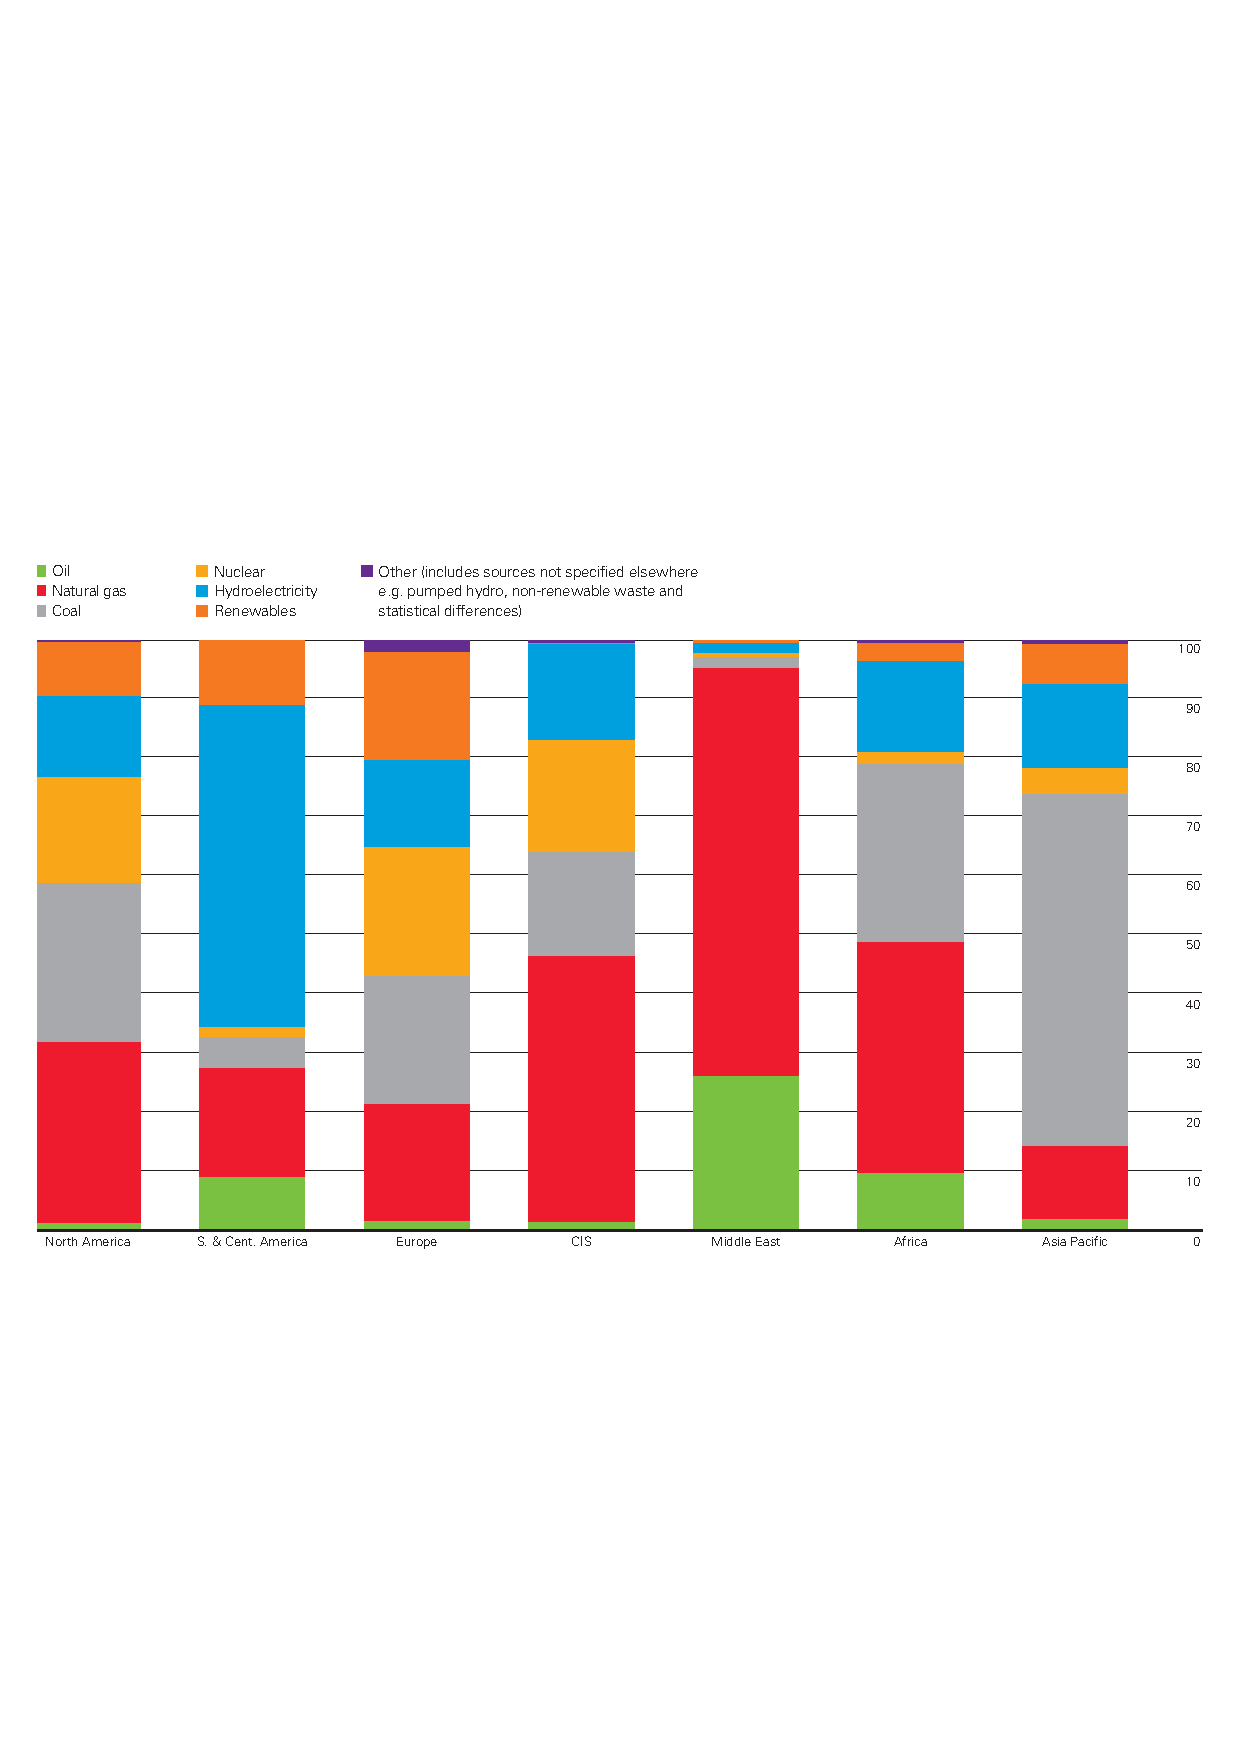
\includegraphics[width=\textwidth]{\figpath/Fig_cap_introduction/Energy_by_continent_2}
	\end{minipage}
		\begin{minipage}{.50\textwidth}
		(b) \\
		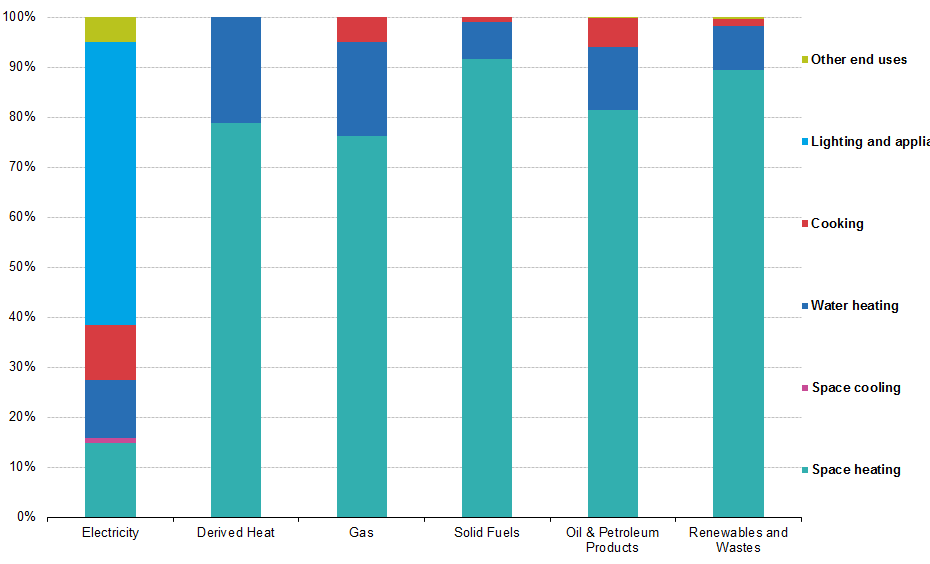
\includegraphics[width=\textwidth]{\figpath/Fig_cap_introduction/Energy-residential-EU}
	\end{minipage}
	\caption{(a) Electricity generation by different energy sources in 2017 by different continent by \cite{dudley2018bp}. (b) Energy use repartition in a residential buildings in Europe by \cite{dudley2018bp}.}
	 \label{fig-Energ-cons}
\end{center}	
\end{figure}

\noindent Research on environment-friendly energy sources, such as biomass, wind or solar have attracted many considerations recently.
Even though solar or wind energy are now operational, their main drawback remains the gap between their availability and the consumers demand.
Solar energy is not available during the nights for example, while wind energy is intermittent over the year.
The energy demand varies with time and the energy suppliers have to meet this demand.

\noindent Current solution to deal with this discrepancies of availability and demands problem is the use of energy storage systems.
The idea is to store the available energy at one time in one form or another and release it latter for a particular need, since energy availability and demand rarely concur.
The energy storage process is a crucial point for renewable and sustainable energy.
The later can be divided into five classes:
magnetic, biological, chemical, mechanical and thermal energy storages.
The main feature of the aforementioned energy storage technologies relies on energy charging and discharging process.
In most cases however, thermal energy is the energy form widely used.
Even the electricity generation is monitored by heat generating high temperature and high pressure.
Storing thermal energy is hence an efficient and fundamental way to store the energy.
It can be realised by rising the substance's temperature (sensible heat energy storage) or by changing the substance's phases (latent heat energy storage).


\begin{table}[!h]
	\begin{center}
		\begin{tabular}{ccccc}
			Agriculture & Buildings & Industry  & Transportation & Other  \\ \hline
			4.5 & 41.8 & 26 & 43.8 & 4.5 \\
		\end{tabular}
	\end{center}
	\caption {The energy consumed by different domain in France in 2017, in million tonne of oil equivalent. French ministry of ecological transition \citep{ministereEcologie2018}.}
	\label{tab-french-min}
\end{table}

\noindent To this end, research on passive heat storage system have attracted many considerations lastly, namely interest on Phase Change Material (PCM) as a latent heat energy storage have arisen.
PCM are used to store heat during the melting of the materials and releases later the stored energy during the solidification process.
At present, the latent heat storage technologies are proven as an effective solution to decrease the use of fossil fuel and in the same time increase the energy usage efficiency.


Aside from energy storage technologies, PCMs are also widely used in building applications, to decrease the temperature fluctuations.
Latest announcement of the french ministry of ecological transition, detailing the repartition of the energy consumption in different domains, indicates more than $35 \%$ of the total energy being consumed by residentials and commercial buildings. Details about energy consumptions in 2017, reported by the french ministry of ecological transition are shown in Tab. \ref{tab-french-min}.
More than $60\%$ of the total energy consumption in residential sector is dedicated to space heating (see Fig. \ref{fig-Energ-cons}b).
Research towards energy-efficient building to reduce heating and cooling demand is of principal interest nowadays.
Taking advantage of the high value of the latent heat of solid-liquid transformations, PCMs are extensively encountered in buildings thermal regulation to reduce overheating.
In summer, PCMs are used to absorb the excessive solar radiation heat and maintain a bracing indoor ambience.
PCM with a temperature of fusion close to the ambient temperature is generally used to ensure melting during the daytime and solidification during the nighttime.
During winter however, PCMs can be used to store heat generated by electrical heating system during the night and then release it in the daytime.

%The use of efficient insulation is the key of energy conservation in residential buildings.

\begin{table}[!h]
	\begin{flushleft}
		\begin{tabularx}{\linewidth}{cXX}
					Temperature range & PCM & Target application area \\ \hline \hline
			0 - 65 $^o C$ &    Paraffins (-3 to 64 $^o C$), water / ice  (0 $^o C$), stearic acide  (41 - 43 $^o C$), {n-octadecane  (27.7 $^o C$)}   &   Storage for domestic heating/cooling. Passive storage in bio-climatic building/architecture. Thermal storage of solar energy. Application in off-peak electricity for cooling and heating. Protection of electrical devices.\\ \hline
			%80 - 120 $^o C$ & Erythritol (117.7 $^o C$), RT100  (99 $^o C$),  $MgCl_2 6H_2 O$& \\ \hline
			80 - 120 $^o C$ &    Erythritol (117.7 $^o C$), RT100  (99 $^o C$), $MgCl_2 \, 6H_2O$  (116.7 $^o C$)   &   Storage for the hot-side of $LiBr/H_2O$ absorption cooling system with generator temperature requirements of less than 120 $^o$C\\ \hline
			$ > 150 $ $^o C$ &    $NaNO_3$ (310 $^o C$), $KNO_3$  (330 $^o C$), $NaOH$  (318 $^o C$),  $KOH$  (380 $^o C$), $ZnCl_2$  (280 $^o C$)  &   Storage for solar power plants based on parabolic trough collectors and direct steam generation.\\ 

		\end{tabularx}
	\end{flushleft}
	\caption {Target application area for some PCM studied in the literature \citep{agyenim2010review}.}
	\label{tab-PCM-app}
\end{table}

PCMs are a very timely subject and is encountered in a wide range of applications ranging from metal casting and passive temperature control devices (e.g. for modern portable electronics), to food freezing and cryosurgery.
In many of these applications, the choice of an appropriate material for a specific end depends of many criteria, such as the operating temperature range, the thermal conductivity, the costs, etc.
They are generally classified into three classes: organic, inorganic and eutectic.
A target application area for some PCM is drawn in Tab. \ref{tab-PCM-app}.
The main operating temperature range can be assorted by three groups. First, $0$ to $65 ^o C$ for thermal storage used in domestic heating/cooling or for thermal storage of solar energy. Paraffins and water are used for such applications.
Second, $80$ to $120 ^o C$ for the cooling of systems with generator temperature of less than $120 ^o C$ purpose.
Finally, greater than $150 ^o C$ for the heat storage in solar power plants based on parabolic trough collectors and direct steam generation.
For more details about these applications see \citep{agyenim2010review}.

Melting and solidification are also fundamental process in geophysical problem such as Earth's mantle formations, lava lakes \citep{davaille1993thermal}, thermal convection in magma chambers \citep{brandeis1989convective} or ice-melt lakes \citep{polashenski2012mechanisms}. Ice-melt ponds that form during summer season in the Arctic are known for example to display natural convection coupled to a phase-change process on the bottom side \citep{polashenski2012mechanisms,esfahani2018basal}. 
In that case, Rayleigh-B�nard like convection cells are observed in the liquid phase.

The solid-liquid phase-change phenomenon is a very complex process. 
It couples the natural convection in the liquid phase induced by the buoyancy force, the non-linear evolution of the phase-change interface and the heat transfer process, which could be different from one configuration to another.
The coupling of all these physical phenomenons induces strong non-linear process in the solid-liquid problems, difficult to analyse except for simple and ideal test cases.
Fig. \ref{fig:expe-PCM_Gong} showing the experimental investigation of the melting of n-octadecane inside a transparent brick by \cite{gong2015numerical} displays very well the complexity of the problem.
The investigated material is heated from the right and melts from the right to the left.
Figs. \ref{fig:expe-PCM_Gong}a and \ref{fig:expe-PCM_Gong}b indicate the evolution of the liquid fraction and the vector field in the fluid obtained by particle image velocimetry (PIV) method.
Capturing accurately the non-linear evolution of the solid-liquid interface, due to the strong convection in the melting PCM, is clearly a challenging numerical task.
Furthermore, the existence of boundary layers near the walls and the interface suggests that the mesh resolution should allow to capture these structures.

\begin{figure}[!h]
	\begin{center}
		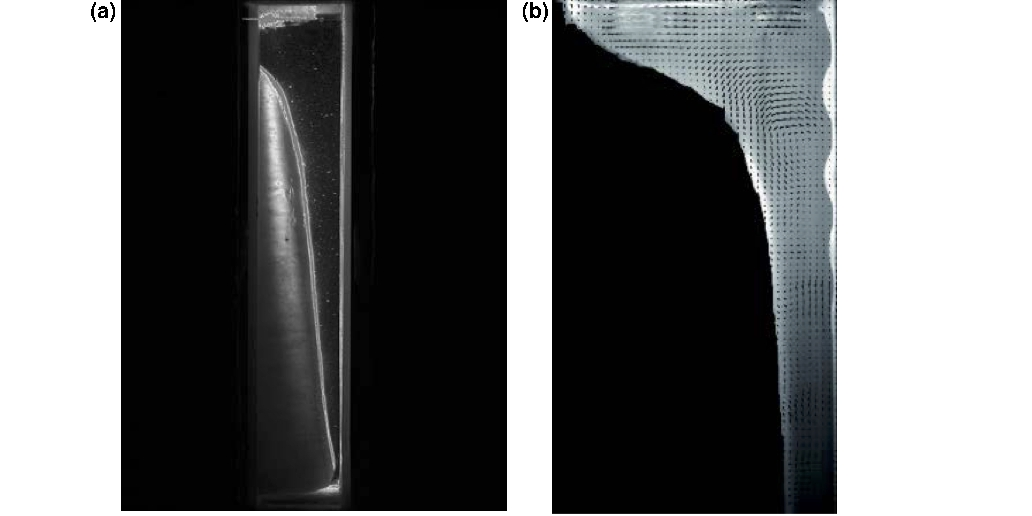
\includegraphics[width=\textwidth]{\figpath/Fig_cap_melting/EXPE_GONG_melting}
	\end{center}
	\caption{Experimental observation of the melting of n-octadecane within a transparent brick of plexiglas heated vertically from the left by \cite{gong2015numerical}, obtained by particle image velocimetry (PIV) method.}
	\label{fig:expe-PCM_Gong}
\end{figure}

Over the past $30$ years, solid-liquid phase-change has been widely studied. % using either numerical, analytical, or experimental methods.
Rectangular and cylindrical geometries were the most investigated configuration.
\cite{Okada1984,gau1983flow,gong2015numerical} have investigated experimentally the melting of n-octadecane and gallium PCMs inside rectangular containers.
\cite{ho1984inward,liu2014experimental,omojaro2017study} have studied experimentally the melting of different paraffin within cylindrical enclosures.
These experimental investigations have been extensively used for numerical validations (see \cite{bertrand1999melting,gobin2000melting,wang2010numerical,dan-2014-JCP,rakotondrandisa2019numerical}) and have permitted a better comprehension of the physical phenomenon that occurs during melting and solidification, mainly the heat transfer process.
%The experimental results are very often formulated in the form of mathematical correlations.
Experimental work of \cite{Okada1984} have permitted for example to express correlations of the variation of dimensionless thermal energy stored as latent heat, and the average Nusselt number on the vertical wall with the dimensionless time.
Later, \cite{ho1984inward} have analyzed the solid-liquid interface position for different configuration and \cite{jany1988scaling} have formulated $N\!u$-$\Ray$ correlation through a scaling analysis.
\cite{bejan1989analysis} gathered the previous observations and described analytically the solid-liquid melting process in the frame of vertical heating.

Gallium and n-octadecane are the most investigated materials. Experimentals \citep{gau1983flow,Okada1984,campbell1994visualization,gong2015numerical}, numericals \citep{rady1996natural,bertrand1999melting,hannoun2003resolving,Wang2010,dan-2014-JCP,rakotondrandisa2019numerical}, and theoreticals \citep{Okada1984,jany1988scaling,bejan1989analysis,kowalewski2004phase} works were  performed. 
Besides their physical properties are equal in both liquid and solid phases (differences less than $3 \%$), gallium and n-octadecane melt near room temperature, making them the preferred materials for experimentally investigating melting and solidification of low and high Prandtl-number PCMs respectively.
%These problems in a rectangular cavity have been also extensively used in the literature for the assessment of phase-change numerical methods

The previously mentioned works were mostly focused on studying separately melting or solidification problems
and only recently for alternate melting and solidification complete cycles \citep{wang2010numerical,rakotondrandisa2019numerical}. 
Prior to these studies on complete cycles, periodic melting and solidification problems were the most studied in the literature. 
\cite{ho1993periodic} and \cite{voller1996cyclic} studied numerically, periodic melting in square enclosures. 
Recently, \cite{hosseini2014experimental} carried out melting and solidification of a cylindrical PCM during charging and discharging process and \cite{chabot2017solid} studied analytically the effect of an alternate heating and cooling in a cylindrical PCM, with periodical boundary conditions.
We have also contributed recently on the comprehension of the governing mechanism during the melting and the solidification process in the paper \cite{rakotondrandisa2019numerical}.
We analysed in detail the difference between solidification occuring after a partial melting and a complete melting by providing temporal evolution of solid-liquid interface, liquid fraction, Nusselt number and accumulated heat input. 

While publication about melting and solidification of PCM heated from the side is very abundant, research on melting of PCM heated from below is quite rare.
\cite{diaz1984visualization,hale1980solid} have studied experimentally the solid-liquid interface morphology of PCM during basal heating.
\cite{gong1998flow} studied numerically the flow and heat transfer during the melting of pure n-octadecane in a rectangular cavity heated from below.
Recent numerical simulations have investigated different boundary conditions such as
periodic configurations along the horizontal axis \citep{esfahani2018basal,madruga2018dynamic,favier2019rayleigh} or wavy surface in a rectangular cavity heated from below \citep{kousksou2014melting}.
With regard to theoretical works, \cite{vasil2011dynamic,favier2019rayleigh} have studied the hydrodynamic instabilities at the onset of convection and compared their observation with the classical Rayleigh-B�nard instability mechanism \citep{chandrasekhar2013hydrodynamic}.
\cite{favier2019rayleigh} have focused their attention to the effect of the non-planar topography of the interface to the convection flow.
 On the other hand, \cite{gong1998flow,esfahani2018basal,madruga2018dynamic} mostly focused on global quantities such as the heat flux and the statistical properties of the interface.


\section{Purpose of the thesis}
The purpose of the present work is to investigate numerically solid-liquid phase-change systems.
The investigation tool used in this thesis is the open-source software FreeFem++ \citep{freefem,hecht-2012-JNM}.
A high accuracy numerical model using a Newton method with an adaptive finite element is used to simulate phase-change problems involving natural convection.

\noindent A first investigation on the numerical simulation of convective phase-change problems using adaptive finite element method have been carried out by \cite{dan-2014-JCP}.
The method used consists of solving the Navier-Stokes-Boussinesq equations by the mean of single domain approach using first order scheme.
The technique of variable viscosity approach was applied to annihilate the velocity in the solid phase.
The study was focused on two-dimensional square cavity configuration.

A first objective of this thesis is to improve the existing code, developed by the numerical methods and applications group of the LMRS Laboratory \footnote{http://lmrs-num.math.cnrs.fr}, and to organize the program as a toolbox for the software FreeFem++.
To this end, the objectives are listed as follows: 
\begin{enumerate}[label=(\roman*)]
\item increase the accuracy by using  a second order scheme for the time discretization and P$_2$ finite element for the temperature, 
\item implement a Carman-Kozeny model, in addition to the viscosity-based approach, to annihilate the velocity in the solid region, 
\item investigate challenging cases by simulating complex geometries (highly distorted mesh, cylindrical PCM with inner heated tubes) and computationally demanding cases (high Rayleigh numbers), 
\item simulate the complete melting-solidification cycle of a PCM. 
\end{enumerate}
A second objective is to extend the program to three-dimensional configurations.
The two dimensional assumption is indeed no more valid for high Rayleigh problems, especially for basal melting cases.
Moreover, three dimensional adaptive finite element method for convective melting problem is less investigated in the literature.

A third objective is to provide a thorough analysis of both melting and solidification process using the developed tools.

\newpage
\subsection{Existing method for modeling phase-change materials}
%Solid-liquid phase-change problems are encountered in numerous practical applications, ranging from metal casting and thermal energy storage (phase-change materials) to food freezing and cryosurgery. Melting and solidification are also fundamental processes in geophysical problems, such as Earth's mantle formation, lava lakes or magma chambers. 

Temperature gradients induce buoyancy forces in the liquid (melted) phase and generate a significant convective flow.
The appropriate mathematical description of the liquid phase is thus the usual model for the natural convection flow: the incompressible Navier-Stokes system of equations  with Boussinesq approximation for thermal (buoyancy) effects (\eg \cite{viskanta1985natural}). 
In this model, the energy conservation equation is written as a convection-diffusion equation for the temperature. 
In the solid phase, conduction is the main phenomenon and the appropriate model is the classical heat equation. 
The main modelling difficulty is to link these two models by taking into account the separation of the two phases by a sharp interface, across which thermodynamic properties are discontinuous. 

We offer in this section a description of the two main approaches suggested in the literature to deal with solid-liquid phase change problem.  
For a comprehensive review of models for phase-change problems with convection, see \cite{kowalewski2004phase}.  Note that a different category of models was recently suggested in the literature, based on the Lattice Boltzmann Method \citep{luo2015lattice,gong2015numerical} or meshless methods \cite{atluri2002meshless}.  Such methods based on non-deterministic models are not discussed in this introduction.

A first modelling  approach, usually referred to as the multi-domain (or deforming-grid) method, is based on the classical Stefan two-phase model. Solid and liquid domains are separated and the corresponding conservation equations are solved in each domain. Boundary conditions at the interface between domains are obtained by imposing the Stefan condition (balance  of heat fluxes at the interface). The position of the solid-liquid interface  is tracked and moved explicitly using  either {\em front tracking} or  {\em front fixing} methods. The  former method uses deforming grids to reconstruct the interface, while the latter is based on a time-depending coordinate transform, mapping the physical domain into a fixed computational domain. For a detailed description of these methods, see \eg \cite{sparrow1977analysis,unverdi-JCP-1992,gupta2000moving,Tenchev2005}. The main drawback of deforming-grid methods is their algorithmic complexity, which makes difficult to accurately capture solid-liquid interfaces of complicated shape or structure (\eg with mushy regions between solid and liquid phases). Configurations with multiple interacting interfaces (see the solidification of a phase-change material presented in this work) are also difficult to simulate with these methods (see also \cite{kowalewski2004phase-stella}). 

The second modelling approach avoids to impose explicitly the Stefan condition at the solid-liquid interface and therefore uses a single-domain (or fixed-grid) model. The same system of equations is solved in both liquid and solid phases. The energy balance at the interface is implicitly taken into account by the model. Consequently, the position of the interface is obtained a posteriori by post-processing the computed temperature field. Phase-field methods \citep{fabbri-JCP-1997} and enthalpy methods \citep{Voller-1987,Cao1989} are the most commonly used single-domain models. In phase-field methods, a supplementary partial differential equation for the evolution of the order parameter (a continuous variable taking the value 0 in the solid and 1 in the liquid) has to be solved, coupled with the conservation laws \citep{shyy-1996}. This new equation is model dependent and its numerical solution could lead to diffuse solid-liquid interfaces.  For recent contributions in this area, see \cite{boettinger2002phase,singer2008phase,favier2019rayleigh}. We focus below on enthalpy methods, which are the most widely used single-domain models due to their algorithmic simplicity. 

\noindent The main idea behind enthalpy models is to formulate the energy conservation law in terms of enthalpy and temperature and include latent heat effects in the definition of the enthalpy. The obtained equation applies to both liquid and solid phases and implicitly takes into account the separation of the phases. Another advantage of enthalpy methods, when compared to previously described models, is to  remove the limitation of the phase-change occurring at a fixed temperature. The presence of mushy regions can be easily modelled  with these methods. Two types of formulations of enthalpy methods exist in the literature, depending on the main variable used to solve the energy equation: enthalpy or temperature-based methods. \\
In enthalpy-based formulations  the main variable is the enthalpy \citep{eyres1946calculation,rose1960method,bhattacharya2014enthalpy}.  Temperature is computed  from the temperature-enthalpy coupling model. An iterative loop is necessary to solve the energy equation, formulated with both enthalpy and temperature variables. For a review of different iterative techniques to solve the energy equation, see \cite{Voller-1996-chapter}.  A second variety of enthalpy-based formulations consists in rewriting the energy equation with enthalpy terms only \citep{rady1996natural,hannoun2003resolving}. \\
In temperature-based formulations, the energy equation is formulated in terms of temperature only. The latent heat is  treated either by deriving an apparent heat capacity coefficient to define the total enthalpy \citep{Morgan-1978,chiesa1974natural,gau1984melting}  or by introducing a source term in the energy equation \citep{Voller-1996-chapter,swaminathan1997towards}. Advantages and drawbacks of each approach are discussed in detail in \cite{konig2017comprehensive}.

Single-domain methods are very appealing for numerical implementations. The same system of equations is solved in the entire computational domain, making possible algorithmic or computer-architecture optimisations. If enthalpy models offer an elegant solution to deal with the same energy conservation equation in both phases, a last modelling problem has to be solved. It concerns the  extension of the  Navier-Stokes-Boussinesq equations from the  liquid to the solid phase. 
Different techniques to bring the velocity to zero in the solid region were suggested. 

\noindent The most straightforward is the switch-off technique, which decouples solid and liquid computational points and overwrites the value of the velocity by setting it to zero in the solid region. Different implementations of this technique with finite-volume methods are presented in \cite{Ma2006,Wang2010}. 

\noindent In variable viscosity techniques \citep{gartling-1980,voller1987pcm,Cao1990}, the fluid viscosity depends on the temperature and is artificially increased to huge values in the solid regions through a regularisation or mushy zone. To avoid blow-up or numerical inconsistencies, the large gradients of viscosity must be correctly resolved in the mushy region.  
This is naturally achieved in finite-element methods with dynamical mesh adaptivity   \citep{dan-2014-JCP}, while in finite-volume methods with fixed grids, the time step has to be adapted to the space resolution \citep{Ma2006}. Versions of the variable viscosity approach suggested in  \cite{dan-2014-JCP} were further studied by \cite{aldbaissy2018full,WOODFIELD-2019} and implemented in a different finite-element framework (FEniCS) by \cite{zimmerman-2018}.

\noindent A third technique used to ensure a zero velocity field in the solid phase is the so-called enthalpy-porosity model \citep{Brent-1988}.  A penalisation source term is introduced in the momentum equation to allow the switch from the full Navier-Stokes equations in the liquid phase to a Darcy equation for porous media. The mushy region is thus regarded as a very dense porous medium that sharply brings the velocity to zero in the solid region. The expression of the penalisation source term generally follows the Carman-Kozeny model for the permeability of  a porous medium \citep{hannoun2003resolving,hannoun2005,Belhamadia2012}, but other mathematically equivalent expressions were suggested \citep{Angot-1999,favier2019rayleigh}. Different formulations and implementations of the enthalpy-porosity model are presented in \cite{Kowalewski-1999,Giangi-2000,kowalewski2004phase-stella}.

Concerning the space discretization of these models, finite difference (FD) or finite volume (FV) methods are generally used in the literature. 
When single-mesh models are used, the general strategy to capture the solid-liquid interface is to dramatically increase the mesh resolution in the whole domain. 
This results in a considerable increase of the computational time, even for two dimensional cases. 
 \citep{hannoun2003resolving} have reported that the simulation of the melting of tin within $200 \times 200$ fixed grid  required $2,400$ CPU hours, $111$ runs (restarts), and $3$ months of calculations.
Dynamical mesh adaptivity becomes in this context a valuable tool  to concentrate the grid refinement effort only in regions displaying high gradients of the computed variables (melting-solidification fronts, thermal or viscous boundary layers, recirculation zones). 

\noindent Finite  element (FE) methods offer this possibility to dynamically refine the mesh only in specific regions of the domain. %where sharp phenomena takes place (\eg solid-liquid interface, recirculation zones). 
Different FE approaches were suggested, from enthalpy-type methods (\eg \cite{elliott1987error}) to front-tracking methods (\eg \cite{CHLi}). 
Recently, adaptive FE methods were proposed for classical two-phase Stefan problem \citep{Belhamadia2004_S} using an anisotropic mesh adaptation algorithm based on solution-dependent metrics.
The authors extended  their algorithm for the three-dimensional simulation of the same problem  \citep{Belhamadia2004_3D} and showed that the use of locally adapted meshes with strong anisotropy proved to be very effective in reducing the number of computational nodes for such phase-change systems without convection.

\noindent To simulate melting or solidification problems with convection,  \cite{dan-2014-JCP}  recently suggested a dynamical mesh adaptation algorithm based on metrics control and implemented with the \ff software \citep{freefem,hecht-2012-JNM}. 
%and phase-change systems with convection  \citep{Belhamadia2012,dan-2014-JCP}. 
%For the classical two-phase Stefan problem, \cite{Belhamadia2004_S} suggested  an anisotropic mesh adaptation algorithm based on solution-dependent metrics. 
The advantage of this adaptive finite-element method, which will be also used in the present study, is to make possible, with reasonable computational cost, the re-meshing of the computational domain at each time step. 
A very refined discretization of the  regularization zone between solid and liquid phases is thus obtained, while regions with low gradients are de-refined in order to balance the overall computational effort. 

\subsection{Present numerical approach for modeling phase-change materials}
The present work is based on a single-domain enthalpy-porosity model for solid-liquid phase change problems with convection. 
For the energy conservation equation, a temperature-based formulation takes into account the latent heat by introducing  a discontinuous source term. 
For the mass and momentum conservation equations, we solve in the entire domain the incompressible Navier-Stokes equations with Boussinesq approximation for buoyancy effects. 
To bring the velocity to zero in the solid phase, we introduce in the momentum equation a penalty term following the Carman-Kozeny model.  
The coupled system of momentum and energy equations is integrated in time using a second-order Gear scheme. 
All the terms are treated implicitly and the resulting discretized equations are solved using a Newton method \citep{dan-2014-JCP}. 

\noindent The advantage of this formulation is to  permit a straightforward implementation of different types of non-linearities.
For the space discretization we use Taylor-Hood triangular finite elements, \ie P$_2$ for the velocity and P$_1$ for the pressure. 
Temperature is discretized using P$_2$ or P$_1$ finite elements. 
Discontinuous variables (latent heat, thermal diffusivity, etc) at the solid-liquid interface are regularized through an intermediate artificial mushy region.

\noindent Single domain methods require a refined mesh near the interface, where large enthalpy gradients have to be correctly resolved. 
An optimized dynamical mesh adaptivity algorithm allows us to adapt the mesh every time step and thus accurately capture the evolution of the interface.  
Mesh adaptivity, feature of the current method, offers the possibility to deal with complicated phase-change cases, involving multiple solid-liquid interfaces.

\noindent There are three main novelties in the present numerical approach, when compared to  \cite{dan-2014-JCP}: 
\begin{enumerate}[label=(\roman*)]
\item we use the Carman-Kozeny model to bring the velocity to zero inside the solid phase, instead of a  viscosity penalty method (imposing a large value of the viscosity in the solid), 
\item we increase  the time accuracy of the algorithm by replacing the first-order Euler scheme with the second-order Gear (BDF2) scheme (see also \cite{Belhamadia2012}), 
\item we improve the metric calculation procedure for mesh adaptivity.
\end{enumerate}

The programs were built and organized as a toolbox for \ff \citep{hecht-2012-JNM,freefem}, which is a free software (under LGPL license). \ff\footnote{\ff for different OS can be downloaded from \texttt{http://www3.freefem.org/}.} offers a large variety of triangular finite elements  (linear and quadratic Lagrangian elements, discontinuous P$_1$, Raviart-Thomas elements, etc.)  to solve partial differential equations. It is an integrated product with its own high level programming language and a syntax close to mathematical formulations, making the implementation of numerical algorithms very easy. Among the features making \ff an easy-to-use and highly adaptive  software we recall the advanced automatic mesh generator, mesh adaptation, problem description by its variational formulation, automatic interpolation of data, colour display on line, postscript printouts, etc. The \ff programming framework offers the advantage to hide all technical issues related to the implementation of the finite element method. It becomes then easy to  use the present toolbox to code new numerical algorithms for similar problems with phase-change.

%In this thesis, we use an enthalpy method with a temperature-based formulation using heat source term approach to simulate phase-change systems with convection.
%The natural convection flow in the liquid phase is simulated by solving the full incompressible Navier-Stokes equations with Boussinesq approximation.
%A Carman-Kozeny type penalty model is applied to ensure a zero velocity value in the solid region.
%The main feature of our numerical approach is the use of an adaptive finite element method to accurately track the solid-liquid interface.
%Single domain method requires actually a fine mesh near the phase change front in order to capture the large enthalpy gradient. 
%The smaller the phase change interval the narrower the mushy region and the more refined the mesh should be.
%Yet applying a fine mesh in the whole domain would increase considerably the computational time.
%Hence, we introduce a FE method with time-dependent mesh adaptivity by metric control that is  effective for a large range of phase-change systems with convection, from melting to solidification. The proposed mesh refinement strategy has the capacity to take into account different metrics and thus the ability to refine the mesh in different regions of interest in the computational domain. In particular, we show that the method is able to simultaneously track several interfaces in the domain.\\ 
%The nonlinear system of equations are solved by means of a Newton algorithm.
%A fully-implicit Newton method for the phase-change system based on a finite-element formulation of the Navier-Stokes equations has been derived by \citep{dan-2014-JCP}.
%The advantage of this formulation is to  permit a straightforward implementation of different types of non-linearities in the system of equations.
%
% The code was built as a toolbox for FreeFem++ \citep{hecht-2012-JNM,freefem}, which is a free software (under LGPL license) using a large variety of triangular finite elements  (linear and quadratic Lagrangian elements, discontinuous P$_1$, Raviart-Thomas elements, etc.)  to solve partial differential equations. FreeFem++ is an integrated product with its own high level programming language and a syntax close to mathematical formulations, making the implementation of numerical algorithms very easy. Among the features making FreeFem++ an easy-to-use and highly adaptive  software we recall the advanced automatic mesh generator, mesh adaptation, problem description by its variational formulation, automatic interpolation of data, colour display on line, postscript printouts, etc. FreeFem++ community is continuously growing, with  thousands of users all over the world.

\section{Thesis plan}
Chapter \ref{chap-NSB} sets the mathematical and physical basis of the numerical system used to simulate phase-change problems involving natural convection flow.
We present in detail the incompressible Navier-Stokes-Boussinesq equation and the single-domain approach to solve the same system of equations throughout the whole domain.
The enthalpy method, modeling the phase-change phenomenon is presented first.
The Navier-Stokes equation with Boussinesq approximation to simulate the natural convection in the liquid flow is then developed.
Finally, the final non-dimensional system of equations is described in detail with a discussion about the Carman-Kozeny model used as a penalty term in the momentum equation.

Chapter \ref{chap-FEM} is devoted to the numerical algorithm for solving the numerical system presented previously.
The finite element algorithm we have developed in this work is first presented in detail: time integration scheme, finite element discretization and the Newton method.
The characteristics Galerkin method, an alternative for the treatment of non-linear term in the momentum equation, is also presented.
Then, we describe the mesh adaptivity by metric control, which is a standard function offered by FreeFem++.
Some theoretical tests to assess for the accuracy of our numerical method is also presented.
The space and the time convergence orders are demonstrated using the Burggraf flow and a manufactured solution designed for the incompressible Navier-Stokes equation.
The structure of the new finite-element toolbox for the simulation of PCMs is also described.
The program architecture and the parameter details are presented.
Finally, the domain decomposition method used for large scale simulation is described.

A first validation of our numerical method is addressed in Chapter \ref{chap-NATCONV}.
The capability of the code to deal with linear and non-linear forms of the buoyancy force in the Boussinesq approximation is first tested.
%Differentially heated cavity (horizontal $\nabla T$) configuration is used to compare our results with benchmarks solution existing in the literature.
The test cases are presented by increasing progressively the difficulty.
We simulate first the natural convection of air in square enclosures differentially heated from the vertical walls.
Then heated obstacle is added in the center of the domain.
Finally, we add non-linearity by simulating the natural convection of water.
%Three-dimensional simulations of the natural convection of air is also presented.
%For both two and three-dimensional configurations, qualitative and quantitative validations are provided.

Once the capability of our algorithm to deal with natural convection issues was demonstrated, much more attention to phase-change problem is paid.
Numerical simulation of melting and solidification of PCM is considered in Chapter \ref{chap-MELTING}.
The melting of octadecane and gallium inside rectangular enclosures are investigated first since they were extensively used for numerical method validations, because of their physical properties relatively equal in both solid and liquid phases.
Finally, several PCM container geometries are simulated to prove the robustness of our numerical method, mainly cylindrical and irregular domain are computed.
%Finally, numerical simulation of three-dimensional configuration is presented.

Numerical and scale analysis are investigated in Chapter \ref{chap-MELTING-ANALYSIS}.
We compare the behavior of the PCM when lateral and basal heating are of interest.
The melting of octadecane heated from the side is carried out first.
Then numerical results for the melting from below is performed.
For  both cases, we provide detailed description of the melting process with scaling analysis to better understanding the heat transfer mechanism.
%Accurate comparison is carried out for the differentially heated cavity case, by considering different size of the cavity and different temperature difference between the hot temperature and the temperature of fusion, which are the main parameters monitoring the natural convection in the melting PCM.
Analysis of the time evolution of some physical parameters, such as the Nusselt number, the liquid fraction, the accumulated heat input and the time evolution of the melting are discussed. %provided in detail through a scaling analysis.

Chapter \ref{chap-SOLIDIFICATION} displays the numerical simulation of a full cycle melting/solidification of a PCM. 
Two solidification fronts have to be tracked and make the case very challenging.
A differentially heated cavity case and a circular PCM with inner heated tubes are studied.
A comparison on the influence of the Rayleigh number during the melting and the solidification process is emphasized, since both cycles are not driven by the same mechanism.

Chapter \ref{chap-3D-SIMULATION} is devoted for three-dimensional configurations simulated using parallel algorithm.
3D simulations of PCM are indeed less investigated in the literature.

Finally, Chapter \ref{chap-conclusion} draws the conclusion of this study and some perspectives for future developments.



%%%%%%%%%%%%%%%%%%don't forget if needed %%%%%%%%%%%%%%%%%%%%%
%\section[toc version]{title version%
%              \sectionmark{head version}}
%\sectionmark{head version}
%%%%%%%%%%%%%%%%%%%%%%%%%%%%%%%%%%%%%%%%%%%%%%%%%%%%%%%%%%%%%%
\def\titcourt{Navier-Stokes-Boussinesq model and Enthalpy method}
\def\titlong{Navier-Stokes-Boussinesq model and Ethalpy method}
%%%%%%%%%%%%%%%%%%%%%%%%%%%%%%%%%%%%%%%%%%%%%%%%%%%%%%%%%%%%%%%%
\chapter[\titlong]{\titlong%
              \chaptermark{\titcourt}}
\chaptermark{\titcourt}
\label{chap-NSB}
%%%%%%%%%%%%%%%%%%%%%%%%%%%%%%%%%%%%%%%%%%%%%%%%%%%%%%%%%%%%%%%%
%%%%%%%%%%%%%%%%%%%%%%%%%%%%%%%%%%%%%%%%%%%%%%%%%%%%%%%%%%%%%%%%

%\section{Governing equations} \label{sec-gov-eq}
%%%%%%%%%%%%%%%%%%%%%%%%%%%%

We consider a solid-liquid system placed in a two-dimensional numerical domain of characteristic length $L_{ref}$. 
In the following, subscripts $s$ and $l$ will refer to the solid and liquid phases, respectively. 

The single domain approach, using the same system of equations in both phases is described first in detail.
%For the numerical implementation, it is convenient to adopt a single-domain approach to describe both phases using the same system of equations. 
The model is based on the Navier-Stokes equations with Boussinesq approximation, which is the natural description of the fluid flow with natural convection. 
A penalty term is added to the momentum equations to bring the velocity to zero inside the solid region. 
For the energy conservation equation, an enthalpy method is used to model the phase change process. %The single-domain model is  in detail in the following sections.
Secondly, a scale analysis is presented in order to have a comprehensive view of the melting and the heat transfer rate during the phase-change.

\section{Enthalpy method}

The phase change process is modeled using an enthalpy method \citep{voller1987pcm,Cao1989,Cao1990} with temperature-based formulation. We start from the energy equation:
\begin{equation}
\label{eq-energie}
   \frac{\partial (\rho h)}{\partial t_{\varphi}} + \nabla \cdot(\rho h \vec{\tilde{u}}) - \nabla \cdot (k \nabla T) = 0,
\end{equation}
where $t_{\varphi}$ is the physical time, $h$ the enthalpy, $\rho$ the density, $\vec{\tilde{u}}$  the velocity vector, $T$ the temperature and $k$ the thermal conductivity. 
To make eq. (\ref{eq-energie})  valid for the entire domain containing both liquid and solid phases, the total enthalpy $h$ is regarded as the sum of the sensible heat and the latent heat:
\begin{equation}
\label{eq-enth-model}
  h = c ( T + s(T) ),
\end{equation} 
with $c$ the local specific heat. The function $s(T)$ is introduced to model the jump of the enthalpy due to the phase change and is theoretically a Heaviside step function depending on the temperature: it takes the zero value in the solid region and a large value in the liquid, equal to $h_{sl}/c$, with $h_{sl}$ the latent heat of fusion. 
Linear  \citep{voller1987pcm,Wang2010} or smoother functions \citep{dan-2014-JCP} can be used to regularize $s(T)$ and also the jump of material properties (from solid to liquid). 
We use a regularization of all step-type functions by a continuous and differentiable hyperbolic-tangent function suggested by \cite{dan-2014-JCP} (see below). 
\Blue{%Moreover, we assume that the undercooling problem is here negligible since only pure and homogeneous materials are considered.
We assume moreover that the undercooling phenomenon is negligible (see also \cite{wang2010numerical,kowalewski2004phase}).}

Eq. (\ref{eq-energie}) can be further simplified by considering the following assumptions: (i) the density difference between solid and liquid phases is negligible, \ie $\rho_l=\rho_s=\rho$ is constant. 
We note however that this is not strictly true for all substances, but also serves as a convenient simplification; (ii) the regularization zone is narrow and the velocity inside this zone is very low. 
Consequently, the final expression of the energy equation is obtained by combining eqs. (\ref{eq-enth-model})  and (\ref{eq-energie}) and  neglecting the convection term $\nabla \cdot ( c s \vec{\tilde{u}})$\footnote{In the liquid phase, $\nabla \cdot ( c s \vec{\tilde{u}})  = h_{sl} \nabla \cdot  \vec{\tilde{u}}=0$; in the solid phase, $s=0$; in the regularization region, it is assumed that $\vec{\tilde{u}}=0.$}:
\begin{equation}\label{eq-energie-enth-model}
\frac{\partial \left(c T\right)}{\partial t_{\varphi}} + \nabla \cdot\left( c T \vec{\tilde{u}}\right) -
\nabla \cdot\left( \frac{k}{\rho} \nabla T \right) +  \frac{\partial \left(c s\right)}{\partial t_{\varphi}}  = 0.
\end{equation}
The essential feature of the current approach is that the phase change front is not tracked explicitly but is instead recovered a posteriori from the computed temperature field.
The phase-change occurs over a temperature interval $  T \in [T_f - T_{\varepsilon1}, T_f + T_{\varepsilon2}] $ around the temperature of fusion $T_f$.
For non-isothermal phase-change PCM, $T_{\varepsilon1}$ and $T_{\varepsilon2}$ correspond to the solidus and the liquidus temperature of the material.
However, for a pure material involving a unique phase-change temperature, $T_{\varepsilon1}$ and $T_{\varepsilon2}$ represent an artificial mushy zone used to regularize discontinuous parameters and should be set as small as possible.
The solid-liquid interface is thus identified through the isoline $T=T_f$.
One could include the Gibbs-Thomson effect due to the surface energy of the solid-liquid interface which is assumed to be negligible in our simulations.

\section{Navier-Stokes equations with Boussinesq approximation}

The natural convection in the liquid part of the system is modeled using the incompressible Navier-Stokes equations, with  Boussinesq approximation for buoyancy effects. To make this model valid for both liquid and solid phases, the momentum equation is modified as follows:
\begin{equation}\label{eq-momentum-conserv-1}
  \rho \left( \frac{\partial \vec{\tilde{u}}}{\partial t_{\varphi}} +   {(\vec{\tilde{u}}\cdot\nabla ) \vec{\tilde{u}}} \right) + \nabla P - \mu_{l}  {\nabla^2 \vec{\tilde{u}}} 
+ \rho g \vec{e}_y= A(T) \vec{\tilde{u}},
\end{equation}
where$P$ denotes the pressure, $\mu_{l}$ the dynamic viscosity of the liquid (assumed to be constant).  
%and $f_B(T)$ the Boussinesq force. 

The penalty term $A(T) \vec{\tilde{u}}$ is artificially introduced in eq. (\ref{eq-momentum-conserv-1}) to extend this equation in the solid phase, where the velocity, pressure, viscosity and Boussinesq force are meaningless.  Consequently, $A(T)$  is modelled to vanish in the liquid, where the Navier-Stokes-Boussinesq momentum equation is recovered. A large value of $A(T)$ is imposed in the solid, reducing the momentum eq. (\ref{eq-momentum-conserv-1})  to $A(T) \vec{\tilde{u}}=0$, equivalent to $\vec{\tilde{u}}=0$. Exact expression for $A$ will be given in the next section.

The density is assumed to be constant everywhere except in the body force term $\rho g$ of the $\vec e_y$ momentum eq. (\ref{eq-momentum-conserv-1}).
Under the assumption of a small variation of the density and the temperature, the Boussinesq approximation allows to linearize the density as follows:
\begin{equation}
   \rho = \rho_{ref} (1 - \beta (T-T_{ref})),
\end{equation}
with $\beta = - (1/\rho_{ref}) (\partial \rho / \partial T)$ the thermal expansion coefficient and $(\rho_{ref},T_{ref})$ a reference states.
It is worth noting that this approximation is valid for $\beta (T - T_{ref})$ considerably smaller than unity.
Therefore, the momentum equation can be written as:

\begin{equation}\label{eq-momentum-conserv}
  \frac{\partial \vec{\tilde{u}}}{\partial t_{\varphi}} +   {(\vec{\tilde{u}}\cdot\nabla ) \vec{\tilde{u}}} + \nabla p - \nu_{l}  {\nabla^2 \vec{\tilde{u}}} 
- f_B(T) \vec{e}_y= A(T) \vec{\tilde{u}},
\end{equation}
where  $\nu_l = \mu_l/\rho$ is the kinematic viscosity,  $p = (P + \rho_{ref} g y)/ \rho_{ref}$ accounting for the hydrostatic pressure $\rho_{ref} g y$ and $f_B(T) = g \beta (T-T_{ref})$ denotes the buoyancy force.

Finally, the conservation of mass in the liquid phase is expressed by the continuity equation in the frame of incompressible fluid:
\begin{equation}\label{eq-mass-conserv}
\nabla \cdot \vec{\tilde{u}} = 0.
\end{equation} 

The final system of equations for the single-domain approach is thus:
\begin{eqnarray}
	\nabla \cdot \vec{\tilde{u}} &=& 0, \\
	\frac{\partial \vec{\tilde{u}}}{\partial t_{\varphi}} +   {(\vec{\tilde{u}}\cdot\nabla ) \vec{\tilde{u}}} + \nabla p - \nu_{l}  {\nabla^2 \vec{\tilde{u}}} 
- f_B(T) \vec{e}_y - A(T) \vec{\tilde{u}} & = & 0, \\
	\frac{\partial \left(c T\right)}{\partial t_{\varphi}} + \nabla \cdot\left( c T \vec{\tilde{u}}\right) -
\nabla \cdot\left( \frac{k}{\rho} \nabla T \right) +  \frac{\partial \left(c s\right)}{\partial t_{\varphi}}  &=& 0.
\end{eqnarray}


\section{Dimensionless system of equations for the single-domain approach}\label{sec-eq-scaling}

It is convenient to numerically solve a dimensionless form of the previous equations.
Using the length scale $L_{ref}$ and a reference state $(\rho, V_{ref}, T_{ref})$, we can define the following scaling for the space, velocity, temperature and time variables:
\begin{equation}\label{eq-adim}
\vec{x} = \frac{\vec{\tilde{x}}}{L_{ref}} \, , \,  \vec{u} = \frac{\vec{\tilde{u}}}{V_{ref}} \, , \,  \theta = \frac{T-T_{ref}}{\delta T} \, , \,  t = \frac{V_{ref}}{L_{ref}} \, t_{\varphi},
\end{equation}
Temperatures $T_h$ (hot) and $T_c$ (cold) will be used to set isothermal boundary conditions. The difference $\delta T$, 
%$\delta T=T_{h}-T_{f}$with $T_f$ the temperature of fusion, 
is considered as the representative temperature scale  for the natural convection onset in the liquid region. 
For the classical natural convection problem without phase-change, $\delta T$ could be defined as $\delta T=T_{h}-T_{c}$ since the flow in the fluid is driven by the temperature difference between the "hot" and the "cold" temperature.
However, for the melting PCM, the convection is driven by the temperature difference $\delta T=T_{h}-T_{f}$, with $T_f$ the temperature of fusion.
As far as the solidification process is concerned, a distinct discussion will be provided in sec. (\ref{chap-SOLIDIFICATION}). % during the melting,  and $\delta T = T_f - T_c$ during the solidification. }
Thus $\delta T$ is used to define the Rayleigh number of the flow:
\begin{equation}
\label{eq-Rayleigh}
\Ray = \frac{g \beta L_{ref}^3 \delta T}{\nu_l \alpha_l},
\end{equation}
where $\alpha = k/(\rho c)$ is the thermal diffusivity. 
Note that the reference temperature for the phase-change problem is   $T_f$, resulting in  $\theta_f = 0$.
Since the mushy zone is defined for  $  \theta_f - \varepsilon_1 \, \leq \theta \leq \, \theta_f + \varepsilon_2 $, this choice of the reference temperature 
simplifies the identification of the latter to  $  -\varepsilon_1 \, \leq \theta \leq \,\varepsilon_2 $.
The solid-liquid interface is therefore identified by the isoline $\theta=0$.

Finally, the dimensionless system of equations to be solved in both liquid and solid regions can be written as:
\begin{eqnarray}
\nabla\cdot \vec{u}&=&0, \label{eq-qmvt} \\ \vspace{0.2cm}
 \frac{\partial \vec{u}}{\partial t} + {(\vec{u}\cdot\nabla) \vec{u}} +\nabla p -\frac{1}{\Rey}{\nabla^2 \vec{u}} 
 - f_B(\theta)\, \vec{e}_y - A(\theta) \vec{u}&=&0, \label{eq-qmvt-2} \\ \vspace{0.2cm}
 \frac{\partial \left(C \theta\right)}{\partial t} + \nabla \cdot\left( C \theta \vec{u}\right) -
 \nabla \cdot\left( \frac{K}{\Rey \Pr} \nabla \theta \right) +  \frac{\partial \left(C S\right)}{\partial t}  &=& 0, \label{eq-energ} 
\end{eqnarray}
where the linearised (Boussinesq) buoyancy force ($f_B$), the Reynolds ($\Rey$) and Prandtl ($\Pr$) numbers are defined as:
\begin{equation}\label{eq-RePr}
f_B(\theta) = \frac{\Ray}{\Pr \Rey^2} \theta, \quad \Rey = \frac{\rho V_{ref} L_{ref}}{\mu_l}=  \frac{V_{ref} L_{ref}}{\nu_l} , \quad \Pr = \frac{\nu_l}{\alpha_l}.
\end{equation}
Non-dimensional conductivity and specific heat are functions of the temperature $\theta$, 
\begin{equation}\label{eq-adimKC}
K(\theta)= \frac{k}{k_l} , \,  \, C(\theta) = \frac{c}{c_l},
\end{equation}
and have to take into account the variation of material properties between the solid and the liquid regions. 

In the energy eq. (\ref{eq-energ}), the non-dimensional function $S = s/\delta T$, introduced by the enthalpy model, is regularized across the mushy region using a hyperbolic-tangent function \citep{dan-2014-JCP}:
\begin{equation}
S(\theta) = S_{l} + \frac{S_{s}-S_{l}}{2}\left\{
1 + \tanh\left(\frac{\theta_r-\theta}{R_r}\right)
\right\},
\label{eq-Stanh}
\end{equation} 
where $\theta_r$ is the central value around which we regularize (typically $\theta_r=\theta_f=0$) and $R_r$ the smoothing radius (typically $R_r=\varepsilon$). Note that $S_{s} = 0$ and
\begin{equation}
S_{l} = \frac{h_{sl}/c_l}{\delta T} = \frac{1}{\Ste},
\label{eq-Ste}
\end{equation} 
where $Ste$ is the Stefan number. Regularizations similar to eq. (\ref{eq-Stanh}) are used to model the variation inside the regularization region of functions (\ref{eq-adimKC}) defining material properties.
We note that linear functions \citep{voller1987pcm,wang2010numerical} or cubic Hermite polynomial \citep{Belhamadia2012} are also used in the literature.

Finally, the penalty term in the momentum eq. (\ref{eq-qmvt-2}) is derived from the Darcy's law, by modeling the fluid flow within the mushy region as a flow through a porous medium.
In fact, the Darcy's law states that the velocity of flow in porous medium is proportional to the pressure gradient:

\begin{equation}
	\vec u = - \frac{\zeta^*}{\mu} \vec \nabla p.
\end{equation}
where $\zeta^*$ is the permeability, which is a function of the porosity.
As the porosity decreases, the permeability (and the velocity) also decreases, down to the limiting value of zero when the mush becomes completely solid.
This behavior can be accounted in a numerical model by adding a source term $A \vec u$ in the momentum equation.
The well-known equation derived from the Darcy law, the Carman-Kozeny eq.\ref{ck eq}, could be a suitable form for the function $A$:

\begin{equation} \label{ck eq}
	\nabla p = - \frac{\CKC (1 - \lambda)^2}{\lambda^3} \vec u.
\end{equation}

Finally $A$ takes the form \citep{Belhamadia2012,kheirabadi2015effect}:

\begin{equation}\label{eq-CK}
A(\theta) = -\frac{\CKC (1 - \varphi(\theta))^2}{\varphi(\theta)^3 + b},
\end{equation}
where $\varphi(\theta)$ is the phase-change variable, which is  $1$ in the fluid region and $0$ in the solid. Inside the regularization region,  $\varphi(\theta)$ is regularized using a hyperbolic-tangent function similar to eq. (\ref{eq-Stanh}).
The constant $\CKC$ is set to a  large value (as discussed below) and  the constant $b=10^{-6}$ is introduced to avoid division by zero.

\section{Boundary layer approximation and scale analysis}
Either PCM is used for energy storage or for building insulation or for other purposes, one would necessarily assess the heat transfer during the phase-change process.
Mainly, it was extensively proven that the convective heat transfer plays significant role during the melting stage.
Therefore, before solving numerically eqs. (\ref{eq-qmvt}) - (\ref{eq-energ}), we first rely on scale analysis to predict theoretically the fluid flow and heat transfer patterns that can develop in the fluid part.
The idea behind the scaling analysis is about identifying the proper scales of the phenomenon, in order to understand the evolution of the heat transfer and the melting rates.

In the present analysis, we will consider first only the liquid phase without phase-change.
A further analysis of the scale during the melting will be developed in sec. (\ref{chap-MELTING-CAVITY}).
We consider a two-dimensional enclosure of height H filled with Newtonian fluid, differentially heated from the vertical walls and insulated from the horizontal walls.
A No-slip boundary condition is considered for the velocity. 
Since no external force is applied to our system, the fluid flow is merely driven by natural convection flow, induced by temperature differences from the vertical walls.
It is well-known from the foregoing boundary conditions that the fluid layer situated close to the vertical walls stuck to the wall and are motionless.
The heat transfer through the fluid layer immediately adjacent to the wall is accordingly by pure conduction, i.e, $ q = - \left. (\partial \theta/ \partial x) \right |_{x=0} $.
We therefore define the average Nusselt number to quantify the heat transfer rate at the heated wall:
\begin{equation}\label{eq-def-Nu}
   N\!u = - \int_0^1 \left. \frac{\partial \theta}{\partial x} \right |_{x=0} dy.
\end{equation}

When a steady state could be reached, the fluid near each sidewall is characterized by two boundary layers: a thermal boundary layer of thickness $\delta_{\theta}$ and a viscous boundary layer of thickness $\delta_\nu$.
The boundary layer approximation assumes that the flow and the energy transfer are restricted predominantly to the boundary layer region.
This theory was proposed first by Prandtl in 1904 and validated later by many experimental and numerical studies.
The main consequences of the boundary layer approximations are that: \\
{\it (i)} the normal part of the momentum equation has a negligible importance, \\
{\it (ii)} the downstream diffusion term in the momentum and energy equations are neglected in comparison with the normal diffusion terms ($\partial^2 \vec{u}/\partial y^2 \ll \partial^2 \vec{u}/\partial x^2$ and $\partial^2 T/\partial y^2 \ll \partial^2 T/\partial x^2$) since the boundary layer thickness is much smaller than the enclosure height ($ \delta \ll H$), \\
{\it (iii)} the pressure distribution is purely hydrostatic, i.e, $P = - \rho g y$, \\
{\it (iv)} the thermal and the viscous boundary layer thickness are given by the order of magnitude expressions: $\delta_\nu/\delta_\theta = o \left(\Pr^{1/2} \right)$.\\
These assumptions lead to the following boundary layer equations for the conservation of mass, momentum and energy:
\begin{eqnarray} \label{eq-bound-mass}
	\frac{\partial u}{\partial x} + \frac{\partial v}{\partial y} &=& 0, \\  \label{eq-bound-mom}
	u \frac{\partial v}{\partial x} + v \frac{\partial v}{\partial y} &=& \nu \frac{\partial^2 v}{\partial x^2} + g \beta (T - T_{ref}), \\ \label{eq-bound-energy}
	u \frac{\partial T}{\partial x} + v \frac{\partial T}{\partial y} &=& \alpha \frac{\partial^2 T}{\partial x^2}. 
\end{eqnarray}
The mass conservation in eq. (\ref{eq-bound-mass}) in the boundary layer region leads to:
\begin{equation}
	\frac{u}{\delta_\theta} \sim \frac{v}{H}.
\end{equation}
The energy eq. (\ref{eq-bound-energy}) expresses a balance between longitudinal convection and transverse conduction:
\begin{equation}
	\frac{v}{H} \sim \frac{\alpha}{\delta_\theta^2},
\end{equation}
which yields:
\begin{equation} \label{eq-scale-v}
	v \sim \frac{\alpha H}{\delta_\theta^2}.
\end{equation}
As far as momentum eq. (\ref{eq-bound-mom}) is concerned, we could identify the interplay among three forces:
\begin{equation} \label{eq-scale-momentum}
	\underbrace{\frac{v^2}{H}}_{inertia} \quad \underbrace{\nu \frac{v}{\delta_\theta^2}}_{friction} \quad \underbrace{g \beta \delta T}_{buoyancy}.
\end{equation}
Using the expression of $v$ in eq. (\ref{eq-scale-v}) and by dividing eq. (\ref{eq-scale-momentum}) by $g \beta \delta T$, we obtain:
\begin{equation} \label{eq-final-scale}
	\underbrace{\left( \frac{H}{\delta_\theta} \right)^4 Pr ^{-1} \Ray^{-1}}_{inertia} \quad  \underbrace{\left( \frac{H}{\delta_\theta} \right)^4 \Ray^{-1}}_{friction} \quad \underbrace{1}_{buoyancy}.
\end{equation}
Eq. (\ref{eq-final-scale}) indicates that the behaviour of the fluid in the boundary layer depends on the $\Pr$ number. \\
First, for a high-Prandtl fluid ($\Pr \geq 1$), the friction-buoyancy balance yields: 
\begin{equation}
	\delta_\theta \sim H \Ray^{-1/4}.
\end{equation}
The Nusselt number from eq. (\ref{eq-def-Nu}) scales as $H/\delta_\theta$, resulting: 
\begin{equation}
	N\!u \sim Ra^{1/4}
\end{equation}
and $v \sim \alpha/H \Ray^{1/2}$. \\
Second, for a low-Prandtl fluid ($\Pr \ll 1$), we observe a balance between inertia and buoyancy, leading to:
\begin{equation} \label{eq-corr-Low-Pr}
	\delta_\theta \sim H Pr^{-1/4} \Ray^{-1/4}.
\end{equation}
Accordingly we obtain a Nu-Ra correlation:
\begin{equation}
	Nu \sim Pr^{1/4} \Ray^{1/4}.
\end{equation}


%Let us consider eqs. (\ref{eq-qmvt}) - (\ref{eq-energ}) in the thermal boundary layer region ($x \sim \delta_\theta$, $y \sim H$), where the heating effect of the wall is maximum.


%The approximation commonly employed, in addition to the Boussinesq approximation, to analyse the behaviour of the heat transfer in the boundary layer is the boundary layer assumption.
%
%
%
%For further simplification, our analysis will be considered at the steady state, i.e reasonable Rayleigh number are of interests ($\Ray \leq 10^7$).
%Following the boundary layer approximation, the following assumptions could be taken.


\graphicspath{{\figpath/Fig_cap_2}}
%%%%%%%%%%%%%%%%%%don't forget if needed %%%%%%%%%%%%%%%%%%%%%
%\section[toc version]{title version%
%              \sectionmark{head version}}
%\sectionmark{head version}
%%%%%%%%%%%%%%%%%%%%%%%%%%%%%%%%%%%%%%%%%%%%%%%%%%%%%%%%%%%%%%
\def\titcourt{Finite element method}
\def\titlong{Finite element method for the Navier-Stokes-Boussinesq equations using Newton algorithm}
%%%%%%%%%%%%%%%%%%%%%%%%%%%%%%%%%%%%%%%%%%%%%%%%%%%%%%%%%%%%%%%%
\chapter[\titlong]{\titlong%
              \chaptermark{\titcourt}}
\chaptermark{\titcourt}
\label{chap-FEM}
%%%%%%%%%%%%%%%%%%%%%%%%%%%%%%%%%%%%%%%%%%%%%%%%%%%%%%%%%%%%%%%%
%%%%%%%%%%%%%%%%%%%%%%%%%%%%%%%%%%%%%%%%%%%%%%%%%%%%%%%%%%%%%%%%

%\section{Numerical method}\label{sec: num meth}

This chapter sets the numerical algorithm for solving the system of equation described previously in Chapter \ref{chap-NSB} for both two and three-dimensional configurations.
The finite element method and the Newton algorithm are presented first in detail.
%The accuracy of the developed method is then assessed with some basic theoretical test for two-dimensional configurations.
Then, the domain decomposition method for the three-dimensional configuration is discussed.% with a strong scalability analysis.

\section{Motivation for the choice of the numerical method}
%Aside from the non-linear convection terms in the momentum and the energy Eqs. \ref{eq-qmvt} - \ref{eq-energ}, a further difficulty arise from the non-linearity introduced by the source term $\partial (CS)/\partial t$ in Eq. \ref{eq-energ}.
In many in-house or commercial codes used to simulate phase-change problems (ANSYS CFX, Fluent, etc.),
finite difference (FD) or finite volume (FV) methods are used in most of the time with a fixed-mesh approach.
Accurate simulations are therefore carried out by increasing considerably the mesh resolution in the whole domain, increasing consequently dramatically the computational time.
At the example of \cite{voller1996cyclic} who used insufficient grid resolution to compute the melting of gallium, \cite{wang2010numerical} had to consider thinner mesh, resulting by a strong increase, of a factor of three, of the total mesh number to capture correctly the boundary layer structures. 

Our choice for the finite element (FE) methods is motivated by its capability to adapt dynamically the mesh and to deal with several geometrical domain.
The adaptive capabilities of FE discretization by applying finer mesh where sharp phenomena takes place (solid-liquid interfaces, boundary layers, recirculation zones, ...) and coarser mesh elsewhere (in the solid, in the bulk of the fluid region where the gradient are lower than the boundary layer region, ...) is helpful to reduce the degree of freedom involved in the numerical resolution and thus reduce the computational time.
We use a finite-element method that was implemented using the open-source software FreeFem++ \citep{freefem,hecht-2012-JNM}, using a large variety of triangular finite elements  to solve partial differential equations. 

FreeFem++  is an integrated product with its own high level programming language and a syntax close to mathematical formulations, making the implementation of numerical algorithms very easy. Among the numerous numerical tools offered by FreeFem++, the use of the powerful mesh adaptivity function proved mandatory in this study to obtain accurate results within reasonable computational time.
The numerical code was optimized to afford the mesh refinement every time step:  the mesh density was increased around  the phase change interfaces,  offering an optimal resolution of the large gradients of all regularized functions ($S, K, L_f$), while  the mesh was de-refined (larger triangles) in the solid part, where a coarser mesh could be used. A simulation using a globally refined mesh would require a prohibitive computational time for an equivalent accuracy of the melting front resolution. Similar algorithms based on FreeFem++  were successfully used for solving different systems of equations with locally sharp variation of the solution, such as Gross-Pitaevskii equation \citep{dan-2010-JCP,dan-2016-CPC} or  Laplace equations with nonlinear source terms \citep{dan-2013-AMM}. 

The space discretization is based on Taylor-Hood finite elements, approximating  the velocity with $P_{2}$ Lagrange finite elements (piecewise quadratic), and the
the pressure with the $P_{1}$ finite elements (piecewise linear). The temperature and the enthalpy are discretized using $P_2$ finite elements.  
This discretization is second order accurate in space.
We also use a second order accurate discretization in time.
\cite{aldbaissy2018full} have compared analytically and numerically the first and second order discretization of the time-dependent Boussinesq problem, and have concluded that the second order scheme is much better than the first order in terms of CPU time with the same precision.
A fully implicit backward second order scheme (BDF2 or GEAR) is employed in the present study. The time derivative of a variable $\phi$ is approximated  by:
\begin{equation}	
\label{eq-Gear}
	\frac{d\phi}{dt} \simeq \frac{3\phi^{n+1} - 4\phi^{n}+ \phi^{n-1}}{2\delta t},
\end{equation}

\noindent computing the solution $\phi^{n+1}$ at time  $t_{n+1}=(n+1) \delta t$ by using two previous states ($\phi^{n}, \phi^{n-1}$). We use this scheme to advance in time both velocity ($\phi=\vec{u}$) and temperature fields  ($\phi=\theta$).  The other terms in Eqs. \ref{eq-qmvt} - \ref{eq-energ} are treated implicitly (\ie taken at time $t_{n+1}$). The resulting non-linear equations are solved using a Newton algorithm. 

\noindent Some authors have used a Richardson extrapolation \citep{Belhamadia2012,wang2010numerical} in the momentum equation by extrapolating U from previous time steps.
We have tested this approach but the results exhibit less accurate solutions and the computations requests small $\delta t$.
In addition, a projection algorithm with an explicit discretization of the Navier-Stokes-Boussinesq equations was also investigated, using the Adams-Bashforth and Crank-Nicolson second order scheme.
The main drawback is the very small $\delta t$ ($\sim 10^{-6}$ vs $10^{-1}$ for the fully implicit discretization) needed to ensure convergence at each time steps.

\noindent A last alternative for the treatment of non-linear terms in the momentum equation is offered by the characteristics Galerkin method \cite{Pironneau92}.
This method will be discussed in detail in Sec. \ref{sec-charac-FreeFem}.

Finally, a supplementary difficulty comes from the one-domain method which need techniques to bring the velocity to zero in the solid region.
The switch-off technique, the variable viscosity approach and the Carman-Kozeny penalty term are the most used in the literature.
The physical meaning of the variable viscosity formulation and the Carman-Kozeny penalty term is fundamentally different.
The Carman-Kozeny approach considers the mushy zone as a porous media, i.e the solid is stationary and the liquid flows through the porous structures, 
while the variable viscosity formulation treats the mushy zone as a mixture of solid crystals and liquid, permitting thus a movement of both the solid and the liquid.
The $\mu$-based method was investigated by \cite{dan-2014-JCP} and the Carman-Kozeny penalty method is investigated in the present work.
We note however that techniques in FV methods based on the modification of the numerical algorithm by cutting-off the velocity in the solid by a relaxation scheme also exists.

\newpage
\section{Finite element algorithm} \label{sec-FE-algo}

To solve the system of Eqs. \ref{eq-qmvt} - \ref{eq-energ} we use a finite-element method that was implemented using the open-source software \ff \citep{freefem,hecht-2012-JNM}.
Finite-element methods for solving Navier-Stokes type systems of equations  are generally based on a separate discretization of the temporal derivative (using finite difference, splitting or characteristics methods) and the generalization of the Stokes problem for the resulting system \citep{Temam,GRaviart,Quarteroni}. 
We use the second-order implicit finite-difference discretization in Eq. \ref{eq-Gear} of the temporal derivative and obtain the time semi-discretization of the single-domain model (Eq. \ref{eq-qmvt} - \ref{eq-energ}):
\begin{eqnarray} \label{eq-time-disc1}
\nabla\cdot \vec{u}^{n+1} + {\gamma} p^{n+1} &=& 0, \\ %\nonumber
\frac{3}{2} \frac{\vec{u}^{n+1}}{\delta t} +(\vec{u}^{n+1}\cdot\nabla) \vec{u}^{n+1} +\nabla p^{n+1} 
- {\frac{1}{Re} \nabla^2 \vec u^{n+1}}  & & \\ \nonumber 
- A(\theta^{n+1})\vec u^{n+1}- f_B(\theta^{n+1}) \, \vec{e}_y &=&  \\ \nonumber
2 \frac{\vec{u}^{n}}{\delta t}-\frac{\vec{u}^{n-1}}{2\delta t},\\ \label{eq-time-disc3}
\frac{3}{2} \frac{\theta^{n+1} + S(\theta^{n+1})}{\delta t} +
\nabla\cdot\left(\vec{u}^{n+1} \theta^{n+1}\right)
- \nabla \cdot\left( \frac{K}{RePr} \nabla \theta^{n+1} \right) &=& \\  \nonumber
2\frac{ \theta^{n} + S(\theta^{n})}{\delta t}-\frac{ \theta^{n-1} + S(\theta^{n-1}) }{2\delta t}.
\end{eqnarray}

\noindent The penalty parameter $\gamma$ takes very low values ($\gamma=10^{-7}$)  to ensure a pressure field with zero average and, at the algebraic level, fulfill the diagonal of the pressure term.  
This system of non-linear equations is solved at time  $t_{n+1}=(n+1) \delta t$, using two  previous states at $t_{n}$ and $t_{n-1}$.

The space discretization of variables over the domain $\Omega=[0,1]^2$ uses a finite-element method based on a weak formulation of the system of Eqs. \ref{eq-time-disc1} - \ref{eq-time-disc3}. 
We consider homogeneous Dirichlet boundary conditions for the velocity, \ie $\vec{u}=0$ on $\pl \Omega$, and set the classical Hilbert spaces for the velocity and pressure:

\begin{equation}
\vec{V}=V\times V, \, V=H^1_0(\Omega), \quad Q=\left\{q\in L^2(\Omega)\left|\; \int_{\Omega}q=0\right.\right\}
\end{equation}

\noindent Following the generalization of the Stokes problem \citep{Temam,GRaviart,Quarteroni}, the variational formulation of the system  of Eqs. \ref{eq-time-disc1} - \ref{eq-time-disc3} can be written as: find $(\vec{u}^{n+1}, p^{n+1}, \theta^{n+1}) \in \vec{V}\times Q\times V$, such that
\begin{eqnarray}
\label{eq-weak-all}
b\left(\vec{u}^{n+1}, q\right) - \gamma (p^{n+1},q)&=& \\ \nonumber
0, \, \forall \, q \in Q \\ %\nonumber
\frac{3}{2 \delta t} \left(\vec{u}^{n+1},\vec{v}\right) + c\left(\vec{u}^{n+1} ; \vec{u}^{n+1}, \vec{v} \right) +
{a\left(\vec{u}^{n+1}, \vec{v}\right)} & &\\ \nonumber
- (A(\theta^{n+1}) \, \vec u^{n+1},\vec v)+ b\left(\vec{v}, p^{n+1}\right)
- {\left(f_B(\theta^{n+1}) \, \vec{e}_y,\vec{v}\right)}
&=& \\ \nonumber
\frac{2}{\delta t} \left(\vec{u}^{n},\vec{v}\right) 
- \frac{1}{2 \delta t} \left(\vec{u}^{n-1},\vec{v}\right), \, \forall \, \vec{v} \in \vec{V}\\ \label{eq-weak-energy}  %\nonumber
\frac{3}{2 \delta t} \left(\theta^{n+1} + S(\theta^{n+1}), \phi\right)
+\left(\vec{u}^{n+1} \cdot \nabla \theta^{n+1} , \phi
\right) +
\left( \frac{K}{Re Pr} \nabla \theta^{n+1}, \nabla \phi \right) &=& \\  \nonumber
\frac{2}{\delta t} \left( \theta^{n}+S(\theta^n), \phi\right)
- \frac{1}{2 \delta t} \left( \theta^{n-1}+S(\theta^{n-1}), \phi\right),\, \forall \, \phi \in V,
\end{eqnarray}

\noindent where {$(u , v)=\int_{\Omega} u\cdot v$} denotes the scalar product in $L^2(\Omega)$ or $\left(L^2(\Omega)\right)^2$; the bilinear forms $a, b$ and trilinear form $c$ are defined as \cite{GRaviart,Quarteroni}:

\begingroup{ \small
	\begin{eqnarray*}\nonumber
		a: \vec{V} \times \vec{V} \rightarrow \R, & & a(\vec{u},\vec{v})= \int_{\Omega}  
			 \vec{\nabla^t} \vec{u} : \vec{\nabla} \vec{v} = \sum_{i,j=1}^2 \int_{\Omega}   \pl_j u_j \cdot \pl_j v_i,\\ 
		b: \vec{V} \times Q \rightarrow \R, & & b(\vec{u},q) = -\int_{\Omega}\nabla \cdot\vec{u}\, q =
		-\sum_{i=1}^2\int_{\Omega}\pl_i u_i\cdot q, \\ \nonumber
		c: \vec{V} \times \vec{V} \times \vec{V} \rightarrow \R, & & c(\vec{w}; \vec{z}, \vec{v})=\int_{\Omega} \left[\left(\vec{w} \cdot \nabla\right) \vec{z}\right] \cdot\vec{v}
		=\sum_{i,j=1}^2\int_{\Omega} w_j (\pl_j z_i) v_i.
		\label{eq-biforms}
	\end{eqnarray*}
}


The system of non-linear Eqs. \ref{eq-weak-all} - \ref{eq-weak-energy} is solved using a Newton method. To advance the solution from time $t_n$ to $t_{n+1}$, we start from an initial guess $w_0 = (\vec{u}^{n}, p^{n}, \theta^{n})$ (which is the solution at $t_n$), and construct the Newton sequence $w_k = (u_k, p_k, \theta_k)$ by solving for each inner iteration $k$:

\begin{equation}
D_w{\cal F} (w_k ) w_{k+1} = D_w{\cal F}(w_k) w_k -  {\cal F}(w_k).
\label{eq-newton-w}
\end{equation}

\noindent $D_w{\cal F}$ is the linear operator representing the differential of $\cal F$.
Eq. \ref{eq-newton-w} can be rewritten as follow when applied to the discretized equation, in which Eqs. \ref{eq-weak-all} - \ref{eq-weak-energy} are regarded as ${\cal F}(w) = 0$:

\begingroup \small{
	\begin{eqnarray} \label{eq-newton-C1}
	b\left(\vec{u}_{k+1}, q\right) - \gamma (p_{k+1},q) &=& 0, \\ \label{eq-newton-C2}%\nonumber
	\frac{3}{2 \delta t} \left(\vec{u}_{k+1},\vec{v}\right) 
	+ c\left(\vec{u}_{k+1} ; \vec{u}_{k}, \vec{v} \right)
	&+& c\left(\vec{u}_{k} ; \vec{u}_{k+1}, \vec{v} \right)\\ \nonumber
	+ 
	\frac{1}{Re} a\left( \vec{u}_{k+1}, \vec{v}\right)
	- \left(\frac{d A}{d\theta}(\theta_k)\, \theta_{k+1} \, \vec{u}_k, \vec{v}\right) 
	&-& \left(A(\theta_k) \, \vec{u}_{k+1}, \vec{v}\right) + b\left(\vec{v}, p_{k+1}\right)  \\  \nonumber
	- {\left(\frac{df_B}{d\theta}(\theta_k)\, \theta_{k+1} \, \vec{e}_y, \vec{v}\right)} &=&  
	\frac{1}{\delta t} \left( 2 \vec{u}^n - \frac{1}{2} \vec{u}^{n-1},\vec{v}\right) \\ \nonumber
	+ c\left(\vec{u}_k ; \vec{u}_{k}, \vec{v} \right) - \left(\frac{d A}{d\theta}(\theta_k)\, \theta_{k} \, \vec{u}_k, \vec{v}\right)
	&-& \left( \left(\frac{df_B}{d\theta}(\theta_k)\, \theta_{k} - f_B(\theta_k)\right)\, \vec{e}_y,\vec{v}\right), \,\,\, \\   %\nonumber
	\frac{3}{2\delta t} \left(\theta_{k+1} + \frac{dS}{d\theta}(\theta_k)\, \theta_{k+1}, \phi\right)
	+\left(\vec{u}_{k} \cdot \nabla \theta_{k+1} , \phi  \right)
	&+& \left( \vec{u}_{k+1} \cdot \nabla  \theta_k , \phi \right) \\ \nonumber
	+ \left( \frac{K}{Re Pr} \nabla \theta_{k+1}, \nabla \phi \right) 
	&=&
	\frac{2}{\delta t} \left(\theta^n + S(\theta^n) , \phi\right)  \\ \label{eq-newton-C3} \nonumber
	+\left(\vec{u}_{k} \cdot \nabla  \theta_k, \phi \right)
	+ \frac{3}{2 \delta t} \left(\frac{dS}{d\theta}(\theta_k)\, \theta_{k}  - S(\theta_k),\, \phi\right) 
	&-& \frac{1}{2 \delta t} \left(\theta^{n-1} + S(\theta^{n-1}),\, \phi\right).\,\,\,
	\end{eqnarray}
} \endgroup

\noindent Note that the last term of Eq. \ref{eq-newton-C2} cancels in the case of a linear Boussinesq force $f_B$  (see Eq. \ref{eq-RePr}); this is not the case when non-linear variations of the density of the liquid are considered (convection or solidification of water).  Note also that the previous system of Eqs. \ref{eq-newton-C1} - \ref{eq-newton-C3} depends only on $\vec{u}^n$, $\vec{u}^{n-1}$, $\theta^n$ and $\theta^{n-1}$ and is independent of $p^n$, the pressure being in this approach a Lagrange multiplier for the divergence free constraint. 
We underline the fact that the Newton loop (following $k$) has to be iterated until convergence for each time step $\delta t$ following the algorithm

\begin{equation} \label{eq-Newton-algo}
\begin{tabular}{||ll}
\multicolumn{2}{||l}{Navier-Stokes time loop following $n$}\\
\multicolumn{2}{||l}{set  $w_0=(\vec{u}^{n}, p^{n}, \theta^{n})$}\\
& \begin{tabular}[t]{||ll}
\multicolumn{2}{||l}{Newton iterations  following $k$}\\
&solve (\ref{eq-newton-C1}) to get $ \vec w_{k+1} $\\
\multicolumn{2}{||l}{stop when  $\| \vec w_{k+1} - \vec w_k \| < \xi_N$}
\end{tabular}\\
\multicolumn{2}{||l}{actualize $(\vec{u}^{n+1}, p^{n+1}, \theta^{n+1}) = w_{k+1}$}
\end{tabular}
\end{equation}

\noindent In some cases, it is more relevant to solve directly the steady equation corresponding to Eqs. \ref{eq-weak-all} - \ref{eq-weak-energy} (i.e. without the temporal derivatives), when a steady state could be achieved.
It is for example the case for natural convection of air or water in differentially heated configurations.
In that case, the weak formulation of the problem becomes:

\begin{eqnarray}
\label{eq-weak-steady}
b\left(\vec{u}^{n+1}, q\right) - \gamma (p^{n+1},q)&=& 0, \\ %\nonumber
\left(\vec{u}^{n+1},\vec{v}\right) + c\left(\vec{u}^{n+1} ; \vec{u}^{n+1}, \vec{v} \right) +
{a\left(\vec{u}^{n+1}, \vec{v}\right)} & & \\ \nonumber
- (A(\theta^{n+1}) \, \vec u^{n+1},\vec v)+ b\left(\vec{v}, p^{n+1}\right)
-  \underline{\Red{\alpha} {\left(f_B(\theta^{n+1}) \, \vec{e}_y,\vec{v}\right)}}
&=& 0, \\ \label{eq-weak-energy-steady}  %\nonumber
\left(\vec{u}^{n+1} \cdot \nabla \theta^{n+1} , \phi
\right) +
\left( \frac{K}{Re Pr} \nabla \theta^{n+1}, \nabla \phi \right) &=& %\\  \nonumber
0,
\end{eqnarray}

\noindent The parameter $\alpha$ is introduced before the buoyancy force term $f_B$ as a convergence parameter of the Newton algorithm.
The initial condition should be indeed close to the solution to limit the Newton iteration and ensure the convergence of the method.
The idea is to solve successive steady problems by increasing $\alpha$ from $0$ to $1$.
At each stage, the previous computed solution is set as initial conditions.
These steps could be assimilate to a smooth increase of the $\Ray$ number,

\begin{equation} \label{eq-Newton-steady}
\begin{tabular}{||ll}
\multicolumn{2}{||l}{Loops for $m$ steps}\\
\multicolumn{2}{||l}{set  $w_0=(\vec{u}^{n}, p^{n}, \theta^{n})$}\\
& \begin{tabular}[t]{||ll}
\multicolumn{2}{||l}{Newton iterations  following $k$}\\
&solve Eq. \ref{eq-weak-steady} - \ref{eq-weak-energy-steady} with $\alpha = \left( \frac{m}{\mathcal{N}} \right)^4$\\
\multicolumn{2}{||l}{stop when  $\| \vec w_{k+1} - \vec w_k \| < \xi_N$}
\end{tabular}\\
\multicolumn{2}{||l}{actualize $(\vec{u}^{n+1}, p^{n+1}, \theta^{n+1}) = w_{k+1}$}
\end{tabular}
\end{equation}

\noindent with $\mathcal{N}$ the number of steps.

\noindent This approach allows to achieve the natural convection of air in $6$ iterations for $\Ray = 10^6$ instead of $150$ iterations when the unsteady system of equations is solved.

\newpage
\section{Characteristics method for the convective terms} \label{sec-charac-FreeFem}

An alternative for the treatment of non-linear terms in the momentum equation is offered by the characteristics Galerkin method \cite{Pironneau92}. Defining the characteristic flow (passing at time $t$ through the point $\vec{x}$)
\begin{equation}
\left\{
\begin{array}{l}\vspace{0.2cm}
\ds\frac{\partial \vec{X} }{\partial \tau}(\tau, t, \vec{x})=\vec{u} (\tau,\vec{X} (\tau,t, \vec{x})), \quad \tau\in (0,t_{max})\\
\vec{X} (t, t, \vec{x}) = \vec{x},
\end{array}
\right.
\label{eq-charactD}
\end{equation}
one can express the substantial (total) derivative of any function $\Phi(t,\vec{x})$ as
\begin{equation}
\frac{D\Phi}{Dt}(t,\vec{x})=\left( \frac{\partial \Phi}{\partial
	t}+\vec{u}\cdot\nabla \Phi \right)(t,\vec{x})=\frac{\partial}{\partial
	t}\left(\Phi(\tau, \vec{X}(\tau,t, \vec{x}))\right)|_{\tau=t},
\end{equation}
and finally use the time discretization:
\begin{equation}
\left(\frac{D\Phi}{Dt}\right)^{n+1}(\vec{x})\approx\frac{\Phi^{n+1}(\vec{x})-\Phi^{n}\circ \vec{X}^n(\vec{x})}{\delta t},
\end{equation}
with $\vec{X}^n(\vec{x})$ a suitable approximation of $\vec{X}(t_n,t_{n+1},\vec{x})$, obtained by an integration back in time of Eq. \ref{eq-charact} from $t_{n+1}$ to $t_n$ for each grid point $\vec{x}$. The Galerkin characteristic method is implemented in Freefem++ as an operator computing $\Phi \circ \vec{X}^n$ for given mesh, convection velocity field and time step.

\noindent The weak formulation in Eq. \ref{eq-weak-all} becomes after using the characteristics method:

\begin{eqnarray}
\label{eq-charact}
b\left(\vec{u}^{n+1}, q\right) - \gamma (p^{n+1},q)&=& \\ \nonumber
0, \, \forall \, q \in Q \\ \nonumber
\frac{3}{2 \delta t} \left(\vec{u}^{n+1},\vec{v}\right) +
a\left(\vec{u}^{n+1}, \vec{v}\right) 
+ b\left(\vec{v}, p^{n+1}\right) 
- f_B(\theta^{n+1}) \left(\vec{e}_y,\vec{v}\right)
&=& \\ \nonumber
\frac{2}{\delta t} \left(\vec{u}^{n}\circ \vec{X}^n,\vec{v}\right) - \frac{1}{2 \delta t} \left(\vec{u}^{n-1}\circ \vec{X}^{n-1},\vec{v}\right), \, \forall \, \vec{v} \in \vec{V}\\  \nonumber
\frac{3}{2 \delta t} \left(\theta^{n+1}, \phi\right)  
+
\left( \frac{K}{\Prd} \nabla \theta^{n+1}, \nabla \phi \right) &=& \\ \nonumber
 \frac{2}{\delta t} \left(\theta^{n}\circ \vec{X}^n, \phi\right) -  \frac{1}{2 \delta t} \left(\theta^{n-1}\circ \vec{X}^{n-1}, \phi\right), \, \forall \, \phi \in V,
\end{eqnarray}

\noindent The system of Eq. \ref{eq-charact} is then solved to advance the solution from $t_n$ to $t_{n+1}$ in one step. The drawback of the method is that it requires small time steps for accurately computing of the convection terms. 

%\newpage
 \section{Mesh adaptivity} \label{subs:FEadapt}
We use the standard mesh adaptivity function (\texttt{adaptmesh}) offered by \ff \citep{hecht-2012-JNM}. The key idea implemented in this function (see also \cite{hecht-1996-missi,hecht-2000-ijnmf,hecht-1997-aiaa,george-1998,frey-george-1999,moham-piron-2000})  is to modify the scalar product used in the automatic mesh generator to evaluate distance and volume.  Equilateral elements are thus constructed, accordingly to the new metric.  The scalar
product is based on the evaluation of the Hessian $\mathcal{H}$ of the variables of the problem. For example, for a P$_1$ discretization of a
variable $\chi$, the interpolation error is bounded by:
\begin{equation}
{\cal E } = |\chi - \Pi_h \chi |_0 \leq c \sup_{T\in \mathcal{T}_{h}} \sup_{x,y,z\in T}   |\mathcal{H}(x)|(y-z , y-z),
\label{eq1}
\end{equation}

\noindent where $\Pi_h \chi $ is the $P_1$ interpolate  of $\chi$, $ |\mathcal{H}(x)|$ is the  Hessian of $\chi$ at point $x$ after being made positive definite.
Using the Delaunay algorithm (\eg \cite{george-1998}) to generate a  triangular mesh with edges close to the unit length  in the metric  $\mathcal{M} ={|\mathcal{H}| \over (c {\cal{E}})}$ will result in a equally distributed  interpolation error ${\cal E}$ over the edges $a_i$ of the mesh. More precisely, we get
\begin{equation}
{1 \over c {\cal E}} a_i^T {\cal M } a_i \le 1.
\end{equation}


The previous approach could be generalized for a vector variable $\chi=[\chi_1, \chi_2]$. After computing the metrics $\mathcal{M}_{1}$ and $\mathcal{M}_{2}$ for each variable, we define a metric intersection  $\mathcal{M} = \mathcal{M}_{1} \cap \mathcal{M}_{2}$,
such that the unit ball of $\mathcal{M}$ is included in  the intersection of the two  unit balls  of metrics $\mathcal{M}_{2}$ and $\mathcal{M}_{1}$
(for details, see the  procedure defined in \cite{frey-george-1999}).

The \texttt{adaptmesh} function offers the possibility to take into account several metrics computed from different variables monitoring the evolution of the phase-change system. For natural convection system, the mesh will be adapted using the values of the two velocity components and the temperature. For phase-change systems, to accurately track the solid-liquid interface we add the variation of the enthalphy source term in the adaptivity criterion. For  water systems (convection or freezing), we also add an extra function tracking the anomalous change of density around $4 {^o}C$. To reduce the impact of the interpolation on the global accuracy for time-depending problems, we consider, for each variable used for adaptivity,  the metrics computed at actual ($t_{n+1}$) and  previous ($t_{n}$) time instants (see also \cite{Belhamadia2004_S}). The anisotropy of the mesh is a parameter of the algorithm and it was set to values close to 1. This is an inevitable limitation since we also impose the minimum edge-length of triangles to avoid too large meshes.
The capabilities of the mesh adaptivity algorithm are illustrated in Chapter \ref{chap-MELTING}.

\newpage
\section{A finite-element toolbox for the simulation of phase-change systems with natural convection}\label{sec-desc-prog}

The methods described previously were implemented in a 2D toolbox based on \ff software.
The \ff syntax to implement the Newton algorithm is very close to the mathematical formulation given above. \\
After defining a vectorial finite-element space \texttt{fespace Wh(Th,[P2,P2,P1,P1]);}, associated to the mesh \texttt{Th}, we define the velocity, pressure and temperature variables in a compact manner by \texttt{Wh [u1,u2,p,T];}. Corresponding test functions are defined similarly. It is then very easy to define a \texttt{problem} formulation in \ff and include all the terms of the algorithm in Eqs. \ref{eq-newton-C1} - \ref{eq-newton-C2}. This makes the lecture of the programs very intuitive by comparing each term to its mathematical expression. New terms could be added to the variational formulation expressed in the \texttt{problem} structure, without affecting other parts of the program. Consequently, the implementation of new models  or numerical methods for this problem is greatly facilitated by this modular structure of programs.
	
In this section we first describe the architecture of the programs and the organisation of files.
Then we focus on the list of input parameters and the structure of output files.
%
\begin{figure}
	\begin{center}
		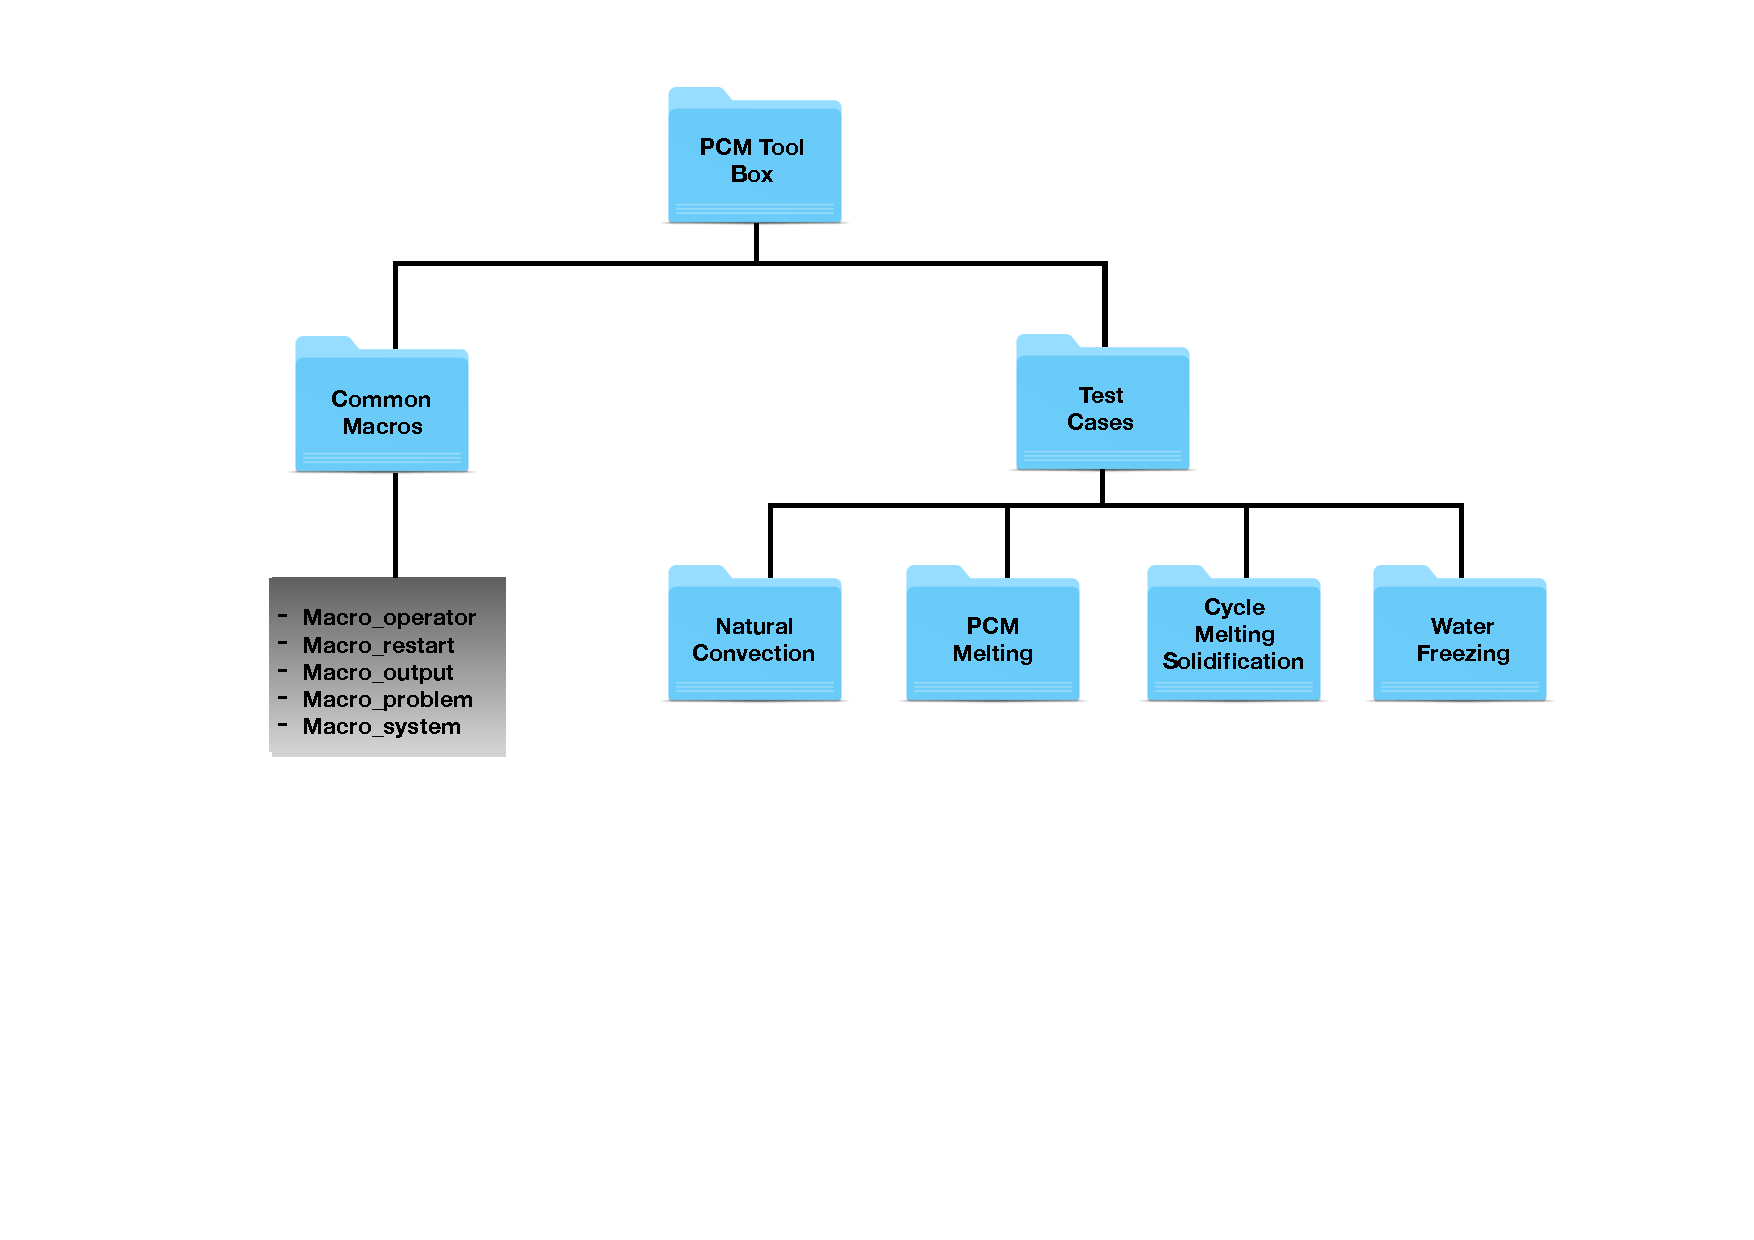
\includegraphics[width=0.9\textwidth]{\figpath/Fig_cap_2/FOLDER_arbor_3}
	\end{center}
	\caption{Folder tree structure of the FreeFem++ toolbox to solve phase change problems. Test cases and common macros are separated into two folders.}
	\label{fig-folder-tree}
\end{figure}

\subsection{Program architecture}
Fig. \ref{fig-folder-tree} gives a schematic overview of the content of the toolbox. All files are provided in a directory called \texttt{PCM-Toolbox}.  Many detailed comments are included in the programs, with direct link to the mathematical expressions used in this chapter. The used \ff syntax was intentionally kept at a low level of technicality and supplemented with detailed comments when specific more technical syntax was used.

\noindent This directory is organized as follows:
\begin{enumerate}
   \item The directory \texttt{Common-Macros} contains five files:\\
$\bullet$ {\em Macro$\_$operator.idp} includes macros and functions defining mathematical operators,\\
$\bullet$ {\em Macro$\_$problem.idp}: macros defining the variational formulation of the problem,\\
$\bullet$ {\em Macro$\_$restart.idp}: macros used to start a new simulation from a saved field,\\
$\bullet$ {\em Macro$\_$output.idp}: macros used to save the solution with different formats,\\
$\bullet$ {\em Macro$\_$system.idp}: macros identifying the OS and defining specific OS-commands.

   \item The directory \texttt{Test-Cases}  contains four subdirectories, each of them defining one of the following applications:\\
    $\bullet$  natural convection of air or water in a differentially heated square cavity, \\
    $\bullet$  melting of a PCM stored in containers of different shapes,\\
    $\bullet$  melting followed by solidification of a rectangular PCM,\\
    $\bullet$  freezing of pure water in a square cavity.
    
   \noindent Each subdirectory contains  three files: {\em NEWTON$\_$\$case.edp} is the main \ff script file, $param_\_phys.inc$ defines the physical parameters and $param_\_num.inc$ the numerical parameters. For example, to run the natural convection case of air in a square cavity, the user can use the following command in a terminal window:
  \texttt{FreeFem++ NEWTON$\_$stat$\_$natconv.edp}.
  
  \noindent The folder structure of each test case is illustrated in Fig. \ref{fig-case-folder}.
  The obtained solutions are saved in the folder \texttt{OUTPUT/Data}. Depending on the output format selected by the user,  data files are generated in specific folders for being visualized with: Tecplot, Paraview, Gnuplot or Medit. We also provide in the folder \texttt{Figures} ready-made layouts for these visualisation softwares. The user can thus obtain the figures from this paper using  newly generated data. More details about the output structure are given below.
\end{enumerate}

\begin{figure}
	\begin{center}
		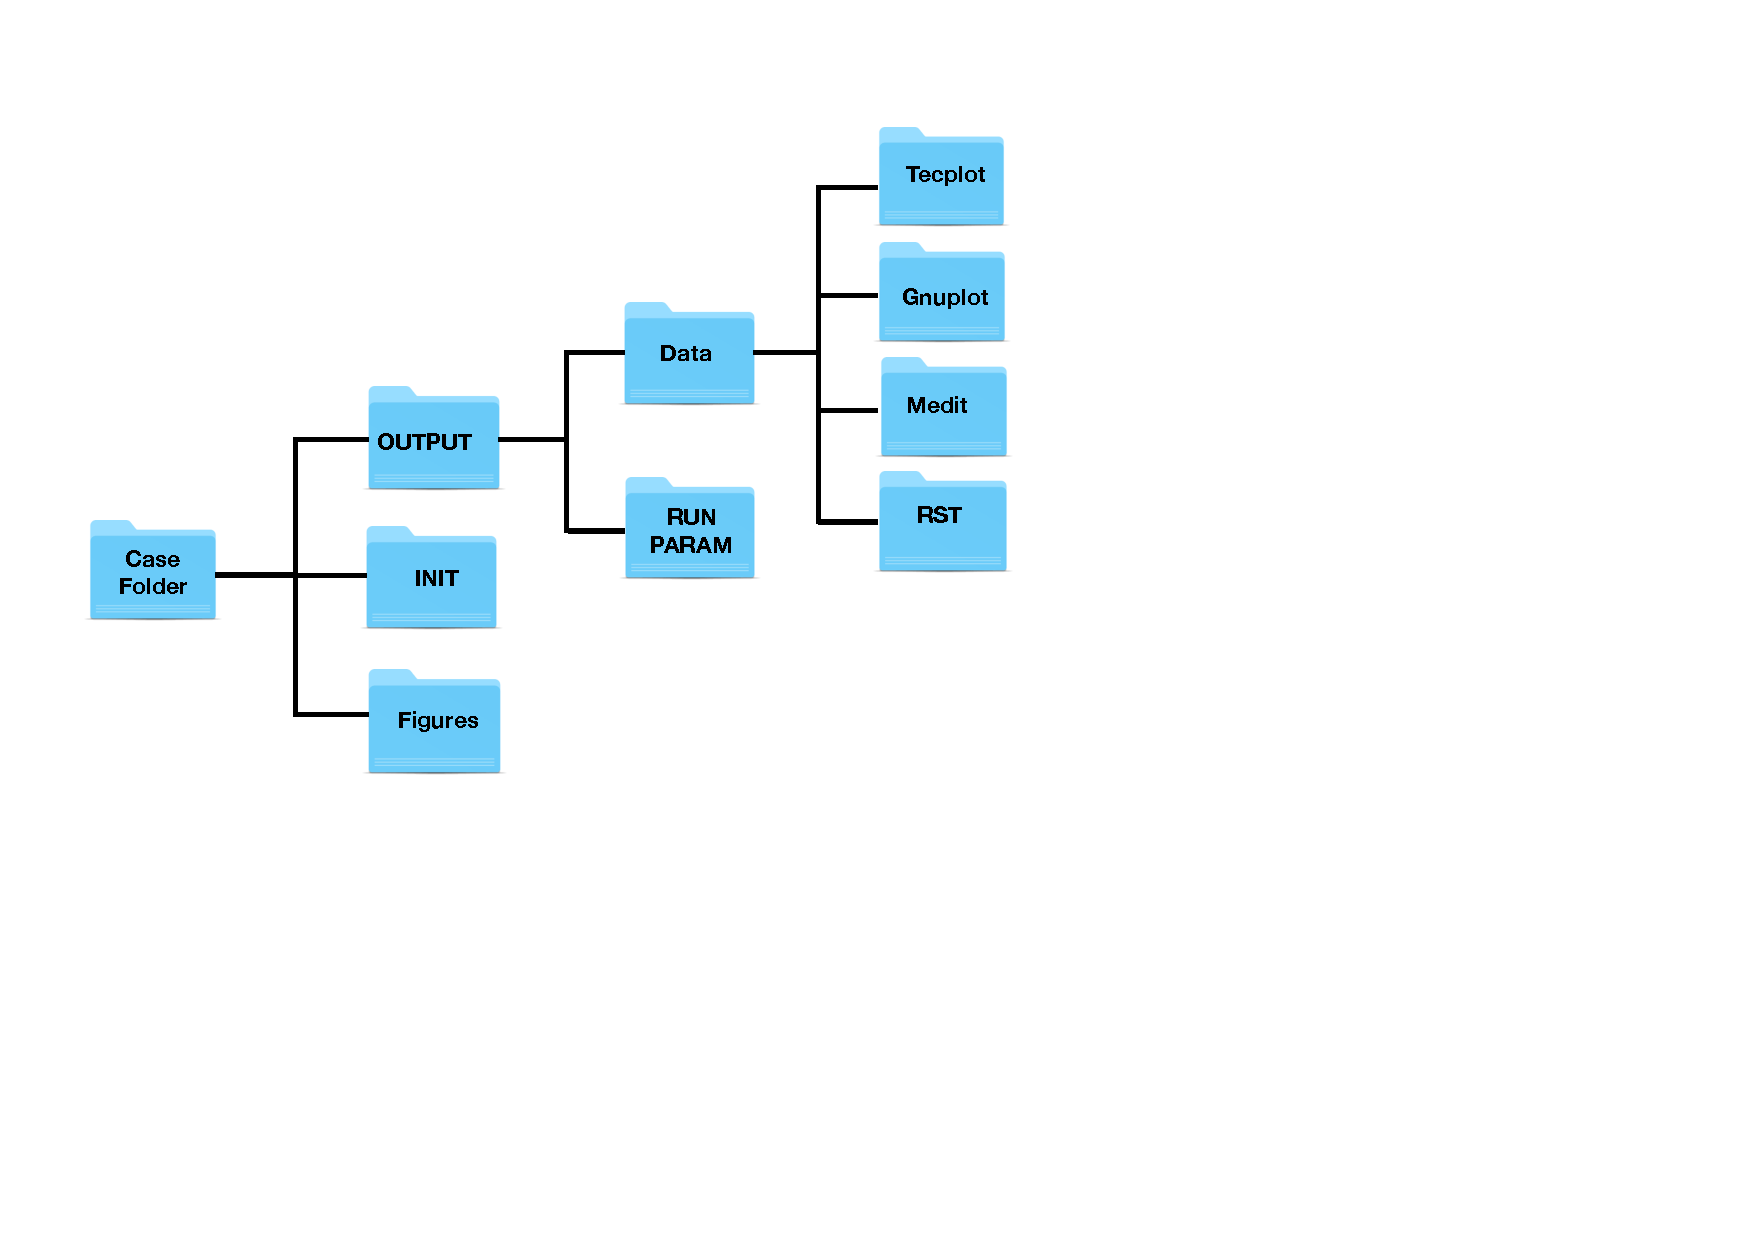
\includegraphics[width=0.8\textwidth]{\figpath/Fig_cap_2/figsCPC_02}
	\end{center}
	\caption{Structure of each Test-case folder. 
	}
	\label{fig-case-folder}
\end{figure}

%\newpage
\subsection{Input parameters}

Physical parameters and parameters related to the run are separated into two files.\\
\textbf{ (1)} The file $param_\_phys.inc$ contains the physical descriptions of the problem:
\begin{itemize}
   \item \textbf{ typeT}: is the finite-element type for the temperature, with possible values \texttt{P2} or \texttt{P1},
   \item \textbf{ Torder}: is the accuracy order of the time integration scheme, with possible values $1$ (Euler scheme) or $2$ (Gear scheme),
   \item \textbf{ scalAdim}: defines the characteristic scales of the problem, see Eq. \ref{eq-adim}. Possible values 1, 2 or 3 correspond to the following choice of the characteristic scales \citep{dan-2014-JCP}:
   \begin{eqnarray} \label{eq-scal1}
    (1) &:&  V_\vref^{(1)} = \frac{\nu_l}{H} \Longrightarrow \ds t_\vref^{(1)} = \frac{H^2}{\nu_l}  \Longrightarrow \Rey=1,\\
      \label{eq-scal2}
     (2) &:& V_\vref^{(2)} = \frac{\alpha}{H} \Longrightarrow \ds t_\vref^{(2)} = t_\vref^{(1)} \Prd  \Longrightarrow \Rey =1/\Prd,\\
      \label{eq-scal3}
     (3) &:& V_\vref^{(3)} = \frac{\nu_l}{H} \sqrt{\frac{\Ray}{\Prd}} \Longrightarrow \ds t_\vref^{(3)} = t_\vref^{(1)} \sqrt{\frac{\Prd}{\Ray}}       \Longrightarrow \Rey = \sqrt{\frac{\Ray}{\Prd}},
\end{eqnarray}

   \item \textbf{ x$_l$, x$_r$, y$_l$, y$_r$}: are the values defining the dimensions of the cavity $[x_l,x_r]\times[y_l,y_r]$,
   \item \textbf{ Pr, Ra, Ste}: are the  Prandtl, Rayleigh and Stefan numbers, see Eq. \ref{eq-Rayleigh} and \ref{eq-RePr},
   \item \textbf{ T$_{hot}$, T$_{cold}$}: are  dimensionless temperatures according to Eq. \ref{eq-adim},
   \item \textbf{ bcu$_1$, bcu$_2$, bcT}: are macros defining the velocity (u) and the temperature (T) boundary conditions.
   \item \textbf{ epsi}: is the half width $\varepsilon$ of the mushy region. \underline{Default value} = $0.01$,
   \item \textbf{ dt}: is the dimensionless time step,
   \item \textbf{ t$_{max}$}: is the dimensionless final time,
   \item \textbf{ Parameters for regularization functions}: \\
 The parameters of the hyperbolic-tangent function in Eq. \ref{eq-smooth}, used to regularize discontinuous functions are set by default as follows:
 \end{itemize}
    \begin{table}[!ht]
    \centering
    \begin{tabular}{*{8}{c}}
     & { f$_{s}$} & {f$_{l}$} & {a$_s$} & {$\theta_s$} & R$_s$ & {$\CKC$} & {b} \\
       \toprule
       {\textit Enthalpy} & 0 & 1/Ste & 1 & 0.01 & 0.01  & - & - \\
       \midrule
       {\textit Carman - Kozeny} & 0 & 1 & 1 & 0.01 & 0.01  & 10$^6$ & 10$^{-7}$ \\
          \midrule
       {\textit Conductivity (water)} & 1 & 2.26/0.578 & 1 & $\theta_f$ & 0.015 & - & - \\
       \bottomrule
     \end{tabular}
    \label{tab-constant}
    \end{table}
   \begin{itemize} 
    \item \textbf{ rho(T) and Drho(T)}: (water cases only) define  the density and its derivative as functions of the temperature, following the model \citep{Gebhart1977}:\\
 
    \begin{table}[!ht]
    \centering
    \begin{tabular}{*{4}{c}}
    	\multicolumn{4}{c}{
      $\rho(T) = \rho_m (1 - \omega | T - T_m |^q),$}\\	\hline
    $\rho_m$ [kg/m$^3$]  & $\omega$ [$^o$C$^{-q}$] & q & $T_m$  [$^o$C] \\
       \toprule
            $999.972$ & $9.2793 \cdot 10^{-6}$ & $1.894816$ & $4.0293$ \\
       \bottomrule
     \end{tabular}
    \label{tab-rho}
    \end{table}
    \item \textbf{ f$_B$(T), df$_B$(T)}: define the buoyancy force and its derivative.
    \end{itemize}

\noindent \textbf{ (2)} The file {\em param$\_$num.inc} contains the parameters controlling the run.\\
\textbf{ Restart parameters:}
\begin{itemize}
   \item \textbf{ Nsave}: the solution is saved every $N\!save$ time steps in the \texttt{Data} folder (see Fig. \ref{fig-case-folder}). The temperature and the velocity fields are saved in \texttt{Tecplot} and \texttt{Medit} folders, while the liquid fraction, the Nusselt number, and the accumulated heat input are saved in the \texttt{Gnuplot} folder.
   \item \textbf{ Nrestart}: restart files (mesh and solution) are saved every $N\!restart$ time steps. Solutions at current and previous iterations, the CPU time, the accumulated heat input $Q_0$, and the time step $dt$ are saved in the folder \texttt{RST}.
   \item \textbf{ Ncondt}: allows the user to stop the run and save the solution properly. \\
   The file \texttt{OUTPUT/zz.condt} is read every $N\!condt$ time steps: if the user replaces the value "0" in this file by "1" the run is stopped. This is a simple solution for a clean stop of the job by the user. \underline{Default value} = $20$.
   \item \textbf{ Nremesh}: the mesh is adapted every $N\!remesh$ iterations. If this parameter is set to "1" the mesh is adapted every time step.
   \item \textbf{ IFrestart}: is a boolean controlling the set up of the initial field. \\
  $I\!Frestart = 0$, the  initial condition is built in the code for each test case. For the PCM melting cases, the PCM is initially motionless at isothermal temperature. 
  	To set-up a smooth initial field, a few time steps (with very small $\delta t$) are computed by increasing progressively the boundary temperature at the hot wall and the Rayleigh number (by continuation).  Outputs are saved in  \texttt{OUTPUT/Data-RST-0}.\\
   $I\!Frestart > 0$, (positive integer values) the solution field previously computed at iteration $I\!Frestart$ is loaded from the folder \texttt{OUTPUT/Data-RST-filenameRST/RST}, \\
   with \texttt{filenameRST} a variable selecting the restart folder. \\
   $I\!Frestart < 0$, (negative integer values), the same principle for loading a solution is used, but from the folder \texttt{INIT}  (see Fig. \ref{fig-case-folder}). The solution fields stored in this folder could come from different previous calculations (\eg a steady state solution or, for the water, the natural convection field before freezing).
\end{itemize}

\noindent \textbf{ Newton parameters:}
\begin{itemize}
   \item \textbf{ epsconv}: is the value of  the stopping criterion for steady cases,
   \item \textbf{ gamma}: is the penalty parameter in  (\ref{eq-time-disc1}). \underline{Default value} = $10^{-7}$,
   \item \textbf{ tolNewton}: is the Newton tolerance $\xi_N$ (see (\ref{eq-Newton-algo})). \underline{Default value} = $10^{-6}$,
   \item \textbf{ newtonMax}: limits the maximum number of iterations in  the Newton algorithm (\ref{eq-Newton-algo}). \\
   \underline{Default value} = $50$,
  % \Blue{\textit {\textbf c$_1$, c$_2$, c$_3$}: \Red{(-- why not negative $a_2$ ?? si c'est trop compliqu� de changer, il faut le laisser tel quel --$>$ } \Blue{C'est modifi� en a$_2$ n�gatif maintenant dans le code)--}  are the coefficients of the time integration scheme: c$_1 =1/$dt, c$_2 = -1/$dt, c$_3 = 0$ correspond to the first order backward Euler scheme and c$_1 =1.5/$dt, c$_2 = -2/$dt, and c$_3 = 0.5/$dt to the second order Gear scheme.}
\end{itemize}

\noindent \textbf{ Mesh parameters:}
\begin{itemize}
   \item \textbf{ nbseg}: is  the number of segments for the discretisation along the $x$ and $y$ directions,
   \item \textbf{ errh}: is the interpolation error level. \underline{Default value} = $0.02$,
   \item \textbf{ hmin, hmax}: are the minimum and maximum edge size, respectively,
   \item \textbf{ adaptratio}: is the ratio for a prescribed smoothing of the metric. For a value less than $1.1$ no smoothing is done. \underline{Default value} = $1.5$,
   \item \textbf{ nbvx}: is the maximum number of vertices allowed in the mesh generator. \underline{Default value} = $50000$.
\end{itemize}

\noindent \textbf{ Output parameters:}
   \begin{itemize}
      \item \textbf{ dircase}: is the name of the output folder,
      \item \textbf{ fcase}: is the prefix-name for ouput files.
      \item \textbf{ Tecplot, Medit, Gnu}: correspond to the name of the visualisation software to be used; the format of the outputs written in \texttt{OUTPUT/Data} (see Fig. \ref{fig-case-folder}) is accordingly set.  The files from the Tecplot folder can be easily read  also with Paraview.
   \end{itemize}
   
\subsection{Outputs}
When a computation starts, the \texttt{OUTPUT} directory is created (see Fig. \ref{fig-case-folder}).
It contains two folders storing the output data and the echo of the run parameters.
The folder \texttt{Data} contains four subdirectories with different output format files of the computed solution. File names are created using  the prefix defined by the parameter \textbf{ fcase}, the current iteration and the current dimensionless time $t$. 
Solution files can be visualized using either Tecplot or any other CFD Visualization tools (Paraview, Visit, etc.). 
Moreover, {\em .gmsh}  (mesh) and {\em .rst} (fields) files are generated in the folder \texttt{RST} to enable restarts of the computation. Note that the folder \texttt{FFglut} contains  \ff scripts that re-read and visualize the RST-files to facilitate the selection of a restart field.  
An {\em .echo} file with a summary of the main parameters, informations on the run and the names of the output files is saved in the folder \texttt{RUNPARAM}.  This directory additionally contains a copy of the {\em .inc} parameter files, allowing an easy identification of each case and preparing an eventual rerun of the same case.


\section{Numerical tests of the accuracy of the numerical method}\label{sec-numconv}

We start by presenting tests of the accuracy of our numerical method. We used the technique of manufactured solutions (\eg \cite{BEC-book-1998-Roache}) which has the advantage of providing an exact solution to a modified problem, related to the initial one.  The general idea is to modify the
original system of equations by introducing an extra source term, such that the new system admits an exact solution
given by a convenient analytic expression. Even though in most cases exact solutions constructed in this way are not physically realistic,
this approach allows one to rigorously verify computations.\\
We tested the space and time accuracy using manufactured solutions for the system of equations (\ref{eq-qmvt})-(\ref{eq-energ}) for a stationary case (Burggraf flow) and a time-dependent one \citep{nourgaliev2016fully}. For both cases, we computed the global error $ \varepsilon$ for different norms in space:
\begin{equation}
  \varepsilon  = \| \Phi_e - \phi_h \|,
  \label{eq-epsconv}
\end{equation}
with $\Phi_e$ the exact solution and $\phi_h$ the numerical solution. Computations were performed for the convection of air ($C=K=1$, $A(\theta)=S(\theta)=0$), with a Rayleigh number $Ra = 10^4$ and a Prandtl number $Pr = 0.71$.


%%%%%%%%%%%%%%%%%%%%%%%%%%%%%%%%%%%%%%%%%%%%
\subsection{Space accuracy: Burggraf stationary flow with thermal effects} \label{subsub-conv-burg}

The Burggraf manufactured solution  is a time-independent recirculating flow inside a square cavity $[ 0 , 1] \times [ 0 , 1]$. It is similar to the well-known  entrained cavity flow, with the difference that the velocity singularity at the top corners of the cavity is avoided. We added to the classical Burggraf flow \citep{Shih-1989,Lamballais-2009} a manufactured solution for the temperature, with 
constant temperature imposed at the top and the bottom walls. Vertical walls are assumed to be adiabatic.
The exact solution of the new flow with thermal effects is:
\begin{eqnarray}
\label{burggraf-u}
   u_1(x,y) &=& \sigma g'(x) h'(y), \\\nonumber
   u_2(x,y) &=& - \sigma g''(x) h(y), \\\nonumber
   p(x,y)   &=& \frac{\sigma}{Re} \left( h^{(3)}(y) g(x) + g''(x)h'(y) \right) + \frac{\sigma^2}{2} g'(x)^2 \left( h(y)h''(y)-h'(y)^2 \right),\\ \nonumber
   T(x,y) &=& T_{c} + (T_{h} - T_{c}) y + a(x) b(y), 
\end{eqnarray}
with $\sigma >0$ a scaling parameter and functions
\begin{eqnarray}
   g(x) &=& \frac{x^5}{5} - \frac{x^4}{2} + \frac{x^3}{3}, \\ \nonumber
   h(y) &=& y^4 - y^2, \\ \nonumber
   a(x) &=& \cos (\pi x), \\ \nonumber
   b(x) &=& y(1-y).
\end{eqnarray}
Note that  the velocity at the top border of the cavity is:
\begin{equation}
u_1(0,1) = 2\sigma (x^4 - 2x^3 + x^2), \quad u_2(x,1) =0,
\end{equation}
which ensures the continuity of the velocity at the corners ($\vec{u}(0,1) =\vec{u}(1,1) =0$), since non-slip walls are imposed for the other borders:
$\vec{u}(x,0) = \vec{u}(0,y) = \vec{u}(1,y) = 0$. 




The forcing terms that have to be added to the momentum and energy (temperature) equation are derived by injecting the exact solution (\ref{burggraf-u}) into the system (\ref{eq-qmvt})-(\ref{eq-energ}):
\begin{eqnarray}
   f_{u_1} &=& 0, \\ \nonumber
   f_{u_2} &=& \sigma^2 h(y) h'(y) \left( g''(x)^2 - g'(x)g^{(3)}(x) \right) \\ \nonumber
   &+& \frac{\sigma}{Re}\left( g^{(4)}(x) h(y) + 2 g''(x)h''(y) + g(x) h^{(4)}(y) \right) \\ \nonumber
   &+& \frac{\sigma^2}{2} g'(x)^2 \left( h(y) h^{(3)}(y) - h'(y)h''(y) \right) - \frac{Ra}{Pr Re^2} T(x,y),\\ \nonumber
   f_T &=& u_1(x,y) a'(x) b(y) + u_2(x,y) \left( T_h - T_c + a(x) b'(y) \right) \\ \nonumber
   &-& \frac{K}{Re Pr} \left( a''(x)b(y) + a(x) b''(y) \right).
\end{eqnarray}
We used the Taylor-Hood finite element (P$_2$ for the velocity and P$_1$ for the pressure)  and tested P$_1$ or P$_2$ finite elements for the temperature.
Figs. \ref{fig-conv-burggraf}a and  \ref{fig-conv-burggraf}b illustrate the streamlines and the temperature field, respectively.
Fig. \ref{fig-conv-burggraf} plots the  discretization error $\varepsilon$  as a function of the grid size $h=\delta x=\delta y$ for the temperature.  Both ${L}^2$ and ${L}^\infty$ norms are displayed. The expected second order accuracy in  ${L}^2$-norm is obtained with  P$_1$ finite elements (Fig. \ref{fig-conv-burggraf}c), while an order exceeding three is 
observed when  P$_2$ finite elements are used (Fig. \ref{fig-conv-burggraf}d).
\begin{figure}[!h]
	\begin{center}
		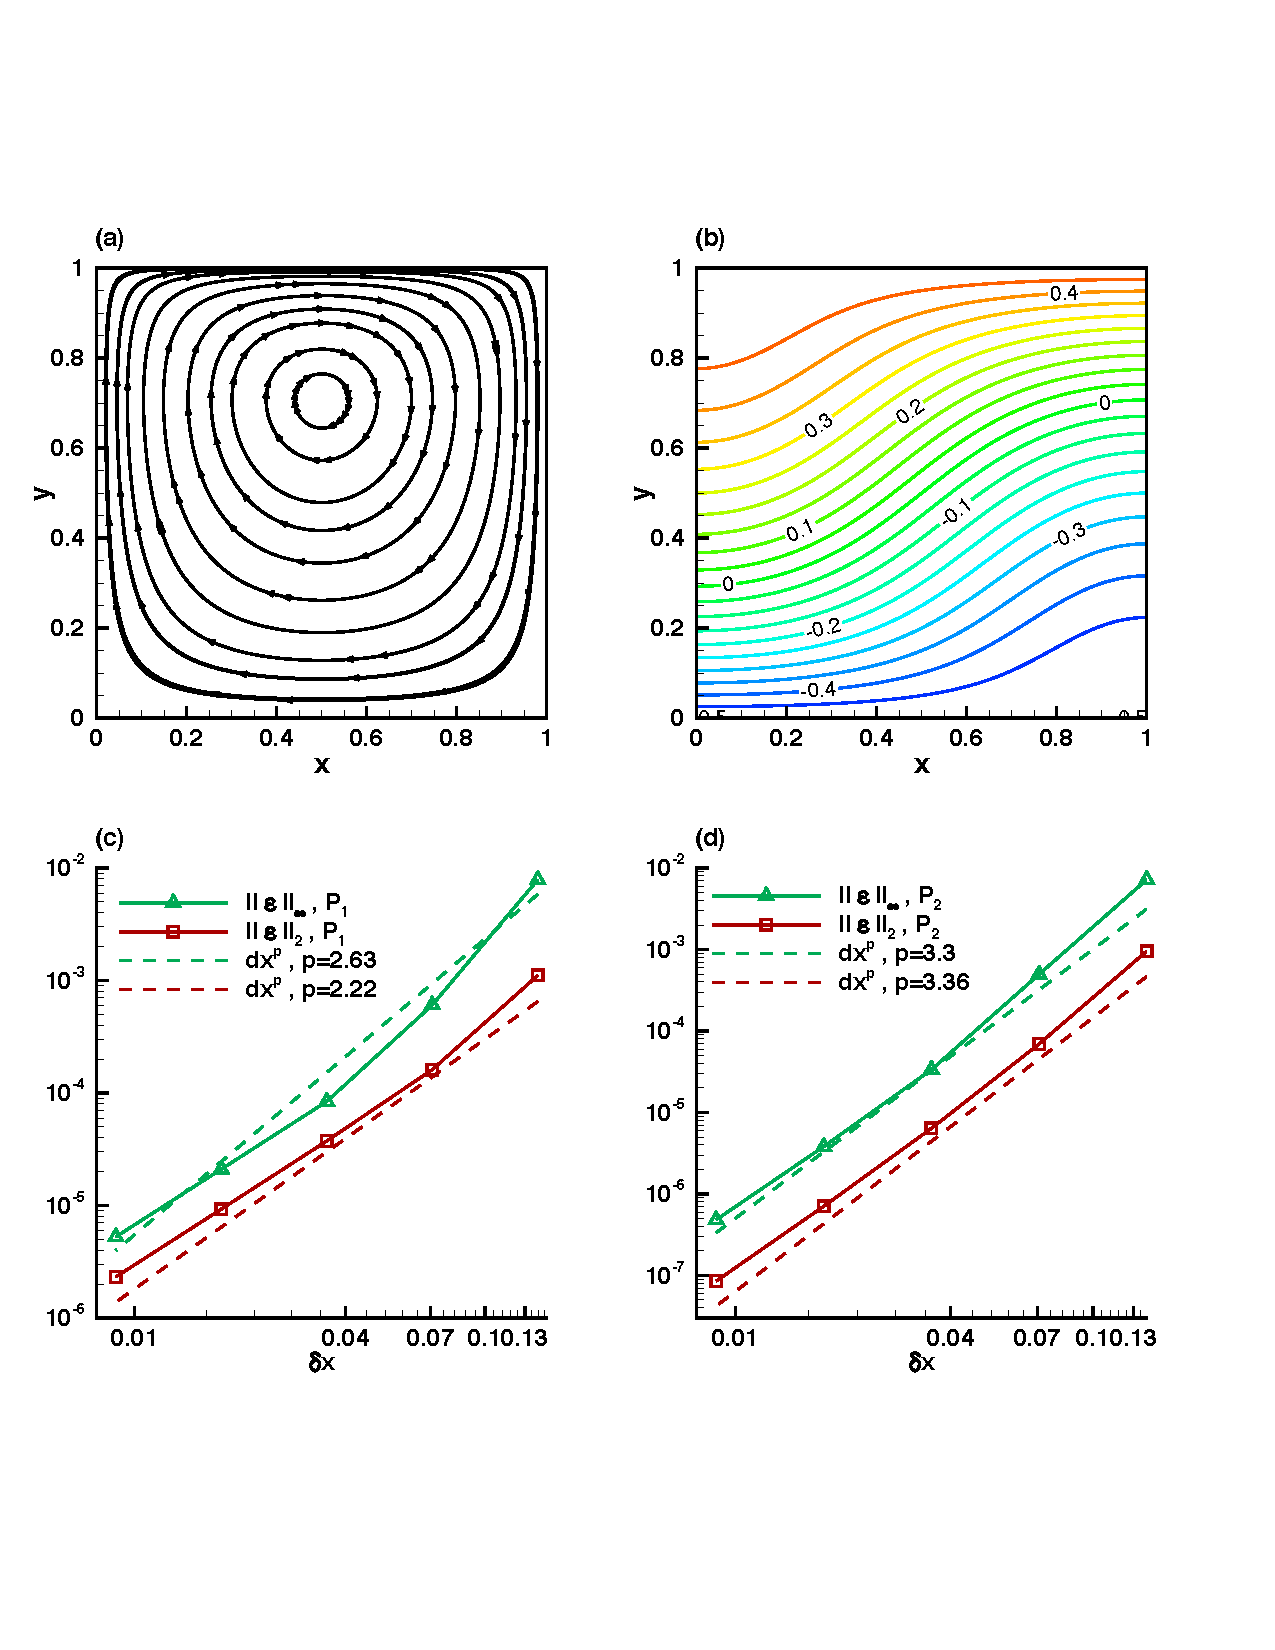
\includegraphics[width=\textwidth]{\figpath/Fig_cap_2/figsCPC_03} 
	\end{center}
	\caption{Burggraf stationary flow with thermal effects used to test the space accuracy of the numerical scheme. Streamlines (a) and temperature contours (b) of the flow field.	
Global error $\varepsilon$ (cf. Eq. \ref{eq-epsconv}) for  the temperature: (c) P$_1$ and (d) P$_2$ finite elements.}
	\label{fig-conv-burggraf}
\end{figure}

%\pagebreak
%%%%%%%%%%%%%%%%%%%%%%%%%%%%%%%%%%%%%%%%%%%
\subsection{Time accuracy: manufactured unsteady solution} \label{subsub-conv-nourg}

To test the time accuracy of the Gear (BDF2) scheme, we used the manufactured time-dependent solution suggested in \cite{nourgaliev2016fully}:
\begin{align}
\label{eq-manufN}
	u_1(x,y,t) &=& \left( \delta U_0 + \alpha_u \, \sin(t) \right) \, \cos(x+ \gamma_1 t) \, \sin(y+ \gamma_2 t), \\ \nonumber
	u_2(x,y,t) &=& - \left( \delta U_0 + \alpha_u \sin(t) \right) \, \sin(x+ \gamma_1 t) \, \cos(y+ \gamma_2 t), \\ \nonumber
	T(x,y,t) &=& \bar{T} + \left( \delta T_0 + \alpha_t \sin(t) \right) \, \cos(x+ \gamma_1 t) \, \sin(y+ \gamma_2 t), \\ \nonumber
	p(x,y,t) &=& \bar{P} + \left(\delta P_0 + \alpha_p \sin(t) \right) \, \sin(x+ \gamma_1 t) \, \cos(y+ \gamma_2 t), 
\end{align}
The values of the constants are reported in Table \ref{tab-constant}.
\begin{table}[!h]
\centering
\begin{tabular}{*{10}{c}}
 % \toprule
  $\gamma_1$ & $\gamma_2$ & $\bar{P}$ & $\bar{T}$ & $\delta P_0$ & $\delta T_0$ & $\delta U_0$ & $\alpha_p$ & $\alpha_u$ & $\alpha_t$\\
   \midrule
  $0.1$ & $0.1$ & $0$ & $1.0$ &  $0.1$ & $1.0$ & $1.0$ & $0.05$ & $0.4$ & $0.1$ \\
 % \bottomrule
 \end{tabular}
\caption{Parameter for the time-dependent manufactured solution (\ref{eq-manufN}).}
\label{tab-constant}
\end{table}
The corresponding forcing source terms are:
\begin{eqnarray}
	f_{u_1} &=& \alpha_u \, \cos(t) \, \cos(a) \sin(b) - U_c \, \gamma_1 \, \sin(a) \sin(b) + U_c \, \gamma_2  \, \cos(a)\cos(b) \\ \nonumber
	  & & - U_c \,  u_1(x,y,t) \, \sin(a) \sin(b) + U_c \,  u_2(x,y,t) \, \cos(a) \cos(b)
	  + P_c \, \cos(a) \cos(b)\\ \nonumber
	  & & + \frac{2}{Re} \, u_1(x,y,t), \\	  \nonumber
	f_{u_2} &=& - \alpha_u \,  \cos(t)  \, \sin(a) \cos(b) - U_c \,  \gamma_1  \,  \cos(a) \cos(b) + U_c \,  \gamma_2 \,  \sin(a)\sin(b) \\ \nonumber
		  & & - U_c \,  u_1(x,y,t)  \,  \cos(a) \cos(b) + U_c  \, u_2(x,y,t)  \,  \sin(a) \sin(b)
		  -  P_c  \,  \sin(a)  \,  \sin(b)\\ \nonumber
		  & &+ \frac{2}{Re} \,  u_2(x,y,t)
		  - \frac{Ra}{Pr Re^2} \,  T(x,y,t), \\  \nonumber
	f_{T} &=& \alpha_t \,  \cos(t) \,  \cos(a) \sin(b) -  T_c  \,  \gamma_1 \,  \sin(a) \sin(b) + T_c \,   \gamma_2  \,  \cos(a)\cos(b) \\ \nonumber
		  & &-  T_c \,  u_1(x,y,t)  \,  \sin(a) \sin(b)  
		  +   T_c  \,  u_2(x,y,t)  \, \cos(a) \cos(b) 
		  + \frac{2 K}{Re Pr} \,  T_c  \, \cos(a) \sin(b), \\ \nonumber
\end{eqnarray}
where $a = (x+ \gamma_1 t), \,
b = (y+ \gamma_2 t)$ and  
$U_c = (\delta U_0 + \alpha_u \sin(t)), \,
	T_c = (\delta T_0 + \alpha_u \sin(t)), \,
	P_c = (\delta P_0 + \alpha_u \sin(t))$.

Guided by  the results obtained  in \S \ref{subsub-conv-burg} for the space accuracy, we fixed the grid size to $h=dx = 0.01$ to ensure small spatial discretization errors.
For diminishing values of the time step $\delta t$, the solution was evolved in time up to the time instant $t_{max} = \pi$ at which the error  (\ref{eq-epsconv}) was computed. 
The time convergence is displayed in Fig. \ref{fig-conv-bdf2} for the temperature variable. 
The expected second order convergence in time is obtained for both P$_1$ (Fig. \ref{fig-conv-bdf2}a) and P$_2$ (Fig. \ref{fig-conv-bdf2}b) discretizations of the temperature.

\begin{figure}[!h]
	\begin{center}
		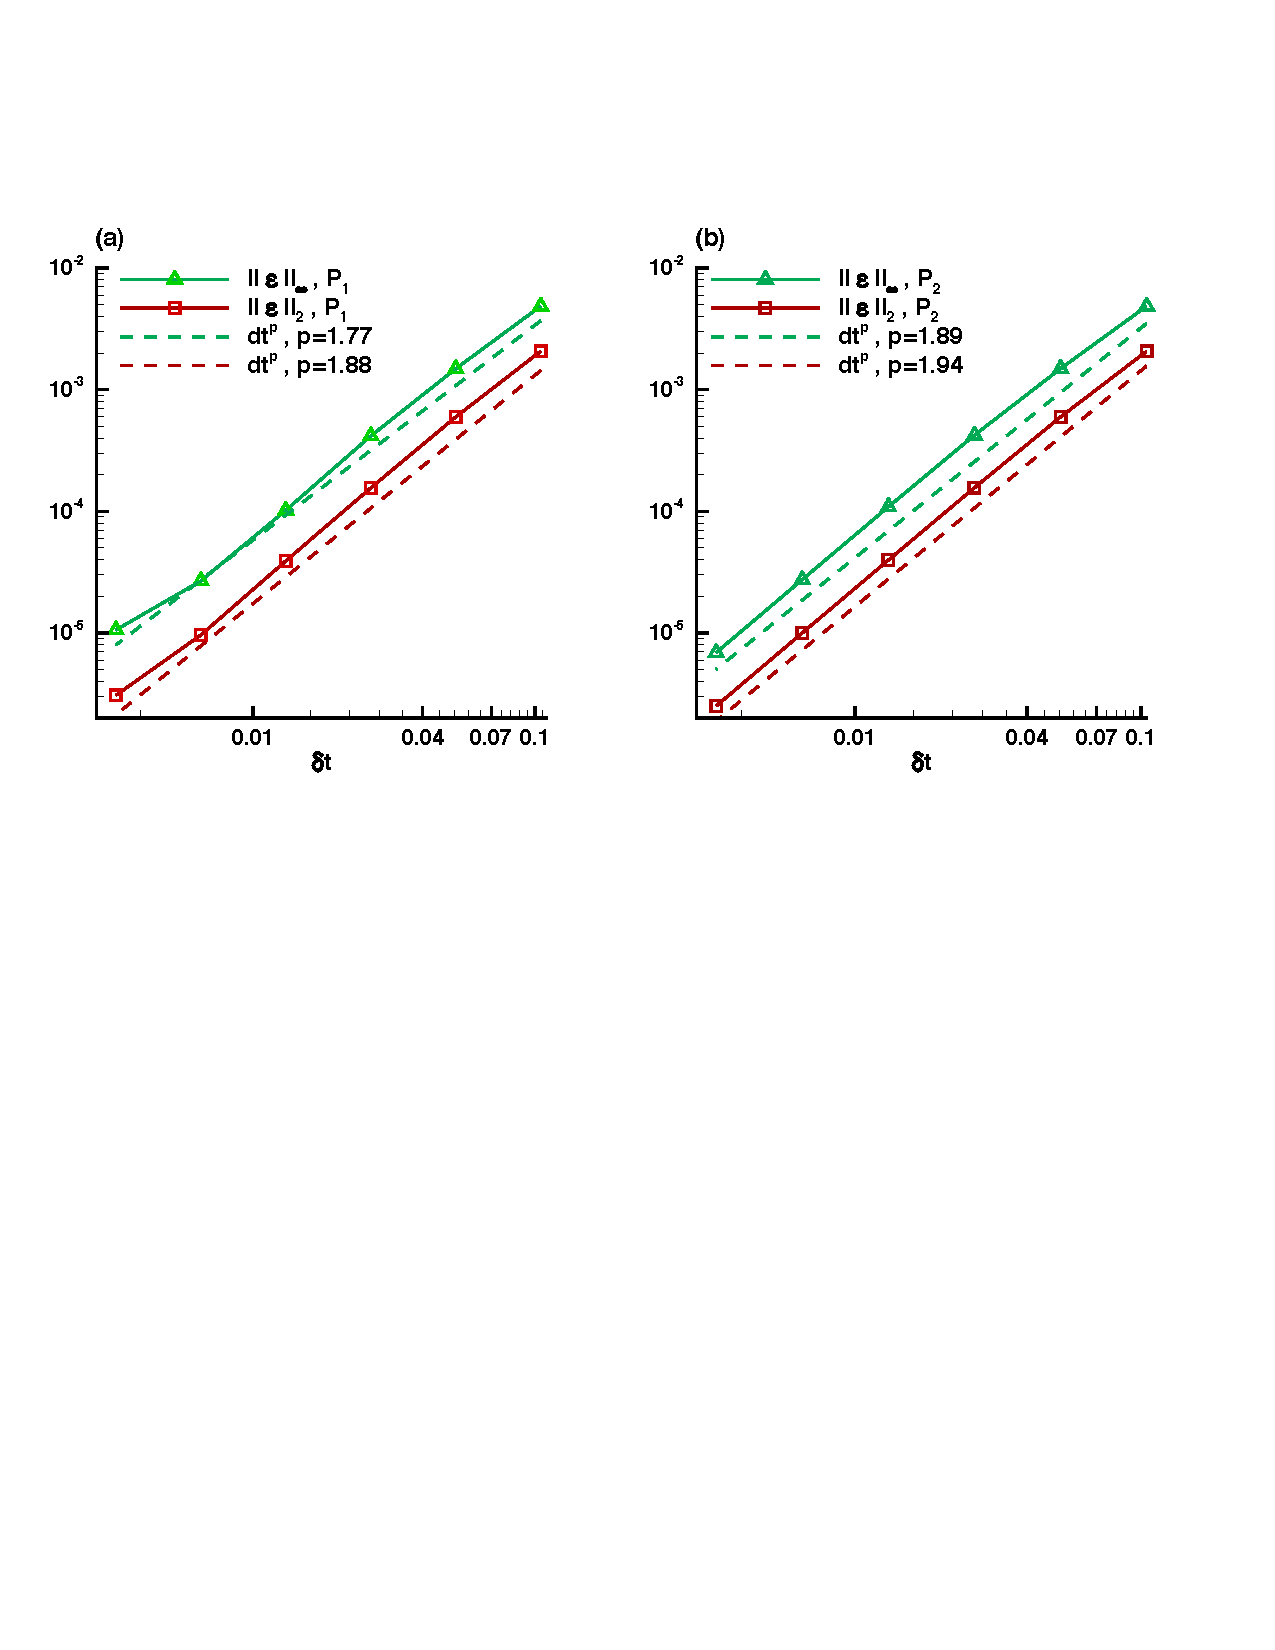
\includegraphics[width=\textwidth]{\figpath/Fig_cap_2/figsCPC_04} 
	\end{center}
	\caption{Time accuracy of the numerical scheme tested using the time-dependent manufactured solution of \cite{nourgaliev2016fully}. Evolution of the global error $\varepsilon$ given in (\ref{eq-epsconv}) for  the temperature at $t_{max} = \pi$. Discretizations using: (a) P$_1$ and (b) P$_2$ finite elements.}
	\label{fig-conv-bdf2}
\end{figure}

\section{Domain decomposition method with FreeFem++: FFDDM}
Solving the Navier-Stokes-Boussinesq systems of Eqs. \ref{eq-weak-all} - \ref{eq-weak-energy} in three-dimensional configurations could generate a large problem size.
The natural convection of air in a cube of dimensions $[0,1]^3$ with $40 \times 40 \times 40$ uniform grids involves indeed $3$ millions of unknowns (d.o.f.) in the linear system, when a $P_1$ finite element is considered for the temperature.
For such a large size of problem, memory lack issue can rapidly arise with sequential algorithms.
It is thus essential to distribute data among several processors.

A natural approach is the domain decomposition method (DDM).
DDM aims at dividing the computational domain in many subdomains on which we solve local problems with the adequate interface conditions.
Two families of DDM exists: non-overlapping methods and overlapping methods such as Schwarz method.

\noindent We perform in this work a domain decomposition Schwarz method, enhanced by coarse space corrections through the \ff library \texttt{ffddm}.
This enrichment with coarse space is mandatory in the present study to avoid the lack of robustness related to the One-Level method. 
It is well-known indeed that the main drawback of such One-Level methods is their convergence rate that depends on the number of subdomains,
resulting to a poor scale for large problems. 
This is mostly due to a lack of global communication between subdomains that exchanges informations with its direct neighbors only.
The additional coarse space has consequently the task to spread the informations to all subdomains at each iteration.

%We use the recent library \texttt{ffddm} that makes available in \ff state-of-the-art scalable Schwarz domain decomposition methods (DDM).
%FFDDM (FreeFem++ Domain Decomposition Method) is a parallel part of FreeFem++ allowing to use parallel solver in FreeFem++.
 %The DDM approach is based on a Schwarz method enhanced by coarse space corrections.
%The data distribution among the processor is done via an overlapping domain decomposition and a related linear algebra.
%The linear system is then solved by using the domain decomposition method as preconditioners to the GMRES Krylov method.

The data distribution among the processor is done via an overlapping domain decomposition and a related linear algebra.
To enable parallel computing, the mesh is first split into subdomains using \texttt{Scotch} or \texttt{Metis} libraries. 
Fig. \ref{fig:mesh-partition} illustrates the domain decomposition of a cube of dimensions $[0,1]^3$ into $8$ subdomains with \texttt{Metis} graph partitioner. 
Mesh adaptivity using metrics control makes possible the optimisation of the distribution of mesh elements.
%Then, a  domain decomposition Schwarz method, enhanced by coarse space corrections, is used through the \ff library \texttt{ffddm}. 


\begin{figure}
	\begin{center}
		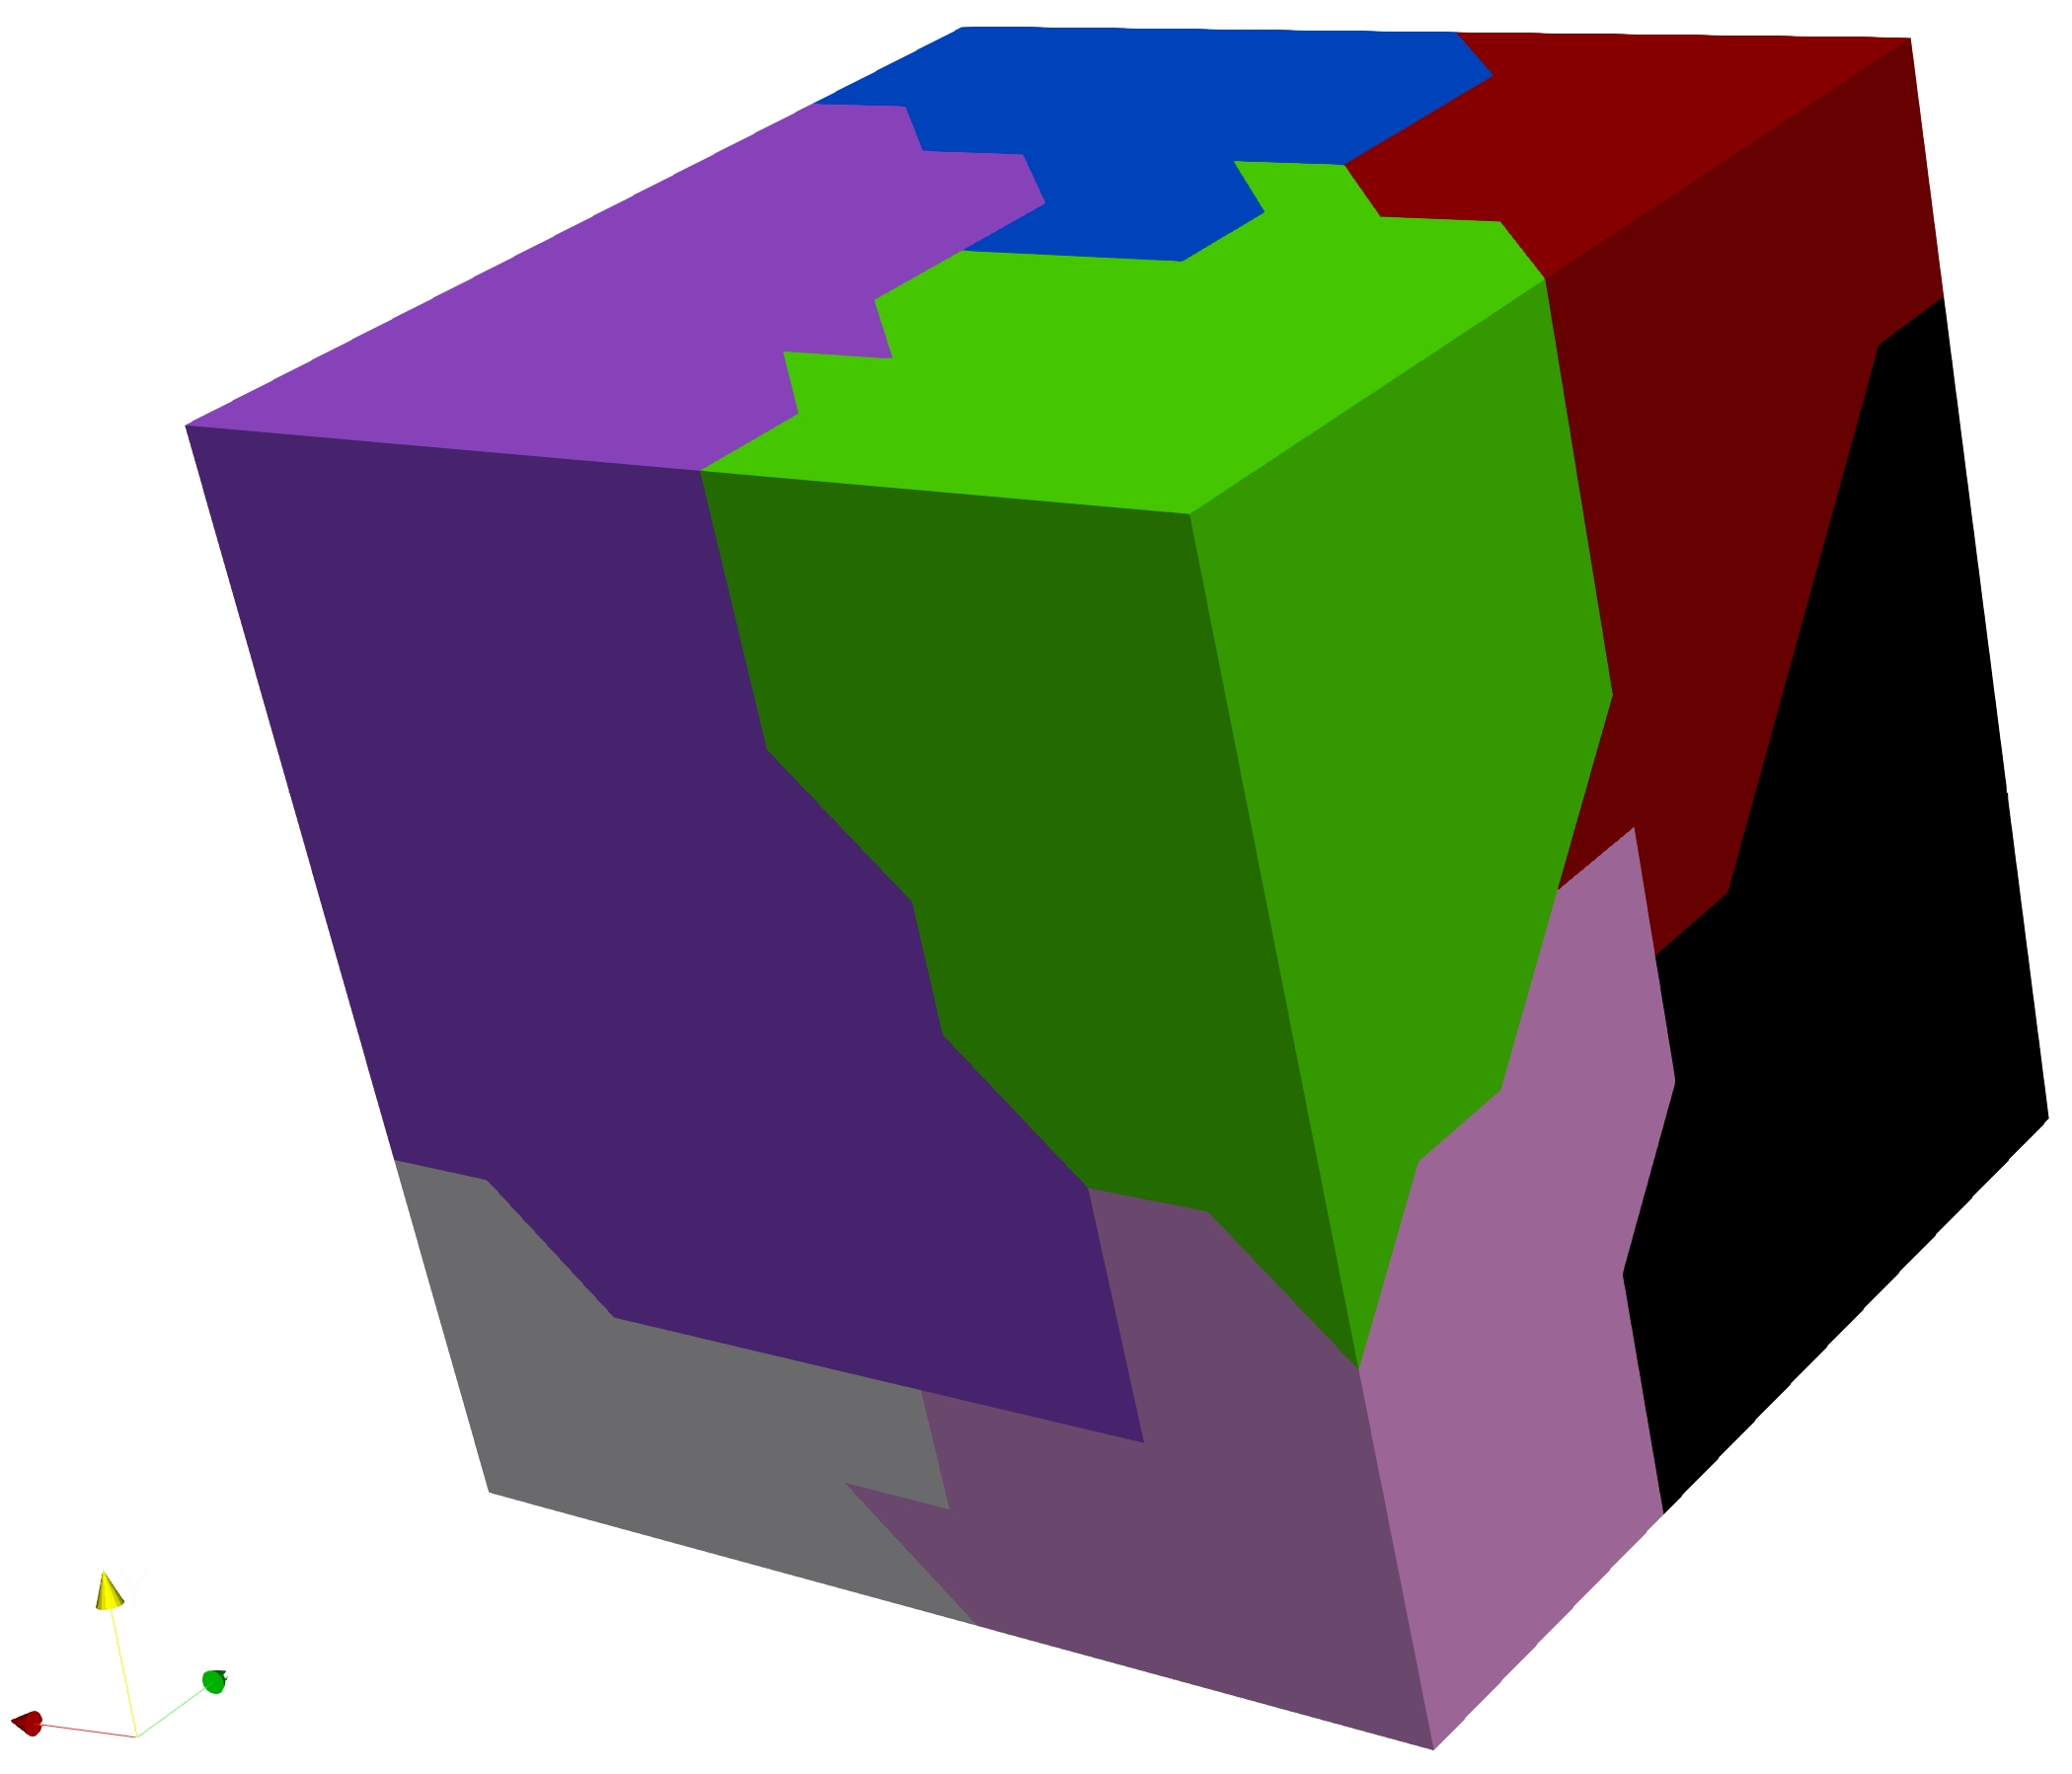
\includegraphics[width=.5\textwidth]{\figpath/Fig_cap_meth-num/Partitionning}
	\end{center}
	\caption{Partition of $\Omega = [0,1]^3 $ into $8$ subdomains with \texttt{Metis} partitioner.}
	\label{fig:mesh-partition}
\end{figure}

\noindent The  final linear system of Eqs. \ref{eq-newton-C1} - \ref{eq-newton-C3} is solved in parallel using a GMRES Krylov method, with an Optimized Restricted Additive Schwarz (ORAS) preconditioner.  
To solve the linear equation $A x = rhs$, the ORAS preconditionner reads
\begin{equation}
   M_{RAS}^{-1} = \sum_{j=1}^{\mathcal{N}} R^T_j D_j (R_j A R^T_j)^{-1} R_j,
\end{equation}
$R_j$ denote the restriction operators and $D_j$ are square diagonal matrices.
Local matrices are defined as:
\begin{equation}
   A_j = R_i A R_i^T.
\end{equation}
The duplicated unknowns due to the overlap between subdomains are coupled via a partition of unity
\begin{equation}
   I = \sum_{i=1}^{\mathcal{N}} R_i^T D_i R_i.
\end{equation}
Thus, the global solutions $U$ is defined as:
\begin{equation}
  U = \sum_{i=1}^{\mathcal{N}} R_i^T D_i R_i U =  \sum_{i=1}^{\mathcal{N}} R_i^T D_i U_i.
\end{equation}

We assess the strong scalability of the ORAS preconditioner on the 3D differentially heated cube cavity.
We vary the number of subdomains while the global system size is fixed.
With a P$_2$ finite element for the temperature, we solve $7.2$ million of unknowns (d.o.f).
The subdomain is decomposed into subdomains with \texttt{Metis}, ranging from $48$ to $400$ subdomains.
Fig. \ref{fig-scalability} illustrates the evolution of the total wall clock time for different subdomains, in which a good speed up is observed.
From $48$ to $320$ we observe a linear speed up. 
The total runtime passes from $2$ hours for $48$ subdomains to $15$ minutes for $320$ subdomains.
The linear speed up is then slightly lost for $400$ subdomains but remains reasonable.
In Tab. \ref{tab-scalability} we detail the timing relative to this test.
The column "Factorization" denotes the time spent in the factorization of the local submatrices and "GMRES" gives the time taken by GMRES to solve the global linear system
by the domain decomposition algorithm.

\begin{figure}%[!htbp]
\begin{minipage}{\linewidth}
\begin{center}
 {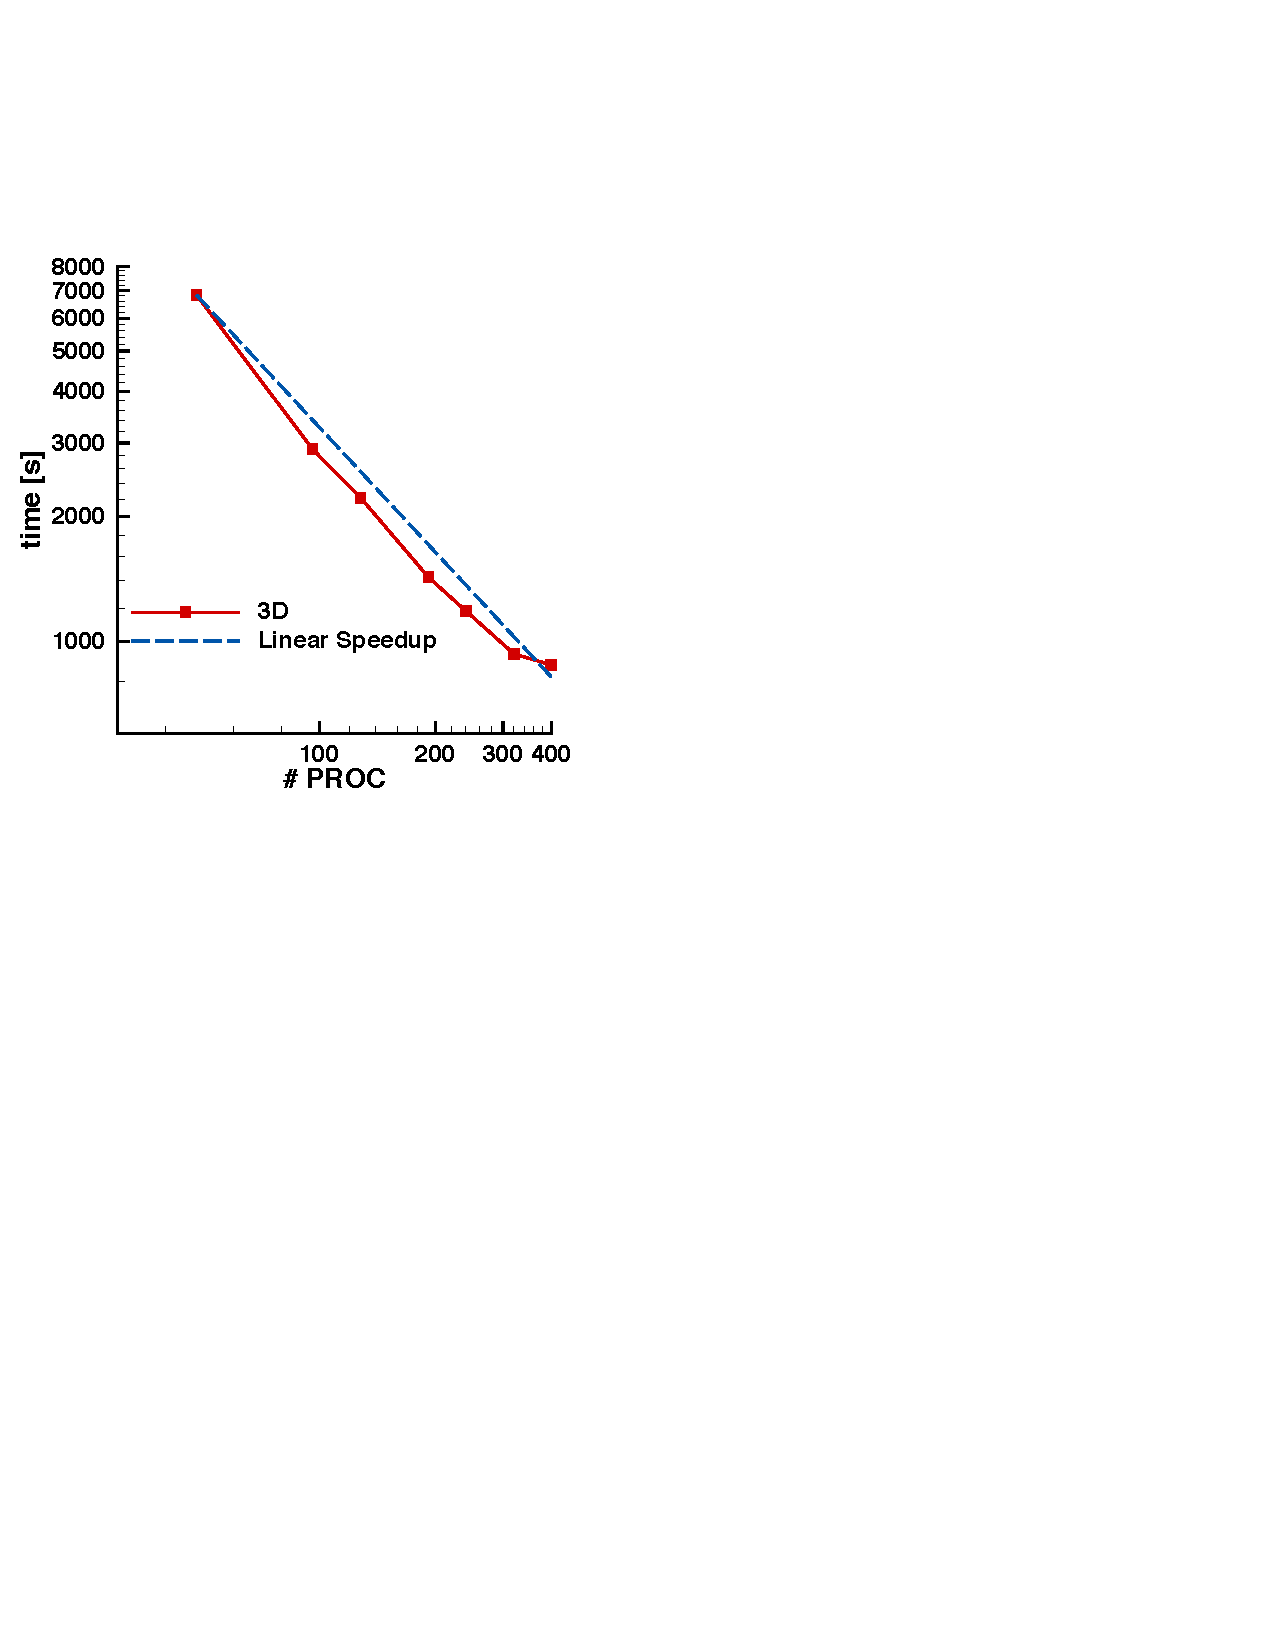
\includegraphics[width=.49\textwidth]{\figpath/Fig_cap_natconv/Scal_ffddm_2level}}
 {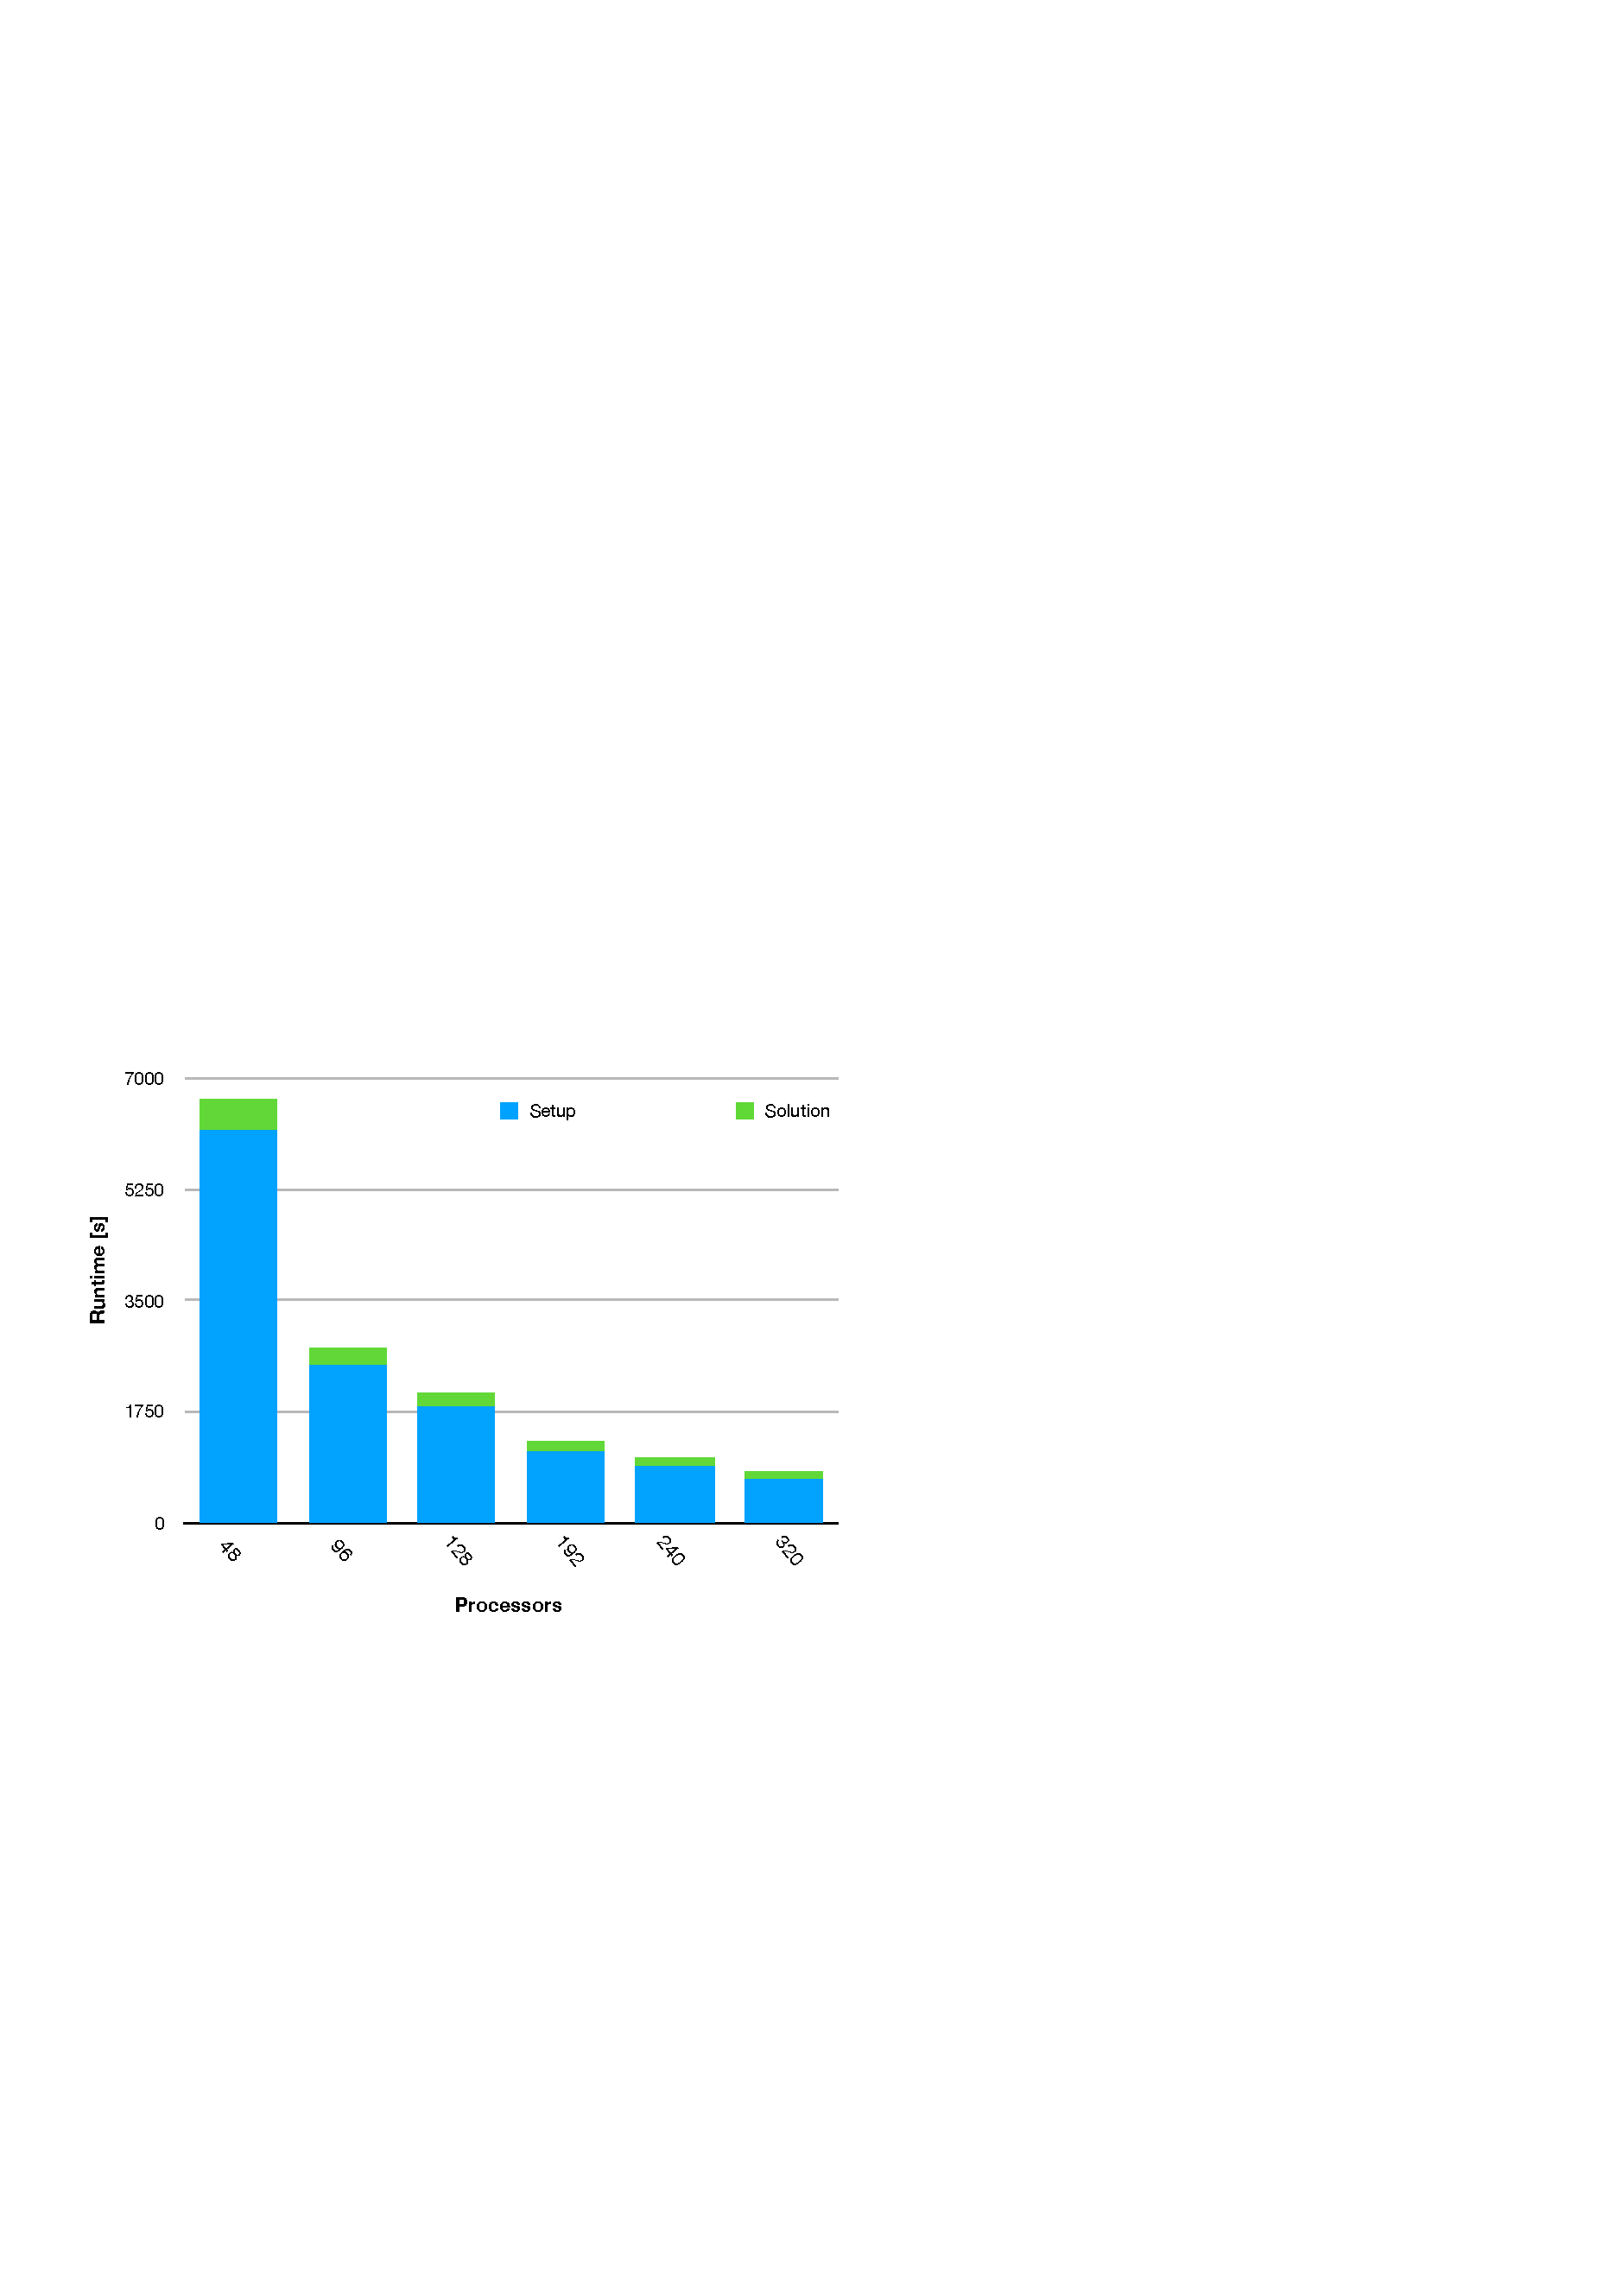
\includegraphics[width=.5\textwidth]{\figpath/Fig_cap_2/scal_ffddm_P2}}
\end{center}
\end{minipage}
\caption{Strong scalability of the ORAS preconditioner: $7.2$ millions of d.o.f and subdomains ranging from $48$ to $400$.}
\label{fig-scalability} 
\end{figure}

\begin{table}
	\begin{center}
		\begin{tabular}{cccc}
			 $\mathcal{N}$ & Factorization (s)  & GMRES (s)  & Total Step (s) \\ \hline \hline
			 48 & 6186.33  & 473.66  &  6659.99 \\
			 96 & 2468.68  & 283.099 &  2751.779 \\
			 128 & 1814.26 &  237.853 &   2052.113\\
			 192 & 1111.5  &   169.174 &  1280.674 \\
			 240 & 889.422  & 146.539 &  1035.961\\
			 320 & 674.204   &  114.346 & 788.55 \\
			 400 & 614.418  &  107.422 &  721.84\\ \hline
		\end{tabular}
	\end{center}
	\caption {Strong scaling experiment in 3D differentially heated cavity. $7.2$ millions of d.o.f and subdomains ranging from $48$ to $400$. }
	\label{tab-scalability}
\end{table}

%%%%%%%%%%%%%%%%%%don't forget if needed %%%%%%%%%%%%%%%%%%%%%
%\section[toc version]{title version%
%              \sectionmark{head version}}
%\sectionmark{head version}
%%%%%%%%%%%%%%%%%%%%%%%%%%%%%%%%%%%%%%%%%%%%%%%%%%%%%%%%%%%%%%
\def\titcourt{A finite-element toolbox}
\def\titlong{A finite-element toolbox for the simulation of phase-change systems with natural convection}
%%%%%%%%%%%%%%%%%%%%%%%%%%%%%%%%%%%%%%%%%%%%%%%%%%%%%%%%%%%%%%%%
\chapter[\titlong]{\titlong%
              \chaptermark{\titcourt}}
\chaptermark{\titcourt}
\label{chap-ToolBox}
%%%%%%%%%%%%%%%%%%%%%%%%%%%%%%%%%%%%%%%%%%%%%%%%%%%%%%%%%%%%%%%%
%%%%%%%%%%%%%%%%%%%%%%%%%%%%%%%%%%%%%%%%%%%%%%%%%%%%%%%%%%%%%%%%


%\section{A finite-element toolbox for the simulation of phase-change systems with natural convection}\label{sec-desc-prog}

The methods described previously were implemented in a 2D toolbox based on \ff software.
In this section we first describe the architecture of the programs and the organisation of files.
Then we focus on the list of input parameters and the structure of output files.
%
\begin{figure}[!h]
	\begin{center}
		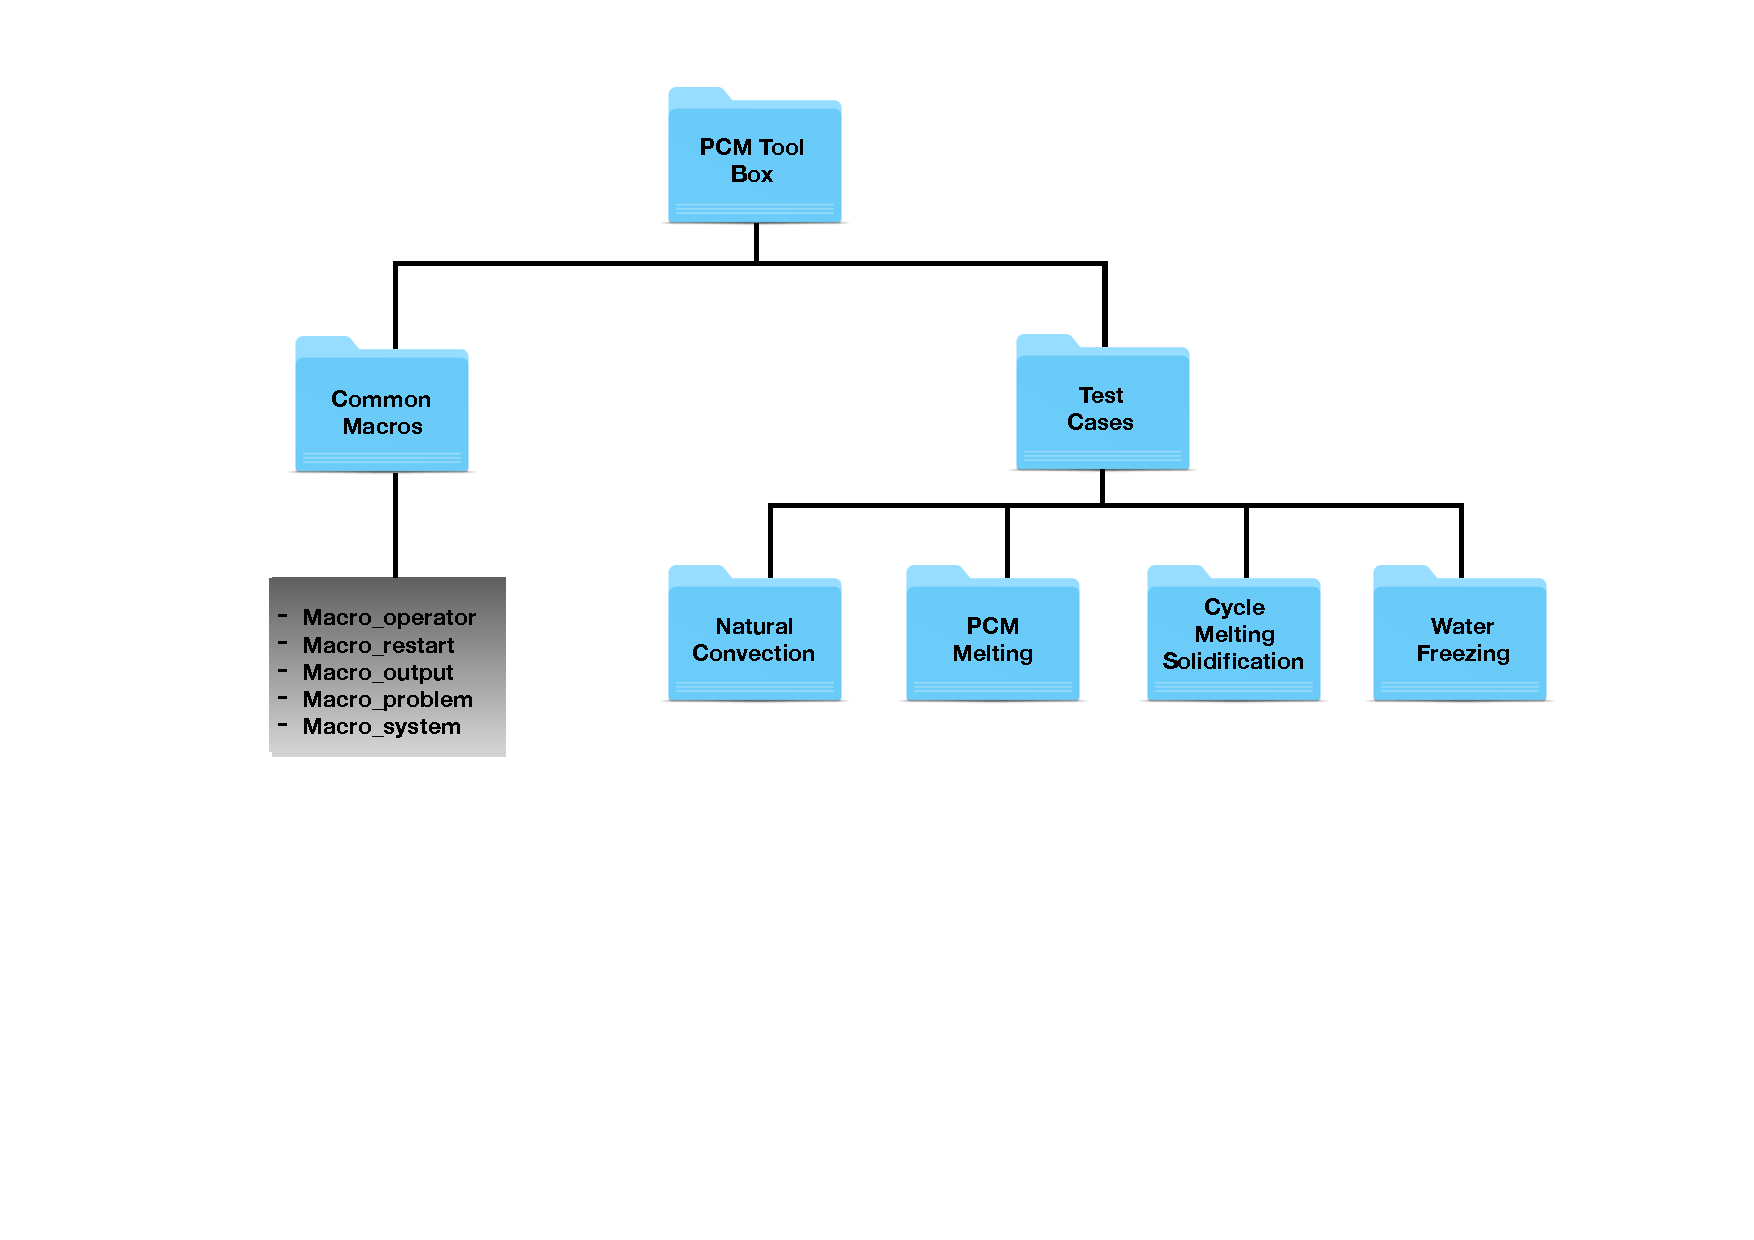
\includegraphics[width=0.9\textwidth]{\figpath/Fig_cap_2/FOLDER_arbor_3}
	\end{center}
	\caption{Folder tree structure of the FreeFem++ toolbox to solve phase change problems. Test cases and common macros are separated into two folders.}
	\label{fig-folder-tree}
\end{figure}

\section{Program architecture}
Figure \ref{fig-folder-tree} gives a schematic overview of the content of the toolbox. All files are provided in a directory called \texttt{PCM-Toolbox}.  Many detailed comments are included in the programs, with direct link to the mathematical expressions used in the paper. The used \ff syntax was intentionally kept at a low level of technicality and supplemented with detailed comments when specific more technical syntax was used.

This directory is organized as follows:
\begin{enumerate}
   \item The directory \texttt{Common-Macros} contains five files:\\
$\bullet$ {\em Macro$\_$operator.idp} includes macros and functions defining mathematical operators,\\
$\bullet$ {\em Macro$\_$problem.idp}: macros defining the variational formulation of the problem,\\
$\bullet$ {\em Macro$\_$restart.idp}: macros used to start a new simulation from a saved field,\\
$\bullet$ {\em Macro$\_$output.idp}: macros used to save the solution with different formats,\\
$\bullet$ {\em Macro$\_$system.idp}: macros identifying the OS and defining specific OS-commands.

   \item The directory \texttt{Test-Cases}  contains four subdirectories, each of them defining one of the following applications:\\
    $\bullet$  natural convection of air or water in a differentially heated square cavity, \\
    $\bullet$  melting of a PCM stored in containers of different shapes,\\
    $\bullet$  melting followed by solidification of a rectangular PCM,\\
    $\bullet$  freezing of pure water in a square cavity.\\
   Each subdirectory contains  three files: {\em NEWTON$\_$\$case.edp} is the main \ff script file, $param_\_phys.inc$ defines the physical parameters and $param_\_num.inc$ the numerical parameters. For example, to run the natural convection case of air in a square cavity, the user can use the following command in a terminal window:
  \texttt{FreeFem++ NEWTON$\_$stat$\_$natconv.edp}.\\
  The folder structure of each test case is illustrated in Figure \ref{fig-case-folder}.
  The obtained solutions are saved in the folder \texttt{OUTPUT/Data}. Depending on the output format selected by the user,  data files are generated in specific folders for being visualized with: Tecplot, Paraview, Gnuplot or Medit. We also provide in the folder \texttt{Figures} ready-made layouts for these visualisation softwares. The user can thus obtain the figures from this paper using  newly generated data. More details about the output structure are given below.
\end{enumerate}

\begin{figure}[!h]
	\begin{center}
		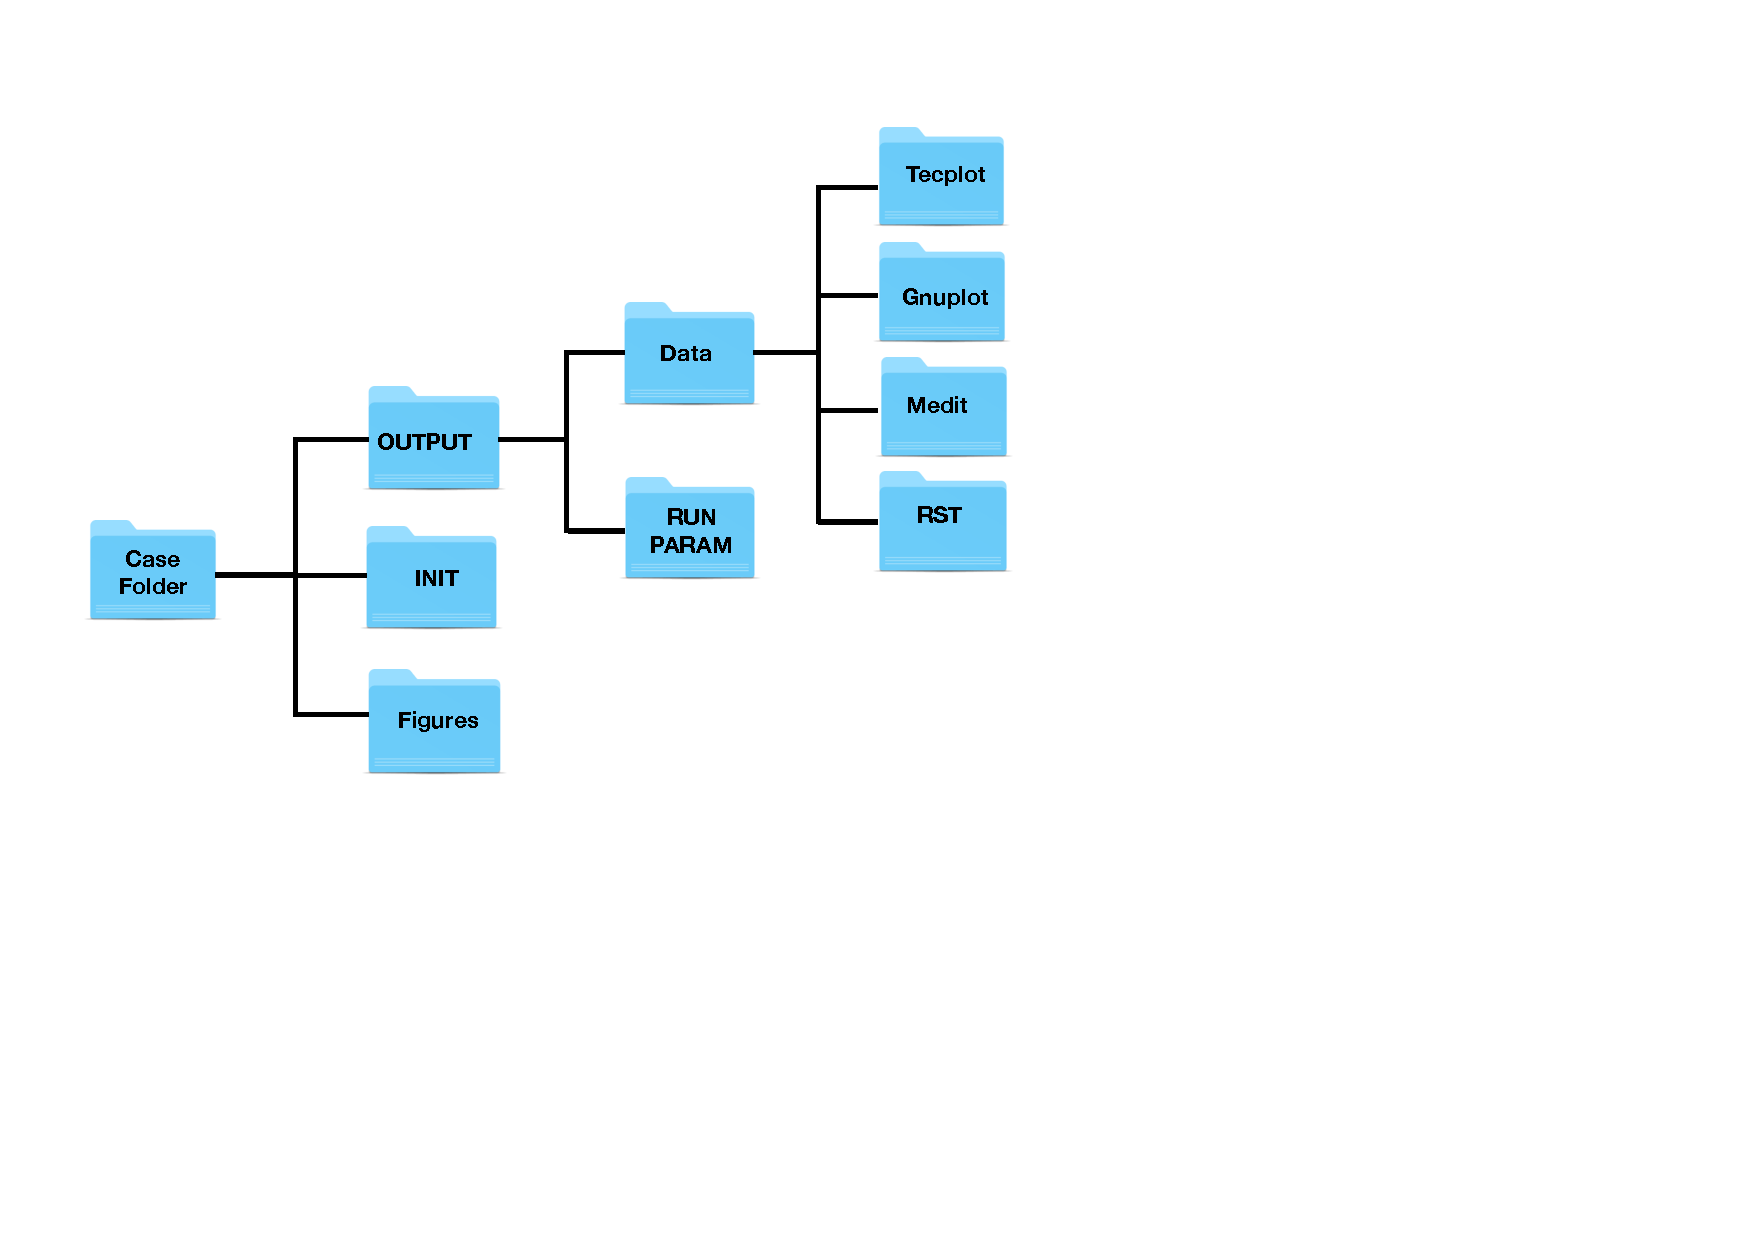
\includegraphics[width=0.7\textwidth]{\figpath/Fig_cap_2/figsCPC_02}
	\end{center}
	\caption{Structure of each Test-case folder. 
	}
	\label{fig-case-folder}
\end{figure}

\section{Input parameters}

Physical parameters and parameters related to the run are separated into two files.\\
{\bf (1)} The file $param_\_phys.inc$ contains the physical descriptions of the problem:
\begin{itemize}
   \item {\bf typeT}: is the finite-element type for the temperature, with possible values \texttt{P2} or \texttt{P1},
   \item {\bf Torder}: is the accuracy order of the time integration scheme, with possible values $1$ (Euler scheme) or $2$ (Gear scheme),
   \item {\bf scalAdim}: defines the characteristic scales of the problem, see (\ref{eq-adim}). Possible values 1, 2 or 3 correspond to the following choice of the characteristic scales \citep{dan-2014-JCP}:
   \begin{eqnarray} \label{eq-scal1}
    (1) &:&  V_\vref^{(1)} = \frac{\nu_l}{H} \Longrightarrow \ds t_\vref^{(1)} = \frac{H^2}{\nu_l}  \Longrightarrow \Rey=1,\\
      \label{eq-scal2}
     (2) &:& V_\vref^{(2)} = \frac{\alpha}{H} \Longrightarrow \ds t_\vref^{(2)} = t_\vref^{(1)} \Prd  \Longrightarrow \Rey =1/\Prd,\\
      \label{eq-scal3}
     (3) &:& V_\vref^{(3)} = \frac{\nu_l}{H} \sqrt{\frac{\Ray}{\Prd}} \Longrightarrow \ds t_\vref^{(3)} = t_\vref^{(1)} \sqrt{\frac{\Prd}{\Ray}}       \Longrightarrow \Rey = \sqrt{\frac{\Ray}{\Prd}},
\end{eqnarray}
   \item {\bf x$_l$, x$_r$, y$_l$, y$_r$}: are the values defining the dimensions of the cavity $[x_l,x_r]\times[y_l,y_r]$,
   \item {\bf Pr, Ra, Ste}: are the  Prandtl, Rayleigh and Stefan numbers, see (\ref{eq-Rayleigh}) and (\ref{eq-RePr}),
   \item {\bf T$_{hot}$, T$_{cold}$}: are  dimensionless temperatures according to (\ref{eq-adim}),
   \item{\bf bcu$_1$, bcu$_2$, bcT}: are macros defining the velocity (u) and the temperature (T) boundary conditions.
   \item {\bf epsi}: is the half width $\varepsilon$ of the mushy region. \underline{Default value} = $0.01$,
   \item {\bf dt}: is the dimensionless time step,
   \item {\bf t$_{max}$}: is the dimensionless final time,
   \item {\bf Parameters for regularization functions}: \\
 The parameters of the hyperbolic-tangent function (\ref{eq-smooth}) used to regularize discontinuous functions are set by default as follows:
 \end{itemize}
    \begin{table}[!ht]
    \centering
    \begin{tabular}{*{8}{c}}
     & { f$_{s}$} & {f$_{l}$} & {a$_s$} & {$\theta_s$} & R$_s$ & {$\CKC$} & {b} \\
       \toprule
       {\it Enthalpy} & 0 & 1/Ste & 1 & 0.01 & 0.01  & - & - \\
       \midrule
       {\it Carman - Kozeny} & 0 & 1 & 1 & 0.01 & 0.01  & 10$^6$ & 10$^{-7}$ \\
          \midrule
       {\it Conductivity (water)} & 1 & 2.26/0.578 & 1 & $\theta_f$ & 0.015 & - & - \\
       \bottomrule
     \end{tabular}
    \label{tab-constant}
    \end{table}
   \begin{itemize} 
    \item {\bf rho(T) and Drho(T)}: (water cases only) define  the density and its derivative as functions of the temperature, following the model
\citep{Gebhart1977}:\\
 
    \begin{table}[!ht]
    \centering
    \begin{tabular}{*{4}{c}}
    	\multicolumn{4}{c}{
      $\rho(T) = \rho_m (1 - \omega | T - T_m |^q),$}\\	\hline
    $\rho_m$ [kg/m$^3$]  & $\omega$ [$^o$C$^{-q}$] & q & $T_m$  [$^o$C] \\
       \toprule
            $999.972$ & $9.2793 \cdot 10^{-6}$ & $1.894816$ & $4.0293$ \\
       \bottomrule
     \end{tabular}
    \label{tab-rho}
    \end{table}
    \item {\bf f$_B$(T), df$_B$(T)}: define the buoyancy force and its derivative.
    \end{itemize}

\noindent {\bf (2)} The file {\em param$\_$num.inc} contains the parameters controlling the run.\\
{\bf Restart parameters:}
\begin{itemize}
   \item {\bf Nsave}: the solution is saved every $N\!save$ time steps in the \texttt{Data} folder (see Figure \ref{fig-case-folder}). The temperature and the velocity fields are saved in \texttt{Tecplot} and \texttt{Medit} folders, while the liquid fraction, the Nusselt number, and the accumulated heat input are saved in the \texttt{Gnuplot} folder.
   \item {\bf Nrestart}: restart files (mesh and solution) are saved every $N\!restart$ time steps. Solutions at current and previous iterations, the CPU time, the accumulated heat input $Q_0$, and the time step $dt$ are saved in the folder \texttt{RST}.
   \item {\bf Ncondt}: allows the user to stop the run and save the solution properly. The file \texttt{OUTPUT/zz.condt} is read every $N\!condt$ time steps: if the user replaces the value "0" in this file by "1" the run is stopped. This is a simple solution for a clean stop of the job by the user. \underline{Default value} = $20$.
   \item {\bf Nremesh}: the mesh is adapted every $N\!remesh$ iterations. If this parameter is set to "1" the mesh is adapted every time step.
   \item {\bf IFrestart}: is a boolean controlling the set up of the initial field. \\
  $I\!Frestart = 0$, the  initial condition is built in the code for each test case. For the PCM melting cases, the PCM is initially motionless at isothermal temperature. 
  	To set-up a smooth initial field, a few time steps (with very small $\delta t$) are computed by increasing progressively the boundary temperature at the hot wall and the Rayleigh number (by continuation).  Outputs are saved in  \texttt{OUTPUT/Data-RST-0}.\\
   $I\!Frestart > 0$, (positive integer values) the solution field previously computed at iteration $I\!Frestart$ is loaded from the folder \texttt{OUTPUT/Data-RST-filenameRST/RST}, with \texttt{filenameRST} a variable selecting the restart folder. \\
   $I\!Frestart < 0$, (negative integer values), the same principle for loading a solution is used, but from the folder \texttt{INIT}  (see Figure \ref{fig-case-folder}). The solution fields stored in this folder could come from different previous calculations (\eg a steady state solution or, for the water, the natural convection field before freezing).
\end{itemize}

{\bf Newton parameters:}
\begin{itemize}
   \item {\bf epsconv}: is the value of  the stopping criterion for steady cases,
   \item {\bf gamma}: is the penalty parameter in  (\ref{eq-time-disc1}). \underline{Default value} = $10^{-7}$,
   \item {\bf tolNewton}: is the Newton tolerance $\xi_N$ (see (\ref{eq-Newton-algo})). \underline{Default value} = $10^{-6}$,
   \item {\bf newtonMax}: limits the maximum number of iterations in  the Newton algorithm (\ref{eq-Newton-algo}). \underline{Default value} = $50$,
  % \Blue{\item {\bf c$_1$, c$_2$, c$_3$}: \Red{(-- why not negative $a_2$ ?? si c'est trop compliqu� de changer, il faut le laisser tel quel --$>$ } \Blue{C'est modifi� en a$_2$ n�gatif maintenant dans le code)--}  are the coefficients of the time integration scheme: c$_1 =1/$dt, c$_2 = -1/$dt, c$_3 = 0$ correspond to the first order backward Euler scheme and c$_1 =1.5/$dt, c$_2 = -2/$dt, and c$_3 = 0.5/$dt to the second order Gear scheme.}
\end{itemize}
{\bf Mesh parameters:}
\begin{itemize}
   \item {\bf nbseg}: is  the number of segments for the discretisation along the $x$ and $y$ directions,
   \item {\bf errh}: is the interpolation error level. \underline{Default value} = $0.02$,
   \item {\bf hmin, hmax}: are the minimum and maximum edge size, respectively,
   \item {\bf adaptratio}: is the ratio for a prescribed smoothing of the metric. For a value less than $1.1$ no smoothing is done. \underline{Default value} = $1.5$,
   \item {\bf nbvx}: is the maximum number of vertices allowed in the mesh generator. \underline{Default value} = $50000$.
\end{itemize}

\noindent {\bf Output parameters:}
   \begin{itemize}
      \item {\bf dircase}: is the name of the output folder,
      \item {\bf fcase}: is the prefix-name for ouput files.
      \item {\bf Tecplot, Medit, Gnu}: correspond to the name of the visualisation software to be used; the format of the outputs written in \texttt{OUTPUT/Data} (see Figure \ref{fig-case-folder}) is accordingly set.  The files from the Tecplot folder can be easily read  also with Paraview.
   \end{itemize}
   
\section{Outputs}
When a computation starts, the \texttt{OUTPUT} directory is created (see Figure \ref{fig-case-folder})).
It contains two folders storing the output data and the echo of the run parameters.
The folder \texttt{Data} contains four subdirectories with different output format files of the computed solution. File names are created using  the prefix defined by the parameter {\bf fcase}, the current iteration and the current dimensionless time $t$. 
Solution files can be visualized using either Tecplot or any other CFD Visualization tools (Paraview, Visit, etc.). 
Moreover, {\em .gmsh}  (mesh) and {\em .rst} (fields) files are generated in the folder \texttt{RST} to enable restarts of the computation. Note that the folder \texttt{FFglut} contains  \ff scripts that re-read and visualize the RST-files to facilitate the selection of a restart field.  
An {\em .echo} file with a summary of the main parameters, informations on the run and the names of the output files is saved in the folder \texttt{RUNPARAM}.  This directory additionally contains a copy of the {\em .inc} parameter files, allowing an easy identification of each case and preparing an eventual rerun of the same case.


%%%%%%%%%%%%%%%%%%don't forget if needed %%%%%%%%%%%%%%%%%%%%%
%\section[toc version]{title version%
%              \sectionmark{head version}}
%\sectionmark{head version}
%%%%%%%%%%%%%%%%%%%%%%%%%%%%%%%%%%%%%%%%%%%%%%%%%%%%%%%%%%%%%%
\def\titcourt{Numerical tests of the accuracy of the numerical method}
\def\titlong{Numerical tests of the accuracy of the numerical method}
%%%%%%%%%%%%%%%%%%%%%%%%%%%%%%%%%%%%%%%%%%%%%%%%%%%%%%%%%%%%%%%%
\chapter[\titlong]{\titlong%
              \chaptermark{\titcourt}}
\chaptermark{\titcourt}
\label{chap-CONVERGENCE}
%%%%%%%%%%%%%%%%%%%%%%%%%%%%%%%%%%%%%%%%%%%%%%%%%%%%%%%%%%%%%%%%
%%%%%%%%%%%%%%%%%%%%%%%%%%%%%%%%%%%%%%%%%%%%%%%%%%%%%%%%%%%%%%%%

%\section{Numerical method}\label{sec: num meth}

\section{Numerical tests of the accuracy of the numerical method}\label{sec-numconv}

We start by presenting tests of the accuracy of our numerical method. We used the technique of manufactured solutions (\eg \cite{BEC-book-1998-Roache}) which has the advantage of providing an exact solution to a modified problem, related to the initial one.  The general idea is to modify the
original system of equations by introducing an extra source term, such that the new system admits an exact solution
given by a convenient analytic expression. Even though in most cases exact solutions constructed in this way are not physically realistic,
this approach allows one to rigorously verify computations.\\
We tested the space and time accuracy using manufactured solutions for the system of equations (\ref{eq-qmvt})-(\ref{eq-energ}) for a stationary case (Burggraf flow) and a time-dependent one \citep{nourgaliev2016fully}. For both cases, we computed the global error $ \varepsilon$ for different norms in space:
\begin{equation}
  \varepsilon  = \| \Phi_e - \phi_h \|,
  \label{eq-epsconv}
\end{equation}
with $\Phi_e$ the exact solution and $\phi_h$ the numerical solution. Computations were performed for the convection of air ($C=K=1$, $A(\theta)=S(\theta)=0$), with a Rayleigh number $Ra = 10^4$ and a Prandtl number $Pr = 0.71$.


%%%%%%%%%%%%%%%%%%%%%%%%%%%%%%%%%%%%%%%%%%%%
\section{Space accuracy: Burggraf stationary flow with thermal effects} \label{subsub-conv-burg}

The Burggraf manufactured solution  is a time-independent recirculating flow inside a square cavity $[ 0 , 1] \times [ 0 , 1]$. It is similar to the well-known  entrained cavity flow, with the difference that the velocity singularity at the top corners of the cavity is avoided. We added to the classical Burggraf flow \citep{Shih-1989,Lamballais-2009} a manufactured solution for the temperature, with 
constant temperature imposed at the top and the bottom walls. Vertical walls are assumed to be adiabatic.
The exact solution of the new flow with thermal effects is:
\begin{eqnarray}
\label{burggraf-u}
   u_1(x,y) &=& \sigma g'(x) h'(y), \\\nonumber
   u_2(x,y) &=& - \sigma g''(x) h(y), \\\nonumber
   p(x,y)   &=& \frac{\sigma}{Re} \left( h^{(3)}(y) g(x) + g''(x)h'(y) \right) + \frac{\sigma^2}{2} g'(x)^2 \left( h(y)h''(y)-h'(y)^2 \right),\\ \nonumber
   T(x,y) &=& T_{c} + (T_{h} - T_{c}) y + a(x) b(y), 
\end{eqnarray}
with $\sigma >0$ a scaling parameter and functions
\begin{eqnarray}
   g(x) &=& \frac{x^5}{5} - \frac{x^4}{2} + \frac{x^3}{3}, \\ \nonumber
   h(y) &=& y^4 - y^2, \\ \nonumber
   a(x) &=& \cos (\pi x), \\ \nonumber
   b(x) &=& y(1-y).
\end{eqnarray}
Note that  the velocity at the top border of the cavity is:
\begin{equation}
u_1(0,1) = 2\sigma (x^4 - 2x^3 + x^2), \quad u_2(x,1) =0,
\end{equation}
which ensures the continuity of the velocity at the corners ($\vec{u}(0,1) =\vec{u}(1,1) =0$), since non-slip walls are imposed for the other borders:
$\vec{u}(x,0) = \vec{u}(0,y) = \vec{u}(1,y) = 0$. 




The forcing terms that have to be added to the momentum and energy (temperature) equation are derived by injecting the exact solution (\ref{burggraf-u}) into the system (\ref{eq-qmvt})-(\ref{eq-energ}):
\begin{eqnarray}
   f_{u_1} &=& 0, \\ \nonumber
   f_{u_2} &=& \sigma^2 h(y) h'(y) \left( g''(x)^2 - g'(x)g^{(3)}(x) \right) \\ \nonumber
   &+& \frac{\sigma}{Re}\left( g^{(4)}(x) h(y) + 2 g''(x)h''(y) + g(x) h^{(4)}(y) \right) \\ \nonumber
   &+& \frac{\sigma^2}{2} g'(x)^2 \left( h(y) h^{(3)}(y) - h'(y)h''(y) \right) - \frac{Ra}{Pr Re^2} T(x,y),\\ \nonumber
   f_T &=& u_1(x,y) a'(x) b(y) + u_2(x,y) \left( T_h - T_c + a(x) b'(y) \right) \\ \nonumber
   &-& \frac{K}{Re Pr} \left( a''(x)b(y) + a(x) b''(y) \right).
\end{eqnarray}
We used the Taylor-Hood finite element (P$_2$ for the velocity and P$_1$ for the pressure)  and tested P$_1$ or P$_2$ finite elements for the temperature.
Figures \ref{fig-conv-burggraf}a and  \ref{fig-conv-burggraf}b illustrate the streamlines and the temperature field, respectively.
Figure \ref{fig-conv-burggraf} plots the  discretization error $\varepsilon$  as a function of the grid size $h=\delta x=\delta y$ for the temperature.  Both ${L}^2$ and ${L}^\infty$ norms are displayed. The expected second order accuracy in  ${L}^2$-norm is obtained with  P$_1$ finite elements (Figure \ref{fig-conv-burggraf}c), while an order exceeding three is 
observed when  P$_2$ finite elements are used (Figure \ref{fig-conv-burggraf}d).
\begin{figure}[!h]
	\begin{center}
		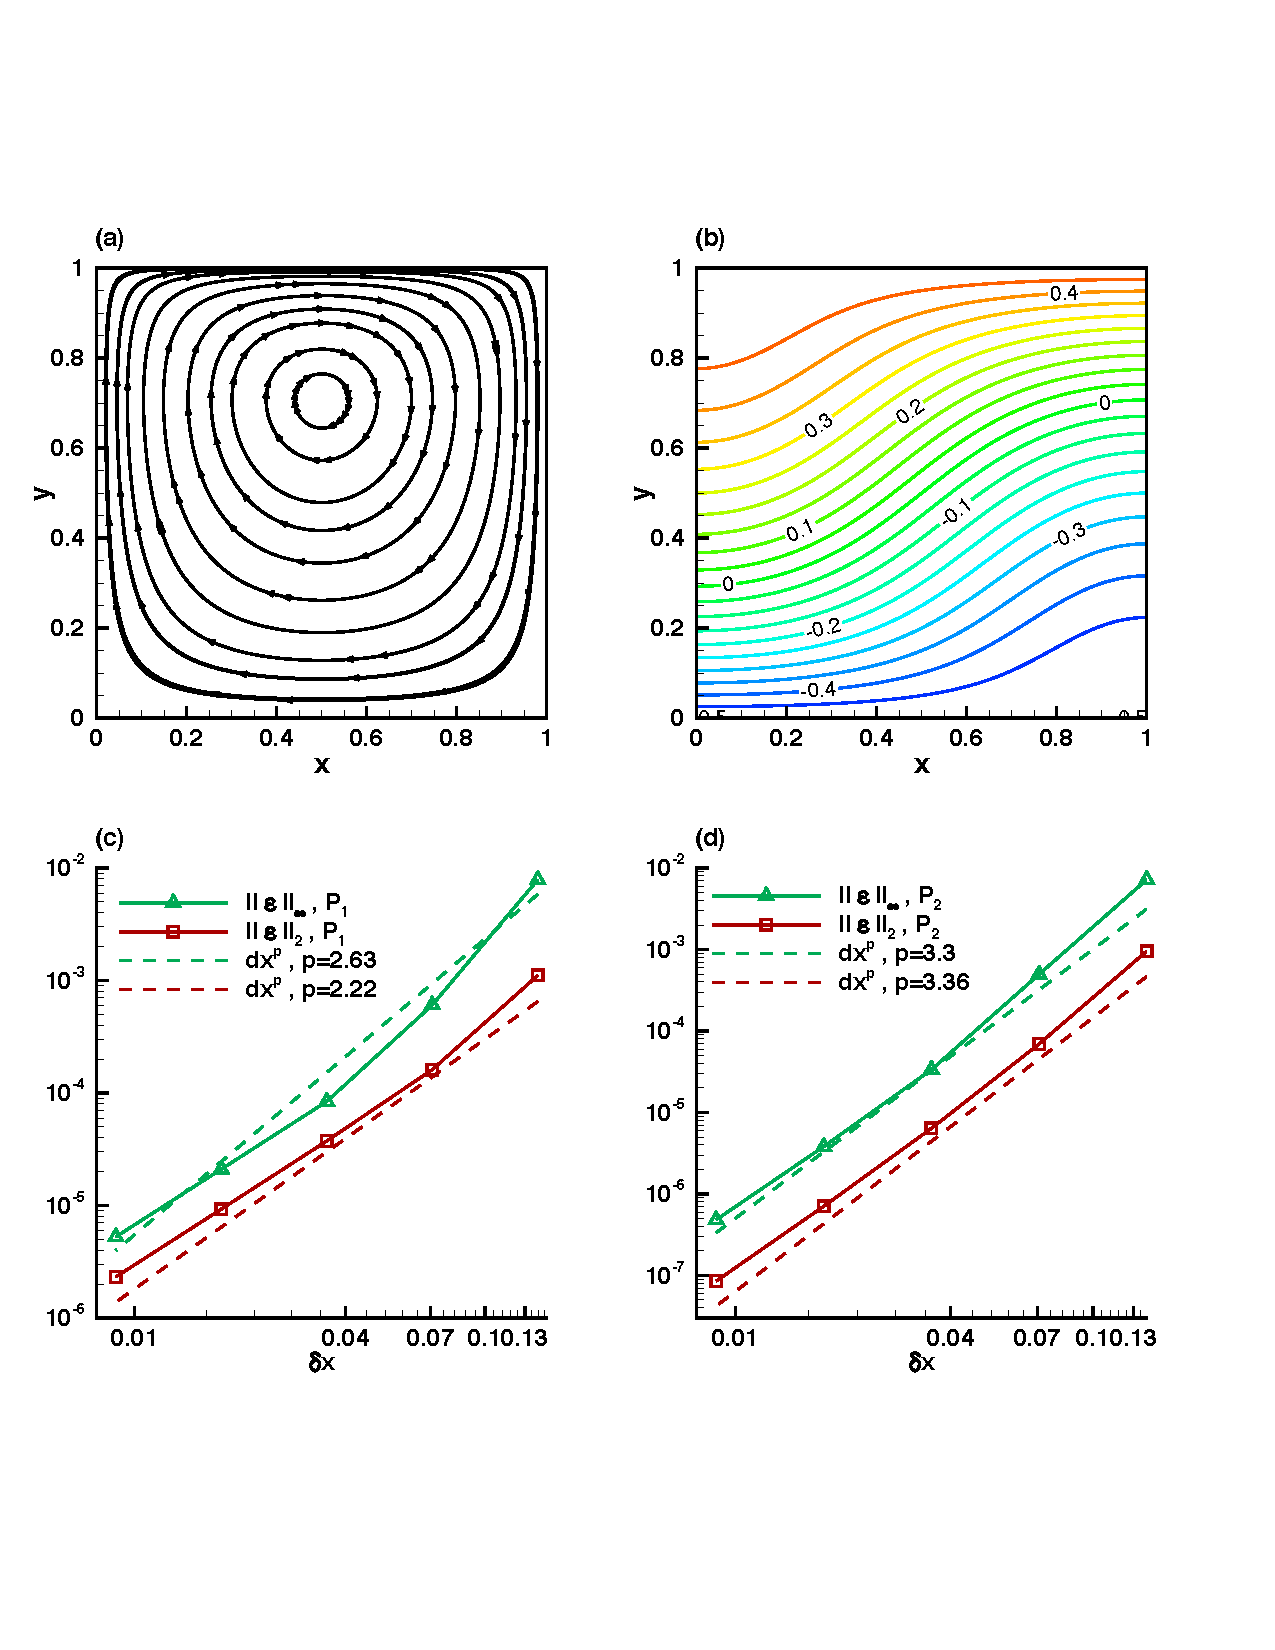
\includegraphics[width=\textwidth]{\figpath/Fig_cap_2/figsCPC_03} 
	\end{center}
	\caption{Burggraf stationary flow with thermal effects used to test the space accuracy of the numerical scheme. Streamlines (a) and temperature contours (b) of the flow field.	
Global error $\varepsilon$ (cf. Eq. (\ref{eq-epsconv})) for  the temperature: (c) P$_1$ and (d) P$_2$ finite elements.}
	\label{fig-conv-burggraf}
\end{figure}

%\pagebreak
%%%%%%%%%%%%%%%%%%%%%%%%%%%%%%%%%%%%%%%%%%%
\section{Time accuracy: manufactured unsteady solution} \label{subsub-conv-nourg}

To test the time accuracy of the Gear (BDF2) scheme, we used the manufactured time-dependent solution suggested in \cite{nourgaliev2016fully}:
\begin{align}
\label{eq-manufN}
	u_1(x,y,t) &=& \left( \delta U_0 + \alpha_u \, \sin(t) \right) \, \cos(x+ \gamma_1 t) \, \sin(y+ \gamma_2 t), \\ \nonumber
	u_2(x,y,t) &=& - \left( \delta U_0 + \alpha_u \sin(t) \right) \, \sin(x+ \gamma_1 t) \, \cos(y+ \gamma_2 t), \\ \nonumber
	T(x,y,t) &=& \bar{T} + \left( \delta T_0 + \alpha_t \sin(t) \right) \, \cos(x+ \gamma_1 t) \, \sin(y+ \gamma_2 t), \\ \nonumber
	p(x,y,t) &=& \bar{P} + \left(\delta P_0 + \alpha_p \sin(t) \right) \, \sin(x+ \gamma_1 t) \, \cos(y+ \gamma_2 t), 
\end{align}
The values of the constants are reported in Table \ref{tab-constant}.
\begin{table}[!h]
\centering
\begin{tabular}{*{10}{c}}
 % \toprule
  $\gamma_1$ & $\gamma_2$ & $\bar{P}$ & $\bar{T}$ & $\delta P_0$ & $\delta T_0$ & $\delta U_0$ & $\alpha_p$ & $\alpha_u$ & $\alpha_t$\\
   \midrule
  $0.1$ & $0.1$ & $0$ & $1.0$ &  $0.1$ & $1.0$ & $1.0$ & $0.05$ & $0.4$ & $0.1$ \\
 % \bottomrule
 \end{tabular}
\caption{Parameter for the time-dependent manufactured solution (\ref{eq-manufN}).}
\label{tab-constant}
\end{table}
The corresponding forcing source terms are:
\begin{eqnarray}
	f_{u_1} &=& \alpha_u \, \cos(t) \, \cos(a) \sin(b) - U_c \, \gamma_1 \, \sin(a) \sin(b) + U_c \, \gamma_2  \, \cos(a)\cos(b) \\ \nonumber
	  & & - U_c \,  u_1(x,y,t) \, \sin(a) \sin(b) + U_c \,  u_2(x,y,t) \, \cos(a) \cos(b)
	  + P_c \, \cos(a) \cos(b)\\ \nonumber
	  & & + \frac{2}{Re} \, u_1(x,y,t), \\	  \nonumber
	f_{u_2} &=& - \alpha_u \,  \cos(t)  \, \sin(a) \cos(b) - U_c \,  \gamma_1  \,  \cos(a) \cos(b) + U_c \,  \gamma_2 \,  \sin(a)\sin(b) \\ \nonumber
		  & & - U_c \,  u_1(x,y,t)  \,  \cos(a) \cos(b) + U_c  \, u_2(x,y,t)  \,  \sin(a) \sin(b)
		  -  P_c  \,  \sin(a)  \,  \sin(b)\\ \nonumber
		  & &+ \frac{2}{Re} \,  u_2(x,y,t)
		  - \frac{Ra}{Pr Re^2} \,  T(x,y,t), \\  \nonumber
	f_{T} &=& \alpha_t \,  \cos(t) \,  \cos(a) \sin(b) -  T_c  \,  \gamma_1 \,  \sin(a) \sin(b) + T_c \,   \gamma_2  \,  \cos(a)\cos(b) \\ \nonumber
		  & &-  T_c \,  u_1(x,y,t)  \,  \sin(a) \sin(b)  
		  +   T_c  \,  u_2(x,y,t)  \, \cos(a) \cos(b) 
		  + \frac{2 K}{Re Pr} \,  T_c  \, \cos(a) \sin(b), \\ \nonumber
\end{eqnarray}
where $a = (x+ \gamma_1 t), \,
b = (y+ \gamma_2 t)$ and  
$U_c = (\delta U_0 + \alpha_u \sin(t)), \,
	T_c = (\delta T_0 + \alpha_u \sin(t)), \,
	P_c = (\delta P_0 + \alpha_u \sin(t))$.

Guided by  the results obtained  in \S \ref{subsub-conv-burg} for the space accuracy, we fixed the grid size to $h=dx = 0.01$ to ensure small spatial discretization errors.
For diminishing values of the time step $\delta t$, the solution was evolved in time up to the time instant $t_{max} = \pi$ at which the error  (\ref{eq-epsconv}) was computed. 
The time convergence is displayed in Figure \ref{fig-conv-bdf2} for the temperature variable. 
The expected second order convergence in time is obtained for both P$_1$ (Figure \ref{fig-conv-bdf2}a) and P$_2$ (Figure \ref{fig-conv-bdf2}b) discretizations of the temperature.

\begin{figure}[!h]
	\begin{center}
		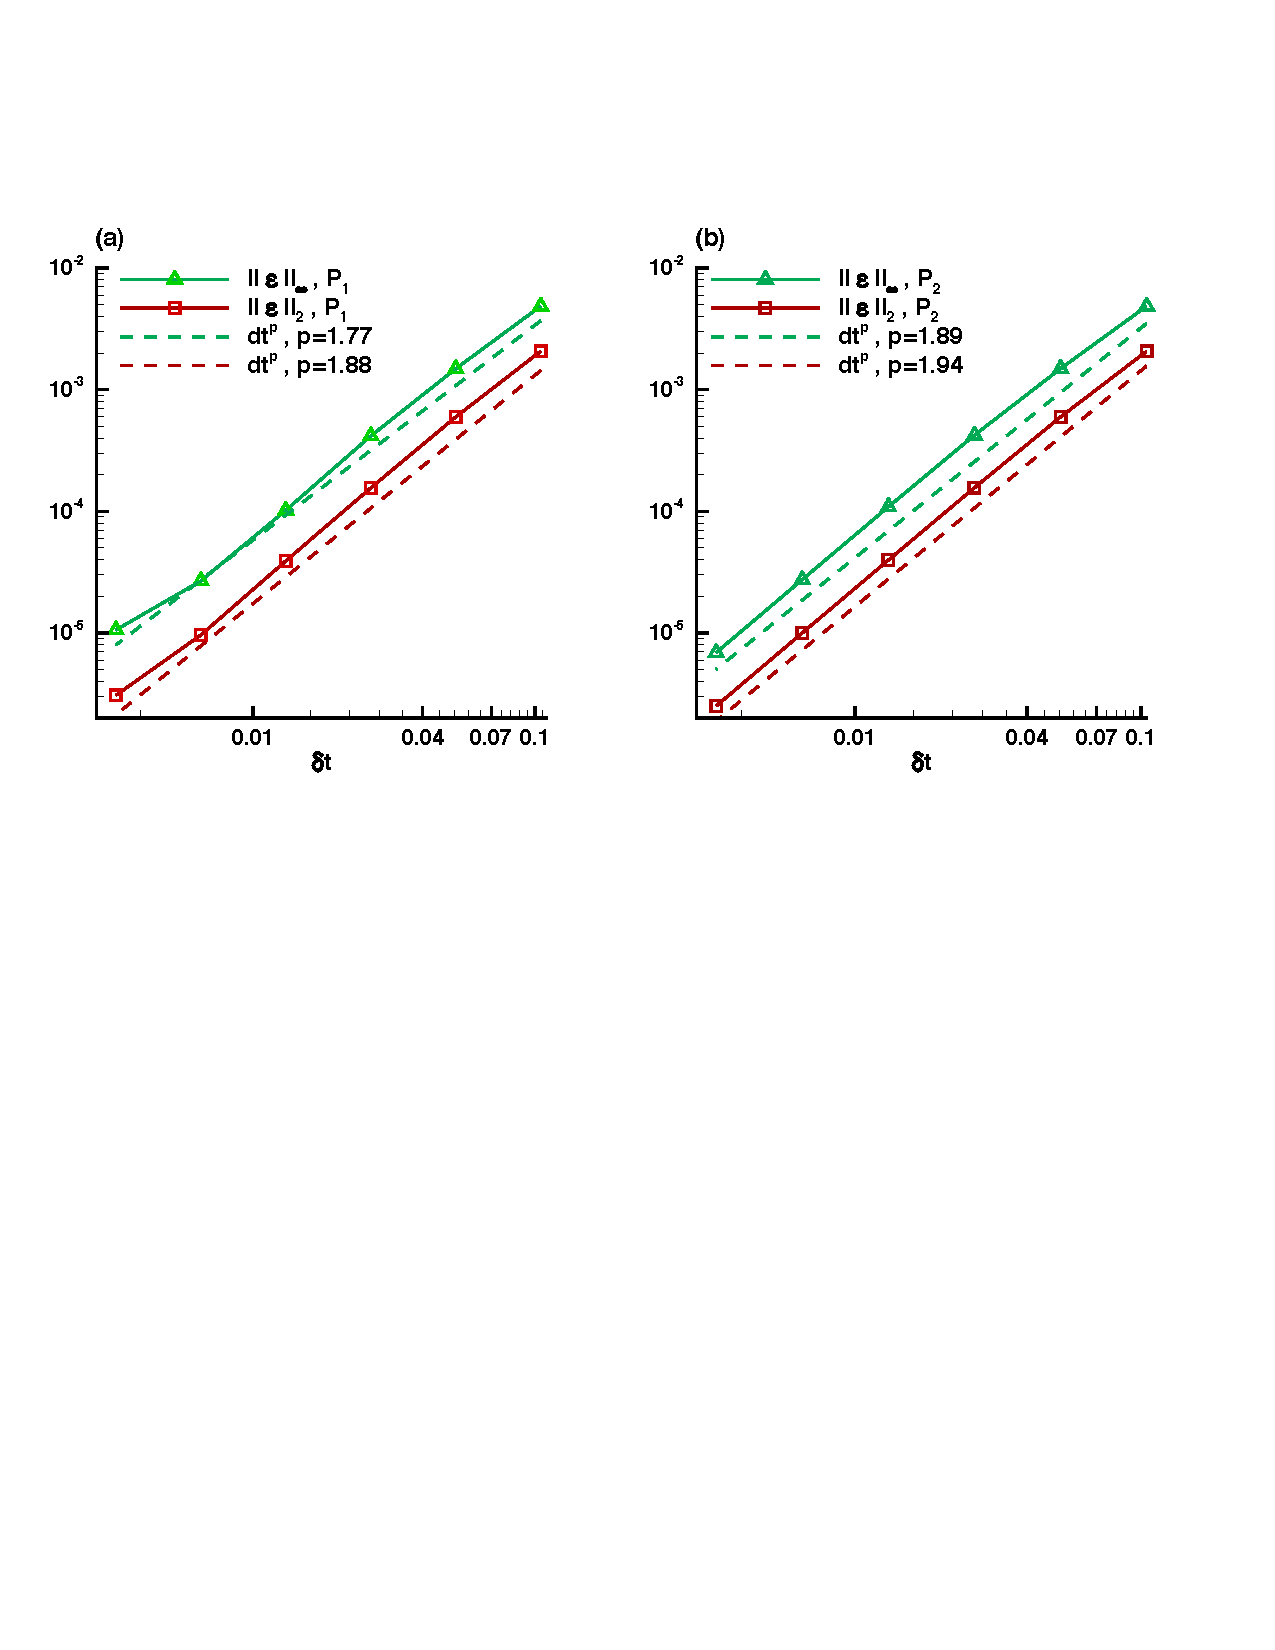
\includegraphics[width=\textwidth]{\figpath/Fig_cap_2/figsCPC_04} 
	\end{center}
	\caption{Time accuracy of the numerical scheme tested using the time-dependent manufactured solution of \cite{nourgaliev2016fully}. Evolution of the global error $\varepsilon$ given in (\ref{eq-epsconv}) for  the temperature at $t_{max} = \pi$. Discretizations using: (a) P$_1$ and (b) P$_2$ finite elements.}
	\label{fig-conv-bdf2}
\end{figure}


%\section{Accuracy and convergence} \label{subsec-conv}
%We test the accuracy of our numerical method in this section.
%Both space and time convergence orders are demonstrated by using the Burggraf flow and a manufactured solution defined by \cite{nourgaliev2016fully} for the incompressible Navier-Stokes equations.
%The global error $ \| \varepsilon_h \|$ is defined as follows:
%
%\begin{equation}
%  \| \varepsilon_h \| = \| \Phi_e - \phi_h \|,
%\end{equation}
%where $\Phi_e$ is the exact solution and $\phi_h$ is the numerical solution.
%Thus, by computing $\| \varepsilon_h \|$ for either different grids or different time steps, one can evaluate the convergence order $p$, since it is represented by the slope of the corresponding curve in logarithmic coordinates.
%
%Computations are done for the convection of air, with a Rayleigh number $Ra = 10^6$ and a Prandtl number $Pr = 0.71$.
%
%\subsection{Burggraf flow} \label{subsub-conv-burg}
%
%\begin{figure}
%	\begin{center}
%		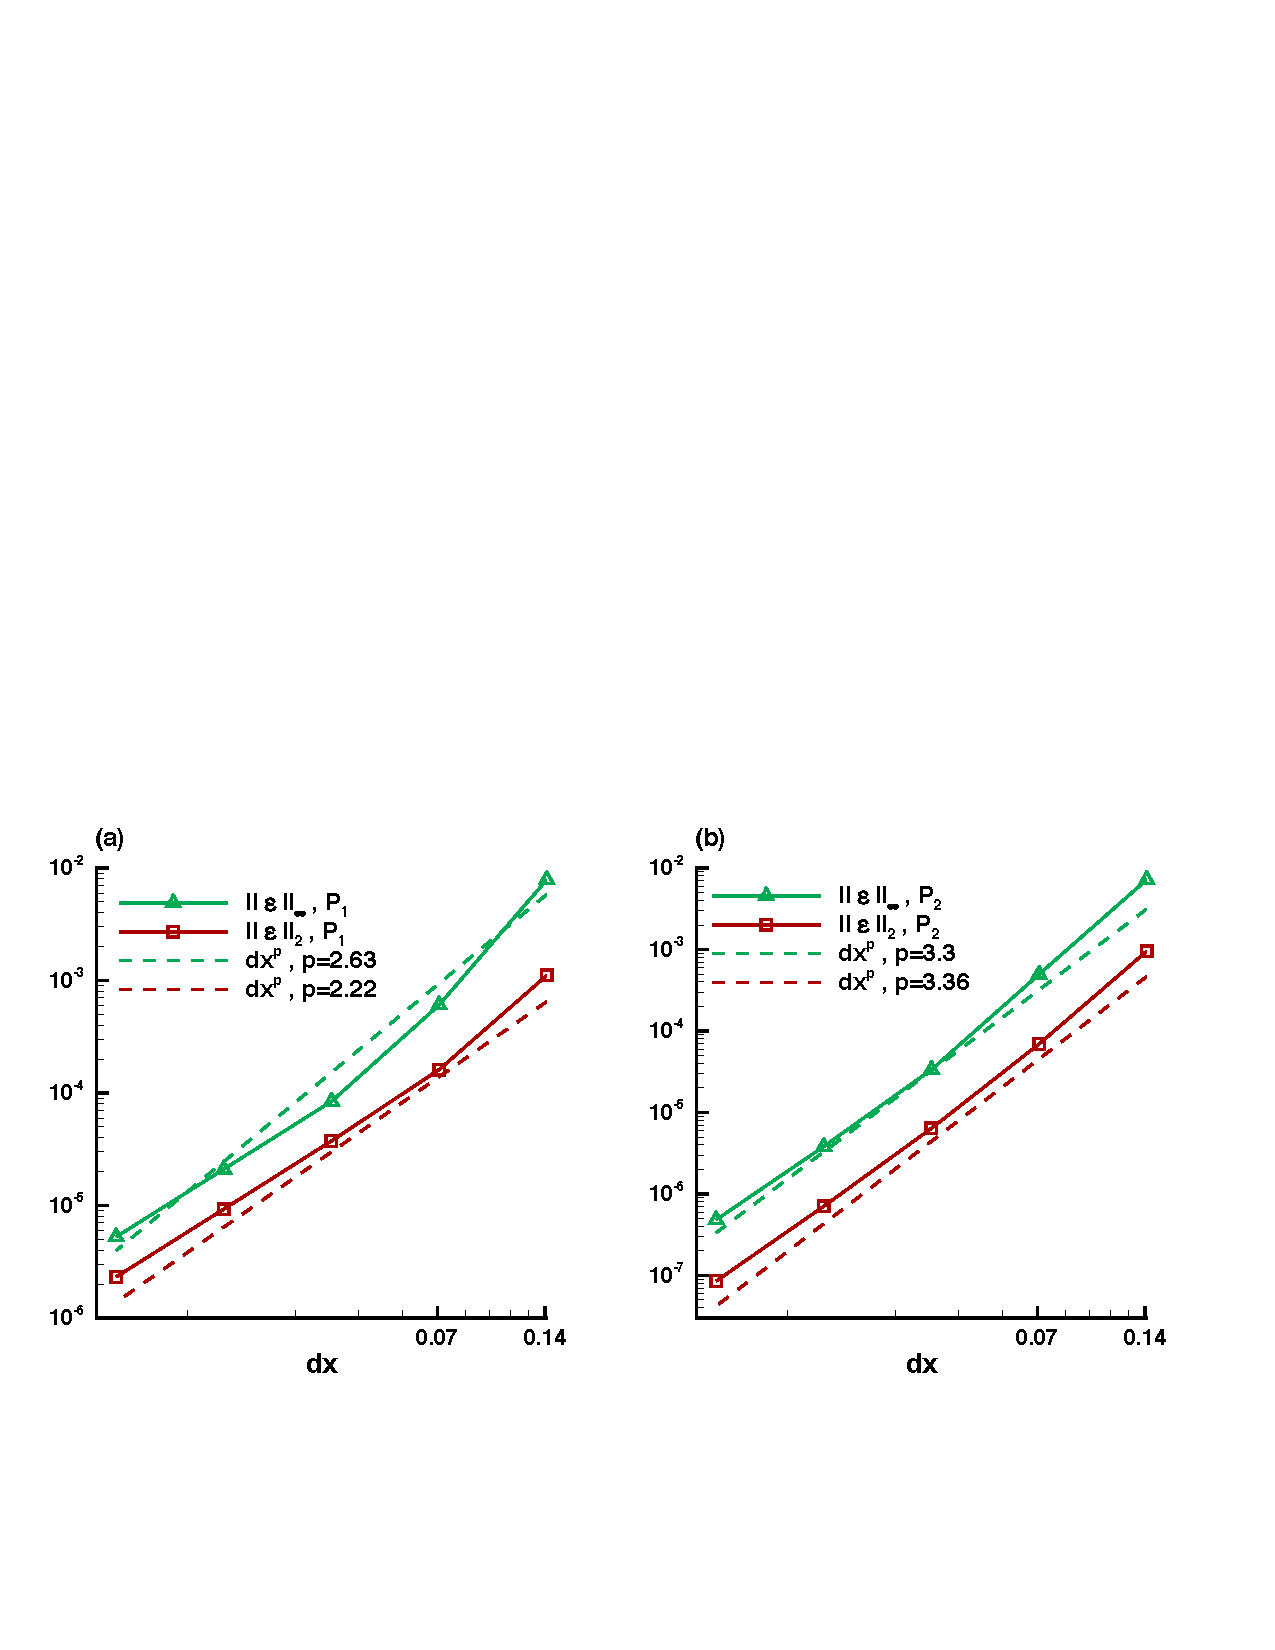
\includegraphics[width=0.98\textwidth]{\figpath/Fig_cap_2/Convergence_BURGGRAF} 
%	\end{center}
%	\caption{Burggraf flow. Evolution of the global error $\| \varepsilon_h \|$ for both $\mathcal{L}_2$-norm and $\mathcal{L}_\infty$-norm, with different grid size. A Taylor-Hood finite element (P$_2$ for velocity and P$_1$ for pressure) is used for space discretization by taking either P$_1$ finite element (a) or P$_2$ finite element (b) for the temperature field.}
%	\label{fig-conv-burggraf}
%\end{figure}
%
%To demonstrate the space accuracy of our method, we compute the well-known analytical solution called the Burggraf flow.
%It consists of a steady recirculating flow in a square cavity $[ 0 , 1] \times [ 0 , 1]$, with a moving wall at the top boundary and non-slip wall conditions at the others :
%
%\begin{eqnarray}
%   u(x,0) &=& u(0,y) = u(1,y) = 0, \\
%   u(x,1) &=& \sigma (x^4 - 2x^3 + x^2).
%\end{eqnarray}
%Besides, constant temperatures are imposed at the top and the bottom walls, while others are assumed to be adiabatic.
%The exact solution of the flow is:
%\begin{eqnarray}
%   u1(x,y) &=& \sigma g'(x) h'(y), \\\nonumber
%   u2(x,y) &=& - \sigma g''(x) h(y), \\\nonumber
%   p(x,y)   &=& \frac{\sigma}{Re} \left( h^{(3)}(y) g(x) + g''(x)h'(y) \right) + \frac{\sigma}{2} g'(x)^2 \left( h(y)h''(y)-h'(y)^2 \right),\\ \nonumber
%   T(x,y) &=& T_{c} + (T_{h} - T_{c}) y + a(x) b(y), \\ \nonumber
%\end{eqnarray}
%with,
%\begin{eqnarray}
%   g(x) &=& \frac{x^5}{5} - \frac{x^4}{2} - \frac{x^3}{3}, \\ \nonumber
%   h(y) &=& y^4 - y^2, \\ \nonumber
%   a(x) &=& \cos (\pi x), \\ \nonumber
%   b(x) &=& y(1-y).
%\end{eqnarray}
%Hence, forcing term are defined as follows:
%
%\begin{eqnarray}
%   f_{u1} &=& 0 \\ \nonumber
%   f_{u2} &=& \sigma^2 h(y) h'(y) \left( g''(x)^2 - g'(x)g^{(3)}(x) \right) \\ \nonumber
%   &+& \frac{\sigma}{Re}\left( g^{(4)}(x) h(y) + 2 g''(x)h''(y) + g(x) h^{(4)}(y) \right) \\ \nonumber
%   &+& \frac{\sigma^2}{2} g'(x)^2 \left( h(y) h^{(3)}(y) - h'(y)h''(y) \right) - \frac{Ra}{Pr Re^2} T(x,y),\\ \nonumber
%   f_T &=& u1(x,y) a'(x) b(y) + u2(x,y) \left( T_h - T_c + a(x) b'(y) \right) \\ \nonumber
%   &-& \frac{K}{Re Pr} \left( a''(x)b(y) + a(x) b''(y) \right).
%\end{eqnarray}
%We use the Taylor-Hood finite element (P$_2$ for velocity and P$_1$ for pressure) for the space discretization with either P$_1$ or P$_2$ finite element for the temperature field.
%Figure \ref{fig-conv-burggraf} plots the decrease of the global discretization error $\| \varepsilon_h \|$ for both $\mathcal{L}_2$-norm and $\mathcal{L}_\infty$-norm function of the grid size.
%The expected second order convergence is obtained with a P$_1$ finite element for the temperature (Figure \ref{fig-conv-burggraf}a), and even a nearly third order is noticed with a P$_2$ finite element on the temperature (Figure \ref{fig-conv-burggraf}b).
%
%\subsection{Manufactured solution} \label{subsub-conv-nourg}
%\begin{figure}
%	\begin{center}
%		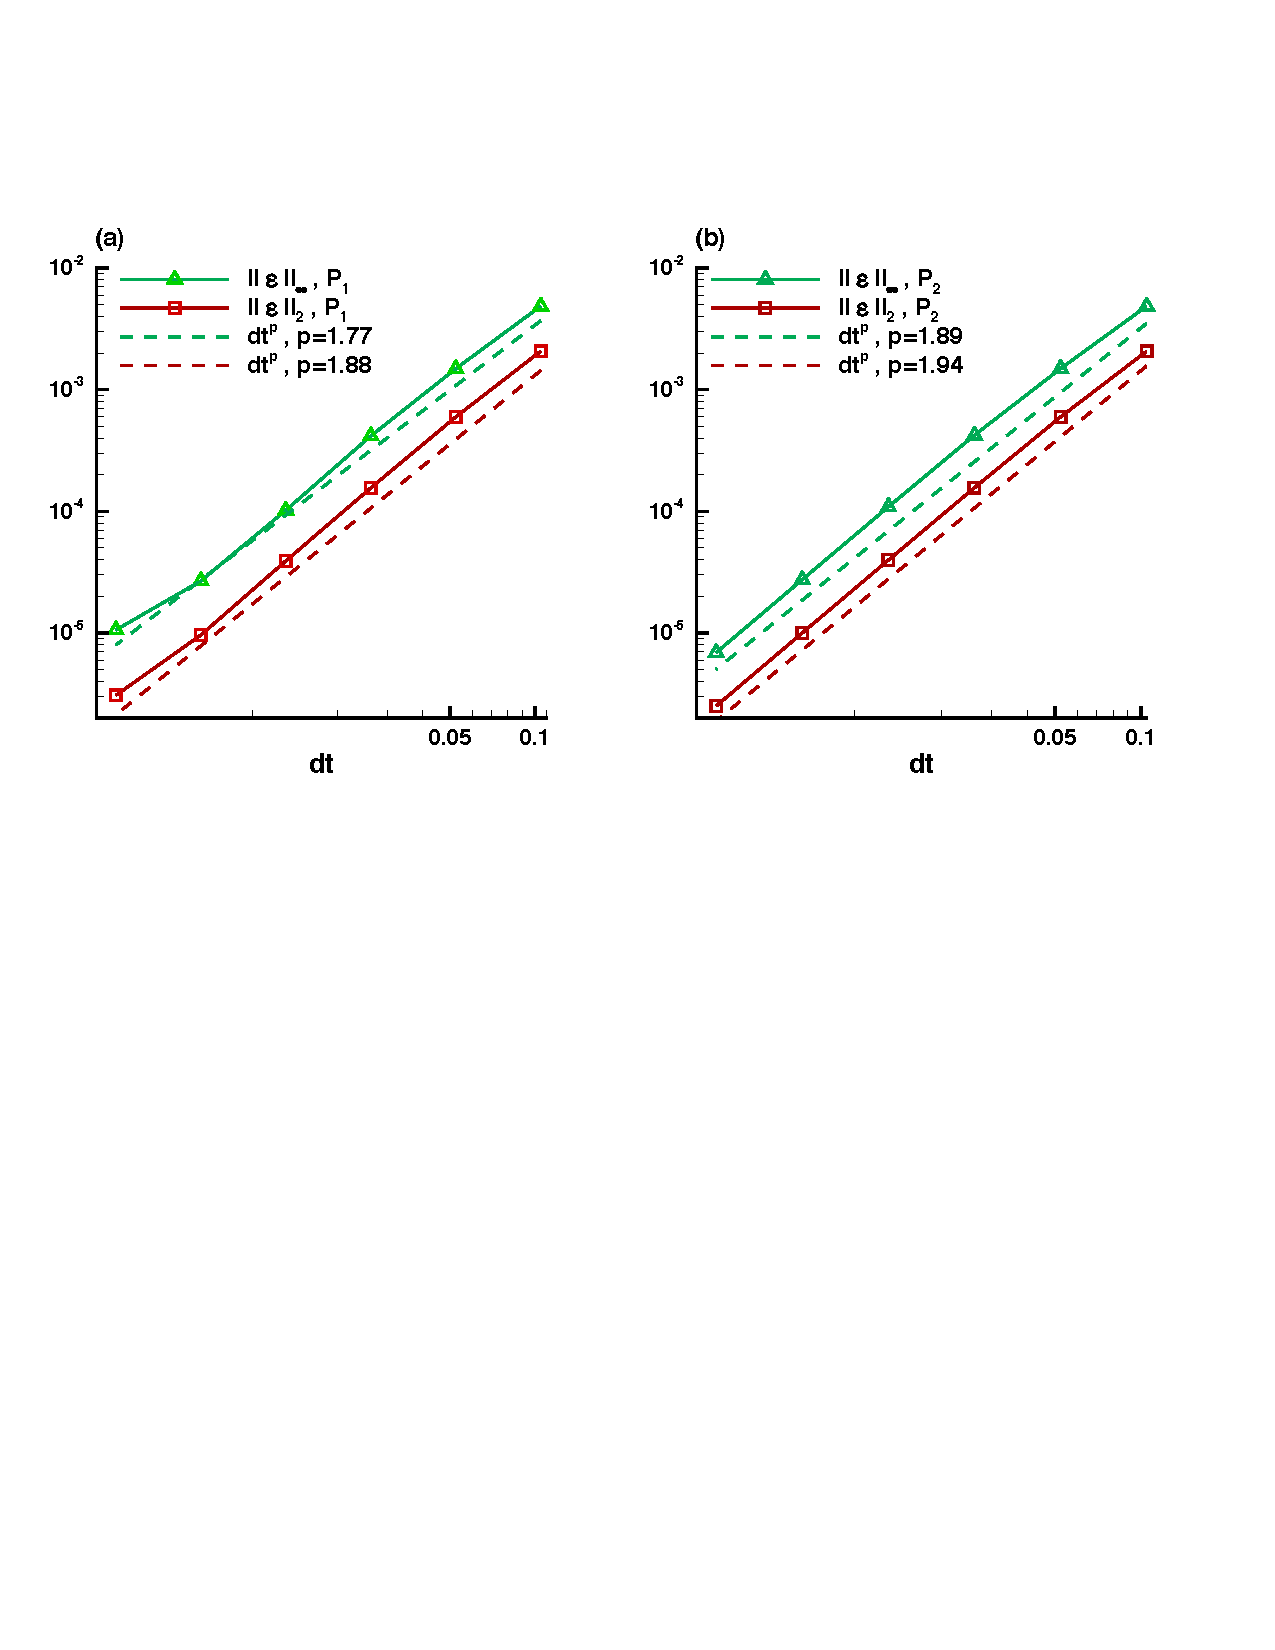
\includegraphics[width=0.98\textwidth]{\figpath/Fig_cap_2/Convergence_BDF2} 
%	\end{center}
%	\caption{Manufactured solution of \cite{nourgaliev2016fully} for unsteady incompressible Navier-Stokes equation at dimensionless time $t = \pi$. Evolution of the global error $\| \varepsilon_h \|$ for both $\mathcal{L}_2$-norm and $\mathcal{L}_\infty$-norm, with different time steps, with a P$_1$ finite element (a) and a P$_2$ finite element (b) for the temperature.}
%	\label{fig-conv-bdf2}
%\end{figure}
%
%The time integration is based on the implicit second order scheme BDF2.
%We use the manufactured solution of \cite{nourgaliev2016fully} to measure the temporal convergence order.
%\begin{eqnarray}
%	u_1(x,y,t) &=& \left( \delta U_0 + \alpha_u \, \sin(t) \right) \, \cos(x+ \gamma_1 t) \, \sin(y+ \gamma_2 t), \\ \nonumber
%	u_2(x,y,t) &=& - \left( \delta U_0 + \alpha_u \sin(t) \right) \, \sin(x+ \gamma_1 t) \, \cos(y+ \gamma_2 t), \\ \nonumber
%	T(x,y,t) &=& \bar{T} + \left( \delta T_0 + \alpha_t \sin(t) \right) \, \cos(x+ \gamma_1 t) \, \sin(y+ \gamma_2 t), \\ \nonumber
%	p(x,y,t) &=& \bar{P} + \left(\delta P_0 + \alpha_p \sin(t) \right) \, \sin(x+ \gamma_1 t) \, \cos(y+ \gamma_2 t), 
%\end{eqnarray}
%The value of the constants are reported on Table \ref{tab-constant}.
%\begin{table}[!h]
%\centering
%\begin{tabular}{*{10}{c}}
% % \toprule
%  $\gamma_1$ & $\gamma_2$ & $\bar{P}$ & $\bar{T}$ & $\delta P_0$ & $\delta T_0$ & $\delta U_0$ & $\alpha_p$ & $\alpha_u$ & $\alpha_t$\\
%   \midrule
%  $0.1$ & $0.1$ & $0$ & $1.0$ &  $0.1$ & $1.0$ & $1.0$ & $0.05$ & $0.4$ & $0.1$ \\
% % \bottomrule
%
% \end{tabular}
%\caption{Parameter for the manufactured solution.}
%\label{tab-constant}
%\end{table}
%
%\noindent Thus, forcing terms are:
%
%\begin{eqnarray}
%	f_x &=& \alpha_u \, \cos(t) \, \cos(a) \sin(b) - U_c \, \gamma_1 \, \sin(a) \sin(b) + U_c \, \gamma_2  \, \cos(a)\cos(b) \\ \nonumber
%	  & & - U_c \,  u_1(x,y,t) \, \sin(a) \sin(b) + U_c \,  u_2(x,y,t) \, \cos(a) \cos(b)
%	  + P_c \, \cos(a) \cos(b)\\ \nonumber
%	  & & + \frac{1}{Re} \, u(x,y,t), \\	  \nonumber
%	f_y &=& - \alpha_u \,  \cos(t)  \, \sin(a) \cos(b) - U_c \,  \gamma_1  \,  \cos(a) \cos(b) + U_c \,  \gamma_2 \,  \sin(a)\sin(b) \\ \nonumber
%		  & & - U_c \,  u_1(x,y,t)  \,  \cos(a) \cos(b) + U_c  \, u_2(x,y,t)  \,  \sin(a) \sin(b)
%		  -  P_c  \,  \sin(a)  \,  \sin(b)\\ \nonumber
%		  & & -\frac{1}{Re} \,  v(x,y,t)
%		  - \frac{Ra}{Pr Re^2} \,  T(x,y,t), \\  \nonumber
%	f_{\theta} &=& \alpha_t \,  \cos(t) \,  \cos(a) \sin(b) -  T_c  \,  \gamma_1 \,  \sin(a) \sin(b) + T_c \,   \gamma_2  \,  \cos(a)\cos(b) \\ \nonumber
%		  & &-  T_c \,  u_1(x,y,t)  \,  \sin(a) \sin(b)  
%		  +   T_c  \,  u_2(x,y,t)  \, \cos(a) \cos(b) 
%		  + \frac{K}{Re Pr} \,  T_c  \, \cos(a) \sin(b), \\ \nonumber
%\end{eqnarray}
%
%with: 
%$	U_c = (\delta U_0 + \alpha_u \sin(t)), \,
%	T_c = (\delta T_0 + \alpha_u \sin(t)), \,
%	P_c = (\delta P_0 + \alpha_u \sin(t)), $ \\
%and $	a = (x+ \gamma_1 t), \,
%	b = (y+ \gamma_2 t). \\$
%
%Since the space convergence rate was evaluated in \S \ref{subsub-conv-burg}, we fixe the grid size to $dx = 0.01$ to ensure a small spatial discretization errors, and we vary decreasingly the time step.
%Time convergence is displayed in Figure \ref{fig-conv-bdf2}. 
%The evolution of the global error with different time steps is plotted for both  $\mathcal{L}_2$-norm (red line) and $\mathcal{L}_\infty$-norm (green line), and the expected second order convergence is exposed for both P$_1$ (Figure \ref{fig-conv-bdf2}a) and P$_2$ (Figure \ref{fig-conv-bdf2}b) finite element for the temperature.

%\newpage
%\section{A finite-element toolbox for the simulation of phase-change systems with natural convection}\label{sec-desc-prog}
%
%The methods described previously were implemented in a 2D toolbox based on \ff software.
%%Using two input files, the toolbox offers to the user the choice between three scalings in order to compute different physical systems involving natural convection flow, ranging from natural convection of air and water to melting and solidification cycle of PCM or water freezing.
%%The solutions can be saved at recurrent iterations defined by the user beforehand, allowing later to restart the computation from  saved solutions.
%In this section we first describe the architecture of the programs and the organisation of files.
%Then we focus on the list of input parameters and the structure of output files.
%%
%\begin{figure}[!h]
%	\begin{center}
%		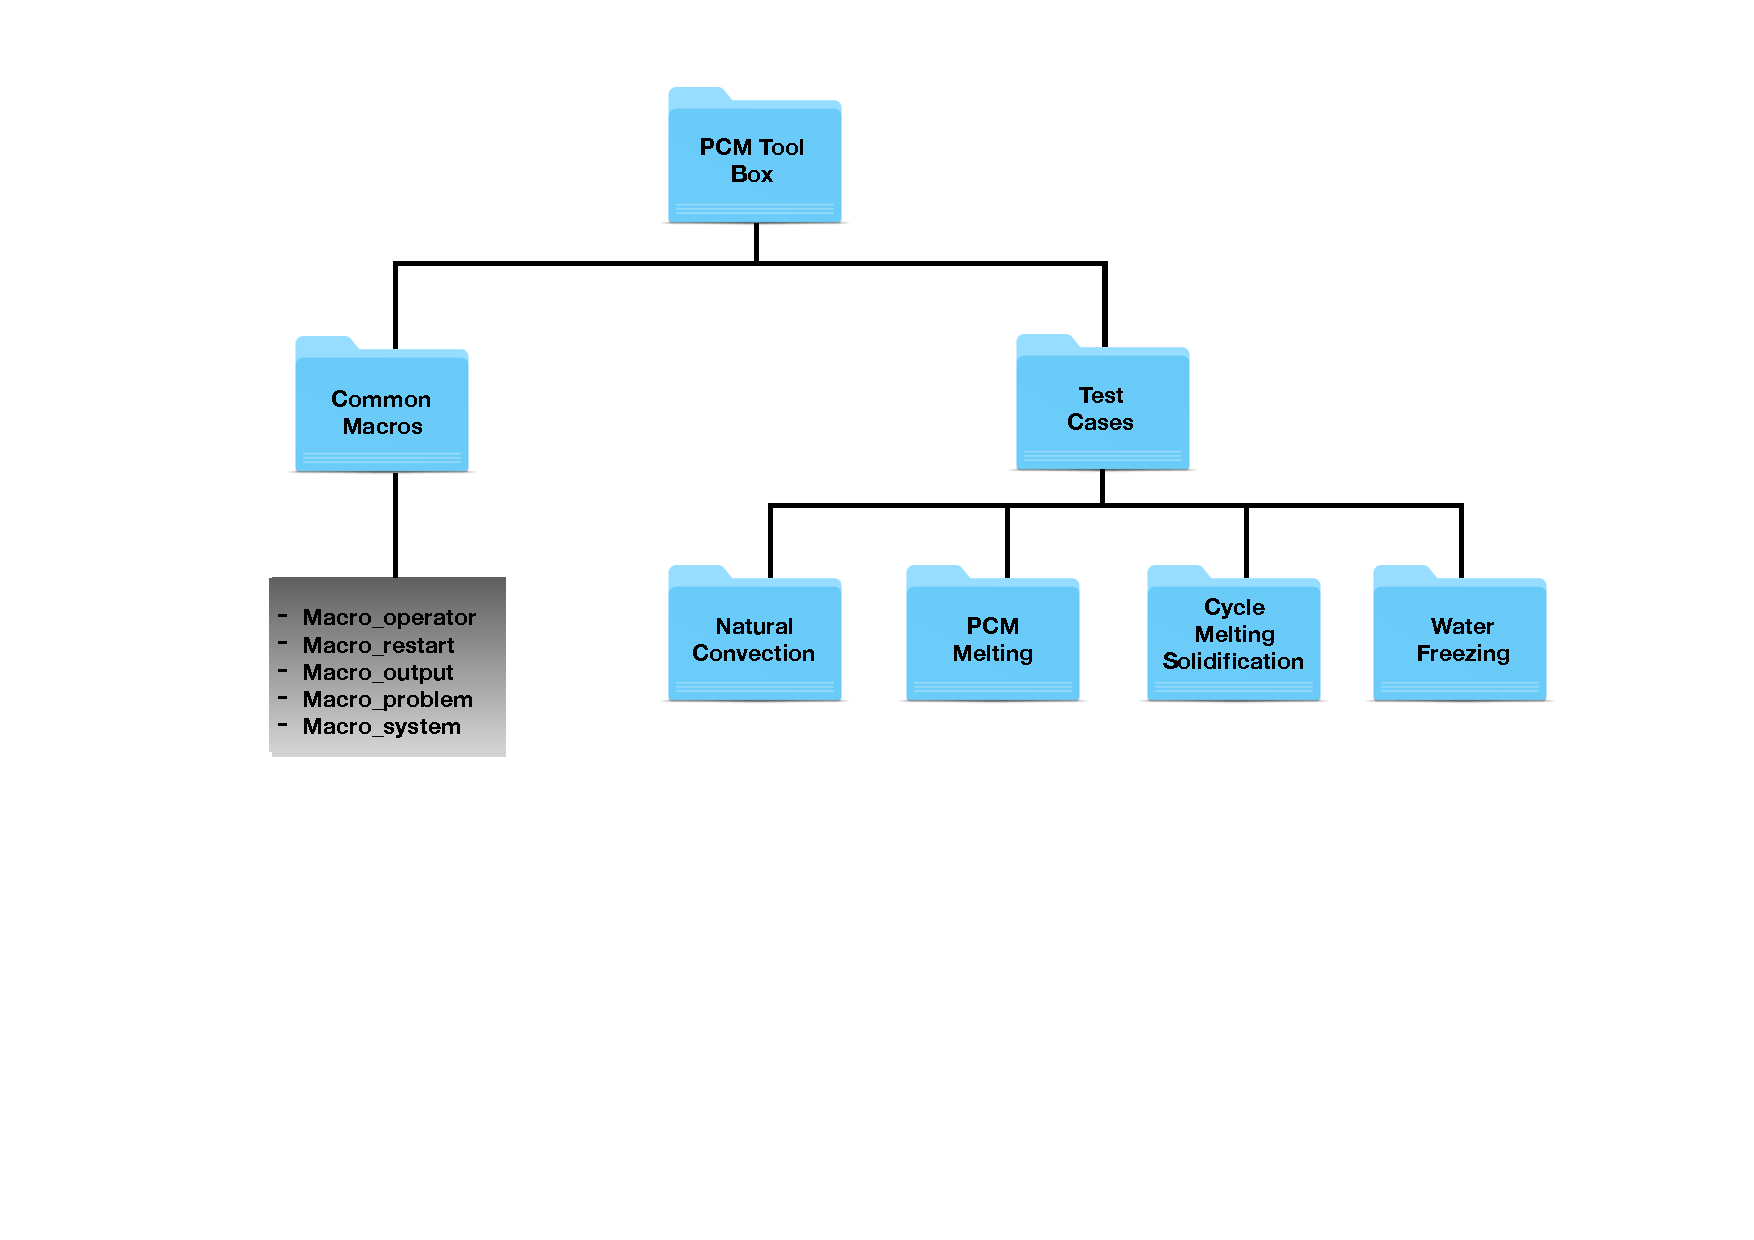
\includegraphics[width=0.9\textwidth]{\figpath/Fig_cap_2/FOLDER_arbor_3}
%	\end{center}
%	\caption{Folder tree structure of the FreeFem++ toolbox to solve phase change problems. Test cases and common macros are separated into two folders.}
%	\label{fig-folder-tree}
%\end{figure}
%
%\subsection{Program architecture}
%Figure \ref{fig-folder-tree} gives a schematic overview of the content of the toolbox. All files are provided in a directory called \texttt{PCM-Toolbox}.  Many detailed comments are included in the programs, with direct link to the mathematical expressions used in the paper. The used \ff syntax was intentionally kept at a low level of technicality and supplemented with detailed comments when specific more technical syntax was used.
%
%This directory is organized as follows:
%\begin{enumerate}
%   \item The directory \texttt{Common-Macros} contains five files:\\
%$\bullet$ {\em Macro$\_$operator.idp} includes macros and functions defining mathematical operators,\\
%$\bullet$ {\em Macro$\_$problem.idp}: macros defining the variational formulation of the problem,\\
%$\bullet$ {\em Macro$\_$restart.idp}: macros used to start a new simulation from a saved field,\\
%$\bullet$ {\em Macro$\_$output.idp}: macros used to save the solution with different formats,\\
%$\bullet$ {\em Macro$\_$system.idp}: macros identifying the OS and defining specific OS-commands.
%
%   \item The directory \texttt{Test-Cases}  contains four subdirectories, each of them defining one of the following applications:\\
%    $\bullet$  natural convection of air or water in a differentially heated square cavity, \\
%    $\bullet$  melting of a PCM stored in containers of different shapes,\\
%    $\bullet$  melting followed by solidification of a rectangular PCM,\\
%    $\bullet$  freezing of pure water in a square cavity.\\
%   Each subdirectory contains  three files: {\em NEWTON$\_$\$case.edp} is the main \ff script file, $param_\_phys.inc$ defines the physical parameters and $param_\_num.inc$ the numerical parameters. For example, to run the natural convection case of air in a square cavity, the user can use the following command in a terminal window:
%  \texttt{FreeFem++ NEWTON$\_$stat$\_$natconv.edp}.\\
%  The folder structure of each test case is illustrated in Figure \ref{fig-case-folder}.
%  The obtained solutions are saved in the folder \texttt{OUTPUT/Data}. Depending on the output format selected by the user,  data files are generated in specific folders for being visualized with: Tecplot, Paraview, Gnuplot or Medit. We also provide in the folder \texttt{Figures} ready-made layouts for these visualisation softwares. The user can thus obtain the figures from this paper using  newly generated data. More details about the output structure are given below.
%\end{enumerate}
%
%\begin{figure}[!h]
%	\begin{center}
%		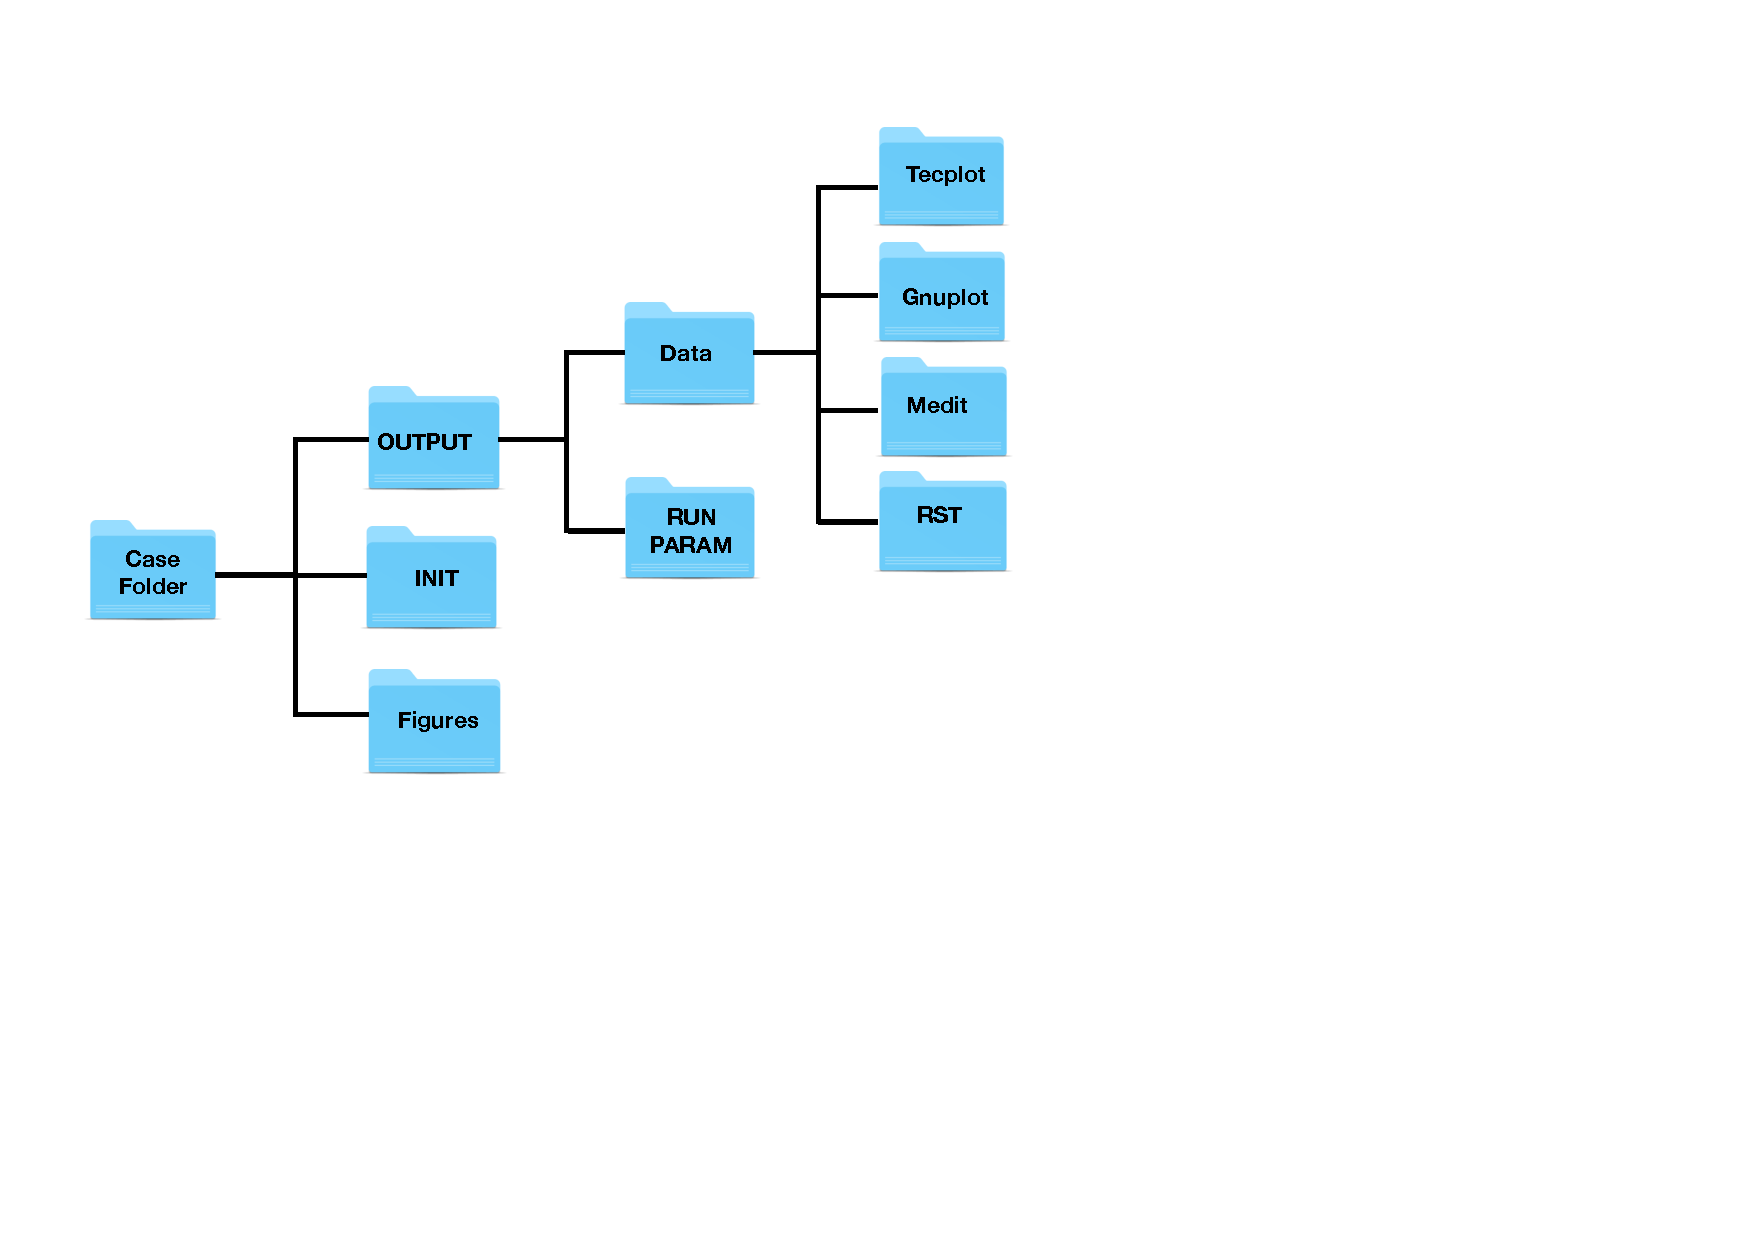
\includegraphics[width=0.7\textwidth]{\figpath/Fig_cap_2/figsCPC_02}
%	\end{center}
%	\caption{Structure of each Test-case folder. 
%	}
%	\label{fig-case-folder}
%\end{figure}
%
%\subsection{Input parameters}
%
%Physical parameters and parameters related to the run are separated into two files.\\
%{\bf (1)} The file $param_\_phys.inc$ contains the physical descriptions of the problem:
%\begin{itemize}
%   \item {\bf typeT}: is the finite-element type for the temperature, with possible values \texttt{P2} or \texttt{P1},
%   \item {\bf Torder}: is the accuracy order of the time integration scheme, with possible values $1$ (Euler scheme) or $2$ (Gear scheme),
%   \item {\bf scalAdim}: defines the characteristic scales of the problem, see (\ref{eq-adim}). Possible values 1, 2 or 3 correspond to the following choice of the characteristic scales \citep{dan-2014-JCP}:
%   \begin{eqnarray} \label{eq-scal1}
%    (1) &:&  V_\vref^{(1)} = \frac{\nu_l}{H} \Longrightarrow \ds t_\vref^{(1)} = \frac{H^2}{\nu_l}  \Longrightarrow \Rey=1,\\
%      \label{eq-scal2}
%     (2) &:& V_\vref^{(2)} = \frac{\alpha}{H} \Longrightarrow \ds t_\vref^{(2)} = t_\vref^{(1)} \Prd  \Longrightarrow \Rey =1/\Prd,\\
%      \label{eq-scal3}
%     (3) &:& V_\vref^{(3)} = \frac{\nu_l}{H} \sqrt{\frac{\Ray}{\Prd}} \Longrightarrow \ds t_\vref^{(3)} = t_\vref^{(1)} \sqrt{\frac{\Prd}{\Ray}}       \Longrightarrow \Rey = \sqrt{\frac{\Ray}{\Prd}},
%\end{eqnarray}
%   \item {\bf x$_l$, x$_r$, y$_l$, y$_r$}: are the values defining the dimensions of the cavity $[x_l,x_r]\times[y_l,y_r]$,
%   \item {\bf Pr, Ra, Ste}: are the  Prandtl, Rayleigh and Stefan numbers, see (\ref{eq-Rayleigh}) and (\ref{eq-RePr}),
%   \item {\bf T$_{hot}$, T$_{cold}$}: are  dimensionless temperatures according to (\ref{eq-adim}),
%   \item{\bf bcu$_1$, bcu$_2$, bcT}: are macros defining the velocity (u) and the temperature (T) boundary conditions.
%   \item {\bf epsi}: is the half width $\varepsilon$ of the mushy region. \underline{Default value} = $0.01$,
%   \item {\bf dt}: is the dimensionless time step,
%   \item {\bf t$_{max}$}: is the dimensionless final time,
%   \item {\bf Parameters for regularization functions}: \\
% The parameters of the hyperbolic-tangent function (\ref{eq-smooth}) used to regularize discontinuous functions are set by default as follows:
% \end{itemize}
%    \begin{table}[!ht]
%    \centering
%    \begin{tabular}{*{8}{c}}
%     & { f$_{s}$} & {f$_{l}$} & {a$_s$} & {$\theta_s$} & R$_s$ & {$\CKC$} & {b} \\
%       \toprule
%       {\it Enthalpy} & 0 & 1/Ste & 1 & 0.01 & 0.01  & - & - \\
%       \midrule
%       {\it Carman - Kozeny} & 0 & 1 & 1 & 0.01 & 0.01  & 10$^6$ & 10$^{-7}$ \\
%          \midrule
%       {\it Conductivity (water)} & 1 & 2.26/0.578 & 1 & $\theta_f$ & 0.015 & - & - \\
%       \bottomrule
%     \end{tabular}
%    \label{tab-constant}
%    \end{table}
%   \begin{itemize} 
%    \item {\bf rho(T) and Drho(T)}: (water cases only) define  the density and its derivative as functions of the temperature, following the model
%\citep{Gebhart1977}:\\
% 
%    \begin{table}[!ht]
%    \centering
%    \begin{tabular}{*{4}{c}}
%    	\multicolumn{4}{c}{
%      $\rho(T) = \rho_m (1 - \omega | T - T_m |^q),$}\\	\hline
%    $\rho_m$ [kg/m$^3$]  & $\omega$ [$^o$C$^{-q}$] & q & $T_m$  [$^o$C] \\
%       \toprule
%            $999.972$ & $9.2793 \cdot 10^{-6}$ & $1.894816$ & $4.0293$ \\
%       \bottomrule
%     \end{tabular}
%    \label{tab-rho}
%    \end{table}
%    \item {\bf f$_B$(T), df$_B$(T)}: define the buoyancy force and its derivative.
%    \end{itemize}
%
%\noindent {\bf (2)} The file {\em param$\_$num.inc} contains the parameters controlling the run.\\
%{\bf Restart parameters:}
%\begin{itemize}
%   \item {\bf Nsave}: the solution is saved every $N\!save$ time steps in the \texttt{Data} folder (see Figure \ref{fig-case-folder}). The temperature and the velocity fields are saved in \texttt{Tecplot} and \texttt{Medit} folders, while the liquid fraction, the Nusselt number, and the accumulated heat input are saved in the \texttt{Gnuplot} folder.
%   \item {\bf Nrestart}: restart files (mesh and solution) are saved every $N\!restart$ time steps. Solutions at current and previous iterations, the CPU time, the accumulated heat input $Q_0$, and the time step $dt$ are saved in the folder \texttt{RST}.
%   \item {\bf Ncondt}: allows the user to stop the run and save the solution properly. The file \texttt{OUTPUT/zz.condt} is read every $N\!condt$ time steps: if the user replaces the value "0" in this file by "1" the run is stopped. This is a simple solution for a clean stop of the job by the user. \underline{Default value} = $20$.
%   \item {\bf Nremesh}: the mesh is adapted every $N\!remesh$ iterations. If this parameter is set to "1" the mesh is adapted every time step.
%   \item {\bf IFrestart}: is a boolean controlling the set up of the initial field. \\
%  $I\!Frestart = 0$, the  initial condition is built in the code for each test case. For the PCM melting cases, the PCM is initially motionless at isothermal temperature. 
%  	To set-up a smooth initial field, a few time steps (with very small $\delta t$) are computed by increasing progressively the boundary temperature at the hot wall and the Rayleigh number (by continuation).  Outputs are saved in  \texttt{OUTPUT/Data-RST-0}.\\
%   $I\!Frestart > 0$, (positive integer values) the solution field previously computed at iteration $I\!Frestart$ is loaded from the folder \texttt{OUTPUT/Data-RST-filenameRST/RST}, with \texttt{filenameRST} a variable selecting the restart folder. \\
%   $I\!Frestart < 0$, (negative integer values), the same principle for loading a solution is used, but from the folder \texttt{INIT}  (see Figure \ref{fig-case-folder}). The solution fields stored in this folder could come from different previous calculations (\eg a steady state solution or, for the water, the natural convection field before freezing).
%\end{itemize}
%
%{\bf Newton parameters:}
%\begin{itemize}
%   \item {\bf epsconv}: is the value of  the stopping criterion for steady cases,
%   \item {\bf gamma}: is the penalty parameter in  (\ref{eq-time-disc1}). \underline{Default value} = $10^{-7}$,
%   \item {\bf tolNewton}: is the Newton tolerance $\xi_N$ (see (\ref{eq-Newton-algo})). \underline{Default value} = $10^{-6}$,
%   \item {\bf newtonMax}: limits the maximum number of iterations in  the Newton algorithm (\ref{eq-Newton-algo}). \underline{Default value} = $50$,
%  % \Blue{\item {\bf c$_1$, c$_2$, c$_3$}: \Red{(-- why not negative $a_2$ ?? si c'est trop compliqu� de changer, il faut le laisser tel quel --$>$ } \Blue{C'est modifi� en a$_2$ n�gatif maintenant dans le code)--}  are the coefficients of the time integration scheme: c$_1 =1/$dt, c$_2 = -1/$dt, c$_3 = 0$ correspond to the first order backward Euler scheme and c$_1 =1.5/$dt, c$_2 = -2/$dt, and c$_3 = 0.5/$dt to the second order Gear scheme.}
%\end{itemize}
%{\bf Mesh parameters:}
%\begin{itemize}
%   \item {\bf nbseg}: is  the number of segments for the discretisation along the $x$ and $y$ directions,
%   \item {\bf errh}: is the interpolation error level. \underline{Default value} = $0.02$,
%   \item {\bf hmin, hmax}: are the minimum and maximum edge size, respectively,
%   \item {\bf adaptratio}: is the ratio for a prescribed smoothing of the metric. For a value less than $1.1$ no smoothing is done. \underline{Default value} = $1.5$,
%   \item {\bf nbvx}: is the maximum number of vertices allowed in the mesh generator. \underline{Default value} = $50000$.
%\end{itemize}
%
%\noindent {\bf Output parameters:}
%   \begin{itemize}
%      \item {\bf dircase}: is the name of the output folder,
%      \item {\bf fcase}: is the prefix-name for ouput files.
%      \item {\bf Tecplot, Medit, Gnu}: correspond to the name of the visualisation software to be used; the format of the outputs written in \texttt{OUTPUT/Data} (see Figure \ref{fig-case-folder}) is accordingly set.  The files from the Tecplot folder can be easily read  also with Paraview.
%   \end{itemize}
%   
%\subsection{Outputs}
%When a computation starts, the \texttt{OUTPUT} directory is created (see Figure \ref{fig-case-folder})).
%It contains two folders storing the output data and the echo of the run parameters.
%The folder \texttt{Data} contains four subdirectories with different output format files of the computed solution. File names are created using  the prefix defined by the parameter {\bf fcase}, the current iteration and the current dimensionless time $t$. 
%Solution files can be visualized using either Tecplot or any other CFD Visualization tools (Paraview, Visit, etc.). 
%Moreover, {\em .gmsh}  (mesh) and {\em .rst} (fields) files are generated in the folder \texttt{RST} to enable restarts of the computation. Note that the folder \texttt{FFglut} contains  \ff scripts that re-read and visualize the RST-files to facilitate the selection of a restart field.  
%An {\em .echo} file with a summary of the main parameters, informations on the run and the names of the output files is saved in the folder \texttt{RUNPARAM}.  This directory additionally contains a copy of the {\em .inc} parameter files, allowing an easy identification of each case and preparing an eventual rerun of the same case.
%
%
%%Figure \ref{fig-folder-tree} gives a schematic overview of the content of the toolbox. All files are provided in a directory called {\it "PCM ToolBox FreeFem"}. 
%%This directory is organized as follows:
%%\begin{enumerate}
%%   \item the {\em Common Macros} directory contains four files:
%%   \begin{itemize}
%%      \item {\em Macro$\_$operator.idp} contains all macros and functions related to mathematical operators,
%%      \item {\em Macro$\_$restart.idp} contains the scripts to be used to take the computation back from saved solutions,
%%      \item {\em Macro$\_$output.idp} contains the scripts allowing to output the solutions,
%%      \item {\em Macro$\_$problem.idp} contains the variational formulation of the problem. 
%%   \end{itemize}
%%   \item The {\em Test Cases} directory contains four subdirectories clustering different physical test cases, including the natural convection of air or water in a differentially heated square cavity, the melting of a PCM included in various containers, the melting-solidification cycle of a PCM and finally the freezing of pure water in a square cavity. 
%%   For all cited cases, three files are given for each subdirectories: {\em NEWTON$\_$\$case.edp} the main FreeFem++ script file, $param_\_phys.inc$ the physical parameters and $param_\_num.inc$ the numerical parameters.
%%   The natural convection case can be launched, for example, using the following command line in a terminal window:\\
%%  {\em FreeFem++ NEWTON$\_$airconv.edp -nbseg 80}.\\
%%  This will run the natural convection of air using $80 \times 80$ grids.
%%\end{enumerate}
%%
%%\subsection{Input parameters}
%%We focus now on the description of the input parameters.
%%The physical parameters and parameters related to the run are separated into two files.\\
%%{\bf (1)} First, the file $param_\_phys.inc$ contains the physical descriptions of the problem:
%%
%%\begin{itemize}
%%   \item {\bf typeT}: indicates the finite element type for the temperature. Choose between P$_1$ or P$_2$,
%%   \item {\bf scalAdim}: defines the characteristic scales of the problem. Choose between 1,2 or 3 \citep{dan-2014-JCP}:
%%   \begin{eqnarray} \label{eq-scal1}
%%    (1) &:&  V_\vref^{(1)} = \frac{\nu_l}{H} \Longrightarrow \ds t_\vref^{(1)} = \frac{H^2}{\nu_l}  \Longrightarrow \Rey=1,\\
%%      \label{eq-scal2}
%%     (2) &:& V_\vref^{(2)} = \frac{\alpha}{H} \Longrightarrow \ds t_\vref^{(2)} = t_\vref^{(1)} \Prd  \Longrightarrow \Rey =1/\Prd,\\
%%      \label{eq-scal3}
%%     (3) &:& V_\vref^{(3)} = \frac{\nu_l}{H} \sqrt{\frac{\Ray}{\Prd}} \Longrightarrow \ds t_\vref^{(3)} = t_\vref^{(1)} \sqrt{\frac{\Prd}{\Ray}}       \Longrightarrow \Rey = \sqrt{\frac{\Ray}{\Prd}},
%%\end{eqnarray}
%%   \item {\bf x$_0$, x$_l$, y$_0$, x$_l$}: correspond to the dimensions of the cavity.
%%   \item {\bf Pr, Ra, Ste}: are the dimensionless numbers Prandtl, Rayleigh and Stefan respectively defined in (\ref{eq-Rayleigh}) and (\ref{eq-RePr}),
%%   \item {\bf T$_{hot}$, T$_{cold}$}: denote the dimensionless temperatures according to (\ref{eq-adim}),
%%   \item{\bf bcu$_1$, bcu$_2$, bcT, bcp}: correspond to the velocity, the temperature and the pressure boundary conditions respectively.
%%   \item {\bf epsi}: expresses the half width $\varepsilon$ of the mushy region. \underline{Default value} = $0.01$,
%%   \item {\bf dt}: refers to the dimensionless time step,
%%   \item {\bf t$_{max}$}: fixes the dimensionless final time,
%%   \item {\bf Parameters for regularization functions}: \\
%% Parameters of the hyperbolic-tangent function used to regularize the discontinuous parameters are set by default as follows:
%% \end{itemize}
%%    \begin{table}[!ht]
%%    \centering
%%    \begin{tabular}{*{8}{c}}
%%     & {\bf f$_{{\hbox {\tiny S}}}$} & {\bf f$_{{\hbox {\tiny L}}}$} & {\bf as} & {\bf $\theta s$} & Rs & {\bf C$_{{\hbox {\tiny MUSHY}}}$} & {\bf b$_{{\hbox {\tiny MUSHY}}}$} \\
%%       \toprule
%%       {\it Enthalpy} & 0 & 1/Ste & 1 & 0.01 & 0.01  & - & - \\
%%       \midrule
%%       {\it Carman - Kozeny} & 0 & 1 & 1 & 0.01 & 0.01  & 10$^6$ & 10$^{-7}$ \\
%%          \midrule
%%       {\it Conductivity (water)} & 1 & 2.26/0.578 & 1 & $\theta_f$ & 0.015 & - & - \\
%%       \bottomrule
%%     \end{tabular}
%%    \label{tab-constant}
%%    \end{table}
%%   \begin{itemize} 
%%    \item {\bf rho(T) and Drho(T)}: refer to the density-temperature coupling model (water case): 
%%    $\rho(T) = \rho_m (1 - \omega | T - T_m |^q)$. The constants take the value:
%%    \begin{table}[!ht]
%%    \centering
%%    \begin{tabular}{*{4}{c}}
%%    $\rho_m$ [kg/m$^3$]  & $\omega$ [$^o$C$^{-q}$] & q & $T_m$  [$^o$C] \\
%%       \toprule
%%            $999.972$ & $9.2793 \cdot 10^{-6}$ & $1.894816$ & $4.0293$ \\
%%       \bottomrule
%%     \end{tabular}
%%    \label{tab-rho}
%%    \end{table}
%%    \item {\bf f$_B$(T), df$_B$(T)}: correspond to the buoyancy force.% in the Boussinesq approximation.
%%    \end{itemize}
%%\noindent {\bf (2)} Second, the file {\em param$\_$num.inc} contains the parameters relying on the run:\\
%%{\bf Restart Parameters:}
%%\begin{itemize}
%%   \item {\bf Nsave}: indicates the output recurrence of the solutions. $N\!save = 1$ would save the solution for all iterations.
%%   \item {\bf Nrestart}: indicates the recurrence to save meshes and solutions,
%%   \item {\bf Ncondt}: enables a clean stop. The solutions are saved before stopping the current run after {\it Ncondt} iterations,
%%   \item {\bf Nremesh}: corresponds to the mesh adaptation recurrence. The value of $1$ should adapt the mesh at every time steps,
%%   \item {\bf IFrestart}: corresponds to the initial state. 
%%   $I\!Frestart = 0$ means that the computation starts from fully solid initial condition for melting (resp. fully liquid for solidification) while other positive values allow to restart from previous saved solutions. 
%%   Furthermore, a negative value corresponds to a specific initial condition: steady state solution for example.
%%\end{itemize}
%%{\bf Newton parameters:}
%%\begin{itemize}
%%   \item {\bf epsconv}: corresponds to the precision criterion for steady cases,
%%   \item {\bf gamma}: is the penalty parameter in the continuity equation (\ref{eq-time-disc1}). \underline{Default value} = $10^{-7}$,
%%   \item {\bf tolNewton}: fixes the Newton tolerance $\xi_N$ (see (\ref{eq-Newton-algo})). \underline{Default value} = $10^{-6}$,
%%   \item {\bf newtonMax}: limits the maximum iteration $k$ of the Newton algorithm in (\ref{eq-Newton-algo}). \underline{Default value} = $50$,
%%   \item {\bf a$_1$, a$_2$, a$_3$}: represent the BDF scheme coefficients. a$_1 =1$, a$_2 = 1$, a$_3 = 0$ would correspond to the first order and a$_1 =1.5$, a$_2 = 2$, and a$_3 = 0.5$ to the second order scheme.
%%\end{itemize}
%%{\bf Mesh building parameters:}
%%\begin{itemize}
%%   \item {\bf nbseg}: sets the number of point along the $x$ and $y$ directions,
%%   \item {\bf errh}: fixes the interpolation error level. \underline{Default value} = $0.01$,
%%   \item {\bf hmin, hmax}: give the minimum and the maximum edge size respectively,
%%   \item {\bf adaptratio}: is the ratio for a prescribed smoothing on the metric. For a value less than $1.1$ no smoothing is done. \underline{Default value} = $1.8$,
%%   \item {\bf nbvx}: limits the number of vertices generated by the mesh generator. \underline{Default value} = $9000$.
%%\end{itemize}
%%
%%\noindent {\bf Output parameters:}
%%   \begin{itemize}
%%      \item {\bf dircase}: corresponds to the name of the output folder,
%%      \item {\bf fcase}: corresponds to the name of the main ouput file.
%%   \end{itemize}
%%
%%\subsection{Output parameters}
%%When a computation starts, the output directory is created.
%%It contains a set of Tecplot files whose name includes the prefix (defined by the parameter {\bf fcase}), the current iteration and the current dimensionless time $t$. 
%%The solutions can be read by either Tecplot software or any other CFD Visualization tools (Paraview, Visit, etc.).
%%Moreover, {\em .gmsh}  and {\em RST} files necessary for restarts are also generated in the output directory.
%%This directory will additionally contain an {\em .echo} file with a summary of the main parameters, informations on the run and the names of the output files and a copy of the input parameters allowing an easy reproducibility of each runs.
%%
%
%%%%%%%%%%%%%%%%%%%%%%%%%%%%%%%%%%%%%%%%%%%%%%%%%%%%%%%%%%%%
%\newpage
%\section{Numerical resolution for large scale simulation}
%
%\subsection{Domain decomposition method with FreeFem++: FFDDM}
%Solving the Navier-Stokes-Boussinesq equation in a three dimensional configuration can generate a large problem size.
%The natural convection of air in a cube of dimensions $[0,1]^3$ with $40 \times 40 \times 40$ grids involve $3$ millions of unknowns in the linear system.
%For such a large size of problem, memory lack issue can rapidly arise with sequential algorithms.
%It is thus essential to distribute date among several processors.
%A natural approach is the domain decomposition method.
%
%FFDDM (FreeFem++ Domain Decomposition Method) is a parallel part of FreeFem++ allowing to use parallel solver in FreeFem++.
%The data distribution among the processor is done via an overlapping domain decomposition and a related linear algebra.
%The linear system is then solved by using the domain decomposition method as preconditioners to the GMRES Krylov method.
%
%We use in our simulations the Optimized Restricted Additive Schwarz (ORAS) preconditionner.
%To solve the linear equation $A x = rhs$, the ORAS preconditionner reads:
%\begin{equation}
%   M_{RAS}^{-1} = \sum_{j=1}^{\mathcal{N}} R^T_j D_j (R_j A R^T_j)^{-1} R_j,
%\end{equation}
%$R_j$ denote the restriction operators and $D_j$ are square diagonal matrices.
%Local matrices are defined as:
%\begin{equation}
%   A_j = R_i A R_i^T.
%\end{equation}
%The duplicated unknowns due to the overlap between subdomains are coupled via a partition of unity:
%\begin{equation}
%   I = \sum_{i=1}^{\mathcal{N}} R_i^T D_i R_i
%\end{equation}
%Thus, the global solutions $U$ is defined as:
%\begin{equation}
%  U = \sum_{i=1}^{\mathcal{N}} R_i^T D_i R_i U =  \sum_{i=1}^{\mathcal{N}} R_i^T D_i U_i
%\end{equation}
%
\section{Strong scalability experiment with ffddm} \label{sub-scal-ffddm}
We assess here the strong scalability of the ORAS preconditioner on the 3D differentially heated cube cavity.
We vary the number of subdomains while the global system size is fixed.
With a P$_2$ finite element for the temperature, we solve $7.2$ million of unknowns (d.o.f).
The subdomain is decomposed into subdomains with METIS, ranging from $48$ to $400$ subdomains.
Fig. \ref{fig-scalability} illustrate the evolution of the total wall clock time for different subdomains, in which a good speed up is observed.
From $48$ to $320$ we observe a linear speed up. 
The total runtime passes from $2$ hours for $48$ subdomains to $15$ minutes for $320$ subdomains.
The linear speed up is then slightly lost for $400$ subdomains but remains reasonable.
In Tab. \ref{tab-scalability} we detail the timing relative to this test.
The column "Factorization" denotes the time spent in the factorization of the local submatrices and "GMRES" gives the time taken by GMRES to solve the global linear system
by the domain decomposition algorithm.

\begin{figure}%[!htbp]
\begin{minipage}{\linewidth}
\begin{center}
 {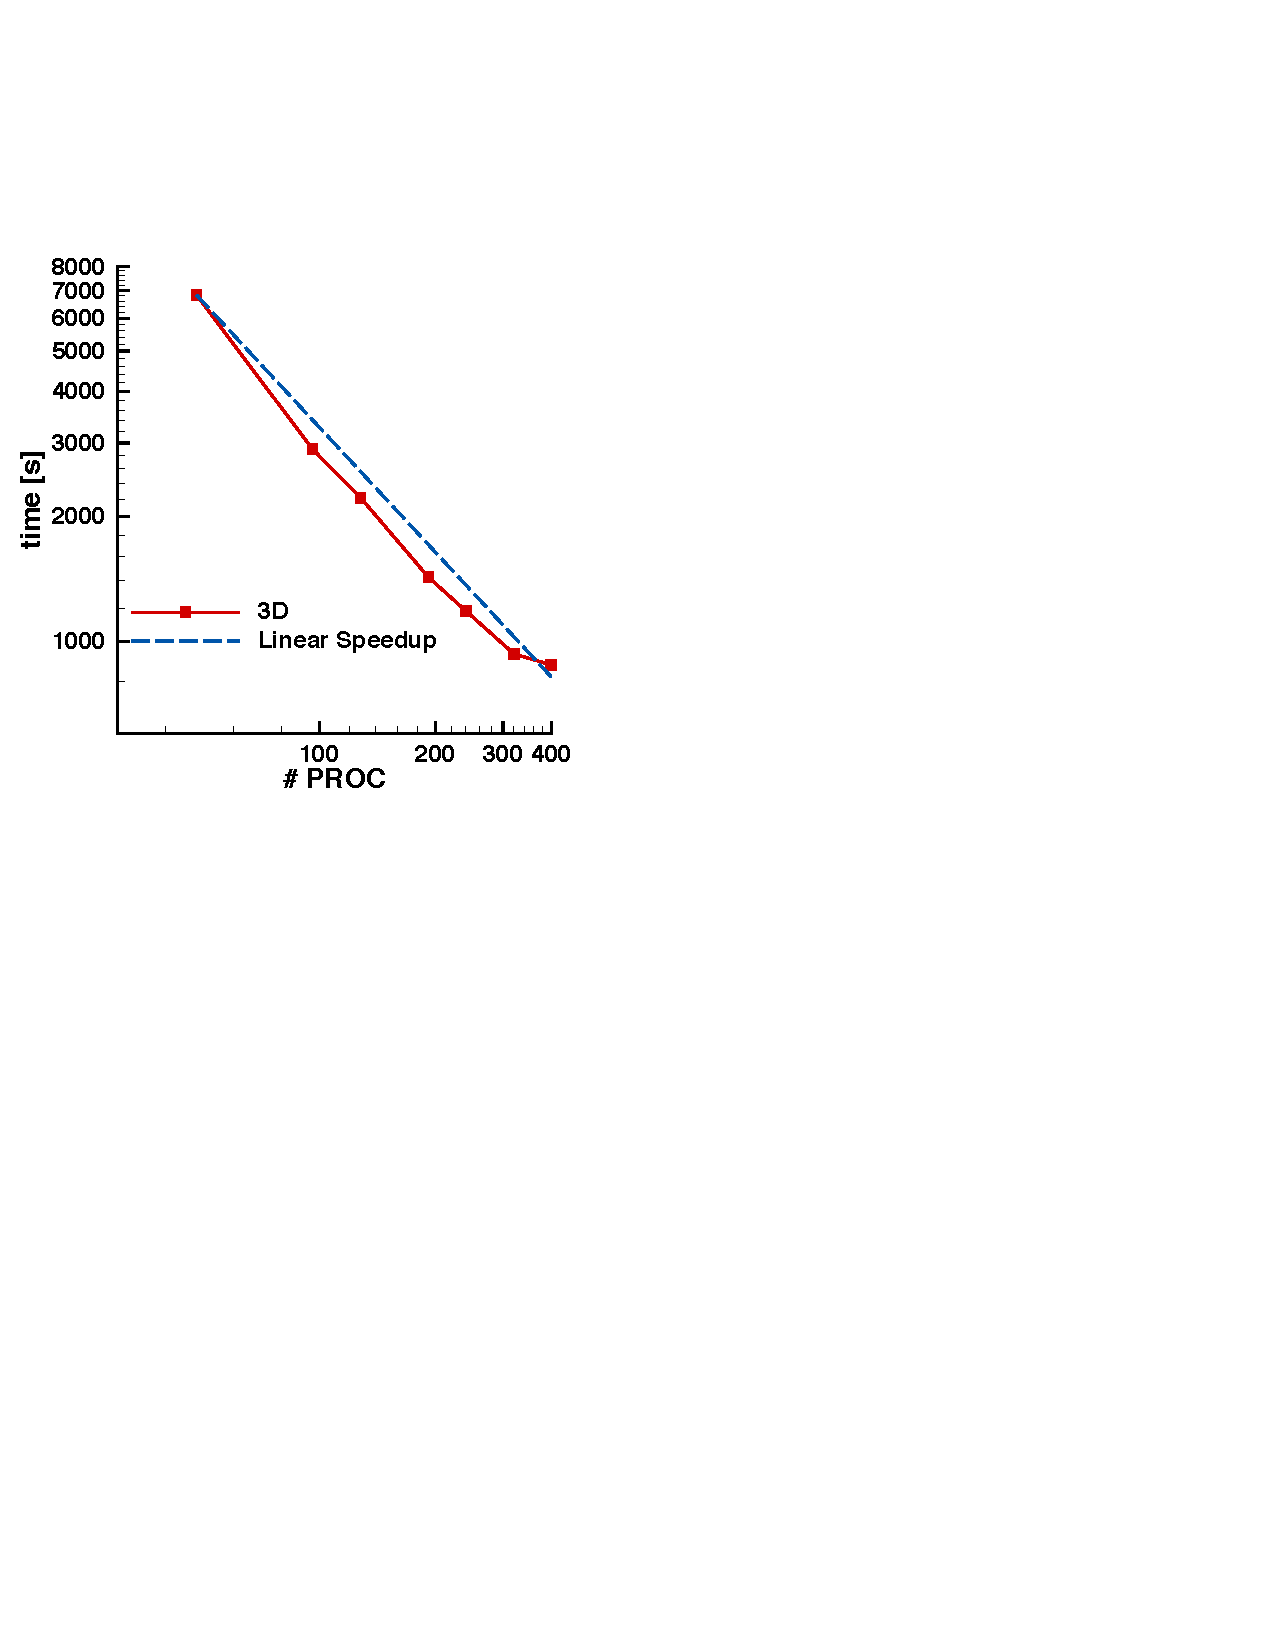
\includegraphics[width=.45\textwidth]{\figpath/Fig_cap_natconv/Scal_ffddm_2level}}
 {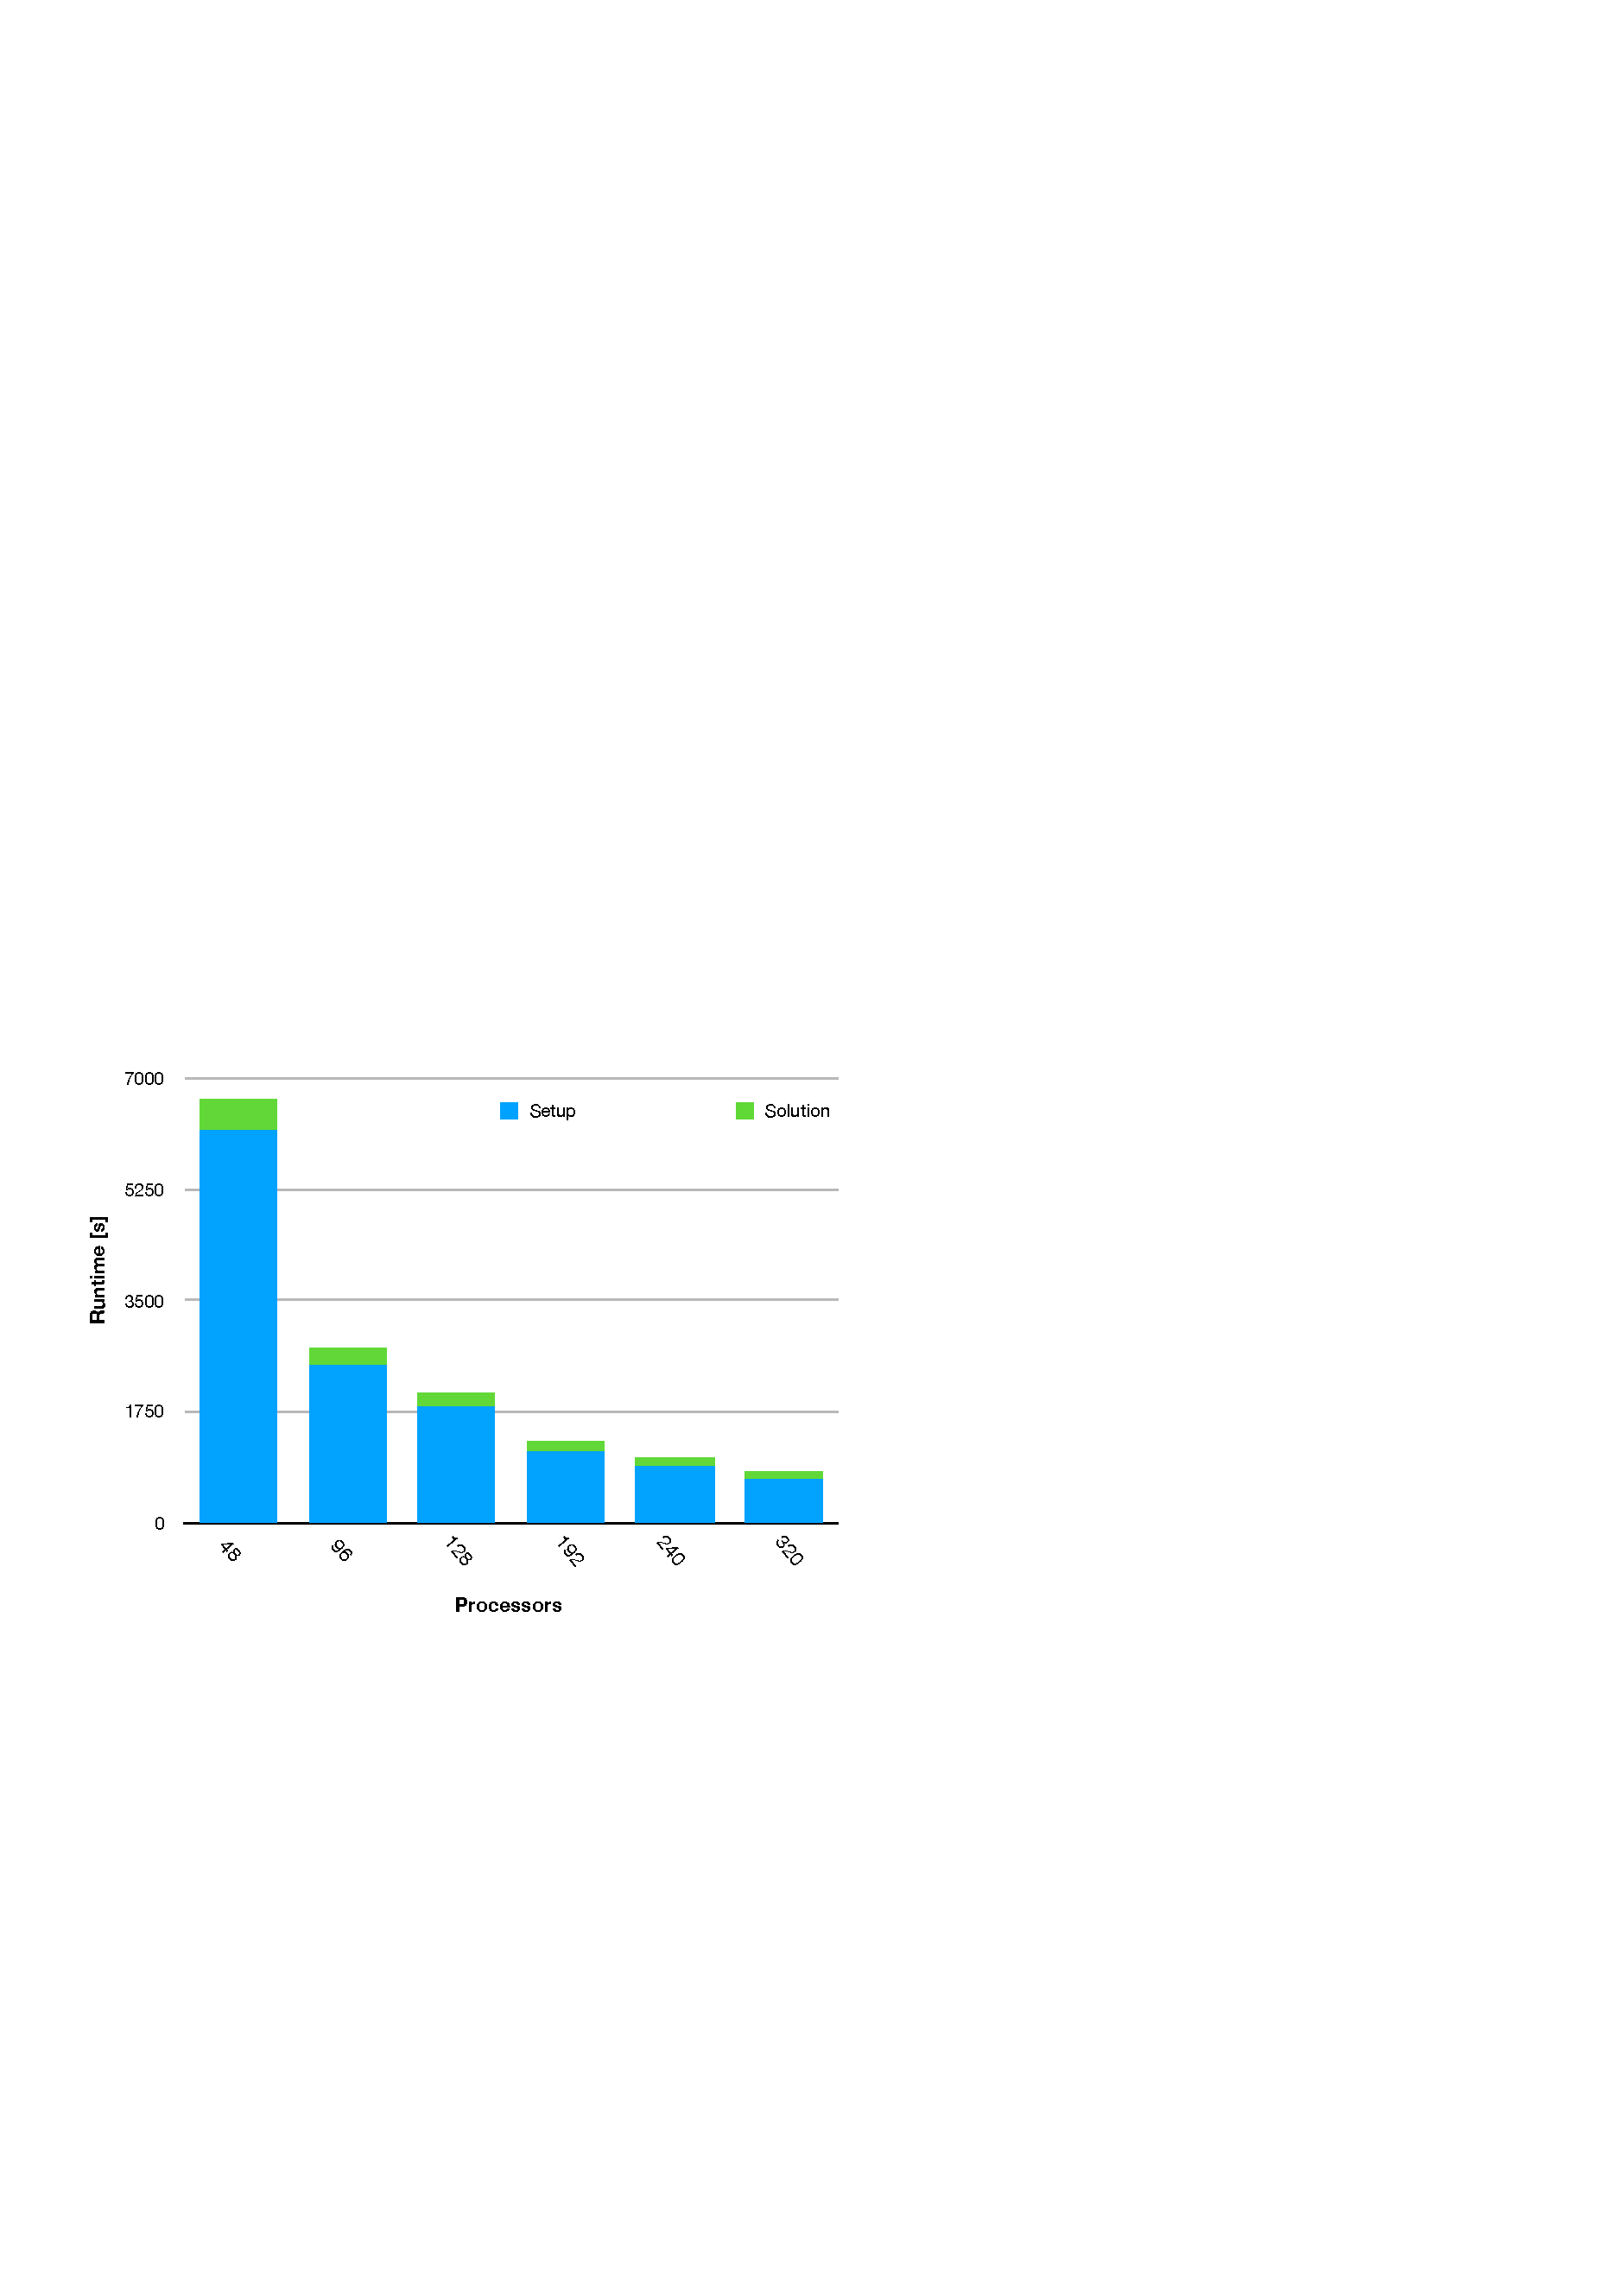
\includegraphics[width=.5\textwidth]{\figpath/Fig_cap_2/scal_ffddm_P2}}
\end{center}
\end{minipage}
\caption{Strong scalability of the ORAS preconditioner: $7.2$ millions of d.o.f and subdomains ranging from $48$ to $400$.}
\label{fig-scalability} 
\end{figure}

\begin{table}[!h]
	\begin{center}
		\begin{tabular}{cccc}
			 $\mathcal{N}$ & Factorization (s)  & GMRES (s)  & Total Step (s) \\ \hline \hline
			 48 & 6186.33  & 473.66  &  6659.99 \\
			 96 & 2468.68  & 283.099 &  2751.779 \\
			 128 & 1814.26 &  237.853 &   2052.113\\
			 192 & 1111.5  &   169.174 &  1280.674 \\
			 240 & 889.422  & 146.539 &  1035.961\\
			 320 & 674.204   &  114.346 & 788.55 \\
			 400 & 614.418  &  107.422 &  721.84\\ \hline
		\end{tabular}
	\end{center}
	\caption {Strong scaling experiment in 3D differentially heated cavity. $7.2$ millions of d.o.f and subdomains ranging from $48$ to $400$. }
	\label{tab-scalability}
\end{table}



\graphicspath{{\figpath/Fig_cap_natconv}}
%%%%%%%%%%%%%%%%%%don't forget if needed %%%%%%%%%%%%%%%%%%%%%
%\section[toc version]{title version%
%              \sectionmark{head version}}
%\sectionmark{head version}
%%%%%%%%%%%%%%%%%%%%%%%%%%%%%%%%%%%%%%%%%%%%%%%%%%%%%%%%%%%%%%
\def\titcourt{Numerical simulation of natural convection flow}
\def\titlong{Numerical simulation of natural convection flow}
%%%%%%%%%%%%%%%%%%%%%%%%%%%%%%%%%%%%%%%%%%%%%%%%%%%%%%%%%%%%%%%%
\chapter[\titlong]{\titlong%
              \chaptermark{\titcourt}}
\chaptermark{\titcourt}
\label{chap-NATCONV}
%%%%%%%%%%%%%%%%%%%%%%%%%%%%%%%%%%%%%%%%%%%%%%%%%%%%%%%%%%%%%%%%
%%%%%%%%%%%%%%%%%%%%%%%%%%%%%%%%%%%%%%%%%%%%%%%%%%%%%%%%%%%%%%%%

We first focus on the capability of our code to deal with natural convection flow in enclosures without phase-change.
The richness of studies on internal natural convection flow indeed allows us to validate the Navier-Stokes-Boussinesq solver in the fluid part.
A large number of benchmark solutions exists in the literature for natural convection induced by temperature difference since it is central in a long list of engineering and geophysical systems
(circulations in building applications, double-wall insulations, solar collectors, etc.).
The influence of the geometric aspect ratio, the inclination, the heating orientation (if we heat from the side of from below), the $\Ray$ number have been widely studied.
It is indeed well-known that the heat transfer is completely different from tall enclosure or shallow enclosure limits. 
In one case, the heat transfer is dominated by conductive transfer (such as double-wall insulations) and in the second case the heat transfer is dominated by the presence of vertical layer.
In this chapter, we are interested in natural convection of fluid in a square cavity differentially heated from the vertical walls.
Along the heated wall, the fluid temperature rises and its density decreases. 
Due to the density decrease, the fluid rises up to the point where it reaches the cold wall, where the reverse process occurs. 
This two simultaneous opposing effects create a recirculation cell. In the center of the cell, a stationary zone can be observed.

We solve the system of eqs. (\ref{eq-qmvt}) - (\ref{eq-energ}) without the penalty term $A(\theta) \vec u$ in the momentum equation and the source term $\partial (CS)/\partial t$ in the energy equation.
Linear and non-linear expressions of the buoyancy force $f_B(T)$ in the Boussinesq approximation (\ref{eq-energie-enth-model}) are investigated, by simulating the natural convection of air and the natural convection of water.
Natural convection of water exhibits actually a non-linear variation of the density with a maximum value around $T=4^o C$ while linear variation is generally assumed for the natural convection of air in the Boussinesq approximation.

We consider a cavity of height $H$ and the physical property of air and water are listed in tab. (\ref{tab-param-phys-air}):
\begin{table}[ht!]
   \begin{center}
      \begin{tabular}{*{8}{cl}}
         
        & $\rho$ &$ \mu$ & $c_p $ & $k$ & $\alpha $ & $\beta$ \\
        & kg/m$^3$& kg/(m s) & J/(kg K) & W/(m K) & m$^2$/s & 1/K \\
         \hline
        Air & 1.177 & 1.85 $\cdot 10^{-5}$  & 1006 & $0.0262$ & $2.22 \cdot 10^{-5}$ & $3.4 \cdot 10^{-3}$ \\
        Water & 999.84 & 1.003 $\cdot 10^{-3}$  & 4182 & $0.6$ & $1.33 \cdot 10^{-7}$ & $6.91 \cdot 10^{-5}$
      \end{tabular}
   \end{center}
   \caption{Physical parameters of air and water at $T = 300K$, used in our simulations. For air these parameters lead to dimensionless $\Pr = 0.71$ and $\Pr = 6.99$ for water.}
   \label{tab-param-phys-air}
\end{table}

Isothermal boundary conditions are applied to the vertical walls and adiabatic boundary condition to the upper and lower walls.
Quantitative and qualitative validations are carried out for both natural convection of air and water in two and three-dimensional configurations as follows: \newline{}
{\bf(i)} Natural convection of air in a two dimensional square cavity: velocity profile along symmetry lines, the maximum value of $u_{max}$ at mid-domain($x=0.5$) and location $Y$ of this maximum  are compared with the spectral-accurate simulations by \cite{LeQuere91} in sec. \ref{sub-diff-heated}, \newline{}
{\bf(ii)} Natural convection of air in a 2D square cavity with inner heated square obstacle: transversal velocity profile along the  horizontal symmetry lines is compared with numerical results of \cite{Raluca2013} 
in sec. \ref{sub-2D-OBSTACLE}, \newline{}
{\bf(iii)} Natural convection of water if a 2D square cavity: Temperature profile along the horizontal symmetry line is compared with the numerical results of \cite{Kowalewski-2003} in sec. \ref{sec: natconv-water}.
{\bf(iv)} Natural convection of air in a cube: the temperature field is qualitatively compared with numerical results of \cite{Wakashima-2004} and a comparison between ffddm and the sequential algorithm is given in 
sec. \ref{sec: natconv-air-3D}, \newline{}
{\bf(v)} Natural convection of air in a cube with a cubic heated obstacle is presented in sec. \ref{sub-OBSTACLE-3D}.

\section{Natural convection of air in a two dimensional square cavity}\label{sec: natconv-air-2D}
We start by testing the Newton algorithm (\ref{eq-newton-C1}) by investigating simulations with linear expression of $f_B(\theta)$ as presented in eq. (\ref{eq-RePr}).
The classical problem of the thermally driven square cavity with adiabatic top and bottom walls is of interest.
A square cavity of height $H = 0.1$m, initially filled with motionless air with a linear distribution of the temperature is considered. 
The dimensionless parameters describing the investigated configuration are based on the fluid properties presented in tab. (\ref{tab-param-phys-air}), mainly $\Pr = 0.71$.
Three $\Ray$ numbers are computed $Ra = 10^4, 10^5, 10^6$, and
the characteristic scales of the problem defined in eq. \ref{eq-adim} are:
\begin{equation} \label{eq-scale-air}
	L_{ref} = H, \quad T_{ref} = \frac{T_h + T_c}{2},
\end{equation}
and
\begin{equation}
   V_{ref} = \frac{\nu_l}{H} \sqrt{\frac{Ra}{Pr}} 
   \quad \Longrightarrow \quad t_{ref} = \frac{\nu_l}{H^2} \sqrt{\frac{Pr}{Ra}} 
   \quad \Longrightarrow \quad \Rey = \sqrt{\frac{Ra}{Pr}}.
\end{equation} 
The thermal boundary conditions corresponding to eq. (\ref{eq-scale-air}) are $\theta_h = 0.5$ on the left wall and $\theta_c = -0.5$ on the right wall. 
No-slip boundary condition is applied for the velocity.

It has been shown by \cite{LeQuere91} that the solution of the 2-D Boussinesq equation in this configuration becomes unsteady at $Ra = 10^{8.5}$.
Therefore, steady state can be achieved for the chosen Rayleigh numbers.

The unsteady and steady Navier-Stokes-Boussinesq equations are simulated.
The unsteady case is computed until the steady state with a single convection cell is reached, with a numerical tolerance of $10^{-9}$.
Besides, the steady case is performed using Rayleigh number continuation:
a smaller value of the Rayleigh number is set initially, and is then increased smoothly until reaching the correct value.
At each stage, the computation starts from the solutions obtained from the previous Rayleigh number simulation.

Two cases are carried out: {\it i)} a differentially heated square cavity and {\it ii)} a differentially heated cavity with inner heated obstacle.
For each of them, the horizontal and the vertical velocity profiles $u(y)$ and $v(x)$ at mid-domain ($y=0.5$ and $x=0.5$ respectively) are plotted and compared with numerical result by \cite{LeQuere91} and \cite{Raluca2013}. 
Moreover, for {\it i)} the maximum value $u_{max}$ and its location $Y$ are accurately compared with the solutions obtained by spectral accurate simulations by \cite{LeQuere91}.

\subsection{Differentially heated square cavity} \label{sub-diff-heated}
All computations in this section are performed with a fixed triangular mesh, generated by the Delaunay algorithm starting with M = 80 points on each side of the square.
Fig. \ref{fig-T1-prof} illustrates a comparison of the horizontal (Fig. \ref{fig-T1-prof}a) and the vertical (Fig. \ref{fig-T1-prof}b)  profiles of the velocity with data extracted from  \cite{LeQuere91}.
Results from \cite{LeQuere91} are represented by solid lines and the current simulation by symbols.
A very good agreement can  be noticed for each of the three Rayleigh numbers.

\begin{figure}
	\begin{center}
		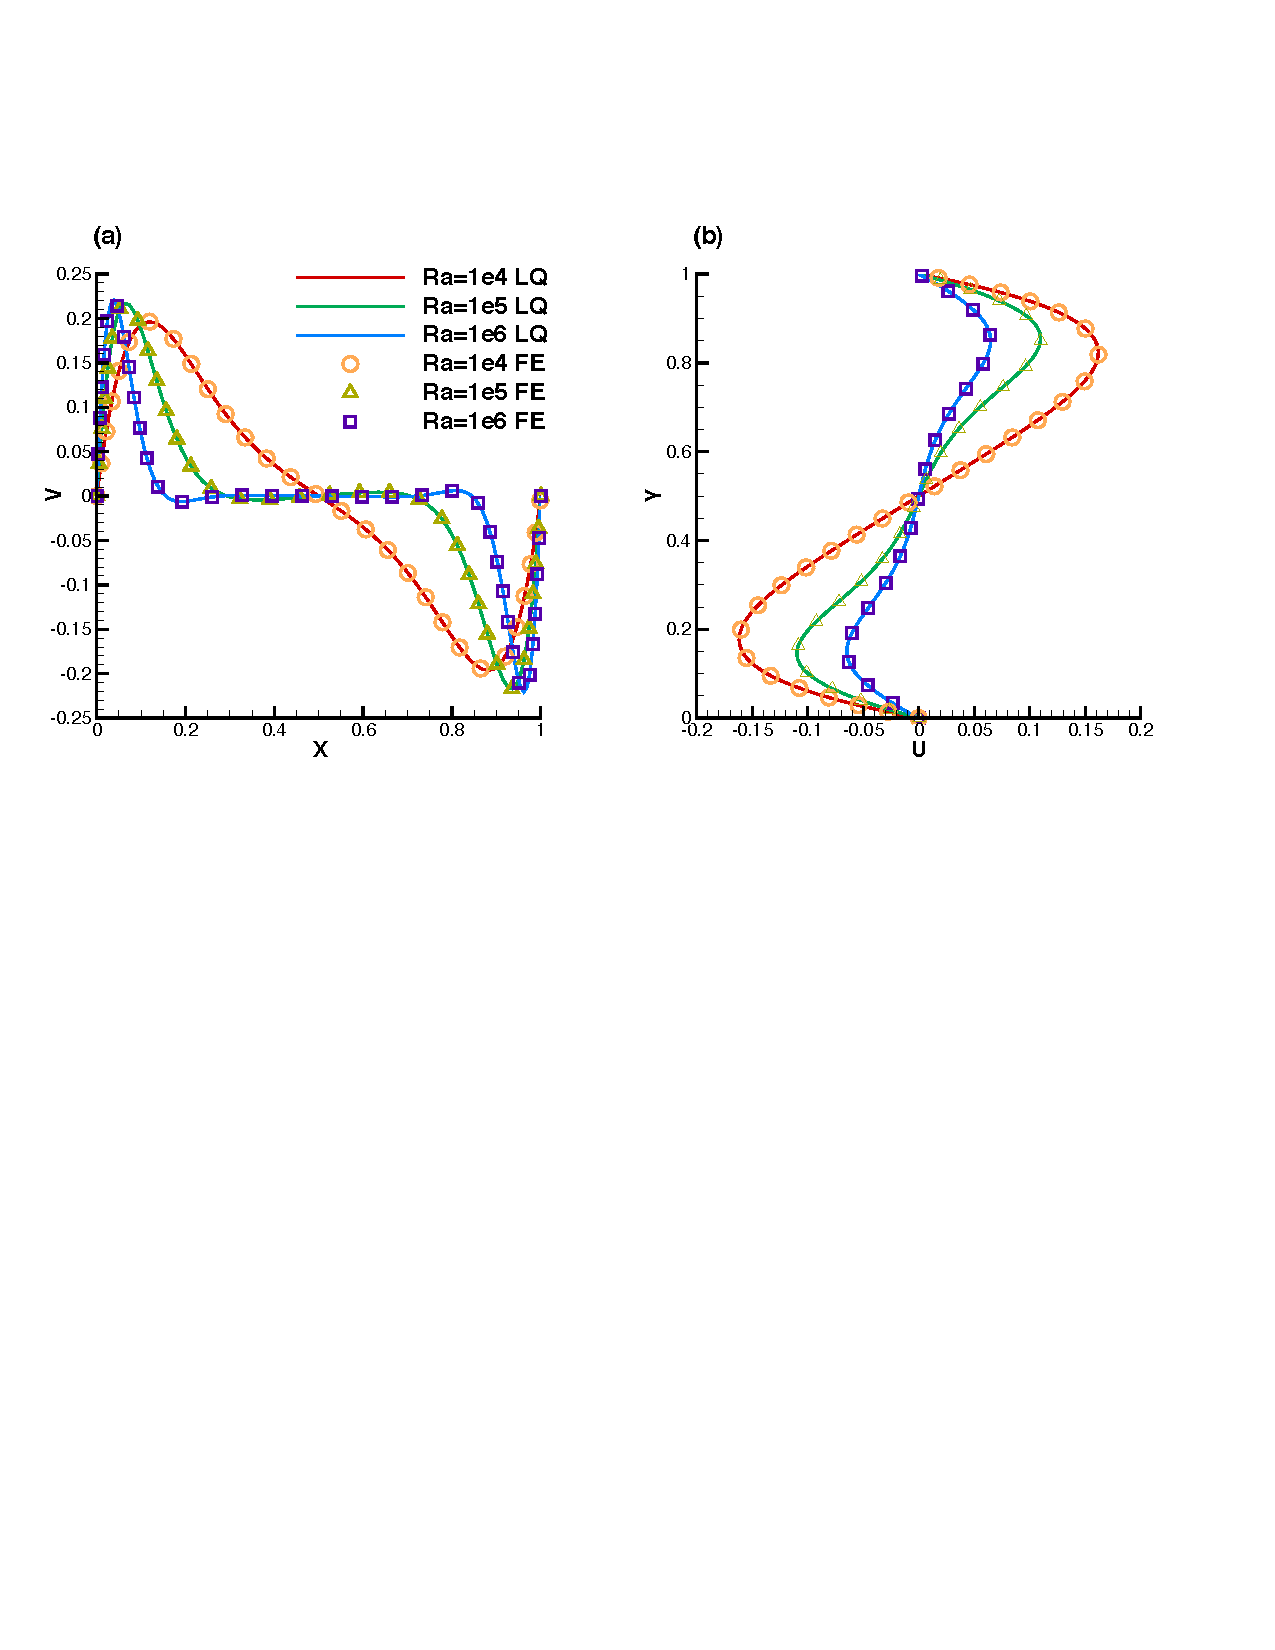
\includegraphics[width=0.98\textwidth]{\figpath/Fig_cap_natconv/Validation_Uprofile_LQ} 
	\end{center}
	\caption{Natural convection of air in a differentially heated cavity for $Ra$ ranging from $10^4$ to $10^6$ and $\Pr = 0.71$. (a) Transversal velocity profile along the  horizontal symmetry lines. (b) Longitudinal velocity profile along the vertical symmetry lines. Numerical results obtained using the present Newton method (symbols) with a mesh resolution of $M=80$; comparison with the spectral-accurate simulations by \cite{LeQuere91} (solid lines).}
	\label{fig-T1-prof}
\end{figure}

The influence of the imposed temperature difference $\delta T$ on the boundary layers are well illustrated in Fig.  (\ref{fig-T1-prof}).
Eq. (\ref{eq-corr-Low-Pr}) indicates a decreasing thickness of the boundary layer for an increasing value of $\Ray$. 
For $\Ray = 10^6$ a viscous boundary layer with a dimensionless thickness of order of $\delta_\nu \sim 0.02$ should be present close to the vertical walls.
Accordingly, the mesh resolution should allow to capture these structures.
A mesh convergence analysis shows a reasonable relative error (lower than $3\%$) from a $80 \times 80$ grid resolution.
Also, from $\Ray = 10^5$ the fluid in the core of the cavity is relatively stagnant and thermally stratified.
This indicates that for $\Ray < 10^5$, the heat transfer is dominated by the bulk heat transfer, while for $\Ray \geq 10^5$ the heat transfer is boundary layer heat transfer.

Tab. (\ref{tab-valid-natconv}) offers a quantitative assessment of the accuracy of the present Newton method. 
The values of $u_{max}$  and its location $Y$ are compared to reference values from \cite{LeQuere91}. 
The Newton method gives results very identical to reference values, with a relative difference less than $0.01 \%$ for the steady and the unsteady codes. 
The characteristics-Galerkin method is less accurate, but still offers reasonable agreement with reference values, within 2$\%$ relative error. 
We also recall that the characteristics method needs a very small time step for refined meshes ($\delta t = 8\cdot 10^{-5}$ for $M=80$), while the Newton method allows larger time steps ($\delta t = 1$ for $M=80$). % and consequently, converges faster to a steady state.
%It is worth noting, that the steady and the unsteady codes provide quasi-identical results.
\begin{table}%[!h]
	\begin{center}
		\begin{tabular}{|l|c|l|l|}
			\hline
			\multicolumn{2}{|l|}{Run} & $u_{max}$ at x=$0.5$ (error) & $Y$ (error) \\
			\hline
			Reference values & spectral & 0.0648344           & 0.850 \\ \hline
			Char-Galerkin       &$M=80$ & 0.0662229 (2.14 $\%$) & 0.856160 ( 0.72 $\%$) \\ \hline
			\cite{dan-2014-JCP}              &$M=80$ & 0.0650082 (0.26 $\%$) & 0.849906 ( 0.01 $\%$) \\ \hline
			Newton (Steady)        &$M=80$ & 0.0648297 (0.007 $\%$) & 0.850394( 0.05 $\%$) \\ \hline
			Newton (Unsteady)        &$M=80$ & 0.0648296 (0.007 $\%$) & 0.850532 ( 0.06 $\%$) \\ \hline
		\end{tabular}
	\end{center}
	\caption {Natural convection of air in a differentially heated cavity for $Ra = 10^6$ and $\Pr = 0.71$. Maximum value $u_{max}$ of the horizontal velocity profile at mid-domain ($x=0.5$) and location $Y$ of this maximum. Comparison to reference values by \cite{LeQuere91}.}
	\label{tab-valid-natconv}
\end{table}

\subsection{Differentially heated cavity with inner heated square} \label{sub-2D-OBSTACLE}

\begin{figure}
	\begin{center}
		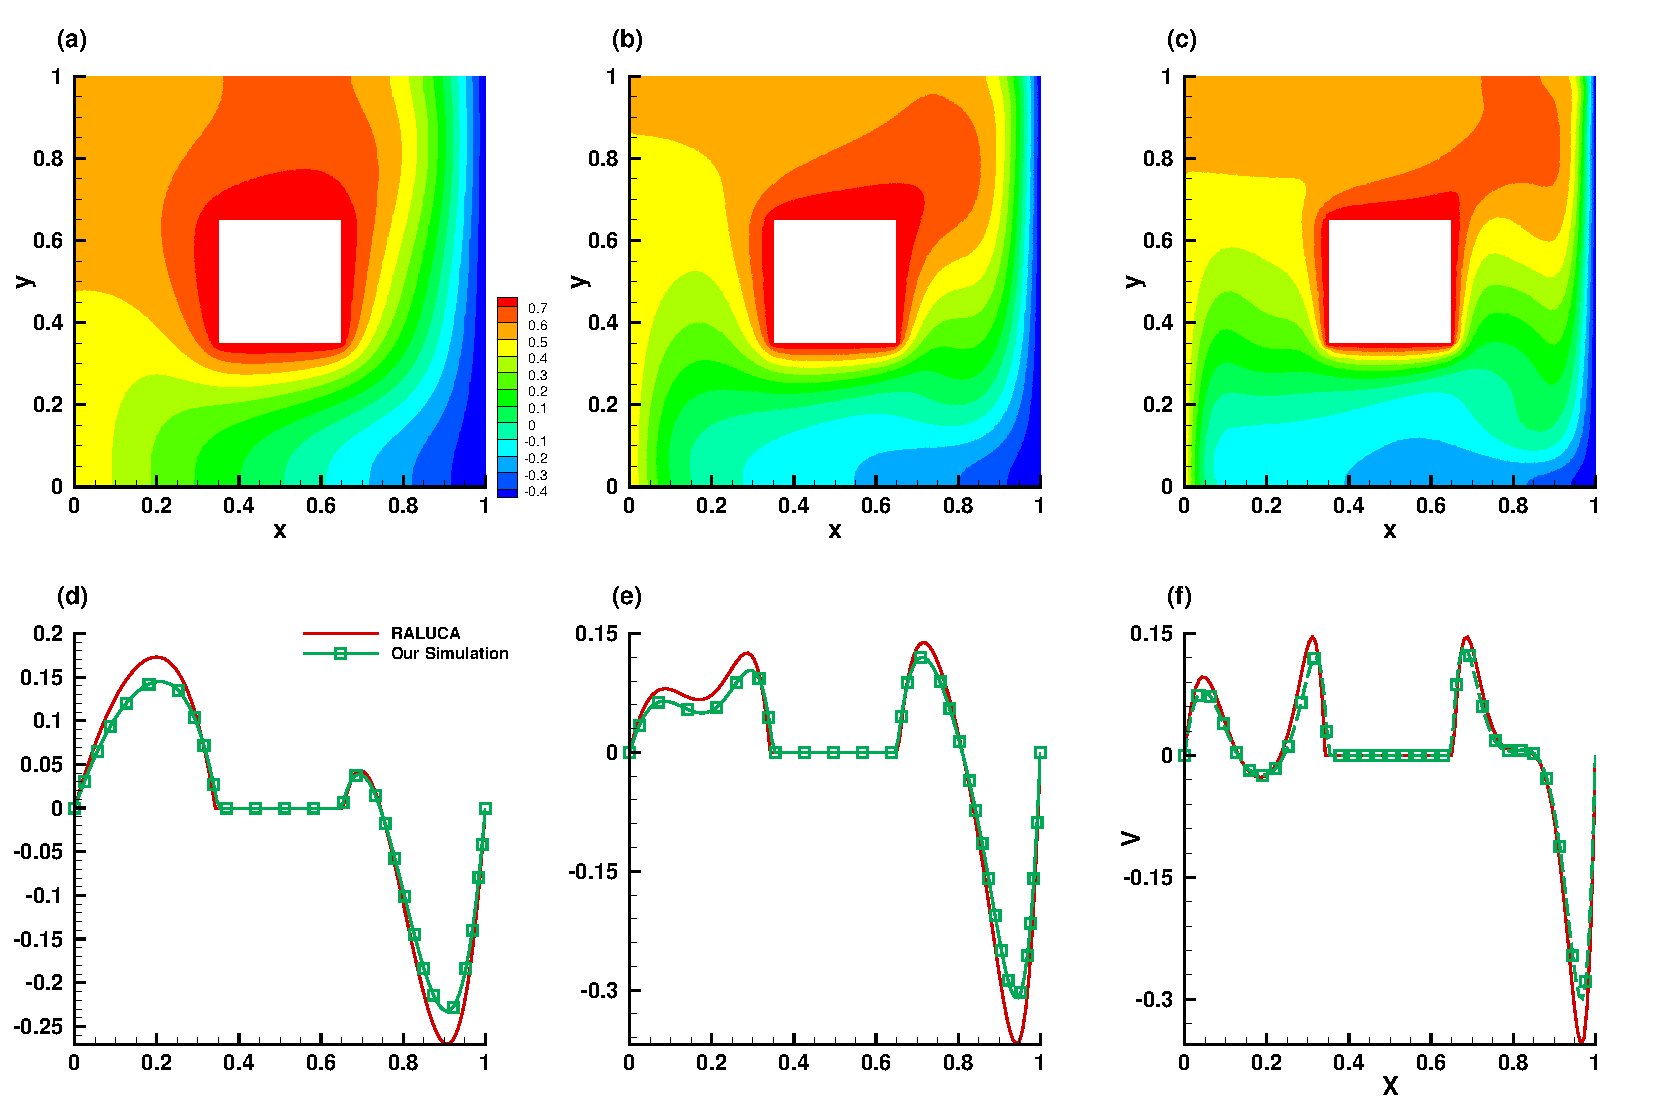
\includegraphics[width=\textwidth]{\figpath/Fig_cap_natconv/STA_validation_obstacle_2} 
	\end{center}
	\caption{Natural convection of air in a differentially heated cavity with inner heated square for $Ra = 10^6$. Temperature field (a) and transversal velocity profile along the  horizontal symmetry lines (b). Results obtained using the present Newton method (red solid line), with mesh resolution $M=80$; comparison with the finite difference code of \cite{Raluca2013}.}
	\label{fig-obst-2D}
\end{figure}

Thermally driven cavity including heated square obstacle is computed in this section.
We consider the same configuration presented in sec. \ref{sub-diff-heated} and a square involving isothermal boundary condition is added between the initial set up.
This kind of basic configuration could be representative of telecommunication outdoor cabinet applications, in which the use of passive cooling solutions have begun to be more and more investigated.
Indeed, inside an outdoor cabinet, electronic equipments generate heat when active and the study of the flow structures within the enclosure have attracted some considerations at the example of the experimental and numerical study of \cite{Raluca2013}.
Simplified model of cavity with rectangular heated obstacles have been investigated by \cite{Raluca2013} and will be reproduced in this section to test the robustness of our numerical algorithm.

A linear distribution of the temperature is imposed initially in the motionless air inside the cavity.
The obstacle is maintained at a dimensionless hot temperature $\theta_h = 0.8$ with a no-slip boundary condition for the velocity.
The solutions for $Ra = 10^4$, $Ra = 10^5$, $Ra = 10^6$ and $Pr = 0.71$ are compared with the result obtained by \cite{Raluca2013} who used an immersed boundary method with a FD code using high order schemes for time and spatial discretization.

The temperature distribution in the cavity when the steady-state is reached, for each of the three $\Ray$ number computed, are shown in panels (a) to (c) of Figs. \ref{fig-obst-2D}.
The temperature gradient gives rise to a clockwise circulation and when $\Ray$ is increased, vertical thermal boundary layers form distinctly along the differentially heated sidewalls and the obstacle.
Consequently, 
higher is the Rayleigh number the more the hot temperature in the center of the domain is advected by the natural convection flow into the cold part of the cavity. 
Worth noting is the fact that at $\Ray = 10^6$ in panels (c) and (d), a stagnant fluid with a stratified temperature forms in a small portion of the fluid between the cold wall and the obstacle.

A more accurate validation is given in panels (d) to (f) of Fig. (\ref{fig-obst-2D}).
The transversal velocity profiles along the x-axis are plotted and compared with the numerical data of \cite{Raluca2013} for each of the three $\Ray$ number investigated. 
A good agreement can be observed with a relatively small differences between the extremum of the velocity while the trends of the velocity profile match well.

We have demonstrated in this part that the proposed Newton method offers an efficient way to solve the Navier-Stokes-Boussinesq system of equations for natural convection of air evolving a linear expression of $f_B(\theta)$.
A further difficulty will be introduced in the next section when a non-linear expression of the body force is defined since natural convection of water is of interest.
%We can conclude from this section that the proposed Newton method offers an efficient way to solve the Navier-Stokes-Boussinesq system of equations for natural convection. After this validation, we test in the following section the capability of the method to deal with phase-change, introducing nonlinearity in the momentum and the energy equations.

\section{Natural convection of water in a two dimensional square cavity}\label{sec: natconv-water}
We investigate in this section the natural convection of water in a differentially heated cavity. 
A further difficulty is taken into account compared to the previous validation by introducing non-linear variation of the density in the buoyancy force.
Pure water involve actually non-linear density variation for $T< \celsm{10.2}$ with a maximum at $T_m= \celsm{4.0293}$. 
We use below the following density-temperature relationship  proposed in \cite{Gebhart1977}:
\begin{equation}
\rho(T)=\rho_m \left(1 - w \left|T - T_m\right|^q\right),
\end{equation}
with $\rho_m=999.972$ [kg/m$^3$], $w=9.2793\cdot 10^{-6}$ [($^\circ C)^{-q}$], and $q=1.894816$.
The bouyancy term $f_B = g(\rho_\vref-\rho)/\rho_\vref$ appearing in eq. (\ref{eq-momentum-conserv})  becomes after scaling:
\begin{equation}
f_B(\theta) = \frac{\Ray}{\Prd \, \Rey^2} \frac{1}{\beta \delta T}\, \frac{\rho(\theta_f)-\rho(\theta)}{\rho(\theta_f)},
\label{eq-fBnonlin}
\end{equation}
where $\beta=(1/\rho_m) \left(d\rho/dT\right)$ is the thermal expansion coefficient with the value \cite{Scanlon2004} $\beta=6.91 \cdot 10^{-5}$ [(K)$^{-1}$].

We simulate a differentially heated cavity of height $H = 0.38 m$ filled with liquid pure distilled water.
This problem was investigated experimentally and numerically in \cite{Giangi-2000,Kowalewski-1999,Kowalewski-2003}.
The height $H$ of the cavity is considered as a length scale of the problem $L_{ref} = H$. 
We choose $T_{ref} = T_h - T_c$ in order to compare our simulation with the numerical results of \cite{Kowalewski-2003},
and define the following scaling:
\begin{equation}
   V_{ref} = \frac{\nu_l}{H} 
   \quad \Longrightarrow \quad t_{ref} = \frac{\nu_l}{H^2}
   \quad \Longrightarrow \quad \Rey = 1.
\end{equation} 
The non-dimensional parameters describing the problem result from the physical properties of water in Tab. \ref{tab-param-phys-air}: $\Ray=2.518084\cdot 10^{6}$ and $\Pr=6.99$. %  (see also \cite{Kowalewski-2003} for physical details). % and $\Ste = 6.99$.

The initial temperature is linearly distributed with a hot temperature $T_h =\celsm{10}$ at the left wall and a cold temperature $T_c=T_f=\celsm{0}$ at the right wall, corresponding to dimensionless thermal boundary condition $\theta_h = 1$ and 
$\theta_c = 0$. The top and the bottom of the cavity are adiabatic and no-slip boundary condition $\vec u = 0$ is used for the velocity.

The Temperature field of the steady state is presented in Figure \ref{fig-T1w-isoT}a and a more accurate comparison of the temperature profile along the horizontal symmetry line is given in Figure \ref{fig-T1w-isoT}b. 
The isoline $\theta = \theta_m$, corresponding to the line of maximum density is presented in Figure \ref{fig-T1w-isoT}a by dashed line.
Indeed, due to the anomalous thermal variation of water density, two recirculating zones are formed in the flow: a lower (abnormal) recirculation  in the vicinity of the cold wall where $\theta<\theta_m$ and an upper (normal) one where the density decreases with temperature ($\theta>\theta_m$).

The temperature profile $\theta(x)$ along the horizontal symmetry line of the cavity is in good agreement with the numerical results   of \cite{Kowalewski-2003} obtained with FV and FD codes (FLUENT and FRECONV3V), commonly used in the heat transfer community. Differences are visible in the vicinity of the maximum density line, region where our mesh is well refined to capture the separation line between the two recirculation zones. It should be noted that the FLUENT simulations in \cite{Kowalewski-2003} are performed with a fixed uniform grid with $380\times380$ nodes, while our adapted grid has only 8751 vertices (17257 triangles).

\begin{figure}
	\begin{center}
		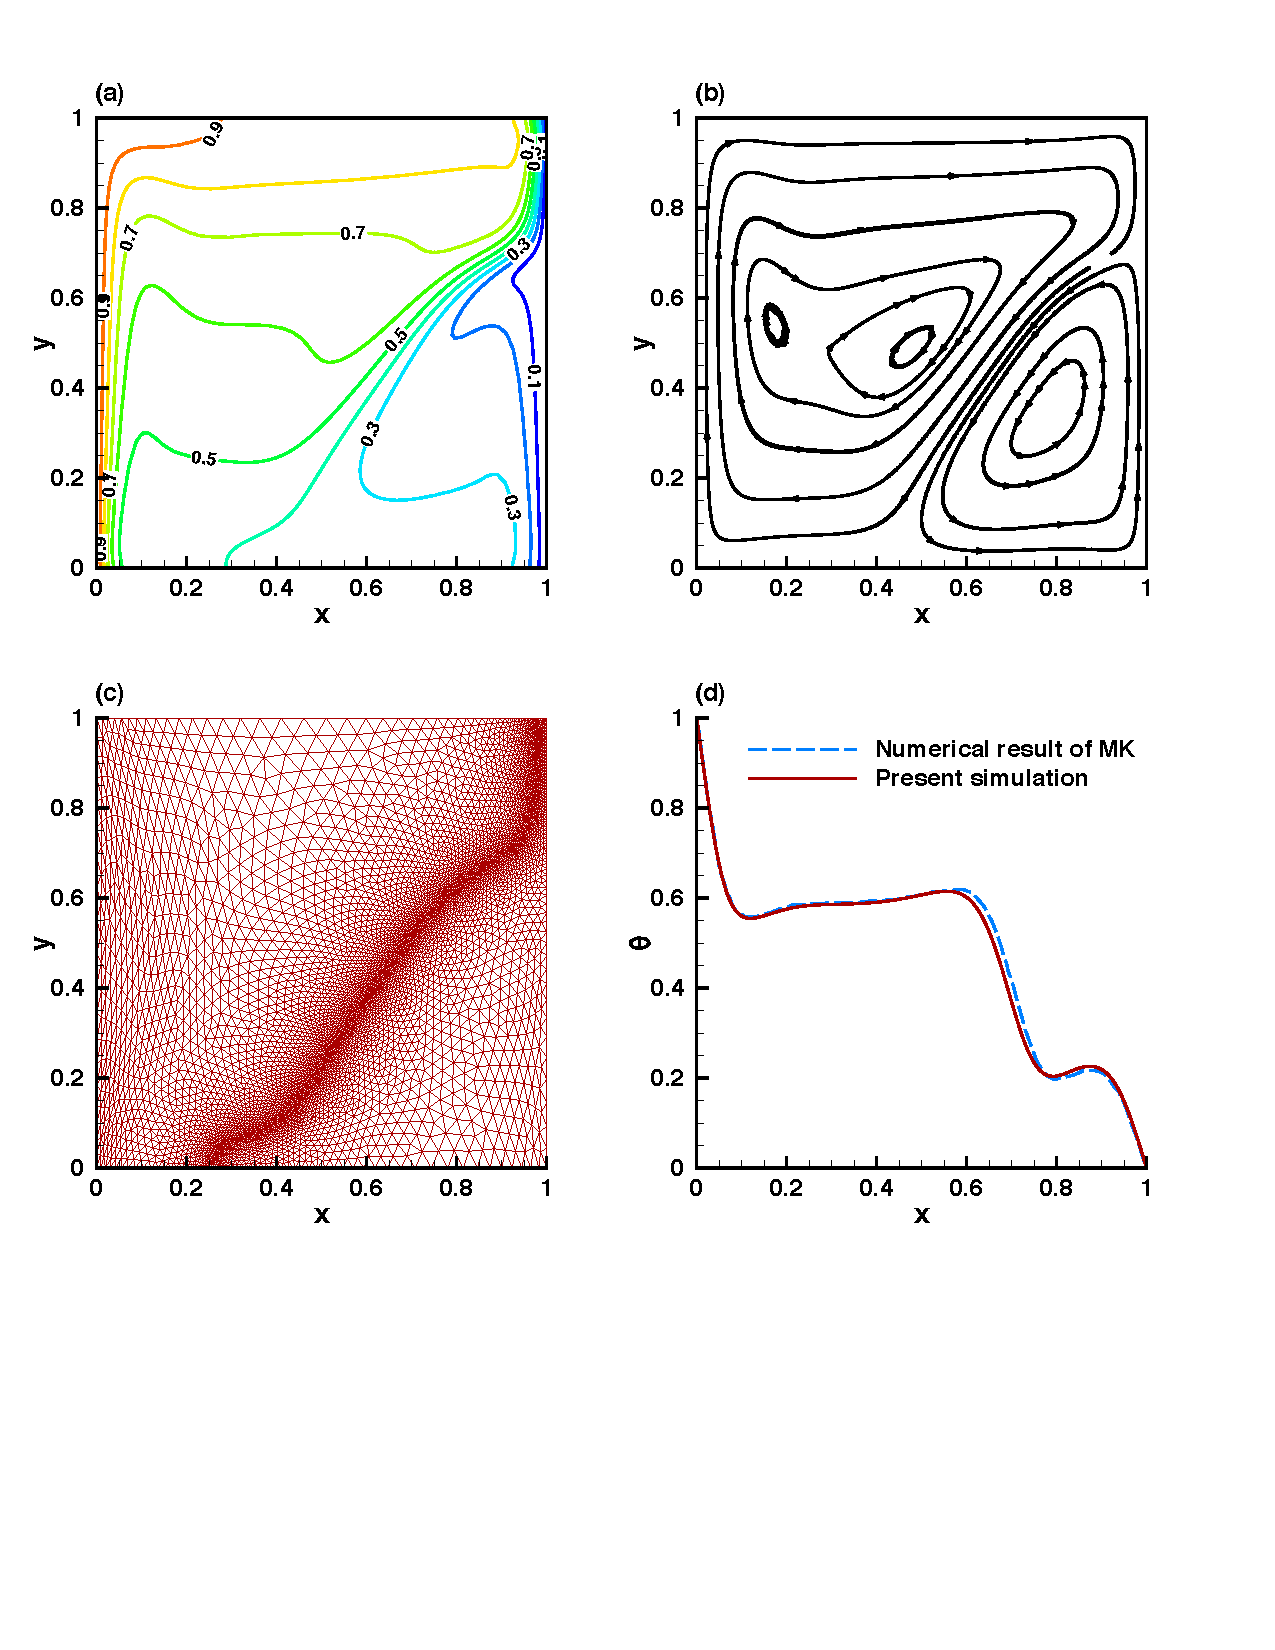
\includegraphics[width=0.98\textwidth]{\figpath/Fig_cap_natconv/WATER_convec_valid}
	\end{center}
	\caption{Natural convection of water in a differentially heated cavity with non-dimensional parameters: $\Ray=2.518084\cdot 10^{6}$ and $\Pr=6.99$. (a) iso-line of the temperature at the steady state. (b) Streamline of the steady flow. (c) Illustration of the mesh adaptivity: The mesh is refined along the dimensionless temperature iso-line $\theta = 0.4$ due to the density variation. (d) Temperature profile along the horizontal symmetry line. Comparison with the numerical results of \cite{Kowalewski-2003}.}
	\label{fig-T1w-isoT} % label should be placed after the caption
\end{figure}

\section{Natural convection of air in a three dimensional cavity using FFDDM}\label{sec: natconv-air-3D}

\subsection{Natural convection in a differentially heated cube cavity}
We present in this section some 3D simulations using ffddm.

%A schematic model of the problem is displayed in figure \ref{fig-3Dmesh} a).
The Prandtl number is $0.71$ and three Rayleigh numbers are considered:  $\Ray=10^4$, $\Ray=10^5$, $\Ray=10^6$. The walls are rigid and impermeable. The vertical walls at $x=0$ and $x=1$ are isothermal and have different temperatures $T_h=0.5$ and $T_c=-0.5$ respectively. The remaining walls are considered adiabatic. % Figure \ref{fig-3Dmesh} b) shows the present three dimensional grid.
%\begin{figure}%[!htbp]
%\begin{minipage}{0.45\linewidth}
%\begin{center}
% {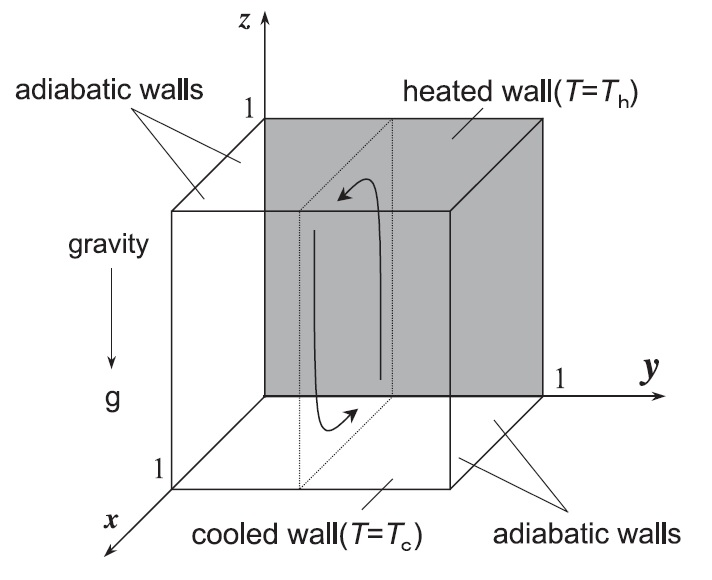
\includegraphics[width=1.\textwidth]{\figpath/Fig_cap_natconv/3D_scema.jpg}}\\
% a)
%\end{center}
%\end{minipage}\hfill
%\begin{minipage}{0.45\linewidth}
%\begin{center}
% {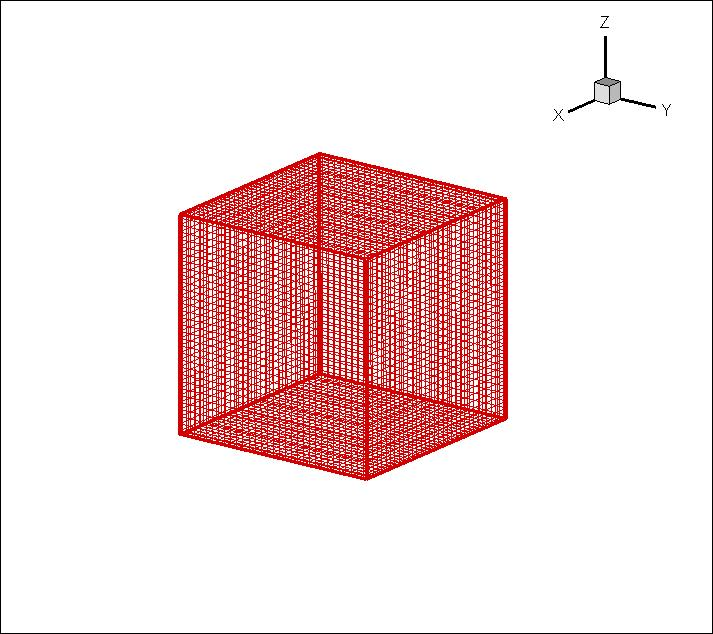
\includegraphics[width=1.\textwidth]{\figpath/Fig_cap_natconv/mesh3D.jpg}}\\
% b)
%\end{center}
%\end{minipage}
%\caption{(a) Schematic model for the natural convection in a cubic cavity; (b) present 3D uniform mesh.}
%\label{fig-3Dmesh}
%\end{figure}
 
Our result were obtained for uniform grids of $  40 \times 40 \times 40$ and is compared with \cite{Wakashima-2004} who used a forth order finite difference method, with a vorticity-stream function formulation with different uniform meshes of  $120 \times 120 \times 120 \times 10$ grid nodes. 
This result obtained with sequential algorithm is also used to validate the 3D simulations using ffddm.

Fig. \ref{fig-3DT} shows the temperature field for each of the three Rayleigh numbers $\Ray = 10^4$, $\Ray = 10^5$, $\Ray = 10^6$, at the mid section (y=0.5).
On the left we display the numerical results of \cite{Wakashima-2004} and on the right ou results.
The comparison with the benchmark solution exhibits a fairly good agreement.

The parallel algorithm used with ffddm is compared with the sequential algorithm.
$\mathcal{L}_2$-norm and $\mathcal{L}_\infty$-norm of the velocity and the temperature are computed and reported in Tab. \ref{tab-T1} for Rayleigh number varying from $10^4$ to $10^6$.
The difference between both algorithm is of order of $10^{-6}$.
Moreover, we do not observe a large variation of the error when the number of subdomains is increased.
The number of subdomain vary from $28$ to $70$ for $1.8$ millions of unknown.

\begin{table}[!h]
	\begin{center}
		\begin{tabular}{|*{6}{c|}}
			\hline
			 Ra & nb proc                     & $||u||_{2}$                        & $||u||_{\infty}$                & $||T||_{2}$              & $||T||_{\infty}$\\ \hline \hline
			\multirow{4}{*}{$10^4$} & 28 & $1.12496 \cdot 10^{-6}$ & $3.1 \cdot 10^{-6}$ & $ 3.09966 \cdot 10^{-6} $ & $7 \cdot 10^{-6}$ \\% \hline
			\cline{2-6}
			& 42 & $1.53698 \cdot 10^{-6}$ & $5.1 \cdot 10^{-6}$ & $ 3.23352 \cdot 10^{-6} $ & $8 \cdot 10^{-6}$ \\ \cline{2-6} %\hline 
			& 56 & $1.55576 \cdot 10^{-6}$ & $5.1 \cdot 10^{-6}$ & $ 3.4342 \cdot 10^{-6} $ & $8 \cdot 10^{-6}$  \\ \cline{2-6} %\hline
			& 70 & $1.25622 \cdot 10^{-6}$ & $3.6 \cdot 10^{-6}$ & $ 3.56048 \cdot 10^{-6} $ & $8 \cdot 10^{-6}$ \\ \hline \hline
			\multirow{4}{*}{$10^5$} & 28 & $1.73254 \cdot 10^{-6}$ & $6.1 \cdot 10^{-6}$ & $ 2.40467 \cdot 10^{-6} $ & $7 \cdot 10^{-6}$ \\% \hline
			\cline{2-6}
			& 42 & $2.84973 \cdot 10^{-6}$ & $7.78 \cdot 10^{-6}$ & $ 3.53003 \cdot 10^{-6} $ & $9 \cdot 10^{-6}$ \\ \cline{2-6} %\hline 
			& 56 & $3.00832 \cdot 10^{-6}$ & $7.39 \cdot 10^{-6}$ & $ 4.17769 \cdot 10^{-6} $ & $1.1 \cdot 10^{-5}$  \\ \cline{2-6} %\hline
			& 70 & $3.68118 \cdot 10^{-6}$ & $9 \cdot 10^{-6}$ & $ 4.70846 \cdot 10^{-6} $ & $1.2 \cdot 10^{-5}$ \\ \hline \hline
			\multirow{4}{*}{$10^6$} & 28 & $6.61804 \cdot 10^{-6}$ & $1.826 \cdot 10^{-5}$ & $ 3.46504\cdot 10^{-6} $ & $1.1 \cdot 10^{-5}$ \\% \hline
			\cline{2-6}
			& 42 & $5.93966 \cdot 10^{-6}$ & $1.5 \cdot 10^{-5}$ & $ 3.98082 \cdot 10^{-6} $ & $1.2 \cdot 10^{-5}$ \\ \cline{2-6} %\hline 
			& 56 & $7.05144 \cdot 10^{-6}$ & $1.9247 \cdot 10^{-5}$ & $ 5.0044 \cdot 10^{-6} $ & $2 \cdot 10^{-5}$  \\ \cline{2-6} %\hline
			& 70 & $6.02152 \cdot 10^{-6}$ & $1.68 \cdot 10^{-5}$ & $ 4.50094 \cdot 10^{-6} $ & $1.8 \cdot 10^{-5}$ \\ \hline
		\end{tabular}
	\end{center}
	\caption {3D differentially heated cavity. Comparison between sequential and ffddm algorithm for uniform grids of $40 \times 40 \times 40$ }
	\label{tab-T1}
\end{table}


\begin{figure}%[!htbp]
\begin{minipage}{\linewidth}
\begin{center}
 {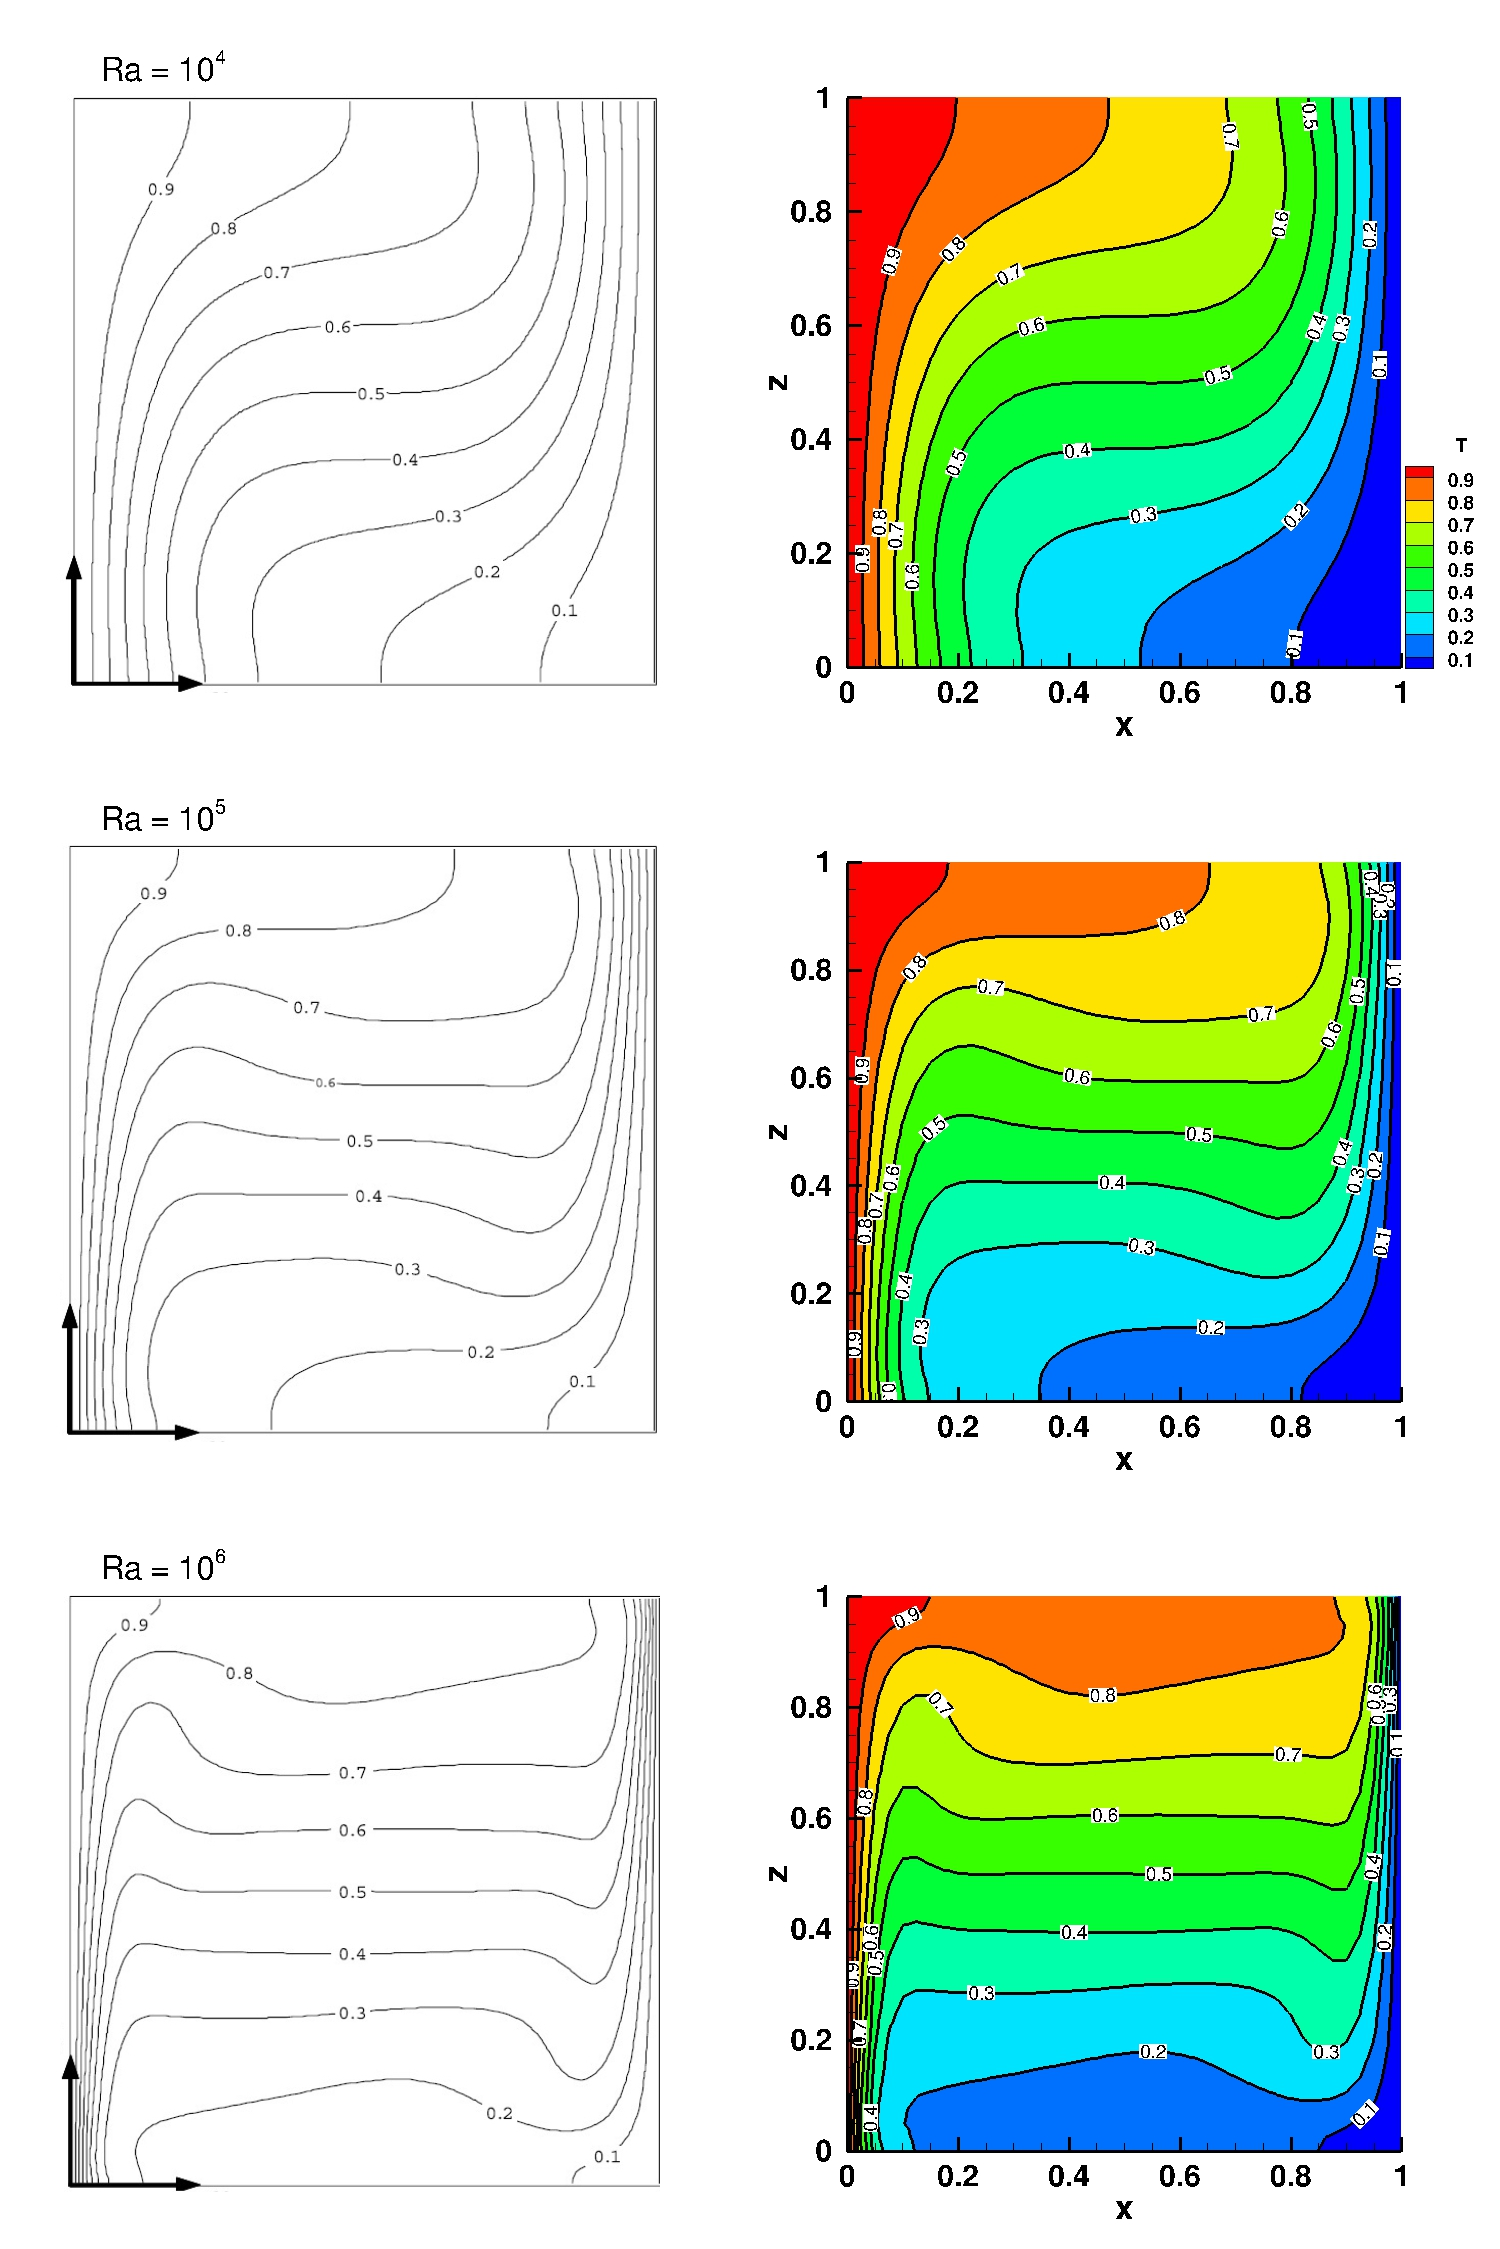
\includegraphics[width=\textwidth]{\figpath/Fig_cap_natconv/Validation_3D_seq_T1}}
\end{center}
\end{minipage}
\caption{3D differentially heated cavity. Temperature contours at the mid-plane of ($y=0.5$); comparison with the results of \cite{Wakashima-2004} (left images). }
\label{fig-3DT} 
\end{figure}


%  1 proc    MatLoc  MatCS   PREC    GMRES   CSolve
%  2 48      6186.33 108.385 61.0397 473.66  2.97339
%  3 96      2468.68 116.805 33.2671 283.099 3.03667
%  4 128     1814.26 116.464 45.5823 237.853 2.74235
%  5 192     1111.5  116.601 25.7295 169.174 2.96447
%  6 240     889.422 123.724 20.8664 146.539 3.03816
%  7 320     674.204 123.723 16.5842 114.346 3.0098
%  8 400     614.418 136.961 14.4055 107.422 3.14586

\subsection{Natural convection in a cube with an inner heated obstacle}\label{sub-OBSTACLE-3D}

The three-dimensional natural convection induced by a temperature difference between a cold outer cubic enclosure is investigated in this section.
Sequential and parallel computation using ffddm are carried out and compared together.

Different Rayleigh numbers varying in the range of $10^4 -10^6$ are considered. The temperature field for $Ra = 10^4$ is reported in Figure \ref{fig-obstacle-Ra1e4} and the Table \ref{tab-T2} shows the error between the sequential and the parallel computation.

\begin{figure}%[!htbp]
\begin{center}
\begin{minipage}{\linewidth}
 {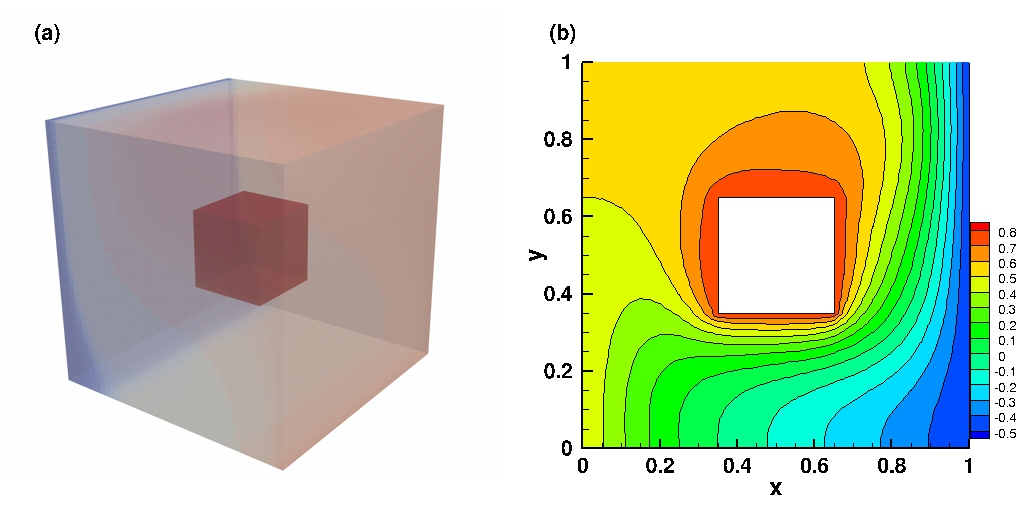
\includegraphics[width=0.98\textwidth]{\figpath/Fig_cap_natconv/3D_OBSTACLE_field}}
\end{minipage}
\end{center}
\caption{3D convection in a cube with an inner heated cube. Temperature fields for $Ra = 10^4$.}
\label{fig-obstacle-Ra1e4} 
\end{figure}

\begin{table}[!h]
	\begin{center}
		\begin{tabular}{|*{7}{c|}}
			\hline
			 Ra & nbseg & nb proc                     & $||u||_{2}$                        & $||u||_{\infty}$                & $||T||_{2}$              & $||T||_{\infty}$\\ \hline \hline
			\multirow{12}{*}{$10^4$} & \multirow{4}{*}{40} & 28 & $0.00087137$ & $0.0058298$ & $ 0.0022491 $ & $0.01592$ \\
			\cline{3-7}
			& & 42 & $0.000870796$ & $0.0058292$ & $ 0.00224866 $ & $0.015921$ \\ \cline{3-7} %\hline 
			& & 56 & $0.000870646$ & $0.0058293$ & $ 0.00224788 $ & $0.015921$  \\ \cline{3-7} %\hline
			& & 70 & $0.000870747$ & $0.0058286$ & $ 0.00224795 $ & $0.015921$ \\ \cline{2-7}
			 & \multirow{4}{*}{60} & 112 & $0.000785593$ & $0.0021$ & $ 0.000858912 $ & $0.010024$ \\% \hline
			\cline{3-7}
			& & 140 & $0.000783164$ & $0.002097$ & $ 0.000865668 $ & $0.010024$ \\ \cline{3-7} %\hline 
			& & 168 & $0.000779419$ & $0.002091$ & $ 0.000858384 $ & $0.010027$  \\ \cline{3-7} %\hline
			& & 196 & $0.000767662$ & $0.00209$ & $ 0.000864693 $ & $0.010019$ \\ \cline{2-7}
			 & \multirow{4}{*}{80} & 224 & $0.000637268$ & $0.001795$ & $ 0.000551538 $ & $0.001661$ \\% \hline
			\cline{3-7}
			& & 238 & $0.000152936$ & $0.000548$ & $ 0.000205031 $ & $0.000634$ \\ \cline{3-7} %\hline 
			& & 252 & $0.000239786$ & $0.000841$ & $ 0.000231648 $ & $0.000661$  \\ \cline{3-7} %\hline
			& & 266 & $0$ & $0$ & $ 0 $ & $0$ \\ \hline 
			\multirow{12}{*}{$10^5$}& \multirow{4}{*}{40} & 28 & $0.0011359$ & $0.0089746$ & $ 0.00401922 $ & $0.020067$ \\% \hline
			\cline{3-7}
			& & 42 & $0.00113742$ & $0.0089788$ & $ 0.00402103 $ & $0.020067$  \\ \cline{3-7} %\hline 
			& & 56 & $0.00113625$ & $0.0089768$ & $ 0.00402081 $ & $0.020063$   \\ \cline{3-7}%\hline
			& & 70 & $0.0011348$ & $0.0089726$ & $ 0.00401999 $ & $0.020065$  \\ \cline{2-7} %\hline
			 & \multirow{4}{*}{60} & 112 & $0.000765582$ & $0.0022345$ & $ 0.00166687 $ & $0.015296$ \\% \hline
			\cline{3-7}
			& & 140 & $0.000763449$ & $0.0022313$ & $ 0.00166143 $ & $0.015257$ \\ \cline{3-7} %\hline 
			& & 168 & $0.000763074$ & $0.0022176$ & $ 0.00166605 $ & $0.015284$  \\ \cline{3-7} %\hline
			& & 196 & $0.000760368$ & $0.0022093$ & $ 0.00167368 $ & $0.015299$ \\ \cline{2-7} 
			 & \multirow{4}{*}{80} & 224 & $0.00051462$ & $0.0016627$ & $ 0.000574467 $ & $0.001794$ \\% \hline
			\cline{3-7}
			& & 238 & $5.17443 \times 10^{-05}$ & $0.0001934$ & $ 0.00018074 $ & $0.0005666$ \\ \cline{3-7} %\hline 
			& & 252 & $8.68245 \times 10^{-05}$ & $0.000319$ & $ 8.11788 \times 10^{-05} $ & $0.000335$  \\ \cline{3-7} %\hline
			& & 266 & $0$ & $0$ & $ 0 $ & $0$ \\ \hline 

		\end{tabular}
	\end{center}
	\caption {3D convection in a cube with an inner heated cube. Comparison between sequential and ffddm algorithm for uniform grids of $40 \times 40 \times 40$ for $Ra = 10^4$ and $80 \times 80 \times 80$ for $Ra = 10^5$}
	\label{tab-T2}
\end{table}

%The study investigated the effect of the inner sphere location on the heat transfer and fluid flow. A schematic of the three-dimensional domain is presented in figure \ref{fig-cerc_3D}. 
%\begin{figure}[!htbp]
%\begin{minipage}{1.\linewidth}
%\begin{center}
% {\includegraphics[width=0.6\textwidth]{\figpath/figs_Raluca_thesis/cap_5/grafic_C3D.jpg}}\\
%\end{center}
%\end{minipage}
%\caption{Computational domain and boundary conditions for a 3D convection problem with a spherical obstacle.}
%\label{fig-cerc_3D} 
%\end{figure}
%
%%The flow and termal fields eventually reach the steady state for all Rayleigh numbers regardless of the sphere location.
%No-slip boundary conditions are imposed on the walls for the velocity field. The walls are isothermal, of temperature $T=0$, while the inner sphere temperature is $T=1$. The flow and thermal fields converge towards a steady state for all Rayleigh numbers.  
%
%Figure \ref{fig-cerc_iso} presents the isotherms and streamlines obtained by \cite{Yoon-2010} for Rayleigh numbers varying from $10^4$ to $10^6$. 
%\begin{figure}[!htbp]
%\begin{minipage}{1.\linewidth}
%\begin{center}
%$Ra=10^4$\\
% {\includegraphics[width=0.5\textwidth]{\figpath/figs_Raluca_thesis/cap_5/grafic_C3D_Ra1e4.jpg}}
%\end{center}
%\end{minipage}
%\begin{minipage}{1.\linewidth}
%\begin{center}
% $Ra=10^5$\\
% {\includegraphics[width=0.5\textwidth]{\figpath/figs_Raluca_thesis/cap_5/grafic_C3D_Ra1e5.jpg}}
%\end{center}
%\end{minipage}
%\begin{minipage}{1.\linewidth}
%\begin{center}
%$Ra=10^6$\\
% {\includegraphics[width=0.5\textwidth]{\figpath/figs_Raluca_thesis/cap_5/grafic_C3D_Ra1e6.jpg}}
%\end{center}
%\end{minipage}
%\caption{3D convection problem with a spherical obstacle. Isotherms and streamlines for three different $Ra$ numbers.  Results of \cite{Yoon-2010}.}
%\label{fig-cerc_iso} 
%\end{figure}
%
%
%%%\clearpage
%
%Figure \ref{fig-cerc_ra6} shows the same maps obtained with our numerical code.  For $\Ray=10^4$, the effect of convection on heat transfer is low forming a weak upward thermal plume on the top of the sphere.  The thermal boundary layer on the bottom part of sphere is thinner than that on the upper side. The circulation in the upper part of the enclosure is more active, resulting in the formation of one inner recirculation cell.
%
%
%For $Ra=10^5$ convection is predominant with respect to conduction,  as shown in figure \ref{fig-cerc_ra6}. A plume forms on top of the inner sphere which gives rise to stronger thermal gradient on the top of the enclosure. The dominant flow is in the upper half of the enclosure, and correspondingly the center of the recirculating cell is located in the upper half. %The flow at the bottom of the enclosure is weak compared with that the middle and top regions suggesting a stratification effect in the lower part of the cavity.
%
%
%For $\Ray=10^6$, the isotherms are distorted  due to the stronger convection effects thus having a stable stratification of isotherms.
%The convection velocity increases with increasing Rayleigh number, the boundary layer behaviour can be seen in the lower part regions of the sphere and the upper part of the enclosure. The plume arising form the sphere separates as it reaches the top wall. The centres of the inner recirculation cells move toward the upper corners. 
%
%
%\begin{figure}[!htbp]
%$Ra=10^4$\\
%\begin{minipage}{0.32\linewidth}
%\begin{center}
% {\includegraphics[width=1.\textwidth]{\figpath/figs_Raluca_thesis/cap_5/Ra1e4_3.jpg}}\\
% \end{center}
%\end{minipage}
%\begin{minipage}{0.32\linewidth}
%\begin{center}
% {\includegraphics[width=1.\textwidth]{\figpath/figs_Raluca_thesis/cap_5/Ra1e4_7.jpg}}\\
%\end{center}
%\end{minipage}
%\begin{minipage}{0.32\linewidth}
%\begin{center}
% {\includegraphics[width=1.\textwidth]{\figpath/figs_Raluca_thesis/cap_5/Ra1e4_9.jpg}}\\
%\end{center}
%\end{minipage}
%
%$Ra=10^5$\\
%\begin{minipage}{0.32\linewidth}
%\begin{center}
% {\includegraphics[width=1.\textwidth]{\figpath/figs_Raluca_thesis/cap_5/Ra1e5_4.jpg}}\\
%\end{center}
%\end{minipage}
%\begin{minipage}{0.32\linewidth}
%\begin{center}
% {\includegraphics[width=1.\textwidth]{\figpath/figs_Raluca_thesis/cap_5/Ra1e5_7.jpg}}\\
%\end{center}
%\end{minipage}
%\begin{minipage}{0.32\linewidth}
%\begin{center}
% {\includegraphics[width=1.\textwidth]{\figpath/figs_Raluca_thesis/cap_5/Ra1e5_9.jpg}}\\
%\end{center}
%\end{minipage}
%
%
%$Ra=10^6$\\
%\begin{minipage}{0.32\linewidth}
%\begin{center}
% {\includegraphics[width=1.\textwidth]{\figpath/figs_Raluca_thesis/cap_5/Ra1e6_3.jpg}}\\
%\end{center}
%\end{minipage}
%\begin{minipage}{0.32\linewidth}
%\begin{center}
% {\includegraphics[width=1.\textwidth]{\figpath/figs_Raluca_thesis/cap_5/Ra1e6_7.jpg}}\\
%\end{center}
%\end{minipage}
%\begin{minipage}{0.32\linewidth}
%\begin{center}
% {\includegraphics[width=1.\textwidth]{\figpath/figs_Raluca_thesis/cap_5/Ra1e6_9.jpg}}\\
%\end{center}
%\end{minipage}
%\caption{3D convection problem with a spherical obstacle. Present study. Isotherms and streamlines for different Rayleigh numbers.}
%\label{fig-cerc_ra6} 
%\end{figure}
%
%We can conclude that the results obtained with our FD+IBM method for the 3D case  are in good agreement with the test case considered, rendering possible the simulation of 3D configurations with obstacles of general geometries.


%\subsection{Note on parameters for ffddm and Newton method}\label{ffddm-param}
%In this section, we only focus on natural or mixed convection, without phase changing. The system of non-linear equations (\ref{eq-weak-all}) is solved using a Newton method. We have tested two ways of solving this non linear problem. Rewriting the problem as 
%$$
%F(U) = 0,
%$$
%Newton method can be implemented in any of the two following ways:\begin{itemize}
%\item Start with initial guess $U^{(0)}$ and compute $W$ from:
%$$
%W = DF(U^{(k)})^{-1}\ F(u^{(k)}).
%$$
%Then, update $U^{(k+1)} = U^{(k)}-W$.
%\item Start with initial guess $U^{(0)}$ and directly compute $U^{(k+1)}$ from:
%\begin{equation}\label{eq:newton_approach}
%U^{(k+1)} = DF(U^{(k)})^{-1}\left( DF(U^{(k)}) U^{(k)} - F(U^{(k)})\right).
%\end{equation}
%\end{itemize}
%We choose the latter \eqref{eq:newton_approach} for several reasons: for example, the right hand side and time-dependent boundary conditions (when applicable) are easier to implement. Moreover, ffddm uses algebraic norms to compute residuals, thus making the norms mesh dependent. It is then natural to use the iterative solver of ffddm with relative tolerance. This relative error is based on the right hand side. In the first case, this norm will decrease so that it is difficult to set up a good criterion. In the latter, we expect very few variations in the amplitude of the successive RHS.
%
%Eventually, at each Newton iteration, we have to solve linear problems of the kind: start with $(u^{(0)},p^{(0)},\theta^{(0)})=(u_n,p_n,\theta_n)$, and find $(u^{(k+1)},p^{(k+1)},\theta^{(k+1)})$ from
%\begin{align*}
%cdt\ u^{(k+1)} + u^{(k)}\nabla u^{(k+1)} + u^{(k+1)}\nabla u^{(k)} &- IRe\Delta u^{(k+1)} + \nabla p^{(k+1)} - IRe\;cc\;\theta^{(k+1)} e_y \\
%&= u^{(k)}\nabla u^{(k)}  + cdt\ u_n, \\
%\nabla\cdot u^{(k+1)} + \epsilon p^{(k+1)} &= 0, \\
%cdt\ \theta^{(k+1)} + u^{(k)}\nabla\theta^{(k+1)} + u^{(k+1)}\nabla\theta^{(k)} -IPr\Delta \theta^{(k+1)} &= u^{(k)}\nabla\theta{(k)} + cdt\ \theta_n
%\end{align*}
%
%$\epsilon$ is a penalty term with very small value ($\epsilon=1.e-7$), $cdt$ is $1/{\delta t}$ (resp. 0) in the unsteady problem (resp. stationary cases). $cc=1$ for unsteady problems. For stationary problems, we solve the problems for different values of $cc$, from $0$ to $1$. The reason is that the original problem ($cc=1$) can be difficult to approximate with Newton's method. By changing this parameter, we hope to start with a suitable initial guess, so that the method may converge.
%
%For stationary solutions, we recommend the use of the following parameters:
%\begin{itemize}
%\item tolerance in Newton's iterations: for the first steps ($cc<1$), use $1.e-3$; for the last step ($cc=1$), use a tolerance less than $1.e-6$,
%\item relative tolerance in ffddm: $1.e-9$,
%\item maximum number of iterations for ffddm: at least 400, but this can change according to the problem (usually I put 2000 to be sure), especially for 3D problems: need to test influence of the number of procs on the number of iterations needed by GMRES.
%\end{itemize}
%
%For time dependent solutions, we recommend the use of the following parameters:
%\begin{itemize}
%\item tolerance in Newton's iterations: use a tolerance less than $1.e-6$,
%\item relative tolerance in ffddm: $1.e-9$,
%\item if we want to approximate a steady solution with the unsteady scheme, we set a tolerance $\epsilon_{conv}$ on the residuals. It must be consistent with the tolerance for Newton's iterations, e.g. $\epsilon_{conv}>\epsilon_{Newton}$.
%\end{itemize}
%
%Finally, there is an issue with ffddm in 3D for some configurations, e.g. natural convection in a cube without the central sphere. This issue has been partially fixed if we use the develop version in \\
%\url{https://github.com/FreeFem/FreeFem-sources/tree/develop}.
%
%In order to have a working set up, the following changes have to be made with this latest release of ffddm:\begin{itemize}
%\item The command \verb?scaledExchange(A,rhs)? does no longer exist: it must be replaced by \verb?exchange(A,rhs,scaled=true)?,
%\item This fix works only with pure Dirichlet BC: we have to use $tgv=-1$ in FF++\begin{verbatim}
%Mat = vPb(WhAugmented, WhAugmented,tgv=-1);
%rhsFull = vM(0, WhAugmented,tgv=-1);
%\end{verbatim}
%\end{itemize}

%\subsection{Scalability with ffddm}
%
%\begin{figure}[h]
%   \begin{center}
%      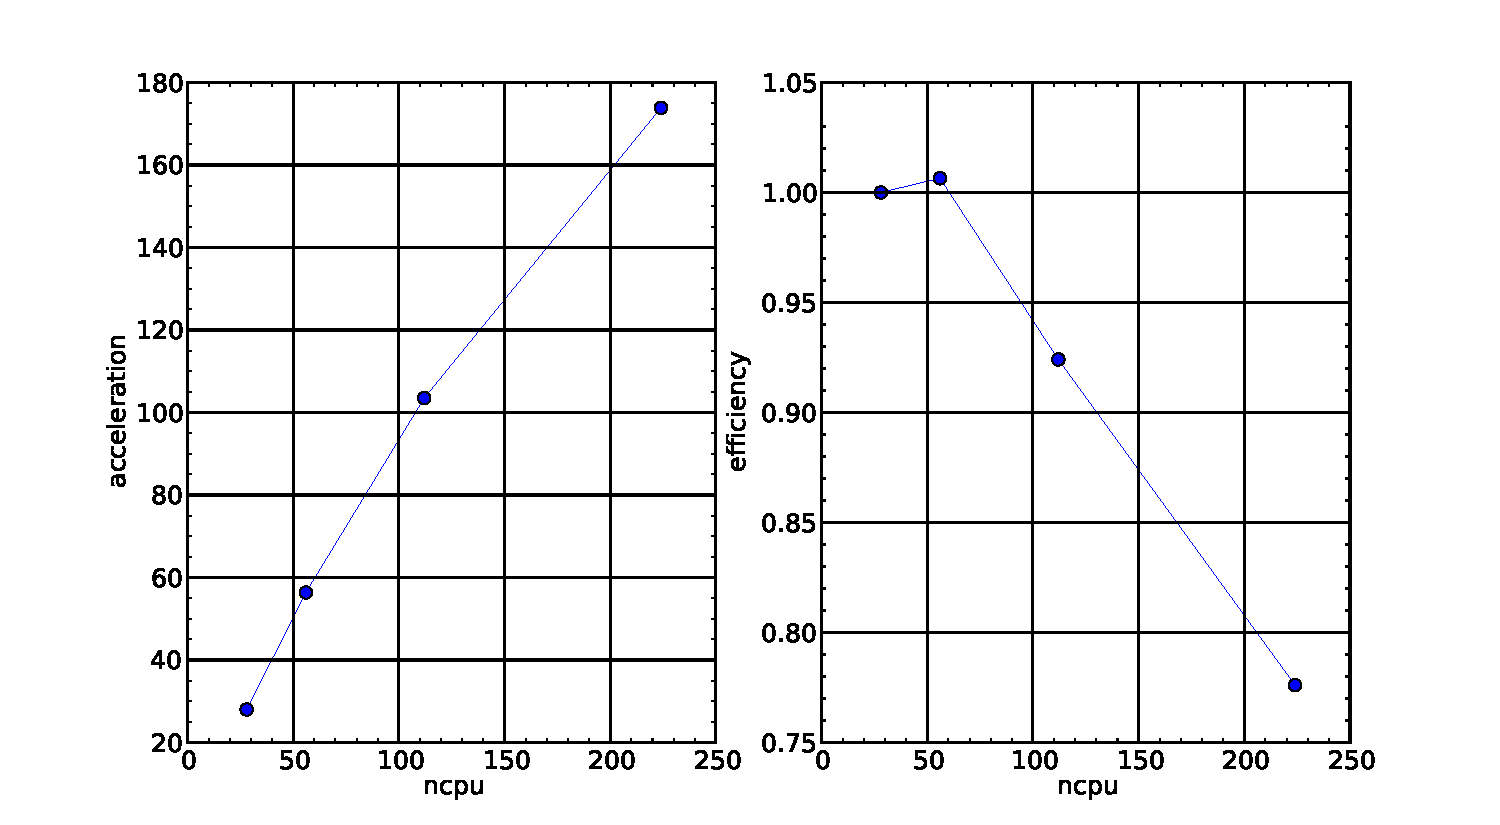
\includegraphics[width=0.49\textwidth]{\figpath/Fig_cap_natconv/Sta_3d_40_scalability.pdf}
%      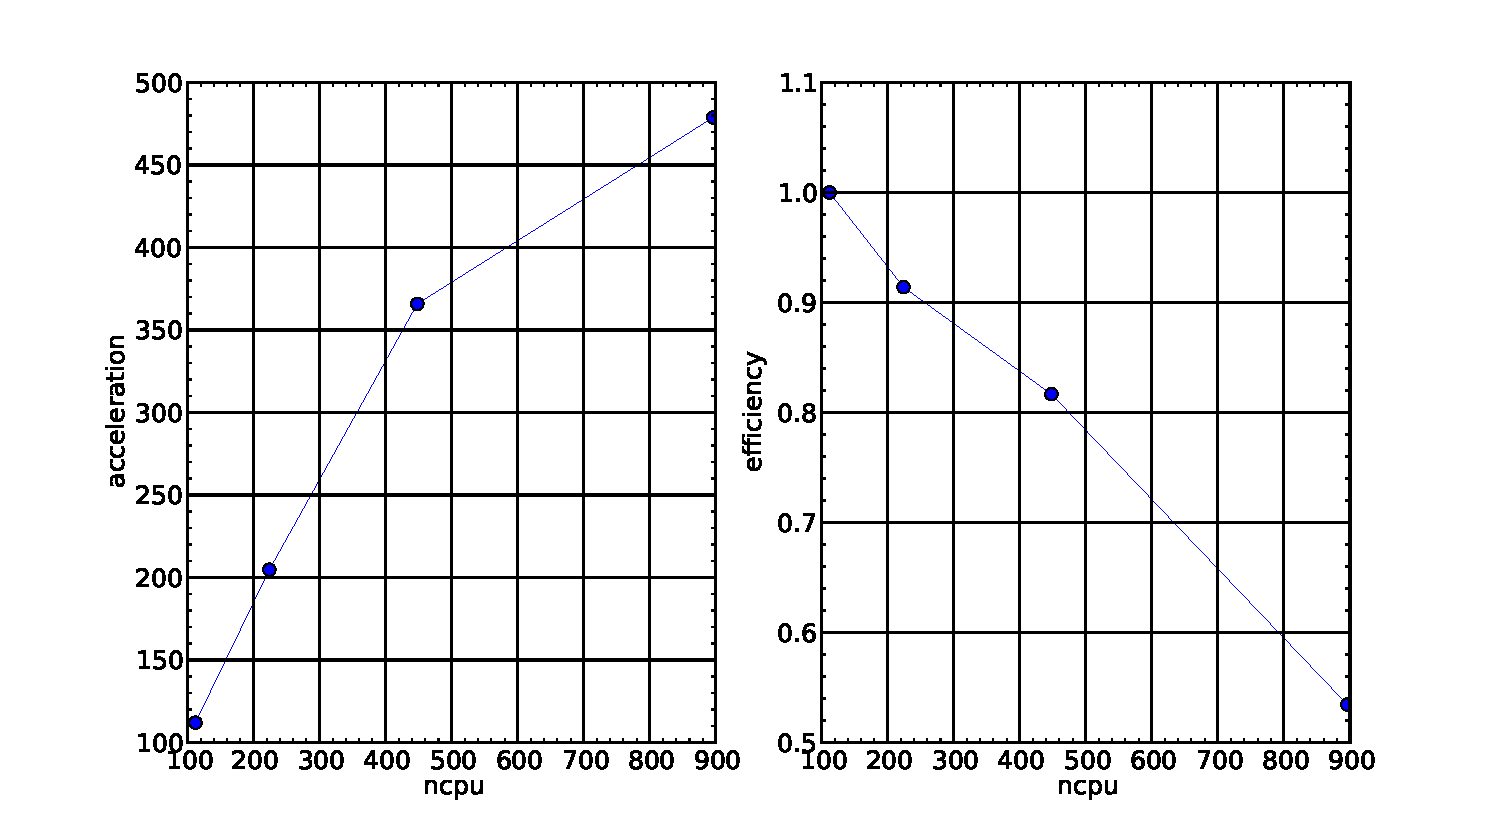
\includegraphics[width=0.49\textwidth]{\figpath/Fig_cap_natconv/Sta_3d_60_scalability.pdf}\\
%      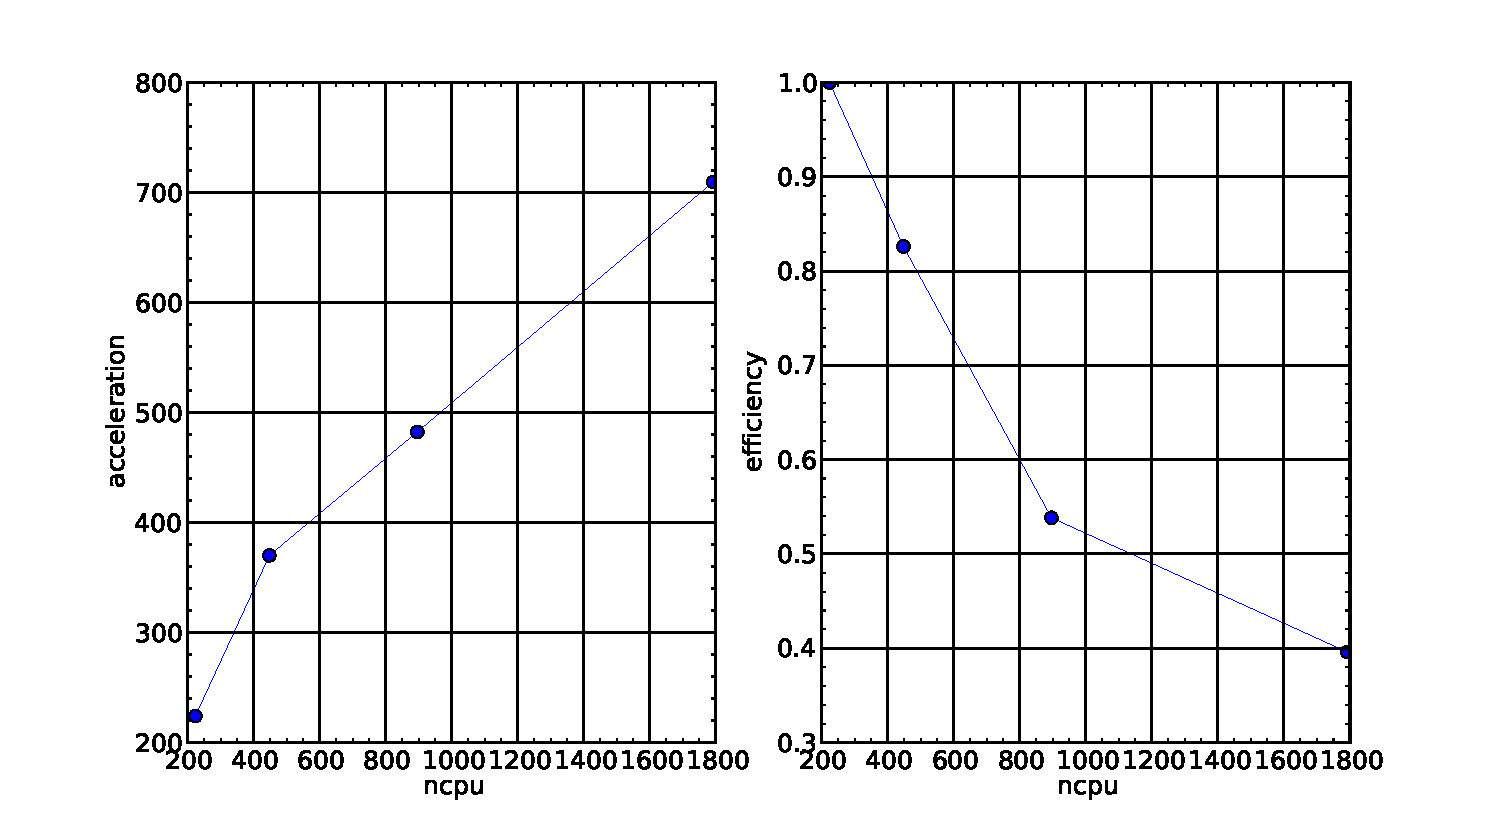
\includegraphics[width=0.49\textwidth]{\figpath/Fig_cap_natconv/Sta_3d_80_scalability.pdf}
%   \end{center}
%   \caption{scalability for a discretisation of $40\times 40$, $60\times 60$ and $80\times 80$}
%   \label{fig-sca_3d_40}
%\end{figure}
%
%\begin{figure}[h]
%   \begin{center}
%      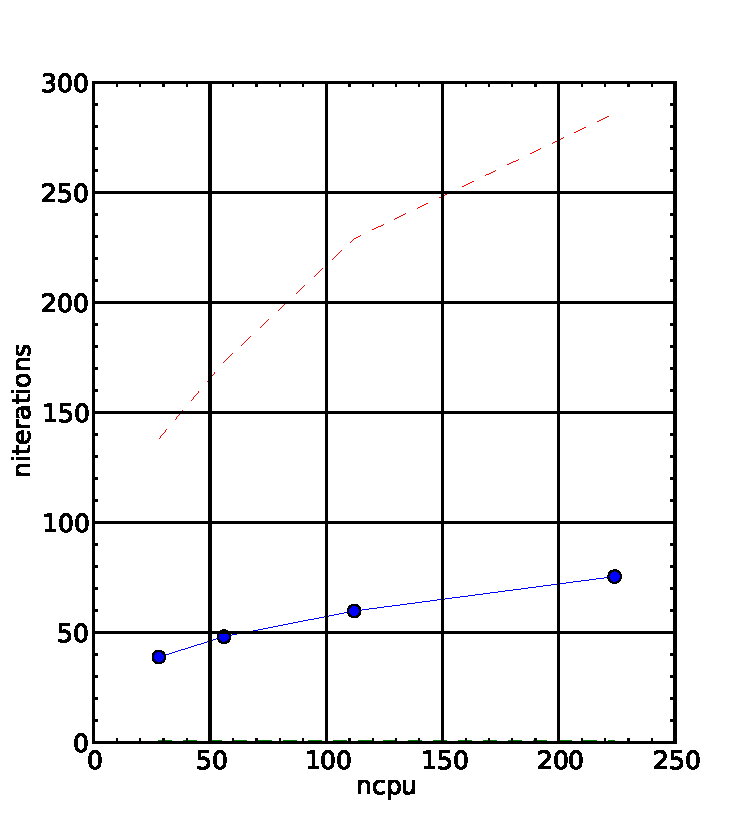
\includegraphics[width=0.3\textwidth]{\figpath/Fig_cap_natconv/Sta_3d_40_gmres.pdf}
%      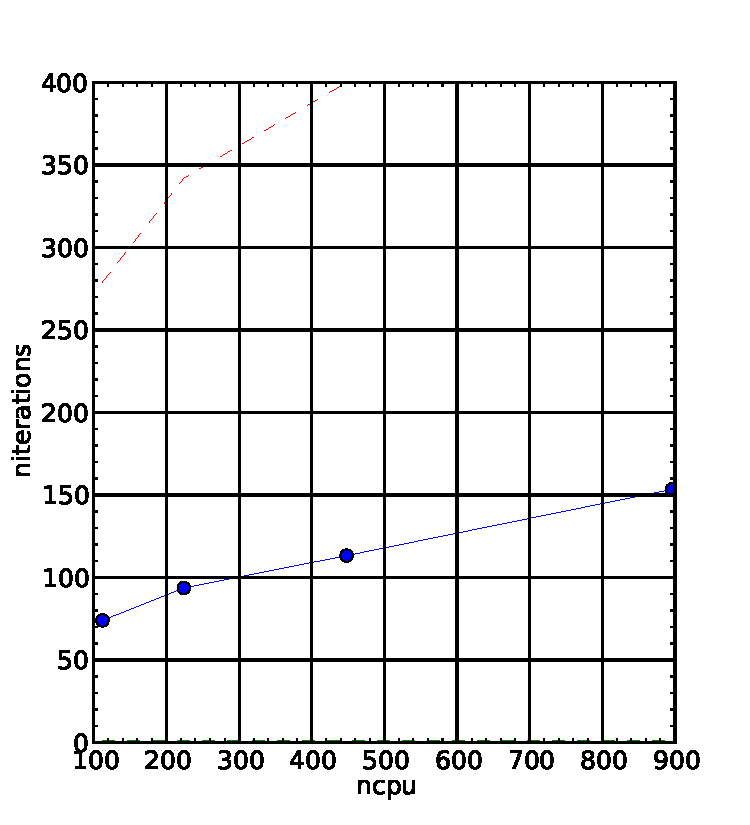
\includegraphics[width=0.3\textwidth]{\figpath/Fig_cap_natconv/Sta_3d_60_gmres.pdf}
%      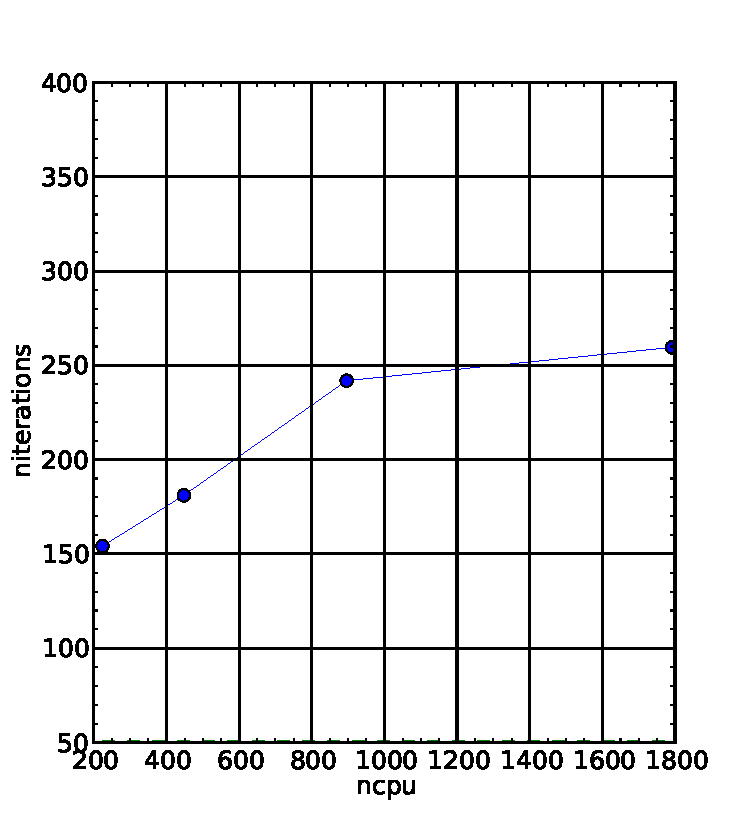
\includegraphics[width=0.3\textwidth]{\figpath/Fig_cap_natconv/Sta_3d_80_gmres.pdf}
%   \end{center}
%   \caption{GMRES iterations for a discretisation of $40\times 40$, $60\times 60$ and $80\times 80$}
%   \label{fig-sca_3d_40}
%\end{figure}




\graphicspath{{\figpath/Fig_cap_melting}}
%%%%%%%%%%%%%%%%%%don't forget if needed %%%%%%%%%%%%%%%%%%%%%
%\section[toc version]{title version%
%              \sectionmark{head version}}
%\sectionmark{head version}
%%%%%%%%%%%%%%%%%%%%%%%%%%%%%%%%%%%%%%%%%%%%%%%%%%%%%%%%%%%%%%
\def\titcourt{Numerical simulations of phase change material}
\def\titlong{Numerical simulation of phase change Materials in 2D configurations}
%%%%%%%%%%%%%%%%%%%%%%%%%%%%%%%%%%%%%%%%%%%%%%%%%%%%%%%%%%%%%%%%
\chapter[\titlong]{\titlong%
              \chaptermark{\titcourt}}
\chaptermark{\titcourt}
\label{chap-MELTING}
%%%%%%%%%%%%%%%%%%%%%%%%%%%%%%%%%%%%%%%%%%%%%%%%%%%%%%%%%%%%%%%%
%%%%%%%%%%%%%%%%%%%%%%%%%%%%%%%%%%%%%%%%%%%%%%%%%%%%%%%%%%%%%%%%

%Having proven the accuracy and the efficiency of our numerical method by simulating the Navier-Stokes-Boussinesq equations, we now pay a closer attention to convective phase-change problems.
The purpose of this chapter is to validate our numerical method by simulating convective phase-change problems.
A discussion on numerical parameters is given first followed, by a sequence of validations computing different physical and geometrical configurations.

The Newton algorithm in Eq. \eqref{eq-newton-C1} is now solved throughout the whole domain containing liquid and solid phases.
When compared to the previous validation, two new non-linearities are now added: the Carman-Kozeny penalty term in the momentum equation and the enthalpy source term in the energy equation.
The Carman-Kozeny penalty term is used to ensure zero velocity in the solid region and 
the enthalpy non-linear source term is included to model the phase-change in the energy equation.
Following the same idea as in the natural convection validation cases in Chapter \ref{chap-NATCONV}, the non-linearity in the body force is gradually added.
We consider first the linear form of $f_B(\theta)$ by investigating the melting of various PCM within several shapes of the containers.
Then, the challenging case of water freezing, characterized by a non-linear variation of the density (see Eq. \eqref{eq-dens-nonlin} in Chapter \ref{chap-NATCONV}), is simulated.

Details about the parameter settings are first given in Sec. \ref{sec-param-set}:
the characteristics of the mushy-zone, the mesh adaptivity and the initial condition are discussed in details.
Second, the melting of n-octadecane and Gallium are presented in Secs. \ref{sec: melting-2D} and \ref{sec-melt-gallium}.
The physical properties of n-octadecane and Gallium used in our simulations are reported in Tab. \ref{tab-param-PCM}.
\begin{table}[!ht]
   \begin{center}
      \begin{tabular}{*{8}{cl}}
         
        &$\rho$ &$ \mu$ & $h_{SL}$ & $c_p $ & $k$ & $T_f$ & $\beta$ \\
        &kg/m$^3$ & kg/(m s) & kJ/kg & J/(kg K) & W/(m K) & K & 1/K \\
         \hline
        Octadecane & 774 & 3.9 $\cdot 10^{-3}$  & 244 & $2180$ & $0.152$ & $301$ & 8.5 $\cdot 10^{-4}$ \\
        Gallium & 6093 & 1.81 $\cdot 10^{-3}$  & 80.16 & $381.5$ & $32$ & $301$ & 1.2 $\cdot 10^{-4}$ \\
      \end{tabular}
   \end{center}
   \caption{Physical properties of n-octadecane and Gallium PCM.}
   \label{tab-param-PCM}
\end{table}



\noindent Then, in Secs. \ref{subsec-luo} and \ref{sec-solid-crust} we demonstrate the capability of our code to deal with different shape of the domain.
The melting of a cylindrical PCM with inner heated tubes is presented in Sec. \ref{subsec-luo} and the solid crust formation in a highly distorted mesh is carried out in Sec. \ref{sec-solid-crust}.
Finally, the water freezing case is performed in Sec. \ref{sec-water-freeze}.
Besides the non-linear definition of the body force, the striking feature of the water freezing simulation is the tracking of several interfaces, namely the solidification front and the anomalous thermal variation of density. 
Our result is qualitatively compared with the experimental results of \cite{Kowalewski-1999}.

%\newpage
\section{Parameter settings} \label{sec-param-set}
We present in this section the setting of the main numerical parameters. 
The influence of the penalty term $A(\theta)$ in the momentum equation is discussed first, namely the value of the Carman-Kozeny constant $\CKC$.
Second, details about the mesh adaptivity parameters are given.

\subsection{Carman-Kozeny constant}
The Carman-Kozeny penalty term is used to annihilate the velocity in the solid region when a single domain method is applied.
The Carman-Kozeny constant $\CKC$, appearing in Eq. \eqref{eq-CK} accounts for the mushy-region morphology.
The effect of this constant on the melting and the solidification processes have attracted some attention in the literature.
Even though it is generally assumed that a large value for $\CKC$ must be set, the exact value of this constant could influence the accuracy of the results. % \citep{kheirabadi2015effect, Kumar2017}. \\

\noindent The influence of $\CKC$ in the location of the solid-liquid front was investigated by \cite{kheirabadi2015effect}.
They have concluded that high $\CKC$ values induce a slower melting rates, and conversely small values result in unphysical predictions of the melting front development.
They also noticed that $\CKC$ and the melting temperature range $\Delta T_{\varepsilon} = T_{\varepsilon2}-T_{\varepsilon1}$ are dependent of one another: different values of $\Delta T_{\varepsilon}$ require different values of $\CKC$ to obtain the same melting front location.

\noindent \cite{Kumar2017} studied the effect of the mushy zone constant and its influence on the melt fraction, vortex strength and the amount of heat storage. They have shown that increasing $\CKC$ leads to a decrease of the convection strength and consequently to a decrease of the heat transfer rate. 
These studies show the necessity of choosing an appropriate value of this parameter. 
Because of the semi-solid state and porous nature of the mushy zone, the choice of the value of this constant is still an open problem.

To assess on the influence of the Carman-Kozeny constant, we simulate the melting of a n-octadecane PCM within rectangular enclosures with the following dimensionless parameters: $\Ray = 3.27 \cdot 10^5$, $\Prd = 56.2$ and $\Ste = 0.045$.
Different value of $\CKC$ are used ranging from $10^6$ to $10^{10}$. We compare the location of the melting front with the experimental data of \cite{Okada1984}.
Figure \ref{fig:pcm-CK} displays the location of the phase-change interface for three values of $\CKC$: $10^6$, $10^8$ and $10^{10}$.
Very good agreement with the experimental result of \cite{Okada1984} is obtained for $\CKC$ varying in the range $[10^6, 10^8]$. 
Imposing  a too large value, $\CKC=10^{10}$, results  in artificially slowing the propagation of the melting front. 

The local liquid fraction function $L_f(\theta)$ is regularized through the artificial mushy zone as following:
\begin{equation}
L_f(\theta) = 1 - \frac{1}{2}\left\{
1 + \tanh\left(\frac{\theta_{ck}-\theta}{R_{ck}}\right)
\right\}.
\label{eq-Lf-CK}
\end{equation}

\noindent The value of $\theta_{ck}$ is set in order to have the sharp variation of the derivative of d$L_f/$d$\theta$ near the new phase appearing in the system, i.e. liquid for melting ($\theta_{ck}=\varepsilon$), and solid  for freezing ($\theta_{ck}=\theta_f$) (see also \cite{dan-2014-JCP}).
This is to ensure that the velocity in the solid region is correctly set to $\vec u = 0$.
As far as $R_{ck}$ is concerned, several values ranging from $\varepsilon$ to $\varepsilon/4$ were tested and
we set for all subsequent simulations $\CKC= 10^6$ and $R_{ck} = \varepsilon$.

\begin{figure}
	\begin{center}
		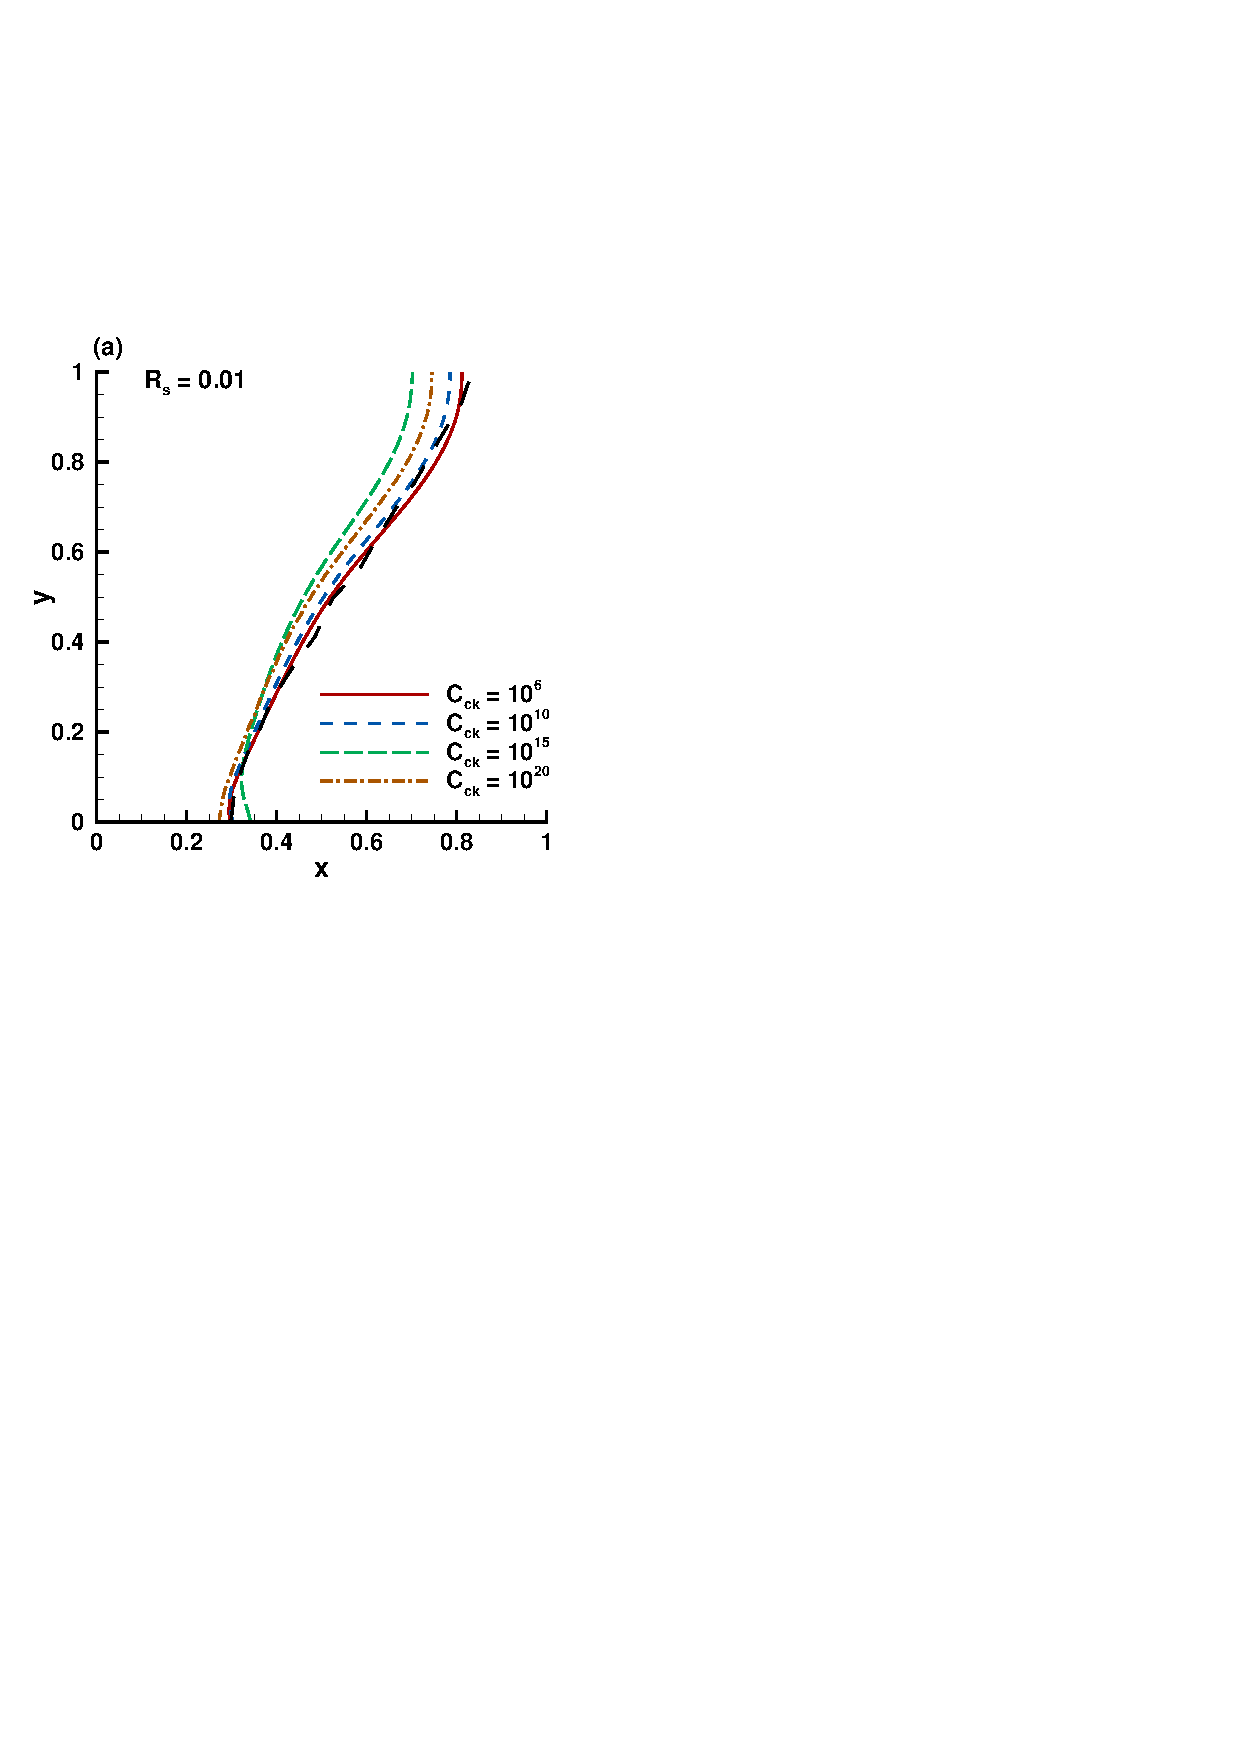
\includegraphics[width=.5\textwidth]{\figpath/Fig_cap_melting/PCM_ck_compare}
	\end{center}
	\caption{Location of the interface during the melting of the PCM using different value of $\CKC$ ranging from $10^6$ to $10^{10}$. Comparison with experimental data of \cite{Okada1984}}
	\label{fig:pcm-CK}
\end{figure}

%\newpage
%\clearpage
\subsection{Mesh adaptativity}

The use of mesh adaptation proved mandatory in the present simulation of PCM melting to obtain accurate results within reasonable computational time.
For the melting case, we used five metrics intersection to adapt the mesh, based on $S^{n+1}, S^{n}, T^{n+1}, T^{n},$ and $\vec{u}^{n+1}$. To reduce the impact of the interpolation on the global accuracy for time-depending problems, we consider the metrics computed from actual (at $t_{n+1}$) and  previous (at $t_{n}$) values, for the same variable used for adaptivity (see also \cite{Belhamadia2004_S}).

\noindent The mesh adaptation strategy requires to set  the interpolation error level {\em errh}, the minimum and the maximum edge sizes {\em hmin} and {\em hmax}, and the {\em adaptratio} parameter, which defines the ratio for a prescribed smoothing of the metric.
The minimum size of triangles and the interpolation error level are set in order to capture the smaller length scale, mainly the boundary layer structures close to the wall, and to solve accurately the large gradient at the solid-liquid interfaces.
The error level is adapted for each variable on which the metric is computed.
A default value {\em errh = 0.02} is defined for $T$ and $\vec{u}$, and {\em errh = 0.2} for $S$.
%Furthermore, {\em hmin} should be set in order to capture the smaller length scale, mainly the boundary layer structures close to the wall, and to solve accurately the large gradient at the solid-liquid interfaces.
The scale for boundary layers in natural convection flow along a vertical wall is given by Eq. \eqref{eq-bnd-layer-T}. % and \ref{eq-corr-Low-Pr}.
For high-Prandtl simulations, the thickness of the thermal boundary layer is thinner than the viscous boundary layers, and conversely for low-Prandtl fluid the viscous boundary layer is thinner than the thermal one.
In our simulations, Rayleigh numbers in the range of $10^6$ to $10^8$ and Prandtl number of order of $50$, lead to a dimensionless thickness of the thermal boundary layer of order of $\delta_\theta \sim 10^{-3}$.
%Conversely, for low-Prandtl simulations the viscous boundary layer is thinner than the thermal boundary layer.
For the same range of Rayleigh numbers and Prandtl number of order of $0.1$, we have a dimensionless thickness of the viscous boundary layer of $\delta_\nu \sim 10^{-2}$. 
The minimum edge-length is therefore set to $hmin = 10^{-3}$.
Moreover, we fixe the maximum triangle size to avoid generating too large number of nodes. %, and we impose also the anisotropy of the mesh to have value close to $1$.
%The optimal parameters for the mesh adaptivity are given in Tab. \ref{tab-param-mesh}.
%\begin{table}
%   \begin{center}
%      \begin{tabular}{*{5}{cl}}
%               	hmin & hmax & adaptratio & errh & nbvx \\
%         	\hline
%         	$10^{-3}$ & $0.1$ & $1.5$ & $0.01$ & $50,000$ \\
%      \end{tabular}
%   \end{center}
%   \caption{Parameters for the mesh adaptivity.}
%   \label{tab-param-mesh}
%\end{table}
%Moreover, a minimum of 8 triangles should be included in the mushy zone to ensure an accurate location of the melting interface and a correct resolution of gradients.

%minimum edge-length is set to $h_{min} = 10^{-3}$ and the maximum edge-lenght to $h_{max} = 0.1$.
%Two values  \texttt{errh} $= 10^{-1}$ and \texttt{errh} $= 10^{-2}$, are computed and the corresponding meshes at $t=78.8$ are displayed in Fig. (FIG MAILLAGE).

\begin{figure}
	\begin{center}
		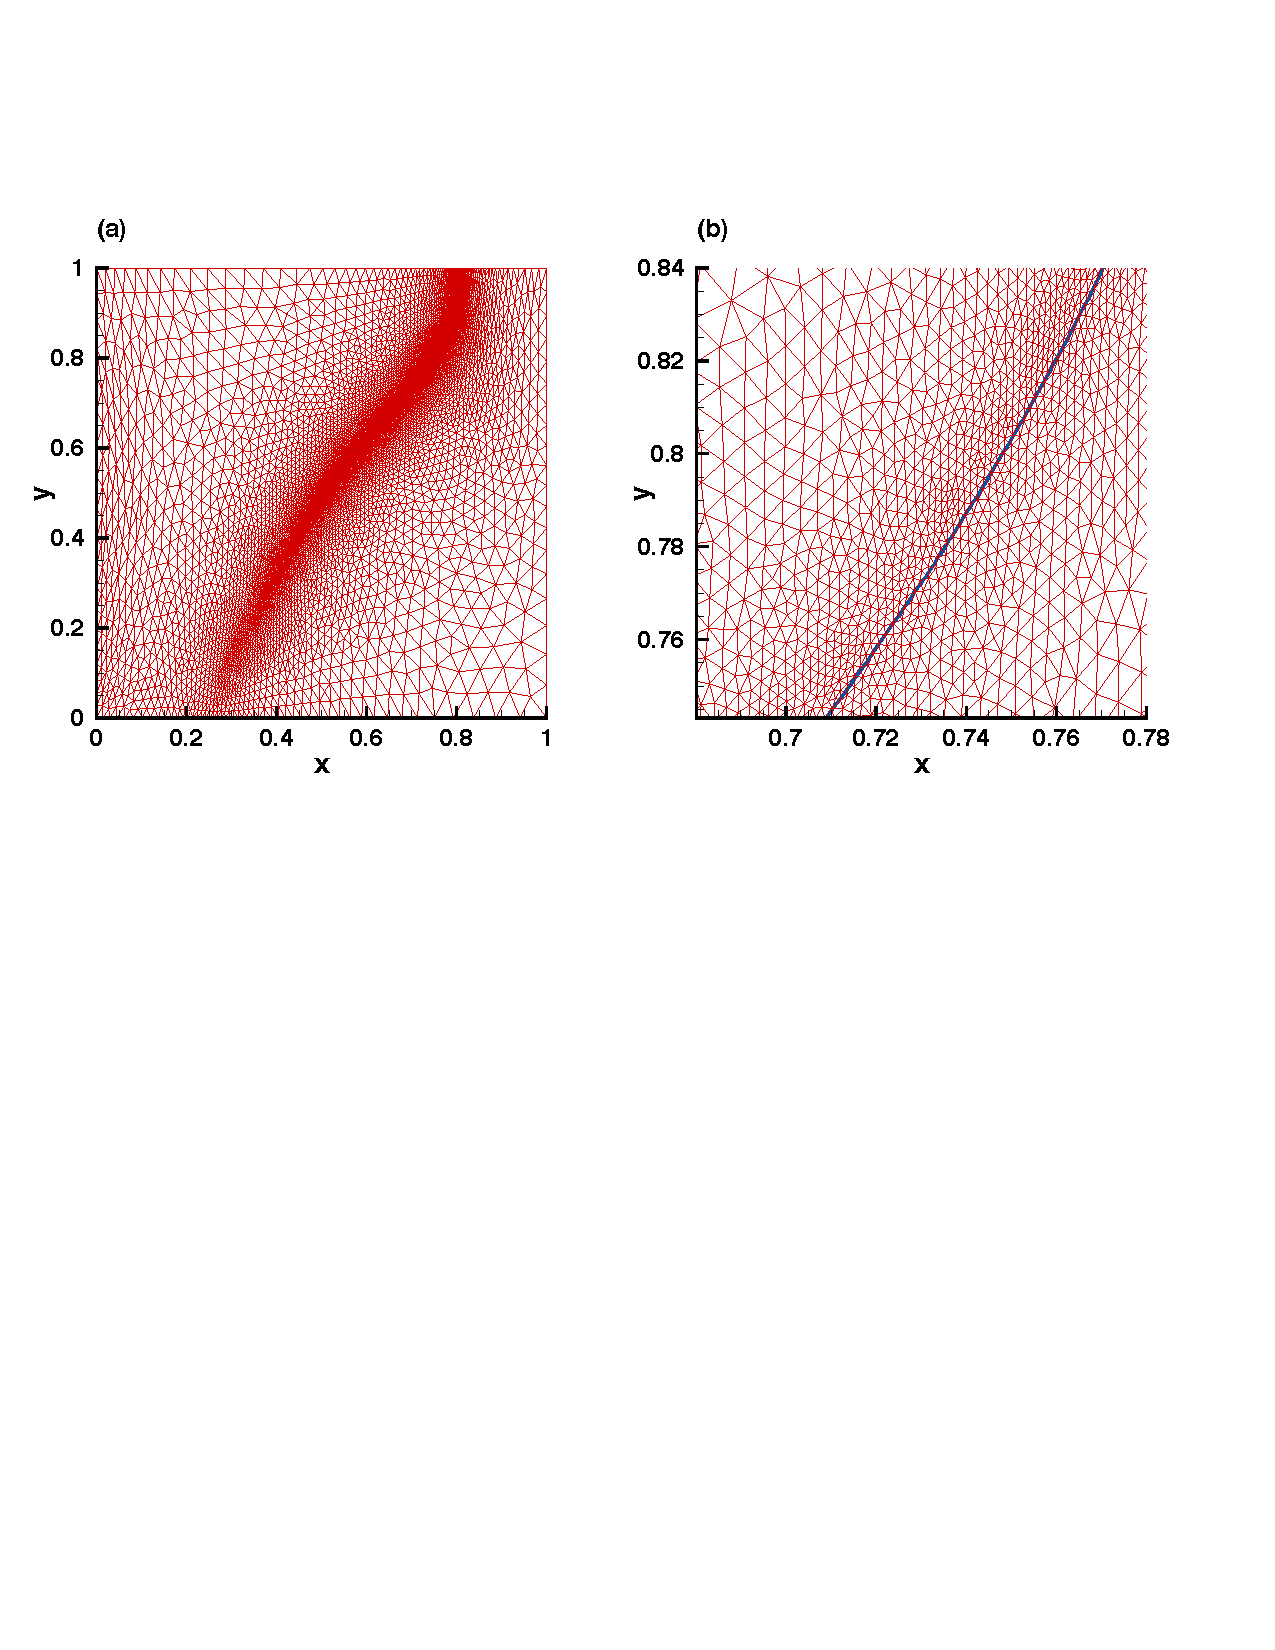
\includegraphics[width=\textwidth]{\figpath/Fig_cap_melting/Mesh_MELT}
	\end{center}
	\caption{Adapted mesh during PCM melting. (a) $4,211$ triangles: mesh is refined around the melting front $\theta=0$ and in the fluid where velocity gradients exists. (b) zoom showing the decrease of the mesh size around the temperature isoline $\theta = 0$.}
	\label{fig:pcm-mesh}
\end{figure}

%\begin{figure}
%	\begin{center}
%		\includegraphics[width=.95\textwidth]{\figpath/Fig_cap_melting/MESH_analysis_PCM}
%		\includegraphics[width=.95\textwidth]{\figpath/Fig_cap_melting/NU-LF_MESH_analysis_PCM}
%	\end{center}
%	\caption{Adapted mesh during PCM melting. (a) $2,870$ triangles: mesh is refined around the melting front $\theta=0$ and in the fluid where velocity gradients exists. (b) zoom showing the decrease of the mesh size around the temperature isoline $\theta = 0$.}
%	\label{fig:pcm-mesh}
%\end{figure}

Mesh adaptivity is performed at each time step and offers a refined discretization of the regularization region where sharp gradients have to be accurately captured.  
%To ensure that we obtain a grid-converged solution, we perform different mesh resolutions  for the case presented in Fig. \ref{fig:pcm-CK} and test the influence of the number of triangles on the melting front, the Nusselt number, and the liquid fraction.
Fig. \ref{fig:pcm-mesh} shows the adapted mesh during the melting of Gallium PCM in a square cavity.
The mesh is remarkably refined around the melting front (Fig \ref{fig:pcm-mesh}b), localized by the temperature $\theta = 0$, and in the fluid region around the convection cells, while coarser mesh is applied in the solid.
The typical number of triangles of the generated adaptive mesh, during the simulation is $4,000$ triangles. 
Non-adapted grids offering the same spatial resolution everywhere inside the computational domain would have resulted in $N_t=9.94 \cdot 10^{10}$ triangles. 
Consequently, mesh adaptivity greatly helps in reducing the computational time. 
The mesh adaptivity capability to capture several interfaces is the striking feature of our method, mainly its capability to track efficiently two solidification fronts during PCM solidification or the density inversion interface during the water freezing will be discussed in Sec. \ref{sec-water-freeze}.

\subsection{Initialization}
For the melting process, the PCM is initially solid and the temperature is set to a cold temperature $\theta_c$ under the temperature of fusion $\theta_f$.
However, increasing abruptly the boundary temperature to a hot temperature $\theta_h$, over the temperature of fusion, in order to initiate the melting process is numerically complicate because of the strong temperature gradient between the wall and the PCM.
A first usual approach consists of setting a very thin fluid layer of thickness $\delta x \sim 0.01$ with isothermal temperature in the vicinity of the hot wall (see \cite{dan-2014-JCP,Belhamadia2004_S}.
A second approach, based on an establishment regime, will be applied in the current work.
The temperature at the hot wall and the Rayleigh number are increased smoothly over a small time steps up to reaching the correct value of $\theta_h$ and $\Ray$.
This approach has physical significance and is more robust when higher Rayleigh number simulations are performed.
Concerning the solidification stage, mainly the water freezing case, a 'hot' and a 'cold' restarts are carried out.
The first consists of establishing a steady state regime by solving first the steady Eq. \eqref{eq-weak-steady} and dropping then smoothly the temperature of the cold wall under the temperature of fusion.
The second sets directly $\theta_c$ under the temperature of fusion besides the motionless fluid, inducing thus huge gradients near the wall, requiring very small triangles therein.

\newpage

\section{Melting of n-octadecane PCM in a square cavity} \label{sec: melting-2D} %: Comparison with experimental data of \cite{Okada1984}  and \cite{gong2015numerical}, and numerical data of \cite{bertrand1999melting}.}
We start the validation of our algorithm for phase-change systems by simulating the melting of n-octadecane PCM within differentially heated rectangular cavity.
Three cases are investigated: \\
-- \underline{\textit{Benchmark $\#1$}}: Experimental investigation by \cite{Okada1984} of the melting of n-octadecane PCM. \\ % in enclosures of height $H=1.5$ cm. \\
%The non-dimensional parameters resulting from the physical properties of n-octadecane presented in Tab. (\ref{tab-param-PCM}) are: $\Ray = 3.27 \cdot 10^5$, $\Prd = 56.2$ and $\Ste = 0.045$ .\\
-- \underline{\textit{Benchmark $\#2$}}: Experimental and numerical investigations by \cite{gong2015numerical} of the melting of PCM inside a transparent building brick. \\ % of height $H = 15.2$ cm. \\
%The non-dimensional parameters corresponding to their experimental study are: $\Ray = 2.48 \cdot 10^8$, $\Prd = 50$ and $\Ste = 0.072$.\\
-- \underline{\textit{Benchmark $\#3$}}: Numerical comparison of various numerical methods, presented by \cite{bertrand1999melting}. \\ % considering high value of the Rayleigh number. \\
%The computed parameters are: $\Ray = 10^8$, $\Prd = 50$ and $\Ste = 0.1$.\\
%
\begin{table}[!ht]
   \begin{center}
	\begin{tabular}{*{7}{c}}
  	 	&  & $\Ray$ & $\Prd$ & $\Ste$ & $\delta t$ & $V_{ref}$ \\
   		\bottomrule
   		\multirow{3}{*}{n-octadecane} & Bench $\#1$ &   $3.27 \cdot 10^5$ &  $56.2$ & $0.045$ & $10^{-1}$ & \multirow{3}{*}{$\frac{\nu_l}{H}$} \\
    		& Bench $\#2$ & $2.48 \cdot 10^8$ & $50$  & $0.072$ & $10^{-3}$ &  \\
    		& Bench $\#3$ & $10^8$ & $50$  & $0.1$ & $10^{-5}$ &  \\
    		\hline
  		 \multicolumn{2}{c}{Gallium}  & $7 \cdot 10^5$ &$0.0216$  & $0.046$ & $10^{-3}$ & $\frac{\nu_l}{H}$ \\
		 \bottomrule
      \end{tabular}
   \end{center}
   \caption{Dimensionless parameters for melting of n-octadecane PCM.}
   \label{tab-param-pcm}
\end{table}

\begin{figure}
	\begin{center}
		\includegraphics[width=.9\textwidth]{\figpath/Fig_cap_melting/MESH_analysis_PCM}
		\includegraphics[width=.9\textwidth]{\figpath/Fig_cap_melting/NU-LF_MESH_analysis_PCM}
	\end{center}
	\caption{{Benchmark $\#1$}. Influence of the mesh resolution on the numerical solution at  dimensionless time $t=78.7$. Mesh is refined around the melting front $\theta=0$ and in the fluid where velocity gradients exists. Solid lines denote the solid-liquid interface. Number of triangles: (a) $48,247$, (b) $21,093$, (c) $2,870$, (d) $820$. The location of the interface (e) and the time evolution of the Nusselt number (f) are compared.}
	\label{fig:mesh-convergence-OKADA}
\end{figure}

The experimental investigation of \cite{Okada1984} in \textit{Benchmark $\#1$} consists of a differentially heated square cavity of dimensions $1.5$ cm $\times \, 1.5$ cm.
The left and the right walls are isothermal and the top and the bottom walls are adiabatic.
No-slip boundary conditions are prescribed on the velocity over the whole $\partial \Omega$.
The physical parameters used in our simulations are given in Tab. \ref{tab-param-pcm}.

To ensure that we obtain a grid-converged solution, we first perform different mesh resolutions for \textit{Benchmark $\#1$} by keeping the minimum edge length constant and increasing {\em hmax} from $10^{-2}$ to $10^{-1}$.
A snapshot of the adapted mesh at $t=78.7$ is reported in Fig. \ref{fig:mesh-convergence-OKADA}.

\noindent -- {\em Mesh} $\# 1$ (Panel a): $N_t = 48,247$ triangles and $314,203$ degree of freedom (d.o.f), \\
-- {\em Mesh} $\# 2$ (Panel b): $N_t = 21,093$ triangles and $143,202$ d.o.f, \\
-- {\em Mesh} $\# 3$ (Panel c): $N_t = 2,870$ triangles and $318,974$ d.o.f, \\
-- {\em Mesh} $\# 4$ (Panel d): $N_t = 820$ triangles and $5,544$ d.o.f.
%ranging from $N_t = 1,000$ triangles to $N_t = 50,000$ triangles, and test the influence of the number of triangles on the melting front and the Nusselt number  for \textit{Benchmark $\#1$} case.
%A snapshot of the mesh resolution at $t=78.7$ is depicted in Panels (a) to (d) of Fig. \ref{fig:mesh-convergence-OKADA}.

\noindent For all performed mesh, one can observe %refined meshes along the interface and the heated wall where high gradients could be localized.
finer mesh at the boundary layer region due to the high velocity gradients, mainly near the walls, and along the interface $\theta=0$, while coarser mesh is applied in the solid region.
We note however that a ratio of $10$ is set for {\em hmax} between {\em Mesh} $\# 1$ and {\em Mesh} $\# 4$, resulting to a ratio of $50$ on the number of d.o.f. using quadratic discretization of $T$.
Simulations are performed using $\delta t = 10^{-2}$ to ensure small time discretization errors.
%Differences of order of $54.7$ could be observed between {\em Mesh} $\# 1$ and .
The location of the solid-liquid interface and the time evolution of the Nusselt number related to each of the four adapted meshes are compared in Panels (e) and (f). 
The maximum discrepancies for the location of the melting front occur at the top of the cavity since the highest velocity is reached in this region because of the clockwise recirculation of the flow. 
We compare thus the position of the solid-liquid interface along  $x$-direction at $y=1$.
The coarser grid ({\em Mesh} $\# 4$) exhibits the highest gap with respect to the most refined  {\em Mesh} $\# 1$, with a relative error of $2.14 \%$ for the location of the melting front at the top of the cavity and by overestimating the heat transfer of an order of $3.83 \%$.
For {\em Mesh} $\# 3$, in which the mesh resolution is increased by a ratio of $3$ compared to the coarse mesh, reasonable differences of $0.042 \%$ and $0.039 \%$ are noticed for both $\mathcal{N}\!u$ and the interface.
Finally, from {\em Mesh} $\# 2$, variations lower than $0.01 \%$ are recovered.
However, since a balance between the accuracy and the computational time is sought, the subsequent simulation are performed using parameters of {\em Mesh} $\# 3$, summarized in Tab. \ref{tab-param-mesh}.
Solutions using {\em Mesh} $\# 3$ were actually performed with only $2876.39$ CPU seconds, while $12$ CPU hours were needed for {\em Mesh} $\# 1$.
\begin{table}
   \begin{center}
      \begin{tabular}{*{5}{cl}}
               	hmin & hmax & adaptratio & errh & nbvx \\
         	\hline
         	$10^{-3}$ & $0.1$ & $1.5$ & $0.01$ & $50,000$ \\
      \end{tabular}
   \end{center}
   \caption{Mesh adaptivity parameters used for {\em Mesh} $\# 3$.}
   \label{tab-param-mesh}
\end{table}

\begin{figure}
	\begin{center}
		\includegraphics[width=0.9\textwidth]{\figpath/Fig_cap_melting/MELT_Okada_valid_2}
	\end{center}
	\caption{\textit{Benchmark $\#1$}. 
	(a) Temperature isoline at $t=78.8$.
	(b) Location of the interface. Comparison with experimental data of \cite{Okada1984} and numerical solutions of \cite{dan-2014-JCP} and \cite{Wang2010} for two time instants ($t=39.9$ and $78.8$).
	(c) Vertical component of velocity field and location of the interface at $t=78.8$.
	(d) Adapted mesh with $2,900$ triangles at $t=78.8$. 
	% Benchmark 1: 
	%(b) Comparison with both experiment and simulation of \cite{gong2015numerical} for five time instants  ($\tau = 0.0002$, $0.00050$, $0.00067$, $0.00125$, $0.00252$). Benchmark 2: $\Ray = 2.48 \cdot 10^8$, $\Pr = 50$ and $\Ste = 0.072$.
	}
	\label{fig:pcm-valid}
\end{figure}

We present in Fig. \ref{fig:pcm-valid} the computed solution for \textit{Benchmark $\#1$} case using {\em Mesh} $\# 3$.
Panel (a) displays the temperature distribution of the PCM at dimensionless time $t=78.7$ in the unit square domain $\Omega = (0,1)^2$. 
The enclosure is heated from the left and the melting PCM expands from the left to the right (the blue color denotes the solid region).
A non-planar shape of the phase-change interface could be observed due to effect of the natural convection in the liquid phase.
Further comprehensive descriptions of the influence of the liquid flow on the interface will be discussed in Chapter \ref{chap-MELTING-ANALYSIS}.
Panel (b) compares the location of the solid-liquid interface with experimental investigation of  \cite{Okada1984}.
For two particular time instants, $t=39.9$ and $t=78.7$, we could compare our results to available experimental \citep{Okada1984} and numerical \citep{Okada1984,Wang2010,dan-2014-JCP} data. 
In the experimental set up, the author has reported that the top of the PCM was not perfectly insulated and consequently the growth of the experimental upper melting front was delayed.
The current work agrees well with the experimental results of \cite{Okada1984} at the bottom part of the melting front.
However, our results overestimate the location of the front in the top part of the cavity, which could be related to the experimental heat loss mentioned by the author. 
Moreover, our results are qualitatively in a better agreement with experimental data than previously published numerical results. 
This is a direct consequence of the precise tracking of the melting front achieved by the mesh adaptivity performed at each time step.
\cite{Wang2010} have used a FV code with a fixed mesh of resolution $[60 \times 60]$, and \cite{dan-2014-JCP} have used a first order FE method with adaptive grid. 

%\noindent The vertical component of the velocity field and the resulted adapted mesh at $t=78.7$ are given in panels (c) and (d).
%Thinner mesh could be observed in the boundary layer region due to the high velocity gradients, mainly near the walls, and along the interface $\theta=0$, while coarser mesh is applied in the solid region.
%Panel (c) corresponds to adapted mesh with $2,900$ triangles. 
%The numerical solution presented in Fig. \ref{fig:pcm-valid} were obtained with only $2876.39$ CPU seconds.

Numerical results for \textit{Benchmark $\#2$} are depicted in Fig. \ref{fig:pcm-Gong}.
The numerical simulation is performed using $\delta t = 10^{-3}$ and a total runtime of $19,231$ CPU seconds using $4,198$ triangles.
\cite{gong2015numerical} have investigated the melting of octadecane PCM inside a transparent building brick of dimensions $15.2$ cm $\times$ $3$ cm.
Panel (a) illustrates the temperature distribution in the melting PCM, the streamlines, and the phase-change interface obtained by the present finite element simulation.
Panel (b) compares the location of the melting front for five particular time instants: $t=0.153$, $0.347$, $0.465$, $0.869$, and $1.759$, with numerical and experimental data by \cite{gong2015numerical}.
Their numerical simulations were based on the thermal lattice Boltzmann method (TLBM), in which the natural convection got solved by LBM and the temperature equation was solved by finite difference scheme using enthalpy method. 
The difficulty here compared to the first validation case is the presence of a stronger natural convection flow in the fluid due to the higher value of the Rayleigh number.
%The location of the melting front is compared for five particular time instants: $\tau = 0.0002$, $0.00050$, $0.00067$, $0.00125$ and $0.00252$.
%Their numerical simulation has been performed using a hybrid thermal Lattice Boltzmann method combined with an enthalpy method. 
%The location of the interface is compared for five particular time instants: $\tau = 0.0002$, $0.00050$, $0.00067$, $0.00125$ and $0.00252$.
We notice a very good agreement with respect to both numerical and experimental data of \cite{gong2015numerical}.

\begin{figure}
	\begin{center}
		\includegraphics[width=0.95\textwidth]{\figpath/Fig_cap_melting/MELT_Gong_valid}
	\end{center}
	\caption{\textit{Benchmark $\#2$}. 
	(a) Temperature distribution, streamlines, and solid-liquid interface at dimensionless time $t=1.759$.
	(b) Comparison of the location of the solid-liquid interfaces, with both experiment and simulation of \cite{gong2015numerical}, for five time instants  ($t=0.153$, $0.347$, $0.465$, $0.869$, and $1.759$).}
	\label{fig:pcm-Gong}
\end{figure}

A last validation case, for the n-octadecane PCM, is also investigated to test the robustness of the method.
\cite{bertrand1999melting} compiled results provided by five different authors (Lacroix, Le Qu{\'e}r{\'e}, Gobin-Vieira, Delannoy and Binnet-Lacroix). Results provided by these authors will be hereafter referred to as (say) 'Lacroix, from \cite{bertrand1999melting}'.
They have attempted a first comparison by taking several numerical methods to compute the basic configuration presented in this section. 
Two investigators among the five failed to predict the process and showed unrealistic behaviors (see Figs. \ref{fig Bertran} and \ref{fig-Nu-Lf-Bertran}):
Lacroix and Delannoy seem to be insufficiently converged (Fig. \ref{fig Bertran}), and Binet-Lacroix overestimates the average Nusselt number by more than $30 \%$ (Fig. \ref{fig-Nu-Lf-Bertran}).
Hence, this collection of results allows us to compare our numerical method and check whether or not realistic results are obtained for complex physical configurations.

\noindent We further inspect the melting front, the temporal evolution of the liquid fraction $L_f$ and the Nusselt number $\mathcal{N}\!u$ at the left wall ($x=0$), for each of the five methods presented by \cite{bertrand1999melting}.
For the liquid fraction, the initial solid state corresponds to $L_f = 0$, while  $L_f = 1$ indicates the  complete melting of the PCM. 
%The average Nusselt number $N\!u$ at $x=0$ left boundary is defined as follows:
%\begin{equation}\label{eq-Nu}
%N\!u = \int_{0}^1 \left(\frac{\partial \theta}{\partial x}\right)_{x=0}\, dy.
%\end{equation}
%\\
\begin{figure}
	\begin{center}
		\begin{minipage}[t]{0.8\textwidth}
			\includegraphics[width=\textwidth]{\figpath/Fig_cap_melting/fig03}
		\end{minipage}
	\end{center}
	\caption{\textit{Benchmark $\#3$}. Location of the solid-liquid interface at dimensionless time (panels a to d) $t=0.25$,  $t=1$, $t=3$, and $t=5$, compared with five simulations presented by \cite{bertrand1999melting}. 
	} \label{fig Bertran}
\end{figure}
\begin{figure}
	\begin{center}
		\begin{minipage}[t]{0.8\textwidth}
			\includegraphics[width=\textwidth]{\figpath/Fig_cap_melting/Lf-Nu_Bertrand}
		\end{minipage}
	\end{center}
	\caption{\textit{Benchmark $\#3$}: $\Ray = 2 \cdot 10^8$, $\Prd = 50$ and $\Ste = 0.1$. Time evolution of the liquid fraction (a) and  the  Nusselt number (b) compared with five simulations presented by \cite{bertrand1999melting}.
	} \label{fig-Nu-Lf-Bertran}
\end{figure}
The phase-change interface for four time steps, $t=0.25$,  $t=1$, $t=3$ and $t=5$ is represented in Fig. \ref{fig Bertran}.
Our results are for each case in fairly good agreement with those of Gobin and those of  Le Qu{\'e}r{\'e}.
Gobin uses a front-tracking method using a coordinate transformation with a finite volume method with a $62 \times 42$ grids.
Le Qu�r� solves a single domain model using a second order scheme with a finite volume method with a $192 \times 192$ grids  (\cite{gobin2000melting}).
The time evolution of the liquid fraction and the  Nusselt number are moreover plotted in Fig. \ref{fig-Nu-Lf-Bertran}.
A very good agreement is obtained with Gobin and Le Qu{\'e}r{\'e}.
A relative difference, less than $2\%$ is noticed for the Nusselt number, and a dispersion, smaller than $4 \%$, for the melted fraction.
The high value of the Rayleigh number, $\Ray = 10^8$, results in a very demanding numerical test.
The high velocity, inducing a very narrow thermal boundary layer can lead to unrealistic results and some numerical methods have failed.
The interest of the mesh adaptation is clearly evidenced since a typical number of triangles of $N_t = 7,000$ were used during the simulation, which have necessitated $40,522$ CPU seconds of run.


\section{Melting of Gallium in a rectangular cavity} \label{sec-melt-gallium}

%The observation on the melting of the gallium in a rectangular cavity was a controversy since the question if  the flow in the fluid is monocellular of multicellular was raised by \cite{dantzig1989modelling}.
The melting of tin or Gallium in a rectangular cavity, which corresponds to low-Prandtl fluids, was a controversial case since  \cite{dantzig1989modelling} raised the question 
whether  the convection in the fluid is mono-cellular or multi-cellular.
The experimental result exhibits indeed a mono-cellular structure, while many researchers claim this observation to be incorrect.
Prior to \cite{dantzig1989modelling} note, both experimental and numerical results support a single cell solution in the fluid phase.
Later, simulations provide solutions with multicellular flow. 
During the comparison exercise investigated by \cite{bertrand1999melting}, Le Qu�r� and Couturier-Sadat have predicted a different shape of the front corresponding the low-Prandtl simulation, induced by the multi-cellular structures of the flow in the melted PCM.
\cite{le1999note} have shown that the multi-cellular structures result from thy hydrodynamic instabilities during the conduction regime before the onset of convection.
Moreover, numerical investigation of \cite{hannoun2003resolving}, testing the influence of the mesh resolution and the numerical method's order, indicates clearly that mono-cellular observation is caused by a problem of convergence of the numerical solution. It can be due to the grid size or inconsistencies in the mathematical model.

\noindent Therefore, this test case simulating the melting of Gallium is a relevant exercice to test the consistency of our method.
To capture the very small cell during the first step of the melting, \cite{hannoun2003resolving} uses a $800 \times 1,120$ fixed grids in a rectangular domain of dimensions $6.35$ cm $\times \, 8.89$ cm. 
The authors have reported that the melting solution up to 32 s have required about $980$ CPU hours on a Compaq Alpha ($667$ MHz, ev$67$) processor.
However, a maximum of $4, 820$ triangles are necessary with our adaptive method, and only $4$ CPU hours are spent to reproduce the numerical result of \cite{hannoun2003resolving} up to the final time 280s, on an Intel ($2,8$ GHz, Core i$7$) processor.

\begin{figure}
	\begin{center}
		\begin{minipage}[t]{\textwidth}
			\includegraphics[width=.9\textwidth]{\figpath/Fig_cap_melting/figsCPC_11}
			\includegraphics[width=.9\textwidth]{\figpath/Fig_cap_melting/HANNOUN_mesh_Nu}
		\end{minipage}
	\end{center}
	\caption{Melting of Gallium: temperature field, streamlines, and melting front for dimensionless time instants (panels a to d): 
	$t = 0.0015$, $0.006$, $0.01$, and $0.019$. Adapted mesh corresponding to $t = 0.019$ (e). Time evolution of the Nusselt number (f). For a better view of the convection cells, a ratio $2:1$ was used for the axis dimensions.} \label{fig-Gallium}
\end{figure}

The time evolution of the flow  is presented in the Fig. \ref{fig-Gallium}. 
The enclosure is heated from the left (vertical) wall and the horizontal walls are adiabatic and no-slip.
The physical properties of the Gallium and the dimensionless parameters of the run are given in Tabs. \ref{tab-param-PCM} and \ref{tab-param-pcm}.
Temperature field, streamlines and position of the melting front are displayed for several time instants: $t= 0.0015$, $0.006$, $0.01$, and $0.019$.
These values were chosen to visualize the merging of convection cells in the fluid flow and correspond to physical times $20s, 85s, 155s, 280s$ in \cite{hannoun2003resolving}.
The number of rolls was considered as a validation criterion by several authors 
\citep{hannoun2003resolving,cerimele2002numerical,giangi2000melting}.
Three cells are observed  at $t=0.006$ (Fig. \ref{fig-Gallium}). The number of cells decreases later through a process of roll merging, as it was also reported  by \cite{le1999note} and \cite{hannoun2003resolving}. Our numerical results are in good agreement with the observations of \cite{hannoun2003resolving}, \cite{cerimele2002numerical} and \cite{giangi2000melting}.
The adapted mesh corresponding to $t = 0.019$ is illustrated in Panel (e).
The mesh is well refined along the isoline $\theta = 0$ denoting the interface, and around the convective cells.

The time evolution of the Nusselt number at the heated vertical wall is plotted in Fig. \ref{fig-Gallium}f.
One can note that the quasi-steady evolution of $\mathcal{N}\!u$ in Fig. \ref{fig-Nu-Lf-Bertran}, for high-Prandtl fluid simulations, is not recovered. 
This is in total accordance with the instability analysis of \cite{le1999note} showing that the Nusselt number becomes unsteady starting from a critical time, for Rayleigh numbers greater than $10^5$ for low-Prandtl simulation, 
while no instability could be found whatever the value of $\Ray$ for high-$\Prd$ cases.
The first slight oscillation at the very earlier time steps corresponds to the onset of the convective flow induced by the first instability of the conductive regime,
which is followed by a nearly constant evolution of $\mathcal{N}\!u$ from $t = 0.01$ to $t = 0.02$ during the cell-merging processes.
High oscillations of the heat transfer are then observed, which is feature of the onset of the second oscillatory instability.
A zoom of the periodic evolution of the Nusselt number is displayed in Panel (f).
Finally, the amount of heat transfer decreases from $t=0.13$ when the front reaches the cold (right) vertical wall.

\section{Melting of cylindrical PCM with inner heated tubes} \label{subsec-luo}
Cases presented in Secs. \ref{sec-melt-gallium} and \ref{sec: melting-2D} considered phase change problems evolving in a simple geometry, a rectangular box.
%We have simulated previously phase-change problems within rectangular cavities.
%A more complex system is studied in this section, by simulating the melting of pure PCM on multitube thermal energy storage systems.
A more complex geometry, suggested by \cite{luo2015lattice}, is simulated in this section. It consists of a cylindrical PCM of  radius $R=1$ with tube inclusions of different arrangements.
%Similar configurations were studied by \cite{luo2015lattice}. Hence we could compare our numerical results to those of \cite{luo2015lattice}.
%The interest is twofold: the geometry is challenging since is it complex and \cite{luo2015lattice} uses Lattice Boltzmann method, a microscopic model, which is different from previous validation cases.
The interest in studying this case is not solely the challenge of the complex configuration, but also the possibility to compare our results with those of \cite{luo2015lattice}, obtained using a completely different model based on the Lattice Boltzmann Method. This configuration is also interesting from a practical point of view.
\cite{agyenim2010review} pointed out that more than $70\%$ of the PCM containers used for heat storage  are using shell-tube systems.

%Cylindrical PCM of dimensionless radius $R=1$ with tube inclusions are studied.
%Shell and tube PCM are indeed most intensely used in latent heat energy storage systems.
%\cite{agyenim2010review} pointed out, in a critical review of materials used for heat storage, that more than $70\%$ of the PCM container are using the shell and the tube system.

We simulate three cases taking into account one heated tube, four heated tubes, and nine heated tubes with the same contact area.
For the one heated tube case, the radius $R_i$ of the inner tube is one-quarter of the outer tube ($R_i = R/4$), for four heated tubes $R_i = R/8$ and for nine heated tubes $R_i = R/12$.
A Dirichlet boundary condition is applied to inner tubes $\theta = \theta_h$,
and a Neumann boundary condition $\frac{\partial \theta}{\partial n} = 0 $ is used at the outers.
Homogenous Dirichlet boundary conditions ($\vec u = 0$) are prescribed on the velocity throughout on $\partial \Omega$.
The physical parameters of the simulation are:  $\Ray = 5 \cdot 10^4$, $\Prd =0.2$ and $\Ste = 0.02$.
It is worth noting that only the half of the domain is simulated since the problem is axisymmetric for the investigated $\Ray$ number.
At $t=0$, the PCM is completely solid with isothermal temperature $\theta_0$ lower than the temperature of fusion.
Immediately after the pipe placed on the center of the enclosure is heated, the melt layer expands in the radial direction.
The mesh is refined initially around inner tubes, and is dynamically adapted at each time step around the melting front and the thermal boundary layer area.

Fig. \ref{fig-Luo-Field} shows  the temperature field and the position of the solid-liquid interface (black line) related to the three configurations for time instants corresponding to the same liquid fraction $L_f=80\%$. 
The distribution of  the inner tubes in the liquid phase influences directly the fluid motion and the shape of melting front.
The more the number of inner tubes, the stronger the natural convection is  in the melted PCM. 
The shape of the solid-liquid interface displays complex patterns, depending on the space arrangement of the inner tubes. 
This is linked to the effect of the fluid motion in the presence of obstacles as it was also noticed in Sec. \ref{sec: natconv-water}.
The mesh is nicely adapted following the evolution of the melting interface, even after its separation in several distinct fronts touching the outer boundary (see Figs. \ref{fig-Luo-Field}b, c). 

To estimate the efficiency of each configuration, we plot in Fig. \ref{fig-Lf-Luo} the time evolution of the liquid fraction $L_f$. 
By including more heated tubes the heat transfer is enhanced, inducing a faster melting time.  
The nine-tube configurations melts $5$ times faster than the reference configuration with one tube.
A reasonably close match with numerical results of \cite{luo2015lattice} is confirmed by looking at Fig. \ref{fig-Lf-Luo}a.
We also assess the effect of tubes arrangements with fixe obstacle number. 
Three arrangements are simulated with $9$ obstacles and reported in Fig. \ref{fig-Lf-Luo}b: centrosymmetric, inline, and staggered arrangements.
Centrosymmetric arrangement appears to provide a better heat transfer compared to the others.
The inline and the staggered arrangements exhibit similar trends, with a slightly faster melting rate within the inline arrangement.
The difference is explained by \cite{luo2015lattice} by the contribution of conductive heat transfer induced by the arrangements.

\begin{figure}
	\begin{center}
		\begin{minipage}[t]{\textwidth}
			\includegraphics[width=.9\textwidth]{\figpath/Fig_cap_melting/figsCPC_09}
		\end{minipage}
	\end{center}
	\caption{Temperature fields for the melting of a cylindrical PCM with inner heated tubes. 
	Time instants corresponding to the same liquid fraction $L_f=80\%$. 
	Configurations with  (a) one tube ($t=2.5$), (b) four tunes ($t=0.99$) and (c) nine tubes ($t=0.4$).
	Melting  front are localized with black lines (only half of the domain is simulated).  
	}  \label{fig-Luo-Field}
\end{figure}

\begin{figure} 
	\begin{center} 
		\begin{minipage}[t]{\textwidth}
			\includegraphics[width=.9\textwidth]{\figpath/Fig_cap_melting/Lf_Luo_3}
		\end{minipage}
	\end{center}
	\caption{Time evolution of the liquid fraction for one, four, and nine heated tubes. (a) Comparison with numerical results of \cite{luo2015lattice} (b) comparison of centrosymmetric, inline, and staggered arrangements.} \label{fig-Lf-Luo}
\end{figure}

\newpage
\section{Solid crust formation in a highly distorted mesh} \label{sec-solid-crust}
%
%\begin{figure} 
%	\begin{center}
%		\begin{minipage}[t]{\textwidth}
%			\includegraphics[width=\textwidth]{\figpath/Fig_cap_melting/DOMAIN_Nourgaliev}
%		\end{minipage}
%	\end{center}
%	\caption{Highly distorted computational domain for solid crust formation by \cite{nourgaliev2016fully}.}  \label{fig-Domain-Nourgaliev}
%\end{figure}

The solid crust formation inside a highly distorted domain, simulated by \cite{nourgaliev2016fully} is of interest in this section.
Our emphasis here is placed on the ability of our method to tackle also solidification problem, especially in irregular domain (see Fig. \ref{fig-Nourgaliev}).
%For this purpose, we use the computational domain shown in Fig. (\ref{fig-Domain-Nourgaliev}) to simulate the solidification of liquid PCM at steady its steady state.
%The six geometrical parameters, $X_0, X_1, Y_0, Y1, \alpha, \beta$ are set as follow:
%\begin{eqnarray}
%	X_0 &=& -1, \\
%	X_1 &=& 1, \\
%	Y_0 &=& -0.5, \\
%	Y_1 &=& 0.5, \\
%	\alpha &=& \beta = 20^o,
%\end{eqnarray}
%where $\alpha$ and $\beta$ define the level of stretching and distortion.

The fluid is initially motionless with an initial dimensionless temperature $\theta_0 = 2$ well above the temperature of fusion.
The temperature of fusion is set to $\theta_f = 1.4$ according to \cite{nourgaliev2016fully} parameters.
It is worth noting that \cite{nourgaliev2016fully} have used $T_{ref} \ne T_f$ thus $\theta_f \ne 0$.
The left side is set at cold temperature $\theta_c = 1.39$ in the initial stage as the right wall was kept constant at a hot temperature $\theta_h = 2$, so that a steady-state natural circulation should be established. 
The cold temperature at the left wall is then dropped smoothly down to $\theta_c = 1$, below the temperature of solidification, starting the formation of a solid crust layer. 
The top and the bottom walls are adiabatics.

The dimensionless parameters of the simulation are: $\Ray = 1 \cdot 10^6$, $\Prd =0.1$ and $\Ste = 4.854$.
%These investigated dimensionless parameters also allow to test the method's performance for low-Prandtl problem with high $\Ray$ and $\Ste$ numbers.
The scaling in Eq. \eqref{eq-scaling-3}, which is also used by \cite{nourgaliev2016fully}, is used in the current simulation.

\begin{figure}
	\begin{center}
		\begin{minipage}[t]{\textwidth}
			\includegraphics[width=\textwidth]{\figpath/Fig_cap_melting/figsCPC_12}
		\end{minipage}
	\end{center}
	\caption{Solid crust formation in a distorted mesh. Temperature field and streamlines of our simulation (a) and \cite{nourgaliev2016fully}  (b). } \label{fig-Nourgaliev}
\end{figure}

The temperature distribution, the streamlines as well as the melting front position are reported in Fig. \ref{fig-Nourgaliev}a and compared with the numerical results of \cite{nourgaliev2016fully},
who have used a second-order discontinuous Galerkin finite element method and a $\mu$-based technique to bring the velocity to zero in the solid region.
We are qualitatively in a fairly good agreement with \cite{nourgaliev2016fully}.
As expected, the high $\Ray$ and $\Ste$ dimensionless numbers combined with the distorted domain generate a complex vortical flow pattern in the melted PCM.
\cite{nourgaliev2016fully} have investigated a mesh convergence analysis and have concluded that a $512 \times 256$ mesh resolution is needed to get a full resolution of the five vortical structures in Fig. \ref{fig-Nourgaliev}b,
while only $2,769$ triangles are performed in the present simulation.
This case illustrates again the power of our mesh adaptivity algorithm.

%A last assessment of the performance of our sequential code is achieved in the next section by simulating the challenging case of water freezing.


\section{Water freezing} \label{sec-water-freeze}

We consider finally the difficult case of water freezing in a square cavity. 
After achieving the convection steady pattern in the cavity (see Fig. \ref{fig-T1w-isoT}), freezing starts by dropping progressively the temperature of the cold (right) wall from $T_c=\celsm{0}$ to  $T_c=\celsm{-10}$. 
%The new boundary condition on the right cold wall is imposed by setting a very thin layer of $\delta x=0.01$ with constant temperature $\theta=\theta_c$ and zero velocity.
The dimensionless parameters describing the problem are: $\Ray=2.518084 \cdot 10^{6}$, $\Prd=6.99$ and $\Ste = 0.125$.

Besides the complex fluid flow and the non-linear time evolution of the solid-liquid interface, the code have to handle the non-linear variation of the density presented in Eq. \eqref{eq-dens-nonlin}.
Moreover, one can note that in addition to the non-linear formulation of $f_B(\theta)$ in Eq. \eqref{eq-fBnonlin}, the coefficient $\Ray \times 1/(\beta \delta T)$ is very large since the Boussinesq approximation imposes a value of $\beta \delta T \ll 1$.
Since the assumption of constant conductivity is not accurate in the frame of water phase-change, $K(\theta)$ is regularized following the smooth function
\begin{equation}
K(T) =  1+ \frac{1}{2} \left( \frac{k_s}{k_l} - 1 \right)  \left\{
1 + \tanh \left( \frac{T_f-T}{R_{k}}\right)
\right\},
\label{eq-K-water}
\end{equation} 

\noindent with $k_s = 2.26$ and $k_l = 0.578$ the thermal conductivity of pure water in the solid and the liquid and $R_k = 0.0075$. 
%The mushy-zone definition is also slightly modified compared to the melting case.
We also define $\varepsilon_1 = 0$ and $\varepsilon_2 = 0.0075$, to ensure a very thin thickness of the mushy zone (see also \cite{dan-2014-JCP}).

Fig. \ref{fig-T2w-manip}a superimposes the experimental image from \cite{Kowalewski-1999} with our numerical results for the same physical time $t_{\varphi}=2340 [s]$. 
The flow pattern in the liquid phase also corresponds very well qualitatively to the experimental image. 
Since a good agreement with the experiment was sought,  the simulation was performed with very small time steps ($\delta t =10^{-5} \approx 0.014 [s]$), but still reasonable grids ($2,500$ triangles) due to the efficiency of the adaptivity algorithm.
The discrepancy between the experimental interface and the current simulation comes principally from the model, mainly the three-dimensional effects, the supercooling of water and realistic boundary conditions (see \cite{Giangi-2000,Kowalewski-1999,Kowalewski-2003}) that are not taken into account by the present numerical method.

The source term $S(\theta)$ is added to the metrics calculation presented in Sec. \ref{sec: natconv-water} to track the solidification front.
The mesh is thus refined along the line $\theta_m$ through the function $\Phi(\theta)$ defined in Eq. \eqref{eq-Stm}, the solid-liquid interface defined by $\theta = 0$ and in the boundary layer regions.
We use also both $\Phi(\theta^n)$ and $\Phi(\theta^{n+1})$ and $S(\theta^n)$ and $S(\theta^{n+1})$ in the adaptivity procedure.
The final mesh is displayed in Fig. \ref{fig-T2w-manip}c, clearly showing that the mesh is refined along the line $\theta=\theta_m$ and the solid-liquid interface ($\theta=0$). This allows to accurately capture the structure and the extent of the two recirculating zones, features that are difficult to obtain with fixed meshes (see discrepancies described in \cite{Giangi-2000,Kowalewski-1999,Kowalewski-2003}).
%As a consequence, the temperature level lines in Fig. \ref{fig-T2w-manip}d are smooth and clearly define the two interfaces in the system: the liquid-solid interface ($\theta=0$) and the density inversion interface ($\theta=0.4$) separating the two recirculating liquid regions.

The time evolution of the solid-liquid interface is depicted in Fig. \ref{fig-T2w-manip}d for several time instants from $t=0.05$ ($t_{\varphi}=70 [s]$) to final time $t=1.61$ ($2340 [s]$).
We observe first a straight shape of the front from $t = 0$ to $t = 0.05$.
Then, the top and the bottom of the freezing front move at different rates from $t = 0.3$ due to the competing effects of positive and negative buoyancy force in the unsolidified water.
The upper clockwise circulation has indeed the task to transport the hot liquid to the top wall and back along the extremum of the density variation (localized at the temperature isoline $\theta = \theta_m$), and slow consequently the growth of the solid layer.
However, the abnormal recirculation traps the cold liquid water at the bottom part of the cavity, enhancing thus the solidification rate at this region as one can note in Fig. \ref{fig-T2w-manip}d.

\begin{figure}
	\begin{center}
		%\includegraphics[width=\textwidth]{\figpath/Fig_cap_melting/figsCPC_15}
		\includegraphics[width=\textwidth]{\figpath/Fig_cap_melting/WFREEZ_thesis}
	\end{center}
	\caption{Freezing of pure water.  Configuration at (physical time) $t_{\varphi}=2340 [s]$ (t = 1.61): (a) experimental image from \cite{Kowalewski-1999}; the thick red line represents the solid-liquid interface computed with the present method (b) computed streamlines showing the two recirculating zones in the fluid phase.
	(c) finite-element mesh refined along the solid-liquid interface ($T = 0^oC$) and also along the line of maximum water density ($T = 4^oC$) (d) location of the solidification front for several time instants: from $t=0.05$ (corresponding to physical time $t_{\varphi}=70 [s]$) to $t=1.61$ ($2340 [s]$)}
	\label{fig-T2w-manip}
\end{figure}
%\begin{figure}
%	\begin{center}
%		\includegraphics[width=\textwidth]{\figpath/Fig_cap_melting/danaila_fig_11.jpg}
%	\end{center}
%	\caption{Freezing of pure water.  Computed configuration at (physical time)  $t_{\varphi}=2340 [s]$: (a) finite-element mesh refined along the solid-liquid interface ($T=\celsm{0}$) and also along the line of maximum water density ($T=\celsm{4}$)  (b) temperature iso-lines.}
%	\label{fig-T2w-manipT}
%\end{figure}

%\newpage
%\clearpage
\section{Concluding remarks}
In this chapter, we have demonstrated our numerical method's capability to produce highly accurate solutions of difficult multiphysics problems on several geometrical configuration.
The scope of complexity involve non-linear time evolution of the solid-liquid interface that could be highly deformed by the strong convection flow in the fluid phase.
Linear and non-linear expressions of the buoyancy force were investigated.

\noindent For the linear form of $f_B$, melting of pure paraffin (n-octadecane) and metal (Gallium) have been simulated in rectangular cavity heated from the side.
The choice of these materials is motivated by their physical properties relatively equal in both solid and liquid phases, the existence of many numerical and experimental investigations in the literature, and also the differences between the time evolution of the heat transfer for high and low $\Prd$ simulations.
Comparison with existing benchmarks have shown for each cases very good agreement.
The unsteadiness of the flow for the Gallium was observed in our simulations by the multi-cellular structure of the liquid flow and the high oscillating value of the Nusselt number.
The performance of the sequential code was also proven by simulating complex geometrical configuration.
The melting of cylindrical PCM including inner heated pipes and the solidification of liquid PCM inside irregular cavity have shown good agreement with existing numerical data.

\begin{table}
\centering
\begin{tabular}{*{4}{c}}
   \multicolumn{2}{c}{Case}  & {\small CPU time (s)} & {\small Number of triangles}  \\
  \toprule 
  \multirow{3}{*}{N-octadecane} & Bench $\#1$ & $2876.39$ & $2,900$ \\
  %\cline{2-4}
   & Bench $\#2$  & $19231$ & $4,198$ \\
   & Bench $\#3$  & $40522.7$ & $7,000$ \\
   \hline
   \multicolumn{2}{c}{Gallium} & $14621.2$ & $4,820$ \\
   \hline
  %\multicolumn{2}{c}{Cylindrical PCM} & $14621.2$ & $4,820$ \\
  \multicolumn{2}{c}{Cylindrical PCM} & $2060.42$ & $3,076$ \\
  \hline
  \multicolumn{2}{c}{Highly distorted PCM} & $6657.58$ & $2,769$ \\
%  {\small CPU time} & $2876.39$ & $40522.7$ & $2060.42$ & $14621.2$ & $6657.58$\\
%  {\small Number of triangles} & $2,900$ & $7,000$ & $3,076$ & $4,820$ & $2,769$ \\
\bottomrule
 \end{tabular}
\caption{Summary of melting simulations: number of triangles and CPU times.}
\label{tab-melt-cases}
\end{table}

\noindent The total CPU time and the typical number of triangles corresponding to each PCM cases are summarized in Tab. \ref{tab-melt-cases}.
Noticeable is the fact that, less than $2$ CPU hours are necessary for most of the simulations, even a sequential algorithm is used. 
The interest and the power of mesh adaptivity was highlighted by the simulation of the melting of the Gallium, since only $4$ CPU hours are necessary to perform this case, while $980$ CPU hours were needed by \cite{hannoun2003resolving} using fixed-grid algorithm.

\noindent Non-linear expression of $f_B$ was considered for the solidification of pure water case. 
Besides the high $\Ray$ and $\Ste$ considered in our simulations, the efficiency of the mesh adaptivity was demonstrated by its capability to track simultaneously the interface $\theta = \theta_f$ and the line $\theta = \theta_m$ separating the two recirculating liquid regions.
Qualitative comparison with experimental image exhibits good agreement.
The vortical structures in the liquid water were accurately captured and the density inversion interface was precisely solved.

\noindent More comprehensive description of the melting process will be presented in the next chapter.
Numerical and analytical tools will be performed to analyse and compare the melting of PCM heated either from the side or from below.

%%%%%%%%%%%%%%%%%%don't forget if needed %%%%%%%%%%%%%%%%%%%%%
%\section[toc version]{title version%
%              \sectionmark{head version}}
%\sectionmark{head version}
%%%%%%%%%%%%%%%%%%%%%%%%%%%%%%%%%%%%%%%%%%%%%%%%%%%%%%%%%%%%%%
\def\titcourt{Numerical comparison of basal and lateral melting of phase change materials}
\def\titlong{Numerical comparison of basal and lateral melting of phase change materials}
%%%%%%%%%%%%%%%%%%%%%%%%%%%%%%%%%%%%%%%%%%%%%%%%%%%%%%%%%%%%%%%%
\chapter[\titlong]{\titlong%
              \chaptermark{\titcourt}}
\chaptermark{\titcourt}
\label{chap-MELTING-ANALYSIS}
%%%%%%%%%%%%%%%%%%%%%%%%%%%%%%%%%%%%%%%%%%%%%%%%%%%%%%%%%%%%%%%%
%%%%%%%%%%%%%%%%%%%%%%%%%%%%%%%%%%%%%%%%%%%%%%%%%%%%%%%%%%%%%%%%
\begin{figure}
	\begin{center}
		\includegraphics[width=.9\textwidth]{\figpath/Fig_cap_melting_basal/Scheme-melt-lat} \\
		\includegraphics[width=.9\textwidth]{\figpath/Fig_cap_melting_basal/Scheme-melt-basal}
	\end{center}
	\caption{Sketch of the computational domain, boundary conditions for lateral (top) and basal (bottom) melting, streamlines showing the dynamic of the convection flow in the liquid phase (panels b and d) and solid-liquid interfaces (solid red lines).} \label{fig:melt-scheme}
\end{figure}
We have performed extensive validation of our numerical method in Chapters \ref{chap-NATCONV} and \ref{chap-MELTING}.
Very good agreement were noticed for each validation cases against well-known benchmarks and the robustness of the algorithm was proven by simulating complex configurations.
We now use the code as an investigation tool to analyse the phase-change process during the melting stage.
We consider a square cavity of height $H$ filled with n-octadecane and pay a closer attention to the temporal evolution of different physical parameter of the system. 

Two classes of convective melting systems are of interest in this chapter: melting induced by either lateral or basal heating.
The dynamic of the melting is actually known to be fundamentally different for each of the two cases.
The shape of the interface and the streamlines in the fully developed convective flow are illustrated in panels (b) and (d) of Fig. \ref{fig:melt-scheme} for both cases.

The melting of PCM heated from the side could be representative of buildings applications, at the example of the melting of a brick of PCM we simulated in Sec \ref{sec: melting-2D}. of Chap. \ref{chap-MELTING},
in which a transparent brick of PCM is used as smart material to control the indoor environment of a building.
\cite{barreneche2016situ} have actually shown that wall made of PCMs allows to reduce the temperature peak about $20 \%$.
Bricks made of PCM melt from temperature difference between outdoor and indoor and store the energy in the form of latent heat.
Other applications such as solar collectors or other thermal energy storages are also typical of such configurations.
In any cases, accurate assessment of the heat transfer is always essential.
Analytical investigation of \cite{bejan1989analysis} and scaling analysis of \cite{jany1988scaling} have permitted to describe the heat transfer during the melting by the mean of $N\!u$-$\Ray$ correlation.

The second class refers to passive temperature control for electronic devices or for geophysical problems such as lava lakes \citep{davaille1993thermal}, thermal convection in magma chambers \citep{brandeis1989convective} or ice-melt lakes \citep{polashenski2012mechanisms}. Ice-melt ponds that form during summer season in the Arctic \citep{polashenski2012mechanisms,esfahani2018basal} are known for example to display natural convection coupled to a phase-change process on the bottom side. In that case, Rayleigh-B�nard like convection cells are observed in the liquid phase.
Experimental \citep{hale1980solid,diaz1984visualization} and numerical \citep{esfahani2018basal,madruga2018dynamic,favier2019rayleigh} analysis of the dynamic of melting could be find in the literature.
Notwithstanding linear and weakly non-linear instability analysis based on a vanishingly small Stefan number assumption \citep{vasil2011dynamic}, no purely theoretical description of the heat transfer was investigated.
Some comparisons with theories \citep{malkus1954heat,grossmann2000scaling} made in the frame of Rayleigh-B�nard convection flow have been however carried out \citep{esfahani2018basal,madruga2018dynamic,favier2019rayleigh}.

Numerical comparison of the melting of n-octadecane with either lateral or basal heating is investigated in this chapter.
Mainly a comparison of the heat transfer involving in each case is of major interest.
Analysis of the time evolution of the lateral melting process followed by a scale analysis is presented first in Sec. \ref{sec-melting-lateral}.
The numerical results for the basal melting are given in Sec. \ref{sec-melting-basal}.

\section{Lateral melting of n-octadecane PCM}  \label{sec-melting-lateral}
We consider the physical properties of n-octadecane given in Tab. \ref{tab-param-PCM} and investigate different height $H$ of the cavity and different value of $\delta T$ to assess the influence of the $\Ray$ number.
The numerical configuration is sketched in Fig. \ref{fig:melt-scheme}a.
$\Ray$ numbers ranging from $3.27 \cdot 10^5$ to $6.54 \cdot 10^6$ are investigated.
We note that for the range $\Ray$ and $\Ste$ numbers considered, the assumption of $(\beta \times \delta T) \ll 0.01$ is verified.

\noindent A second dimensionless time $\tau$ related to the analytical correlation of \cite{jany1988scaling} is introduced:
\begin{equation}
\label{eq-adim-tau}
\tau = \Ste\cdot Fo = \Ste\cdot \frac{\alpha t_{\varphi}}{H^2}  = \Ste\cdot \frac{t}{Pr},
\end{equation}
where $Fo$ is the Fourier number. 

\subsection{Analysis of the time evolution of the melting process} \label{subsec-time-evol-lat}

We start by describing the time evolution of the melting process for the lower value of the $\Ste$ number.
We are interested in a slowly melting of the PCM to capture the transitions between the regimes described by \cite{jany1988scaling}, mainly the onset of the convective regime.

\noindent At $\tau=0$, the material is solid and the initial temperature is set to $\theta_0=-0.01$ everywhere inside the cavity. 
Then, the temperature of the left wall is suddenly increased to $\theta_h=1$, while the right wall is maintained at the same cold temperature $\theta_c=-0.01$. 
The material starts to melt, with a melting front (identified by the iso-line $\theta=\theta_f=0$) propagating from the left to the right side of the domain. 
%The shape of the interface and the streamlines of the flow developing in the liquid phase when the convective flow is fully developped at $\tau = 0.06$ are illustrated in Fig. (\ref{fig:melt-scheme}b).
\begin{figure}
	\begin{center}
		%\includegraphics[width=.9\textwidth]{\figpath/Fig_cap_melting/fig05}
		\includegraphics[width=.9\textwidth]{\figpath/Fig_cap_melting_basal/MELT_cavity_field}
	\end{center}
	\caption{Temperature iso-lines and streamlines in the fluid phase. The solid part is represented in blue and corresponds to the region of temperature $\theta \leq \theta_f=0$. Time instants (panels  a to f): $\tau=0.004; 0.016; 0.032; 0.063; 0.08; 0.2$. $\Ray = 3.27 \cdot 10^5$, $\Pr = 56.2$ and $\Ste = 0.045$.
		}\label{fig:melt-field}
\end{figure}

\noindent Snapshots of the time evolution of the phase-change system are given in Fig. \ref{fig:melt-field} for representative time instants.
Panels (a) to (f) offer the streamline showing the clockwise recirculation of the fluid, the melting front, and the temperature distribution (the solid phase is denoted by the blue region) for a comprehensive description of the evolution of the system. 
We can easily identify three different regimes describing the time evolution of the melting process. 
\begin{itemize}
	\item From $\tau=0$ to $\tau =0.004$ (Fig.  \ref{fig:melt-field}a), we note the vertical shape of the melting front, well predicted by the classical conduction model of \cite{stefan1891theorie}. This indicates that, at this stage, heat transfer is dominated solely by conduction.
	
	 \item Between $\tau =0.016$ to $\tau =0.032$ (Fig.  \ref{fig:melt-field}b), the natural convection in the fluid phase starts to alter the shape of the melting front.
	A mixed conduction and convection regimes rule the heat transfer. 	Convection mainly affects the upper part of the fluid motion, while conduction is still dominating in the lower part. As the volume thermal expansion coefficient $\beta$ is positive, we expect a clockwise circulation of the liquid inside the convection cell, as noted by \cite{jany1988scaling}.
	This also makes the liquid-solid interface to move faster at the top of the cavity, explaining the deformed shape of the melting front, which is a signature of the convection effects  (see also \cite{kowalewski2004phase}). 
	
	\item After $\tau=0.032$ (Fig.  \ref{fig:melt-field}c-d), natural convection dominates the heat transfer process and impacts radically the solid-liquid interface shape and motion.
	The melting front line exhibits four distinct regions characterized by different slopes with respect to the vertical axis. The largest slope is observed at the top of the cavity and is related to the particular shape of the convection cell. Note that top and bottom parts of the interface are normal to the cavity boundaries because of the imposed adiabatic boundary conditions.

	\item After $\tau =0.08$  the melting front is nearly touching the right wall of the cavity, firstly at the top (Fig.  \ref{fig:melt-field}e) of the cavity. The melting process continues and the fluid progressively fills the cavity, with a melting front  deforming to a vertical line. The  simulation of the melting process is stopped at $\tau =0.2$ (Fig.  \ref{fig:melt-field}f), when it is numerically difficult to separate the melting front from the right wall boundary. At this time instant,  the fluid fraction reaches the value of $0.95$ and  the melting of the PCM is considered to be complete, even though a small region of solid PCM remains at the lower right bottom of the cavity. Note from Fig.  \ref{fig:melt-field}f the existence in the fluid  of two recirculating zones instead of a single one observed during previous stages.
	
\end{itemize}

\subsection{Scale analysis of the melting} \label{sec:scaling anal}

We further analyse each of the three regimes cited previously and identify the proper scales of the phenomenon.
The following analysis is similar to that outlined in Sec. (\ref{sec-bound-scal-anal}) for natural convection problem without phase-change.
The location of the interface will be denoted by $\Gamma_i$.
At the solid-liquid interface, the energy balance condition which takes into account the released latent heat and the discontinuity of heat flux between the solid and the liquid can be handle by the following Stefan condition:
%\begin{eqnarray} \label{eq:Ste-condition}
%	\left. T\right|_{x=\Gamma_i} &=& T_f, \\ \nonumber
%	\rho h_{sl} \frac{\partial \Gamma_i}{\partial n} &=& - k \frac{\partial T}{\partial n},
%\end{eqnarray}
\begin{eqnarray} \label{eq:Ste-condition}
	\left. \theta \right|_{x=\Gamma_i} &=& \theta_f =  0, \\ \nonumber
	\frac{\partial \Gamma_i}{\partial n} &=& - \frac{\Ste}{\Prd} \frac{\partial \theta}{\partial n},
\end{eqnarray}

Immediately after $t=0$ (see Fig. \ref{fig:melt-field}a), the melted PCM occupy a thin enclosure of height $H$ and width $\Gamma_i$, with $\Gamma_i \ll H$ (and thus $\partial^2 \theta/\partial y^2 \ll \partial^2 \theta/\partial x^2$).
In such configuration, the temperature varies linearly between the two sidewalls and the heat transfer is essentially ruled by conduction. 
The fluid phase is motionless and the horizontal heat flux across the incipient melting PCM is balanced by the enthalpy absorbed at the interface.
Accordingly, the interface remain vertical during this stage.

Since the velocity in the liquid phase is relatively small during this conductive regime, the momentum, the energy equations and the Stefan condition at the interface could be rewritten as follows in the small enclosure containing the melted PCM:
\begin{eqnarray} \label{eq-balance-momentum}
   \frac{\partial p}{\partial x} &=& \frac{\Ray}{\Rey^2 \Pr} \theta, \\ \label{eq-energy-x}
    \frac{\partial \theta}{\partial t} &=&  \frac{\partial^2 \theta}{\partial x^2}, \\ \label{eq-stefan-x}
   \frac{\partial \Gamma_i}{\partial t} &=& - \frac{\Ste}{\Prd} \frac{\partial \theta}{\partial x}.
\end{eqnarray}
The temperature field during the conduction regime is quasi-steady, thus linear Eq. \ref{eq-stefan-x} could be approximated by
\begin{equation}
    \frac{\partial \Gamma_i}{\partial t} \approx - \frac{\Ste}{\Prd} \frac{\theta_f - \theta_h}{\Gamma_i} \approx  \frac{\Ste}{\Prd} \frac{1}{\Gamma_i}.
\end{equation}
The location $\Gamma_i$ of the interface is consequently given by
\begin{equation}
   \Gamma_i = \sqrt{2 \times \frac{\Ste}{\Prd} t} = \sqrt{2 \tau}.
\end{equation}
Moreover, the Nusselt number can be evaluated using the same assumption,
\begin{equation}
   N\!u= \int_0^{1} \left. \frac{\partial \theta}{\partial x} \right|_{x=0} dy \approx \frac{1}{\Gamma_i} \approx ({2 \tau})^{-1/2}.
\end{equation}
To summarize, during the first stage of the melting, when the heat transfer is led by conduction, the time evolution of the liquid fraction (given by the location of the interface) and the Nusselt number could be approximated by
\begin{eqnarray} \label{eq-Nu-Lf-Corr-Lat}
	L_f &\sim& \tau^{1/2}, \\ 
	N\!u &\sim& \tau^{-1/2}.
\end{eqnarray}

\begin{figure}
	\begin{center}
		\includegraphics[width=.5\textwidth]{\figpath/Fig_cap_melting_basal/MELT_Regime_evol}
	\end{center}
	\caption{Illustration of the mixed regime. Solid red line is the solid-liquid interface, $\Gamma_i$ represents the location of the interface and $y^*$ denote the height of fluid impacted by the emerging convective flow.}\label{fig:melt-scheme-regime}
\end{figure}


While the melting continues to expand to the right side of the domain, a natural convection flow emerges from the top of the cavity (see Fig. \ref{fig:melt-scheme-regime}).
Convection and conduction coexist at this stage. 
The total heat transfer rate is the sum of the conductive and the convective heat transfer.
Turning back to the energy Eq. \ref{eq-energ}, a competition among three distinct effects could be identified:
\begin{equation}
	\underbrace{\frac{\Delta \theta}{t}}_{Inertia} \quad \underbrace{v \frac{\Delta \theta}{H}}_{Convection} \quad \underbrace{\alpha \frac{\Delta \theta}{\Gamma_i^2}}_{Conduction},
\end{equation}
As $t$ increases, the inertia decreases in importance, the convection effect increases since it is proportional to $v$, and the conduction becomes more and more negligible since $\Gamma_i$ is increasing with time. 

\noindent To assess for the convective heat transfer contribution during this mixed regime,
one can define a Rayleigh number based on $y^*$ as $\Ray_{y^*} = \Ray \times y^{*3}$,
with $y^{*}$ the height of the liquid zone altered by the convection flow as shown in Fig. \ref{fig:melt-scheme-regime}.
We note that at the bottom part of the cavity, the interface remains vertical by the effect of the conductive heat transfer.
Since $\Pr \gg 1$, the scaling presented in Eq. \ref{eq-scale-nbd-high-Pr} allows to evaluate the thermal boundary layer in the top region as:
 \begin{equation} \label{eq-conv-cond-reg}
 \delta_{\theta}^* \sim y^* \times \Ray_{y^*} ^{-1/4}.
\end{equation}
A this stage, the thickness $\delta_{\theta}^*$ of the thermal boundary layer is proportional to the thickness $\Gamma_i$ ($\sim \tau^{1/2}$) resulting that:
 \begin{equation}
	 y^* \sim (2 \tau)^2 \times \Ray \quad \Rightarrow \quad \frac{y^*}{\Gamma_i} \sim (2 \tau)^{3/2} \times \Ray.
 \end{equation}
The Nusselt number during the mixed convection-convection regime can therefore be approximated by:
\begin{equation} \label{eq-Nu-conv-cond}
   N\!u \sim (2 \tau)^{-1/2} + (2 \tau)^{3/2} \times \Ray.
\end{equation}
Eq. \ref{eq-Nu-conv-cond} indicates that the contribution of the conduction $\left( 1/\sqrt{2 \tau}\right)$ decreases with time while the convection one is increasing.
%From a simple analysis of $\partial N\!u/\partial \theta = 0$, one can find the minimum value of the Nusselt number $N\!u_{min} \sim Ra^{1/4}$ occurring at $\tau \sim \Ray^{-1/2}$.

Finally, when the natural convection flow is fully developed and dominates the heat transfer along the vertical heated wall, the thermal boundary layer is $\delta_T \sim \Ray^{1/4}$ and therefore the Nusselt number scale is:
\begin{equation}
   N\!u \sim \Ray^{1/4}
\end{equation}

\cite{Okada1984} have suggested from his experimental data the following correlation of $N\!u$ taking into account the foregoing presented regimes:
\begin{equation} \label{eq-corr-Okada}
	N\!u = \left \{
	      %\begin{array}{ll}
	      \begin{aligned}
	      		\frac{1}{\sqrt{2 \tau}} \quad  &\text{if} \quad \tau \leq \tau_t, \\ 
	      		\frac{1}{\sqrt{2 \tau_t}} \left \{ 1 + C (\tau - \tau_t) \right \} \quad & \text{if} \quad \tau > \tau_t, \\
			c_1 \Ray^{0.266} \quad & \text{otherwise},
	       %\end{array}  
	       \end{aligned}
	\right.
\end{equation}
with $c_1 = 0.234$ a constant fitted from the experimental data, $\tau_t$ the transition time from conduction to convection as discussed previously.

\noindent \cite{jany1988scaling} have proposed the following single correlation, also combining the regimes described previously:
\begin{equation} \label{eq-Nu-scale}
N\!u(\tau) =  \frac{1}{\sqrt{2 \tau}} + \left[c_1 \Ray^{1/4} - \frac{1}{\sqrt{2 \tau}} \right]  \left[ 1 + \left(c_2 \Ray^{3/4}  \tau^{3/2}\right)^n \right]^{1/n}.
\end{equation}
The values of the constants were fitted from numerical data: $c_1 = 0.27$, $c_2 = 0.0275$, and $n=-2$. 

\noindent Both of Eqs. \ref{eq-corr-Okada} and \ref{eq-Nu-scale} are compared with our numerical results in Fig. \ref{fig:Nusselt} showing the time evolution of the Nusselt number at the left wall.
Our results perfectly fit with the theoretical prediction of \cite{jany1988scaling} and are also in good agreement with the correlation of \cite{Okada1984}. 
The gap between the current simulation and the results of \cite{Okada1984} could be explained by the experimental heat loss mentioned by the author and the uncertainties of the experimental measurements.
The regimes described by the shape of the interface in Sec. \ref{subsec-time-evol-lat} could be featured by the temporal evolution of $N\!u$:
\begin{enumerate}
	\item The pure conduction regime ($N\!u \sim (2 \tau)^{-1/2}$) for $\tau  \gtrsim 0$ to $\tau \sim \Ray^{-1/2} =0.02$  (corresponding to Fig.  \ref{fig:melt-field}a).
	Since the temperature gradient has initially huge values because of the sudden increase of the temperature of the left wall, the Nusselt number rapidly decreases during the first stage of the flow evolution. 
	The  signature of this conduction regime is the slow heat transfer characterized by a monotonic decrease of the Nusselt number.
	
	\item The mixed conduction-convection regime  ($ N\!u \sim \tau^{-1/2} + \Ray\, \tau^{3/2}$) for $  0.02  \leq \tau \leq 0.05$ (illustrated in  Fig.  \ref{fig:melt-field}b).

	\item The convection dominated regime ($ N\!u \sim \Ray^{1/4}$) for $\tau > Ra^{-1/2}$  (corresponding to Figs.  \ref{fig:melt-field}c-e).
	The plateau at the value of $\Ray^{1/4}$ corresponds to the pure convective transfer and is observed in Fig. \ref{fig:Nusselt} for $  0.05 \leq \tau \leq 0.1$. Numerical results show a slight decrease of the $N\!u$ in the final stage ($\tau \geq 0.1$), when the melting front starts to touch the right wall of the cavity (see Figs.  \ref{fig:melt-field}e-f). The correlation model is not valid for this late evolution of the melting process.
\end{enumerate}

\begin{figure}
	\begin{center}
		\includegraphics[width=.7\textwidth]{\figpath/Fig_cap_melting/fig06}		
	\end{center}
	\caption{Complete melting of the PCM. Time evolution of the average Nusselt number defined at the hot (left) wall (cf. eq. \ref{eq-def-Nu}) (solid line). Comparison with the experimental results of  \cite{Okada1984} (dashed line) and the predictions using the correlation (\ref{eq-Nu-scale}) suggested by \cite{jany1988scaling} (dash-dot line). $\Ray = 3.27 \cdot 10^5$, $\Pr = 56.2$ and $\Ste = 0.045$.}\label{fig:Nusselt}
\end{figure}


Another important basic quantity describing the melting process is the liquid fraction $L_f$.  
The time evolution of the liquid fraction (Fig. \ref{fig:Lf}a) displays three regimes during the melting process. $L_f$  initially grows as $\tau^{ 1/2}$, which is a typical law for a conduction-dominated heat transfer. Then, a linear temporal evolution is observed, until the melting front reaches the right wall.
This linear regime corresponds to the quasi-steady state observed in the evolution of the Nusselt number (Fig. \ref{fig:Nusselt}).

Using the asymptotic limits of Eq. \ref{eq-Nu-scale} for $ \tau \to 0$ (pure conduction) and $ \tau \to \infty$ (pure convection),  \cite{jany1988scaling} suggested the following correlation law for the time evolution of the liquid fraction:
\begin{equation} \label{eq-Lf-scale}
L_f(\tau) = \left[\left({\sqrt{2 \tau}} \right)^5 + \left(c_1 \Ray^{1/4}  \tau \right)^{5} \right]^{1/5},
\end{equation}
where $c_1=0.27$ is the same constant as in Eq. \ref{eq-Nu-scale}. 
We compare in Fig. \ref{fig:Lf}b our numerical results with the predictions based on Eq. \ref{eq-Lf-scale} within the validity domain of the analysis, \ie before the melting front reaches the right wall of the cavity. A very good agreement is found with theoretical predictions and also with previously published numerical results \citep{Wang2010}.

\begin{figure}[!h]
	\begin{center}
		\includegraphics[width=0.9\textwidth]{\figpath/Fig_cap_melting/fig07}
	\end{center}
	\caption{Complete melting of the PCM. (a) Time evolution of the liquid fraction for the complete melting of the PCM. (b) Comparison of our results (solid line) with the numerical results of  \cite{Wang2010} (dashed line) and the predictions using the correlation (\ref{eq-Lf-scale}) suggested by \cite{jany1988scaling} (dash-dot line).}\label{fig:Lf}
\end{figure}


%%%%%%%%%%%%%%%%%%%%%ù
\subsection{Influence of the Rayleigh number}
%%%%%%%%%%%%%%%%%%%%%

\begin{figure}
	\begin{center}
		\includegraphics[width=\textwidth]{\figpath/Fig_cap_melting_basal/MELT_cavity_Ra_comp}
	\end{center}
	\caption{PCM melting at $L_f = 0.5$. Illustration of the temperature field, the streamlines, and the melting front for three $\Ray$ numbers: (a) $\Ray = 3.27 \cdot 10^5$ , (b) $\Ray = 1.62 \cdot 10^6$, (c) $\Ray = 3.27 \cdot 10^6$.
	The $\Prd$ and $\Ste$ numbers are kept constant: $\Prd = 56.2$ and $\Ste = 0.045$.} \label{fig:melt-comp-Ra}
\end{figure}

To investigate the influence of the Rayleigh number on the evolution of the melting process, we performed different simulations by multiplying the initial value of $\Ray = 3.27 \cdot 10^5$ by a factor of 5 and 10, respectively. The exact values are: $\Ray = 1.62 \cdot 10^6$ and $\Ray = 3.27 \cdot 10^6$. 
First, we increase the height $H$ of the cavity by a factor of $\sqrt[3]{5}$ and $\sqrt[3]{10}$ and consider the same $\delta T$.
Thus the $\Ste$ number is kept constant.
Second, we increase the temperature difference parameter $\delta T$ by keeping $H$ constant.
It corresponds of an increased value of the Stefan number by a factor of $5 $ and $10$:
$\Ste = 0.223$ and $\Ste = 0.45$.

Snapshots of numerical solutions for $\Ray = 3.27 \cdot 10^5$,  $\Ray = 1.62 \cdot 10^6$ and  $\Ray = 3.27 \cdot 10^6$ at constant $\Ste$ number are given in Fig. \ref{fig:melt-comp-Ra}.
The colours correspond to the temperature distribution, the  black lines correspond to the streamlines and the white lines correspond to the solid-liquid interface.
Panels (a) to (c) denote the dynamic of the convective melting when half of the initial solid PCM ($L_f = 0.5$) have melted.
The top part of the interface moves faster while the bottom one is slowed by the increasing value of $\Ray$.
According to the Stefan interface condition in Eq. \ref{eq:Ste-condition}, at constant $\Ste$ and $\Prd$ numbers, the interface velocity is proportional to $\partial T / \partial n$, which is maximum at the top of the cavity because of the clockwise recirculation of the fluid explaining the observed trends.

Figs \ref{fig:Ra-Nusselt-H} and \ref{fig:Ra-Nusselt-deltaT} show the temporal evolution of the liquid fraction $L_f$ (panel a),  and the average Nusselt number defined at the hot wall (panel b). 
The same heat transfer regimes described previously are observed for each case: conduction, mixed conduction-convection and convection.
We note that results are plotted with respect to physical time $t_{\varphi}$ instead of $\tau$, 
because we compare solutions with different values of $H$, which involves in the definition of the non-dimensional times $t$ and $\tau$, making them not relevant to compare results.

\noindent Fig. \ref{fig:Ra-Nusselt-H}a indicates that increasing the Rayleigh number by keeping $\delta T$ constant induces a slower melting rate.
This is the expected behaviour since the size of the PCM is increased by a factor of 2, and the velocity $\vec u$ is decreasing to satisfy the condition $\Rey = 1$.
We note however a non-monotonic variation of the time necessary to melt a fixed value of fluid.
For instance, to achieve $L_f = 0.5$ (50\% of the volume is melted), an increase of $\Ray$ by a factor of $10$ leads to a growth of the time by a factor of $1.7$.
Nonetheless, when $\Ray$ is  $5$ times larger, the necessary time only increases by a factory of $2$.
This is most likely due to the non-linear intricacies of the problem and requires further investigation.\\
Furthermore, the Nusselt number reported in Fig. \ref{fig:Ra-Nusselt-H}b shows that the higher the Rayleigh number, the higher the Nusselt number.
This is consistent, since the temperature gradient is integrated along a greater heated wall. 

\noindent Fig. \ref{fig:Ra-Nusselt-deltaT}a shows that by increasing the value of $\delta T$, and consequently increasing the Rayleigh number and the Stefan number, the PCM melts faster. 
We note that the height $H$ of the cavity is kept constant, hence the natural convection flow in the melted PCM is enhanced when the Rayleigh number keep increasing.
As a consequence, the convection-dominated regime is reached earlier, as shown by the shift of the minimum of the $N\!u$ to lower values of $t_{\varphi}$ in Fig. \ref{fig:Ra-Nusselt-deltaT}b. 
This evolution is also observed for the liquid fraction. 
As expected, an increase of the Rayleigh number and the Stefan number is followed by an enhancement of the heat transfer during the melting, and consequently an improved efficiency of the PCM.
\begin{figure}
	\begin{center}
		\includegraphics[width=.9\textwidth]{\figpath/Fig_cap_melting/fig08}
	\end{center}
	\caption{Complete melting of the PCM.  Influence of the value of the Rayleigh number ($\Ray$) on the time evolution of the average Nusselt number defined at the hot (left) wall (a) and liquid fraction (b). The reference case ($\Ray=3.27\cdot 10^5$) is represented by red continuous lines. The value of the $\Ray$ was increased by a factor of $5$ and $10$, respectively while the Stefan number $\Ste$ is kept constant.}\label{fig:Ra-Nusselt-H}
\end{figure}

\begin{figure}
	\begin{center}
		\includegraphics[width=.9\textwidth]{\figpath/Fig_cap_melting/fig09}
	\end{center}
	\caption{Complete melting of the PCM.  Influence of the value of the Rayleigh number ($\Ray$) on the time evolution of the average Nusselt number defined at the hot (left) wall (a) and liquid fraction (b). The reference case ($\Ray=3.27\cdot 10^5$) is represented by red continuous lines. The value of the $\Ray$ and $\Ste$ were increased by a factor of $5$ and $10$, respectively.}\label{fig:Ra-Nusselt-deltaT}
\end{figure}

\newpage
\clearpage
\section{Melting of octadecane PCM with basal melting} \label{sec-melting-basal}

The dynamic of the lateral convection melting was investigated in Sec. \ref{chap-MELTING}
%The melting of PCM heated from the side was presented in Sec. \ref{chap-MELTING}.
%The dynamic of the melting, the identification of three regimes describing the melting process and the effect of the Rayleigh number have been discussed in detail.
We now pay further attention to basal melting of PCM in the current section.
A description of melting process is presented first, then thorough analysis of the heat transfer through a scale analysis is performed.

While the melting of PCM heated from the side have attracted many consideration, the melting of PCM heated from below have received less attention.
\cite{diaz1984visualization,hale1980solid} have studied experimentally the solid-liquid interface morphology of PCM during basal heating.
\cite{gong1998flow} studied numerically the flow and heat transfer during the melting of pure n-octadecane in a rectangular cavity heated from below.
Recent numerical simulations investigate different boundary conditions such as
periodic configurations along the horizontal axis \citep{esfahani2018basal,madruga2018dynamic,favier2019rayleigh} or wavy surface in a rectangular cavity heated from below \citep{kousksou2014melting}.

 We investigate in this chapter the melting of a pure octadecane PCM in a square enclosure heated from below.
 The dynamics of the melting is different in the basal heating case compared with the lateral heating.
 It has been observed that for this configuration natural convection develops in the form of Benard cells and
 results in a nonplanar solid-liquid interface. 
\cite{vasil2011dynamic,favier2019rayleigh} have studied the hydrodynamic instabilities at the onset of convection and compared their observation with the classical Rayleigh-B�nard instability mechanism \citep{chandrasekhar2013hydrodynamic}.
\cite{favier2019rayleigh} have focused their attention to the effect of the non-planar topography of the interface to the convection flow.
 On the other hand, \cite{gong1998flow,esfahani2018basal,madruga2018dynamic} mostly focused on global quantities such as the heat flux and the statistical properties of the interface.

The physical parameters considered are the same as presented in Sec. \ref{sec-melting-lateral}, namely
$\Pr = 56.2$ and $\Ste = 0.045$.
Four Rayleigh numbers are carried out: $\Ray = 3.27 \cdot 10^5$, $1.62 \cdot 10^6$, $3.27 \cdot 10^6$, and $6.54 \cdot 10^6$ to assess the influence of the size of the domain on the dynamic of the natural convection flow.
%as observed by \cite{madruga2018dynamic}.
The PCM is initially solid at a cold dimensionless temperature $\theta_c$ under the temperature of fusion.
The top of the wall is set at an isothermal temperature $\theta = \theta_c$, the vertical walls are adiabatic and the bottom is heated at a dimensionless temperature $\theta = \theta_h$.

\noindent We perform two-dimensional numerical simulations even if 
 \cite{gau1983flow} and  \cite{gong1998flow} have noticed the existence of three-dimensional convection cells during the very first step of the melting process.
These three-dimensional convection cells are however usually neglected for relatively moderate $\Ray$ numbers, mainly $\Ray \leq 10^8$. 
In such case actually, three-dimensional cells exist in a very short duration compared with the whole melting step,
so that the two-dimensional model is realistic.
A qualitative observation of the dynamic of the natural convection flow and its impact on the melting front is first addressed.
Second, the observation of four regimes during the melting is discussed.
%Finally, a comparison between the lateral and the basal heating is given.

\subsection{Time evolution of the melting process} \label{sec-RB-melt-process}
%
%The natural convection flow in the melt PCM during lateral heating exhibits one convection cell deforming the solid-liquid interface (see Fig. \ref{fig:melt-field}).
%The dynamic of the natural convection flow during the basal heating is different,
%since it is known that any non-planar topography can lead to a baroclinic flow at any Rayleigh number.

Fig. \ref{fig:melt-below} displays the structure of the natural convection in the melting PCM through a sequence of panels for temperature isolines and streamlines in the liquid phase, for $\Ray$ ranging from $\Ray = 3.27 \cdot 10^5$ to $\Ray = 3.27 \cdot 10^6$.
An array of lengthening plumes (panel a to c) and counter-rotating convective cells (panel d to f)  are located in the liquid phase.
The number of convective cells and plumes increases with the Rayleigh number.
For $\Ray = 3.27 \cdot 10^5$, three equidistant plumes (Fig. \ref{fig:melt-below}a) and five convective cells (Fig. \ref{fig:melt-below}d) can be observed, while four and six plumes are observed for $\Ray = 1.62 \cdot 10^6$ and $\Ray = 3.27 \cdot 10^6$ respectively (Figs. \ref{fig:melt-below}b and \ref{fig:melt-below}c).
These observations agree well with the numerical results of \cite{gong1998flow} and \cite{madruga2018dynamic}.

\noindent The shape of the interface is directly linked to the dynamic of these plumes.
The mushroom form of the plumes results from the two symmetric counter-rotating convective cells surrounding each plumes.
We observe an anti-clockwise recirculation of the left convection cell and a clockwise recirculation of the right.
Thus, the melt is heated to the highest temperature at bottom and then floats up, reaches the phase change interface and splits into opposite directions.
The melt is cooled as it flows through the phase change interface.
It results a non-planar interface with a peak at the center of each couple of counter-rotating convective cells.
\begin{figure}
	\begin{center}
		\includegraphics[width=\textwidth]{\figpath/Fig_cap_melting_basal/T_MELT_BASAL_heating_2}
	\end{center}
	\caption{Melting of PCM heated from below: Temperature field and solid-liquid interface for different size of the domain. (a) $\Ray = 3.27 \cdot 10^5$ and $t=30$, (b)  $\Ray = 1.62 \cdot 10^6$ and $t=15$, (c) $\Ray = 3.27 \cdot 10^6$ and $t=10$.}
	\label{fig:melt-below}
\end{figure}

It is useful to introduce the effective Rayleigh and Nusselt numbers of the fluid layer, based on the height of the melting PCM, to describe the temporal evolution of the melting:

\begin{eqnarray}
	Ra_{e} &=& Ra \times \bar {\delta_H}^3, \\
	N\!u_{e} &=& N\!u \times \bar{\delta_H},
\end{eqnarray}

\noindent with $\bar{\delta_H}$ the averaged fluid height. Note that $\bar{\delta_H}$ here can be assimilated to the liquid fraction.
In the limit of vanishing $\Ste$ number, the classical no-slip Rayleigh-B�nard convection predicts a critical Rayleigh number $\Ray_c \approx 1707.76 $ \citep{chandrasekhar2013hydrodynamic} after which the first instability appears and the melting front becomes non-planar.\\
Higher is this critical value for increasing $\Ste$ numbers.
In our simulations, the convective onset occurs at around $\Ray_e \approx 5 \times 10^3$, which is in good agreement with the observation of \cite{esfahani2018basal,favier2019rayleigh}.

\begin{figure}
	\begin{center}
		\includegraphics[width=\textwidth]{\figpath/Fig_cap_melting_basal/T_evol_Ra-327e5}
	\end{center}
	\caption{Melting of PCM heated from below for $\Ray = 3.27 \cdot 10^5$. Time evolution of the temperature field, the streamlines and melting fronts corresponding to $6$ effective $\Ray$ numbers:
	$\Ray_e = 2260.65$ (a), $\Ray_e = 4828.42$ (b), $\Ray_e = 1.362 \cdot 10^4$ (c), $\Ray_e = 3.468 \cdot 10^4$ (d), $\Ray_e = 6.925 \cdot 10^4$ (d), and $\Ray_e = 1.97 \cdot 10^5$ (f).}
	\label{fig:T-evol-Ra-3.27e5}
\end{figure}

The time evolution of the melting for $\Ray = 3.27 \times 10^5$ is illustrated in details through panels (a) to (f) of Fig. \ref{fig:T-evol-Ra-3.27e5}.
Before the first instability arises, the melt layer evolves solely by conduction. 
There is no noticeable fluid flow and the melting front remains straight (panel a).
The convective onset occurs at $\Ray_e \approx 5 \times 10^3$ and the phase-change interface becomes non-planar (panel b).
The appearance of convection is marked by a change in the shape of the interface from straight to nearly periodic curve.\\
While the fluid depth increases, the effective Rayleigh number increases and the convective rolls are stretched vertically (panels b and c).
We note that during this stage, the number of rolls is time-independent.
This stage can be compared to the steady convection after the onset in the Rayleigh-B�nard system (see \cite{chandrasekhar2013hydrodynamic}).

\noindent After the rolls are elongated vertically, they start to oscillate laterally and then merge to create greater rolls (panels d and e).
The essential consequence of the foregoing observation is that the melting front is modified.
The interface is actually shaped by the new flow pattern. 
%Two peaks are observed but are still periodic at the interface related to the four convective rolls.
Finally, after the roll merging and the oscillating behavior observed in panels (d) and (e), 
the foregoing steady convection observation is then reached again in panel (f).

%\begin{figure}
%	\begin{center}
%		\includegraphics[width=\textwidth]{\figpath/Fig_cap_melting_basal/T_evol_327e6_1}
%		\includegraphics[width=\textwidth]{\figpath/Fig_cap_melting_basal/T_evol_327e6_2}
%	\end{center}
%	\caption{Melting of PCM heated from below: Temperature field and solid-liquid interface for different size of the domain. $\Ray = 3.27 \cdot 10^6$}
%	\label{fig:T-evol-Ra-3.27e6}
%\end{figure}


\begin{figure}
	\begin{center}
		\includegraphics[width=\textwidth]{\figpath/Fig_cap_melting_basal/T_evol_654e6_1}
		\includegraphics[width=\textwidth]{\figpath/Fig_cap_melting_basal/T_evol_654e6_2}
	\end{center}
	\caption{Melting of PCM heated from below: Temperature field and solid-liquid interface for different size of the domain. $\Ray = 6.54 \cdot 10^6$}
	\label{fig:T-evol-Ra-6.54e6}
\end{figure}

Fig. \ref{fig:T-evol-Ra-6.54e6} shows the dynamic of the melting for higher $\Ray$ number.
The size of the cavity is increased of an order of $3$, corresponding to $\Ray = 6.54 \cdot 10^6$ while the $\Ste$ number remains the same.
The stages described previously are recovered in panels (a) to (e), mainly the onset of the natural convection at $\Ray = 4.8 \cdot 10^3$ followed by an oscillating regime accompanied by a roll merging process.
At $\Ray_e = 4 \times 10^5$ (panel g) the interface loses periodicity and the structure of the rolls becomes disordered.



\subsection{Scale analysis} \label{sec-RB-scal-analysis}
We conduct in this section a more quantitative analysis by evaluating the heat transfer rate during the melting.
The same analysis used for the melting with lateral heating is used to study the heat transfer when basal heating is of interest.

The dynamic of the melting in the framework of PCM heated from below could be classified into five regimes: a conductive regime, a linear regime, an oscillating regime, a turbulent regime, and finally an ultimate regime.
We note that the simulations investigated in the present work rely only on the first three regimes.
During the convective regime, the heat transfer is fully dominated by the conduction. 
The time evolution of the liquid fraction and the Nusselt number could be approximated by the same scaling obtained in Eq. \ref{eq-Nu-Lf-Corr-Lat}.
However, after the onset of the convection, the quasi-steady state assumption of the heat transfer during lateral melting is no longer valid due to the instabilities.

When the convective heat transfer is fully developed in the melted PCM, two regimes could be identified.
First, a bulk heat transfer regime occurs for low effective Rayleigh number regime, mainly for $\Ray_{e} \leq 10^5$.
Then, a boundary layer heat transfer regime is predominant when oscillating or turbulent regimes are achieved.
We develop in this section a scale analysis during the bulk heat transfer regime to approximate the amount of heat transfer.
Beyond this regime, due to the important non-linearities of the dynamics, we rely on theories developed in the frame of turbulent Rayleigh-Benard convection flow  \citep{malkus1954heat,grossmann2000scaling}. %made in the frame of Rayleigh-B�nard convection flow

During the bulk heat transfer regime, the convective cells are stretched vertically and the number of rolls is time-independent.
A schematic overview of the phenomenon is drawn in Fig. \ref{fig:roll-basal-heating}. 
Let $L_r$ define the half-thickness of a cell. %as it is shown in Fig. (\ref{fig:roll-basal-heating}). 
A good scaling during this regime is hence: 
\begin{equation}
	x \sim L_{r}, \quad y \sim \bar \delta_H,
\end{equation}
with $L_{r} \ll \bar \delta_H$.
Since the quasi steady-state assumption is no longer valid, we turn back to the full incompressible Navier-Stokes-Boussinesq equations:

\begin{figure}
\centering
\includegraphics[width=0.5\textwidth]{\figpath/Fig_cap_melting_basal/MELT_basal_rolls}
\caption{Natural convection flow for melting heated from below.}
\label{fig:roll-basal-heating}
\end{figure}

\begin{eqnarray} \label{eq-mass-basal}
	\frac{\partial u}{\partial x} + \frac{\partial v}{\partial y} &=& 0, \\  \label{eq-mom-basal-x}
	\frac{\partial u}{\partial t} + u \frac{\partial u}{\partial x} + v \frac{\partial u}{\partial y} &=& - \frac{\partial p}{\partial x} + \nu \left( \frac{\partial^2 u}{\partial x^2} + \frac{\partial^2 u}{\partial y^2} \right), \\ \label{eq-mom-basal-y}
	\frac{\partial v}{\partial t} + u \frac{\partial v}{\partial x} + v \frac{\partial v}{\partial y} &=& - \frac{\partial p}{\partial y} +  \nu \left( \frac{\partial^2 v}{\partial x^2} + \frac{\partial^2 v}{\partial y^2} \right) + g \beta (T - T_{ref}), \\ \label{eq-bound-energy}
	\frac{\partial T}{\partial t} + u \frac{\partial T}{\partial x} + v \frac{\partial T}{\partial y} &=& \alpha \left( \frac{\partial^2 T}{\partial x^2} + \frac{\partial^2 T}{\partial y^2} \right). 	
\end{eqnarray}
We first eliminate the pressure $p$ between the two momentum Eqs. \ref{eq-mom-basal-x} and \ref{eq-mom-basal-y}.
\begin{eqnarray} \label{eq-mom-rassembly}
	\frac{\partial}{\partial y} \left( \frac{\partial u}{\partial t} + u \frac{\partial u}{\partial x} + v \frac{\partial u}{\partial y} \right) - \frac{\partial}{\partial x} \left(  \frac{\partial v}{\partial t} + u \frac{\partial v}{\partial x} + v \frac{\partial v}{\partial y} \right)  \\ \nonumber
	= \nu \left[ \frac{\partial}{\partial y} \left( \frac{\partial^2 u}{\partial x^2} + \frac{\partial^2 u}{\partial y^2} \right)   - \frac{\partial}{\partial x} \left( \frac{\partial^2 v}{\partial x^2} + \frac{\partial^2 v}{\partial y^2} \right) \right] - \frac{\partial T}{\partial x} g \beta.
\end{eqnarray}
Since we have $L_{r} \ll \delta_h$ (consequently $\partial^2 v/\partial y^2 \ll \partial^2 v/\partial x^2 $),
three terms dominate the eq. \ref{eq-mom-rassembly}:
\begin{equation}
	\underbrace{\frac{\partial ^2 v}{\partial x \partial t}}_{inertia} \quad \underbrace{\nu \frac{\partial^3v}{\partial x^3}}_{friction} \quad \underbrace{g \beta \frac{\partial T}{\partial x}}_{buoyancy}.
\end{equation}
In terms of representative scales, this momentum balance reads
\begin{equation} \label{eq-basal-heat-mom}
	\underbrace{\frac{v}{L_{r} t}}_{inertia} \quad \underbrace{\nu \frac{v}{L_{r}^3}}_{friction} \quad \underbrace{g \beta \frac{\Delta T}{L_{r}}}_{buoyancy},
\end{equation}
The regime of interest occurs after a pure conductive regime where the boundary layer thickness increases as
\begin{equation}
	\delta_T \sim (\alpha t)^{1/2},
\end{equation}
with $\delta_T$ the thickness of the boundary layer. 
Since the heat transfer is dominated solely by bulk heat transfer we have:
\begin{equation}
 	L_{r} \sim \delta_T.
 \end{equation}
Eq. \ref{eq-basal-heat-mom} could be hence simplified by replacing $\delta_T^2 \sim (\alpha t)$ and dividing Eq. \ref{eq-basal-heat-mom} through the friction scale, leading to
\begin{equation}
	\underbrace{\frac{1}{\Pr}}_{inertia} \quad \underbrace{1}_{friction}  \quad \underbrace{\frac{g \beta \Delta T \delta_T^2}{v \nu}}_{buoyancy}.
\end{equation}
For high-Prandtl fluid, the momentum balance is between buoyancy and friction and we obtain
\begin{equation}
	v \sim \frac{g \beta \Delta T \alpha t}{\nu}
\end{equation}

Next, we turn attention back to the energy Eq. \ref{eq-bound-energy}.
A competition among three distinct effects could be identified:
\begin{equation}
	\underbrace{\frac{\Delta T}{t}}_{Inertia} \quad \underbrace{v \frac{\Delta T}{\bar \delta_h}}_{Convection} \quad \underbrace{\alpha \frac{\Delta T}{L_r^2}}_{Conduction}.
\end{equation}
When $t$ increases, there comes an effective time $t_{e}$ where the inertia decreases in importance and the energy equation expresses a balance between the convection and the conduction heat transfer,
%Again, if the assumption $L_r \sim \delta_T$ holds, we obtain:
\begin{equation}
	v \frac{\Delta T}{\bar \delta_H} \sim \alpha \frac{\Delta T}{\delta_T^2},
\end{equation}
leading to:
\begin{equation}
	t_{e} \sim \left( \frac{\nu \bar \delta_h}{g \beta \Delta T \alpha} \right)^{1/2}.
\end{equation}
At such a time, the thermal layer thickness is:
\begin{equation}
	\delta_T \sim (\alpha t_{e})^{1/2} \sim \bar \delta_H \Ray_{e}^{-1/4} \sim \left( \bar \delta_H H^3 \right)^{1/4} \Ray^{-1/4}
\end{equation}


Fig. \ref{fig:NU-LF-evol}a plots the temporal evolution of the heat flux, represented by the Nusselt number, and the strength of buoyancy, represented by the Rayleigh number, when the melting evolves.

\noindent The onset of the convection arises at $\Ray_e = 3 \times 10^3$, when a sudden jump in $N\!u_e$ is observed.
\cite{vasil2011dynamic} have investigated a weakly non-linear stability analysis and have highlighted a superexponentional amplitude growth when the Rayleigh number becomes close to the traditional critical value in the limit of vanishing Stefan number.
This superexponential growth is moreover followed by a rapid pattern readjustment.
The trend of $N\!u_e$ at the onset of convection is in total accordance with this prediction of \cite{vasil2011dynamic}.
The results of \citep{esfahani2018basal,madruga2018dynamic,favier2019rayleigh} exhibit the same trend despite the different boundary conditions (periodic lateral boundary conditions, adiabatic boundary conditions at the top of the cavity, and low value of $\Prd$ for \cite{esfahani2018basal} and \cite{favier2019rayleigh}).

The rapid growth of $N\!u_e$ is followed by a power law with averaged smaller exponent $N\!u \sim \Ray^{0.28}$.
Within the framework of natural convection, the Grossmann-Lohse theory \citep{grossmann2000scaling} predicts a scaling exponent of $2/7$ for $10^5 \leq \Ray \leq 10^{14}$.
Our results match remarkably well with this power-law evolution of $N\!u \sim \Ray^{2/7}$.

The transition from steady pattern of the convective rolls to oscillating patterns followed by cell merging, as it is clearly shown in Fig. \ref{fig:T-evol-Ra-6.54e6}(d-f), 
is also illustrated by a decrease of $N\!u$ at $\Ray \sim 10^5$ followed by high oscillation in the temporal evolution of the heat transfer.
The power-law relation $N\!u-\Ray$ is bounded in this stage by the average exponent of $1/3$.

One can introduce the following scaling for the time evolution of the liquid fraction (see \cite{grossmann2000scaling} and  \cite{favier2019rayleigh}).
\begin{equation}\label{eq:scal-Lf-RB}
	L_f(t) = \left[ \sqrt{2 \tau}^{(2-3 \beta)}+ c \Ray^\beta \tau \right]^{1/(2-3 \beta)},
\end{equation}
with $\beta$ the exponent in the $N\!u-\Ray$ power law, $c = \frac{(2-3 \beta) \gamma}{2 + \Ste}$ and $\gamma$ a constant fitted from numerical data.

The time evolution of the liquid fraction is illustrated in Fig. \ref{fig:NU-LF-evol}b.
As expected, the purely diffusive stage displays the scaling $L_f \sim t^{1/2}$.
By replacing $\beta$ by the exponent value $2/7$ in Eq. \ref{eq:scal-Lf-RB}, we obtain $L_f \sim t^{7/8}$.
Our simulations exhibit a power-law evolution of $L_f \sim t^{0.82}$ when the convection is fully developed in the fluid, corresponding to $\Ray_e \geq \Ray_c$.


\begin{figure}
	\begin{center}
		\includegraphics[width=\textwidth]{\figpath/Fig_cap_melting_basal/NU-LF-PHYS}
	\end{center}
	\caption{Melting of PCM heated from below: Temperature field and solid-liquid interface for different size of the domain. (a) $\Ray = 3.27 \cdot 10^5$ and $t=30$, (b)  $\Ray = 1.62 \cdot 10^6$ and $t=15$, (c) $\Ray = 3.27 \cdot 10^6$ and $t=10$.}
	\label{fig:NU-LF-evol}
\end{figure}

\section{Comparison between lateral and basal heating}
We now compare the temporal evolution of some physical quantities for both cases.

\begin{figure}
	\begin{center}
		\includegraphics[width=\textwidth]{\figpath/Fig_cap_melting_basal/Lf-COMPARE}\\
		\includegraphics[width=\textwidth]{\figpath/Fig_cap_melting_basal/Nu-Q0-COMPARE}
	\end{center}
	\caption{Melting of PCM heated from below: Temperature field and solid-liquid interface for different size of the domain. (a) $\Ray = 3.27 \cdot 10^5$ and $t=30$, (b)  $\Ray = 1.62 \cdot 10^6$ and $t=15$, (c) $\Ray = 3.27 \cdot 10^6$ and $t=10$.}
	\label{fig:NU-LF-evol}
\end{figure}



\graphicspath{{\figpath/Fig_cap_solidif}}
%%%%%%%%%%%%%%%%%%don't forget if needed %%%%%%%%%%%%%%%%%%%%%
%\section[toc version]{title version%
%              \sectionmark{head version}}
%\sectionmark{head version}
%%%%%%%%%%%%%%%%%%%%%%%%%%%%%%%%%%%%%%%%%%%%%%%%%%%%%%%%%%%%%%
\def\titcourt{Numerical modelling of a melting-solidification cycle of a phase-change material} % with complete or partial melting}
\def\titlong{Numerical modelling of a melting-solidification cycle of a phase-change material} %with complete or partial melting}
%%%%%%%%%%%%%%%%%%%%%%%%%%%%%%%%%%%%%%%%%%%%%%%%%%%%%%%%%%%%%%%%
\chapter[\titlong]{\titlong%
              \chaptermark{\titcourt}}
\chaptermark{\titcourt}
\label{chap-SOLIDIFICATION}
%%%%%%%%%%%%%%%%%%%%%%%%%%%%%%%%%%%%%%%%%%%%%%%%%%%%%%%%%%%%%%%%
%%%%%%%%%%%%%%%%%%%%%%%%%%%%%%%%%%%%%%%%%%%%%%%%%%%%%%%%%%%%%%%%


\begin{figure}
	\begin{center}
		\includegraphics[width=\textwidth]{\figpath/Fig_cap_solidif/fig01_2}
	\end{center}
	\caption{Sketch of the computational domain and boundary conditions. General configuration (panel a) with isothermal ($\theta=cst.$) vertical ($x=0$ and $x=1$) walls and  adiabatic ($\partial \theta/\partial n = 0$) top and bottom walls. Configuration for the melting phase (panel b) with a hot left wall ($\theta=\theta_h > 0$) and a cold right wall ($\theta=\theta_c < 0$), followed by a solidification phase (panel c), when the temperature of the left wall is cooled to $\theta=\theta_{co} < 0$.}
	\label{fig: pcm-case}
\end{figure}

%\section{Solidification of the PCM}\label{sec: solidification-2D}
The fundamental operational mode of latent thermal energy storage (LTES) systems based on phase-change materials (PCM) is made of alternate melting and solidification cycles that  are not necessarily periodic. Partial melting and/or solidification of the PCM are often observed in applications and, in particular, in applications for buildings \citep{zhu2009dynamic,ascione2014energy}. 
The modern numerical approaches were mostly applied to simulate separately melting or solidification problems and only recently for alternate melting and solidification cycles \citep{wang2010numerical}. However, cyclic or periodic, melting and solidification problems have attracted considerable attention in the literature. \cite{ho1993periodic} and \cite{voller1996cyclic} studied numerically periodic melting in a square enclosure. Recently, \cite{hosseini2014experimental} presented experimental studies for the melting and the solidification of a cylindrical PCM during a charging and discharging process and \cite{chabot2017solid} studied analytically the effect of an alternate heating and cooling in a cylindrical PCM, with periodic boundary conditions. 
The present contribution is scoped  to offer an accurate numerical description of the alternate melting and solidification of a PCM.

The natural convection occurring in the melting PCM is driven by the temperature difference $\delta T = T_h - T_f$. 
The dimensionless number that depicts the ratio between the forces creating and those refraining motion, is the Rayleigh number, which appears in the dimensionless form of the Navier-Stokes equations with Boussinesq approximation (Sec. \ref{chap-NSB}, Eq. \ref{eq-Rayleigh}). 
The higher is its value, the more intense is the heat transfer.
Conversely, during the solidification, the phase-change is handled by the discharged temperature $T_{co}$, where the subscript 'co' stands for 'cooling'. \\
For the square geometry geometry we discuss first in Sec. \ref{sec-cycle-square}, this represents the temperature of the left wall, 
and for the cylindrical geometry presented in Sec. \ref{sec-cycle-cylindric}, it consists of the inner tube temperature.
Thus, the relevant temperature difference in the solid phase of the PCM is $\delta T_{co} = T_f-T_{co}$ and the dimensionless temperature in the solid phase should be defined with respect to this $\delta T_{co}$. 
It is then obvious, for Eqs. \ref{eq-RePr} and \ref{eq-Rayleigh},  that the Rayleigh number should be defined using the same temperature difference.  \\
However, because the Rayleigh number, as emphasized earlier, amounts for the motion created by hot temperature difference, we choose to keep the same definition for the Rayleigh number as for the melting case, still relevant for the melted core of the flow, where the persisting motion acts as a boundary condition for the solidification process.    

Under these conditions, in regard with the solidification process, we introduce  a new parameter,  $r_{\delta} = \delta T_{co}/(T_h-T_f)$, the normalised temperature is with respect to 
$T_f-T_{co}$ and the relevant Rayleigh number will be then  $\Ray_{co}= r_{\delta} \times \Ray$, where $\Ray_{co}$ is the pseudo-Rayleigh number for solidification with a melted boundary. 
In the following, we will  describe  the process of solidification using three different values of $r_{\delta}$. 
A new scaling is moreover introduced: 
\begin{eqnarray}\label{ref-adimPCM2}
V_{ref}&=&\frac{\alpha_l}{H}  \, \Rightarrow  \, t = t_{\varphi} \frac{\, \nu_l }{ H^2 \, \Pr \,}\, \Rightarrow  \, \Rey  = \frac{1}{\Pr}.  \label{ref-adimdT} 
\end{eqnarray}
The solidification stage is indeed a slower process compared to the melting, therefore the use of an adapted scaling is more relevant.
This leads to a different time scaling for each cycle.

Square and cylindrical PCMs, that have been simulated in Chapters \ref{chap-MELTING} and \ref{chap-MELTING-ANALYSIS} are considered in this chapter to investigate the corresponding solidification process.

\noindent In Sec. \ref{sec-cycle-square}, we perform two operating cases for the solidification process of melted PCM in a differentially heated square cavity.
In the first study case the solidification starts after a  complete melting of the PCM (liquid fraction of 95\%), while in the second case after a partial melting (liquid fraction of 50\%). 
Several practical implications for the two operating modes are finally drawn.

\noindent In Sec. \ref{sec-cycle-cylindric}, we investigate the solidification of a cylindrical PCM with an inner obstacle.
The tube included in the PCM is cooled and initiate the solidification process.
All cases are analysed in detail by providing temporal evolution of solid-liquid interface, liquid fraction, Nusselt number and accumulated heat input. 
In the discussion below,  the results will be presented using physical time $t_{\varphi}$ since we assess the influence of the size of the domain, and the scaling in Eq. \ref{ref-adimPCM2} involve the height of the cavity.


\newpage
\section{Melting-solidification cycle of a phase-change material with complete or partial melting in a square cavity} \label{sec-cycle-square}

The sketch of the computational domain and boundary conditions are illustrated in Fig. \ref{fig: pcm-case}a, corresponding to the melting of octadecane PCM presented in Sec. \ref{sec: melting-2D} of Chap. \ref{chap-MELTING-ANALYSIS}.
Starting from a melting PCM (Fig. \ref{fig: pcm-case}b), the simulation of the solidification process starts by imposing at the left-wall a constant (cold) temperature $\theta_{co}$ as it is shown in Fig. \ref{fig: pcm-case}c.
We consider two cases: \\ 
-- case CM: solidification after a Complete Melting of the material ($L_f=0.95$, Fig. \ref{fig:melt-field}f) and \\
-- case PM: solidification after a Partial Melting ($L_f=0.5$, Fig. \ref{fig:melt-field}d). \\
 The solid phase will propagate into the cavity from both left and right sides  (Fig. \ref{fig: pcm-case}c), which makes this case computationally challenging. The mesh adaptivity capabilities of our numerical code made possible to accurately track the 
two solidification fronts identified by the iso-line $\theta=0$.  

%The solidification process starts at dimensionless time $t = 250 $ for case CM and at $t = 78.8$ for case PM. 
\noindent The solidification process starts at physical time $t_{\varphi} = 185 $ min (corresponding to $t = 250 $) for case CM and at $t_{\varphi} = 59$ min ($t = 78.8 $) for case PM. 

%\newpage
\subsection{Solidification after a complete melting. Case CM.} \label{sec_solid_full} 

\begin{figure}
	\begin{center}
		\includegraphics[width=.85\textwidth]{\figpath/Fig_cap_solidif/fig10}
	\end{center}
	\caption{Solidification of the PCM: case CM. 
	Temperature iso-lines in the liquid phase. 
	The solid part is represented in blue and corresponds to the region of temperature $\theta_{co} \leq \theta_f=0$. 
	Time instants (panels  a to e): $t_{\varphi} = 185$ min, $t_{\varphi} = 231$ min, $t_{\varphi} = 300$ min, $t_{\varphi} = 430$ min and $t_{\varphi} = 510$ min. 
	The adapted mesh corresponding to $t_{\varphi} = 300$ min is plotted in panel (f).  $\Ray_{co}=3.27 \cdot 10^5$. }\label{fig:evolution}
\end{figure}

The simulation continues from the state corresponding to Fig.  \ref{fig:melt-field} at $t_{\varphi} =185$ min ($t=250$) and solidification follows after a complete melting. 
The dynamic of the PCM during the solidification process is reported in Fig. \ref{fig:evolution}, with the evolution of temperature distribution and the solidification fronts.

At  $t_{\varphi}  =185$ min     (Fig. \ref{fig:evolution}a), the liquid fraction is $L_f=0.95$ and the melting/solidification front is close to the right wall of the cavity. 
Setting smoothly a low temperature $\theta_{co} = -1$ at the left wall, while the right wall is maintained at a constant temperature ($\theta_{right} = -0.01 \leq \theta_f$) triggers the formation of a second solidification front, propagating from the left side of the domain. \\
Figs. \ref{fig:evolution}b and \ref{fig:evolution}c illustrate the left part of the cavity solidifying at a faster rate because of the very low temperature imposed at the left wall, inducing a non symmetric evolution of the solid-liquid interfaces.
The solid part is represented in blue and corresponds to the region of temperature $\theta \leq 0$.
The signature of the conductive heat transfer is characterized by the vertical shape of the left front.

Inside the liquid, the initial convection cells facilitate the heat transfer from the boundaries, resulting in a very rapid decrease of the fluid temperature. 
Temperature gradients being smoothed out during this first stage, the influence of the convection inside the liquid region is considerably reduced. As a result, the velocity inside the liquid is reduced to very low values. 

From $t_{\varphi} = 430$ min (Fig. \ref{fig:evolution}d), the shape of both interfaces is almost symmetrical. 
This is a signature of a conduction dominated process. 
At $t_{\varphi} = 510$ min (Fig. \ref{fig:evolution}e) the liquid region starts to shrink at the bottom side of the cavity. 
This process is accelerated and finally the liquid is trapped in a thin pocket and disappears completely through the top of the cavity (Fig. \ref{fig:evolution}e). 
The complete solidification ends at $t_{\varphi} = 530$ min, \ie the liquid fraction is $L_f=0$.  

The adapted mesh, refined along the two solidification fronts, at $t_{\varphi} = 300$ min is reported in Fig. \ref{fig:evolution}f, illustrating the efficiency of the adaptive mesh tool.


\subsection{Solidification after a partial melting. Case PM.} \label{sec_solid_partial} 

In this case, the solidification starts from the state corresponding to Fig. \ref{fig:evolution_t80}a at $t_{\varphi} = 59$ min ($t=78.8$), when the liquid fraction is $L_f = 0.5$. 
The temperature of the left wall is progressively lower at $\theta_{co}=-1$ as in the previous solidification simulation.  

The time evolution of the process is illustrated in Figs. \ref{fig:evolution_t80}a-e, while the adapted mesh corresponding to $t_{\varphi} = 90$ min is plotted in Fig. \ref{fig:evolution_t80}f. 
As in the previous case, a second  solidification front starts to propagate from the left side of the cavity. \\
The straight shape of the left solid front is always observed while the right solid front is impacted by the convection cell present in the central liquid region (Fig. \ref{fig:evolution_t80}b). 
The stronger convective effect is most likely due to the huge temperature difference that occurs over a smaller space distance (almost half of the volume is occupied by the solid state). 
This leads to stronger temperature gradients in the liquid region, and consequently to a stronger heat transfer. 
The two fronts merge to form a pocket of fluid which is connected to the top of the cavity (Fig. \ref{fig:evolution_t80}c-e). 

It is interesting to  note that, as in the previous solidification case, the left part is solidifying at a faster rate, hence the pocket of melted PCM disappears completely from the right at the top side of the cavity (Figs. \ref{fig:evolution_t80}c-e).
\begin{figure}
	\begin{center}
		\includegraphics[width=.85\textwidth]{\figpath/Fig_cap_solidif/fig11}
	\end{center}
	\caption{Solidification of the PCM: case PM. Temperature iso-lines in the liquid phase. The solid part is represented in blue and corresponds to the region of temperature $\theta_{co} \leq \theta_f=0$. Time instants (panels  a to e): $t_{\varphi} = 59$ min, $t_{\varphi} = 70$ min, $t_{\varphi} = 90$ min, $t_{\varphi} = 131$ min and $t_{\varphi} = 200$ min. The adapted mesh corresponding to $t_{\varphi} = 90$ min is plotted in panel (f).  $ \Ray_{co}=3.27 \cdot 10^5$.}\label{fig:evolution_t80}
\end{figure}

\subsection{Analysis of the solidification cycle from two different initial conditions: complete and partial melting. Cases CM and PM. }
\sectionmark{Analysis of the solidification cycle from two different initial conditions. } \label{sec_freezing_full} 

The aim of this section is to investigate the temporal evolution of some physical properties of the solidification process, from two different initial conditions: i) completely melted volume (case CM) and ii) partially melted volume ($50\%$ of the fluid is melted, case PM).  
 
Fig. \ref{fig:Lf_full_1D_profil} represents the temporal  evolution of the liquid fraction $L_f$, the Nusselt number $N\!u$, and the accumulated heat input  $Q_0$, for the two investigated cases.
Note that the average Nusselt number is calculated at the cooled wall, defined similarly to Eq. \ref{eq-def-Nu}, but it can be negative in this case. $Q_0$ is defined as follows:
\begin{equation}
    Q_0 = \int_0^{t_{\varphi}} N\!u \, d t_{\varphi},
    \label{eq-Q0}
\end{equation}

\Blue{
Simulations for three values $r_{\delta} = 1$,  $r_{\delta} = 5$ and  $r_{\delta} = 10$ are carried out.
}

Fig. \ref{fig:Lf_full_1D_profil}a illustrates the temporal evolution of the liquid fraction $L_f$ for the CM case. 
Complete melting occurs for $t_{\varphi} =185$ min, after which solidification starts, with a continuous decrease of $L_f$ till complete solidification is achieved. \\
For the lowest value of \Blue{$r_{\delta}$, corresponding to $\Ray_{co} = 3.27 \cdot 10^5$}, the solidification process ends at $t_{\varphi} = 530$ min. 
Then, the higher the value of \Blue{$r_{\delta}$}, the faster the discharge process,
with final times $t_{\varphi} = 260$ min and $t_{\varphi} = 230$ min for cases \Blue{$\Ray_{co} = 1.62 \cdot 10^6$} and \Blue{$ \Ray_{co} = 3.27 \cdot 10^6$}, i.e. a drop of the cold boundary temperature by a factor of 5 and 10 respectively. \\
The solidification speed, quantified by $d L_f/ d t_{\varphi}$ is  nearly constant during almost the whole process for each case.  
This uniformity of the process indicates that the natural convection flow vanishes during the solidification, and conduction remains the only heat transfer mode.   

Fig. \ref{fig:Lf_full_1D_profil}b plots the temporal evolution of $L_f$ for the PM case. 
As previously discussed, $50\%$ of the volume is melted, at time $t_{\varphi} = 59$ min, then solidification starts. 
Furthermore, noticeable is that, despite that solidification process is started, $L_f$ continues to increase slightly at the very beginning of the discharge stage, and then decreases monotonically towards $0$ at $t_{\varphi} = 240$ min.
The heat stored in the melted PCM continues to melt the remaining solid PCM until the convection becomes negligible.
It is worth noticing that this behavior is not observed in the complete melting case because of the imposed temperature at the right wall.  


\begin{figure}
\begin{center}
\begin{minipage}[t]{0.9\textwidth}
	\includegraphics[width=\textwidth]{\figpath/Fig_cap_solidif/fig12_4}
\end{minipage}
\end{center}
\caption{Temporal evolution of the  liquid fraction ($L_f$), the Nusselt number $N\!u$, and the accumulated heat input $Q_0$ during the entire melting-solidification cycle. Case CM  (left) and  case PM  (right).}\label{fig:Lf_full_1D_profil}
\end{figure}

Let us now pay attention to the transfers occurring at the left wall, progressively submitted to a lower temperature. 
This is done through the temporal evolution of the Nusselt number,  and the temporal-integrated values of the Nusselt number, or the accumulated heat input.     

Panels (c) and (d) of the Fig. \ref{fig:Lf_full_1D_profil} illustrate the Nusselt number for the CM and PM.  
The three investigated Rayleigh numbers are shown, with clear differences between them. This difference corroborates with that already reported for the melting case, over shorter times scales.   This indicates that the heat transfer during the solidification process is fundamentally different from the melting one.

For the CM case, for \Blue{$\Ray_{co}=3.27 \cdot 10^5$,  the Nusselt number first decreases sharply, for  $t_{\varphi} \leq 18$ min, then it reaches a plateau at $N\!u=7$ during the complete melting. At $t_{\varphi}=185$ min, solidification starts and $N\!u$ suddenly decreases over very short times, reaching negative values ($N\!u\approx -15$). It follows an increase of $N\!u$ with time, up to reaching an asymptotic value close to $0$ (zero temperature gradients, i.e. uniform temperature at the left wall).  
The same mechanism is observed over a shorter time interval when} \Blue{$\Ray_{co}$} is increased.

For the PM case, the Nusselt number also decreases sharply to a negative value when the solidification starts.
However, the convection flow remaining in the melted region influences the heat transfer at the very beginning of the solidification process.
The hot fluid in the middle of the melted PCM is advected by the natural convection flow to the boundaries and induces a temperature gradient at the left wall, resulting into an oscilating behavior of the Nusselt number before reaching asymptotic value.
This is in agreement with the previous comment about the melting continuing in the right part of the cavity, despite the solidification has started, and the slight increase of the liquid fraction at the very first time steps of the discharging process.


Both charge and  discharge cycles are better illustrated in the time evolution of the accumulated heat $Q_0$ defined in (\ref{eq-Q0}), as it is shown in panels (e) and (f) of Fig.  \ref{fig:Lf_full_1D_profil}.
Heat is first stored during the melting stage, corresponding to $t_{\varphi} \leq 185$ min for CM (Fig. \ref{fig:Lf_full_1D_profil}d) and $\tau \leq 59$ min for PM (Fig. \ref{fig:Lf_full_1D_profil}e), and is then restored during the solidification stage.

\noindent The CM case indicates higher value of $Q_0$ ($Q_0 = 1400$, for \Blue{$\Ray_{co} = 3.27 \cdot 10^5$) compared to the PM case ($Q_0 = 500$), meaning that PCM is more efficient in terms of heat storage.
However, PM case exhibits well balanced characteristic times between the solidification and the melting stages for} \Blue{$\Ray_{co} = 3.27 \cdot 10^5$.}
Besides, when the Ra number increases, the stored heat is discharged faster.

\noindent Moreover, the temperature and the velocity profiles drop sharply during the first step of the cooling process and become almost equal to zero very early in the whole domain.
This means that conduction dominates the solidification process, and the convection becomes rapidly negligible.
As a consequence, the melting fronts are vertical and have a symmetric position with respect to the center of the cavity. \\



\newpage
\section{Melting-solidification cycle of a cylindrical PCM} \label{sec-cycle-cylindric}
\begin{figure}
\begin{center}
\begin{minipage}[t]{0.9\textwidth}
	\includegraphics[width=\textwidth]{\figpath/Fig_cap_solidif/Solidif_PCM_Luo}
\end{minipage}
\end{center}
\caption{Solidification of cylindrical PCM. Temperature iso-lines in the liquid phase. The solid part is represented in blue and corresponds to the region of temperature $\theta_{co} \leq \theta_f=0$. Time instants (panels  a to e): $t= 2.69$, $t = 3.16$, $t = 4.34$ , $t = 4.94$ and $t = 6.66$. The adapted mesh corresponding to $t = 3.16$ is plotted in panel (f).  $ \Ray_{co}=5 \cdot 10^4$.}\label{fig:cycle-cylindric-evol}
\end{figure}

We are focusing in this section on the solidification of cylindrical PCM of radius $R=1$ with a cooled tube, which is massively used for heat storage systems.
The simulation of the solidification process starts by imposing progressively at the inner tube a constant cooling temperature $\theta_{co} = -1$.
The outer tube is adiabatic and no-slip boundary condition is applied for the velocity.
The solidification part of the cycle occurs at $t = 2.5$ when $80 \%$ of the initial solid PCM have melted.
A solid layer grows around the tube and join the remaining solid PCM.

Fig. \ref{fig:cycle-cylindric-evol} shows the time evolution of the solidification process for $r_{\delta} = 1$.
The simulation resumes from the melting state presented in Fig. \ref{fig-Luo-Field}.
The low temperature at the inner tube triggers the onset of a second solid-liquid interface, propagating from the center to the outer tube (see panels a and b).
Both solidification fronts merge  at $t = 4.34$ (panel c), followed by a shrinking process of the liquid (panel d and e) which disappears completely at $t = 6.7$ (panel d).
We note that as emphasised in Sec. \ref{sec-cycle-square}, the heat transfer is dominated by conductive transfer during the solidification cycle, explaining the circular evolution of the solidification front.
The adapted mesh corresponding to $t = 3.16$ is given in panel (f), illustrating the refined mesh along the two interfaces $\theta = 0$.

From the scaling analysis in Eq. \ref{eq-cond-evol}, the radial expansion $\delta_r$ of the solidification front from the center could be approximated by

\begin{equation}
	\delta_r = \sqrt{\frac{\Ste}{\Prd}\times t}.
\end{equation}

\noindent The solidification time could be thus predicted by
\begin{equation}
	t_{sol} = \delta_r^2 \frac{\Prd}{\Ste},
\end{equation}

\noindent Mainly, in our case, by taking into account the remaining solid located at $\delta_r = 0.8$, the theoretical solidification time is $t_{sol} = 6.4$, which is in relatively good agreement with our numerical results.
Increasing the Stefan number should hence results to a decreasing solidification time.


\subsection{Concluding remarks}
The choice of simulating the complete cycle melting-solidification of n-octadecane PCM in this study is motivated by the fact that this material is generally used for buildings purposes, due to its phase change temperature of  $28^{o}C$.
\cite{zhu2009dynamic} and \cite{kalnaes2015phase} listed various applications, starting from free cooling, peak load shifting, passive building systems and solar energy storage.
For each case, the PCM is assumed to melt during day-time and to solidify during the night-time.

It was noticed that, when the same Rayleigh number is considered to compare the melting and solidification cycles, meaning that the charge and the discharge modes occur at the same $\delta T$, the solidification is always slower than the melting. 
This behavior is linked to the heat transfer mode leading each of the cycles. 
Convective heat transfer dominates indeed the melting process, enhancing thus the heat transfer, while conduction is the main heat transfer mode during the solidification, resulting to a slower operating process.
However, when the discharge temperature is decreased by a factor of 5, i.e both $\Ray_{co}$ and $r_{\delta} \times \Ste$ are increased, the solidification and the melting occur over similar times.

A first issue that has been brought up by \cite{ascione2014energy} is the difficulty of the PCM systems to completely discharge during night-time.
Though, if the PCM does not solidify entirely, the effectiveness of the system may be considerably reduced.
In this case, to have a shorter cooling period, it is not advised to melt the PCM completely.

However, for solar energy storage applications, full melting of the PCM is needed to utilize its latent heat storage capacity.
Hence, a partial melting is not optimal.  For other applications, when shorter discharge time is needed, the use of external cooling techniques is needed to ensure a colder discharge temperature.

%%%%%%%%%%%%%%%%%%don't forget if needed %%%%%%%%%%%%%%%%%%%%%
%\section[toc version]{title version%
%              \sectionmark{head version}}
%\sectionmark{head version}
%%%%%%%%%%%%%%%%%%%%%%%%%%%%%%%%%%%%%%%%%%%%%%%%%%%%%%%%%%%%%%
\def\titcourt{Numerical simulation of 3D configurations using domain decomposition method}
\def\titlong{Numerical simulation of 3D configurations using domain decomposition method}
%%%%%%%%%%%%%%%%%%%%%%%%%%%%%%%%%%%%%%%%%%%%%%%%%%%%%%%%%%%%%%%%
\chapter[\titlong]{\titlong%
              \chaptermark{\titcourt}}
\chaptermark{\titcourt}
\label{chap-3D-SIMULATION}
%%%%%%%%%%%%%%%%%%%%%%%%%%%%%%%%%%%%%%%%%%%%%%%%%%%%%%%%%%%%%%%%
%%%%%%%%%%%%%%%%%%%%%%%%%%%%%%%%%%%%%%%%%%%%%%%%%%%%%%%%%%%%%%%%

Having extensively validated and analysed 2D  melting and solidification configurations for phase-change materials in the previous chapters, we now perform parallel computing of three-dimensional liquid-solid phase-change systems involving natural convection.
We use the recent library \texttt{ffddm} that makes available in FreeFem++ state-of-the-art scalable Schwarz domain decomposition methods (DDM).
Our motivation to expand our numerical model to 3D configuration is first motivated by the lack of publications in the literature for accurate 3D simulations of phase-change materials.
%Also, since publications related to three-dimensional simulation of phase-change material is not abundant in the literature, we expand our numerical model to 3D configuration.
Also, experimental investigations against which we have validated our numerical method involve three-dimensional effects that we have assumed to be neglected in our comparisons.
The latter assumption is however not valid for high $\Ray$ numbers.

The main feature of our numerical approach is the use of 3D adaptive mesh, performed using \textit{mmg3d} library.
\textit{Mmg3d} is a 3D remeshing software developed by \cite{dobrzynski:hal-00681813}, which allows to remesh an initial mesh made of tetrahedra.
The metrics for the mesh adaptation are computed using \textit{mshmet} library, which computes anisotropic metric based on solution variations.
Since the mesh adaptivity procedure is done through a sequential algorithm, we compute the metrics with respect to the coarse mesh, then finer local meshes are then generated in parallel during the mesh decomposition step in order to reach the desired level of refinement for the subdomains.
We use \textit{Metis} library to split the domain into subdomains.
The number of layers of mesh elements in the overlap region between subdomains is set to $2$ for all subsequent simulations.
This chapter is part of the paper [G. Sadaka, A. Rakotondrandisa, F. Luddens, C. Lothod�, P-H. Tournier, I. Danaila, \textit{Parallel finite-element codes for the simulation of solid-liquid phase-change systems with natural convection}, to be submitted to CPC, 2019].

For three-dimensional applications, direct solvers used in the frame of 2D problems are not appropriate and iterative methods must be employed since memory requirements for \textit{LU} decomposition would rapidly exceed the capacity of available computers.
The linear system of equations resulting from the Newton linearisation are thus solved using parallel \textit{GMRES} Krylov method.
Since it is well known that iterative methods can suffer from convergence problems, we adapt the number of subdomain in such a way that each processor could handle $1,000$ tetrahedra.
The Optimized Restricted Additive Schwarz (ORAS) preconditioned \textit{GMRES} solver proved to be extremely efficient since an order of 30 iterations were necessary to get a residual norm of $10^{-9}$ for each Newton iteration.
We note that in all numerical simulations, a quadratic ($\PP_2$) discretization of $\theta$ was used.

The remainder of this chapter is as follows.
In Sec. \ref{sec: natconv-air-3D}, we validate the 3D natural convection of air inside differentially heated cube against numerical benchmark by \cite{Wakashima-2004}.
We also compare the solutions obtained by the parallel computation with the solution obtained using sequential algorithms.
Then, the natural convection of water is investigated in Sec. \ref{sec-3D-water-convec}. %to illustrates the capability of our method to deal with non-linear body force $f_B$ and to capture accurately interfaces, mainly the density inversion.
Finally, the lateral melting of n-octadecane PCM inside 3D enclosure is addressed.

\section{Numerical simulation of the natural convection of air in 3D configurations}\label{sec: natconv-air-3D}
 Following the same line of argument that was outlined in Chapters. \ref{chap-NATCONV} and \ref{chap-MELTING}, we start by presenting the natural convection of air, that involves linear description of the buoyancy force $f_B$, and include gradually additional non-linearities.
The well-known thermally driven cavity is addressed first in Sec. \ref{subsec-3D-natconv-air}. %and the problem is then complicated by incorporating a heated cube in the center of the domain in Sec. \ref{sub-OBSTACLE-3D}.
The physical parameters are the same than used in the 2D simulations ($\Prd = 0.71$) and we investigate three Rayleigh numbers: $\Ray=10^4$, $\Ray=10^5$, and $\Ray=10^6$. 
The walls are rigid and impermeable. The vertical walls at $x=0$ and $x=1$ are isothermal and have different temperatures $T_h = 0$ and $T_c = 1$ respectively. The remaining walls are considered adiabatic. 
The fluid is initially at rest and the temperature is linearly distributed from the cold to the hot walls.
We solve the steady Eq. \ref{eq-weak-steady} by increasing smoothly the parameter $\alpha$ before the Boussinesq term (which can be assimilated to a Rayleigh continuation step) with a maximum of $6$ steps for $\Ray = 10^6$.

\begin{figure}
\begin{minipage}{\linewidth}
\begin{center}
 {\includegraphics[width=.95\textwidth]{\figpath/Fig_cap_natconv/Validation_3D_seq_T1}}
\end{center}
\end{minipage}
\caption{3D differentially heated cavity. Temperature contours at the mid-plane of ($y=0.5$); comparison with the results of \cite{Wakashima-2004} (left images). }
\label{fig-3DT} 
\end{figure}
We first compare the current simulation with the numerical data of \cite{Wakashima-2004}, who have used a forth order finite difference method, with a vorticity-stream function formulation with different uniform meshes of  $120 \times 120 \times 120 \times 10$ grid nodes.
Our results were obtained using uniform grids of $ 40 \times 40 \times 40$.
Since the converged flow pattern and temperature distributions are symmetrical with respect to the center of the cavity for the investigated Rayleigh number,
we display in 
Fig. \ref{fig-3DT} the temperature field at the mid section ($y = 0.5$), for each of the three Rayleigh numbers $\Ray = 10^4$ (top), $\Ray = 10^5$ (middle), $\Ray = 10^6$(bottom).  
On the left we display the numerical results of \cite{Wakashima-2004} and on the right the present simulation.
The comparison with the benchmark solution exhibits a fairly good agreement with the considered test case.
The higher the Rayleigh number, the finner the thermal boundary layer thickness in the vicinity of the vertical walls.
One can also notice the stagnant fluid with stratified temperature in the center of the domain in both numerical solutions.

More accurate comparison is addressed in Tab. \ref{tab-3D-locU} between the present simulation and numerical data from the literature.
We assess the maximum velocity values and their corresponding location with benchmark solution of \cite{Wakashima-2004} and numerical results of \cite{Raluca2013}.
The solutions show a good convergence on a mesh $3$ times coarser than the one proposed by  \cite{Wakashima-2004} and an excellent agreement is found for all values of the Rayleigh number.
For $\Ray = 10^4$ the current simulation shows a relative difference of $0.15 \%$ for $u_{max}$ and $0.28 \%$ for $v_{max}$ with the latter.
Larger differences of $6.55 \%$ is found with those obtained by \cite{Raluca2013}, since their results are smaller than the considered benchmark.
However, for $\Ray = 10^5$ and $10^6$ the results are in good agreement.


\begin{table}
   \begin{center}
      \begin{tabular}{*{3}{cl}}
           & $u_{max}$ ($y$) & $v_{max} ($x$)$ \\ \toprule
           $\Ray = 10^4$ & $0.198094$ ($0.826772$) & $0.220973$ ($0.11811$) \\ 
           \cite{Wakashima-2004} & $0.1984$ ($0.8250$) & $0.2216$ ($0.1177$) \\
           \cite{Raluca2013} & $0.1859$ ($0.8230$) & $0.2234$ ($0.1172$) \\ \hline
           
           $\Ray = 10^5$ & $0.140367$ ($0.850394$) & $0.245454$ ($0.0629921$) \\ 
           \cite{Wakashima-2004} & $0.1416$ ($0.8500$) & $0.2464$ ($0.0677$) \\
           \cite{Raluca2013} & $0.1461$ ($0.8540$) & $0.2459$ ($0.0703$) \\ \hline
           
           $\Ray = 10^6$ & $0.0809247$ ($0.858268$) & $0.257719$ ($0.0393701$) \\ 
           \cite{Wakashima-2004} & $0.08111$ ($0.8603$) & $0.2583$ ($0.0323$) \\ 
           \cite{Raluca2013} & $0.0830$ ($0.8550$) & $0.2553$ ($0.03905$) \\ \bottomrule
          
           
               \end{tabular}
   \end{center}
   \caption{3D differentially heated cavity. Comparison with benchmark solutions for $\Ray = 10^4$, $\Ray = 10^5$, $\Ray = 10^6$.}
   \label{tab-3D-locU}
\end{table}

Further comparison of the the parallel solver with the sequential algorithm is offered in Tab. \ref{tab-T1} for all cases. 
\begin{table}
	\begin{center}
		\begin{tabular}{|*{6}{c|}}
			\hline
			 $\Ray$ & \em{nb proc }                  & $||u||_{2}$                        & $||u||_{\infty}$                & $||T||_{2}$              & $||T||_{\infty}$\\ \hline \hline
			\multirow{4}{*}{$10^4$} & 28 & $1.12496 \cdot 10^{-6}$ & $3.1 \cdot 10^{-6}$ & $ 3.09966 \cdot 10^{-6} $ & $7 \cdot 10^{-6}$ \\% \hline
			\cline{2-6}
			& 42 & $1.53698 \cdot 10^{-6}$ & $5.1 \cdot 10^{-6}$ & $ 3.23352 \cdot 10^{-6} $ & $8 \cdot 10^{-6}$ \\ \cline{2-6} %\hline 
			& 56 & $1.55576 \cdot 10^{-6}$ & $5.1 \cdot 10^{-6}$ & $ 3.4342 \cdot 10^{-6} $ & $8 \cdot 10^{-6}$  \\ \cline{2-6} %\hline
			& 70 & $1.25622 \cdot 10^{-6}$ & $3.6 \cdot 10^{-6}$ & $ 3.56048 \cdot 10^{-6} $ & $8 \cdot 10^{-6}$ \\ \hline \hline
			\multirow{4}{*}{$10^5$} & 28 & $1.73254 \cdot 10^{-6}$ & $6.1 \cdot 10^{-6}$ & $ 2.40467 \cdot 10^{-6} $ & $7 \cdot 10^{-6}$ \\% \hline
			\cline{2-6}
			& 42 & $2.84973 \cdot 10^{-6}$ & $7.78 \cdot 10^{-6}$ & $ 3.53003 \cdot 10^{-6} $ & $9 \cdot 10^{-6}$ \\ \cline{2-6} %\hline 
			& 56 & $3.00832 \cdot 10^{-6}$ & $7.39 \cdot 10^{-6}$ & $ 4.17769 \cdot 10^{-6} $ & $1.1 \cdot 10^{-5}$  \\ \cline{2-6} %\hline
			& 70 & $3.68118 \cdot 10^{-6}$ & $9 \cdot 10^{-6}$ & $ 4.70846 \cdot 10^{-6} $ & $1.2 \cdot 10^{-5}$ \\ \hline \hline
			\multirow{4}{*}{$10^6$} & 28 & $6.61804 \cdot 10^{-6}$ & $1.826 \cdot 10^{-5}$ & $ 3.46504\cdot 10^{-6} $ & $1.1 \cdot 10^{-5}$ \\% \hline
			\cline{2-6}
			& 42 & $5.93966 \cdot 10^{-6}$ & $1.5 \cdot 10^{-5}$ & $ 3.98082 \cdot 10^{-6} $ & $1.2 \cdot 10^{-5}$ \\ \cline{2-6} %\hline 
			& 56 & $7.05144 \cdot 10^{-6}$ & $1.9247 \cdot 10^{-5}$ & $ 5.0044 \cdot 10^{-6} $ & $2 \cdot 10^{-5}$  \\ \cline{2-6} %\hline
			& 70 & $6.02152 \cdot 10^{-6}$ & $1.68 \cdot 10^{-5}$ & $ 4.50094 \cdot 10^{-6} $ & $1.8 \cdot 10^{-5}$ \\ \hline
		\end{tabular}
	\end{center}
	\caption {3D differentially heated cavity. Comparison between sequential and ffddm algorithm for uniform grids of $40 \times 40 \times 40$ }
	\label{tab-T1}
\end{table}
We compute $L^2$ and $L^\infty$ norms of the velocity and the temperature.
The number of subdomain varies from $28$ to $70$ for $1.8$ millions of unknown to assess the consistency of our method with the number of subdomains 
The difference between both algorithm is of order of $10^{-6}$
and we do not observe a large variation of the error when the number of subdomains keep increasing.
The comparison with the sequential algorithm was limited to $40 \times 40 \times 40$ grids size since the simulations are highly demanding in CPU time.
The steady state solution required $57$ CPU hours and $3$ runs (restarts) with $120$ Go of memory for the sequential algorithm, for the highest value of the Rayleigh number. 
The computational time is considerably reduced using DDM and 3D simulations becomes affordable  since only $21$ CPU minutes  ($1308.48$ s) were necessary with $70$ processors to achieve the same case with an error of $6.02152 \cdot 10^{-6}$ on $\vec u$ and $ 4.50094 \cdot 10^{-6} $ on $\theta$.


%\subsection{Natural convection in a cube with an inner heated obstacle}\label{sub-OBSTACLE-3D}
%A heated obstacle, at constant temperature $\theta_o = 0.8$, is included in the center of the unit cube as depicted in Fig. \ref{fig-obstacle-Ra1e4}.
%The vertical walls are differentially heated with $\theta_h = 0.5$ and $\theta_c = -0.5$.
%Simulation is performed for $\Ray = 10^6$.
%
%The temperature contours at the mid-plane is displayed in Fig. \ref{fig-obstacle-Ra1e4}b.
%At the investigated Rayleigh number, the heat transfer is completely governed by convection.
%A plume, tilted to the right, towards cold wall could be observed above the hot obstacle.
%The clockwise recirculation of the fluid transport actually the heated air from the hot (center) obstacle to the cold (right) wall.
%When compared to the two-dimensional case, the flow inside the 3D cubic box is obviously more complex, since a spiral movement of the fluid occurs along the walls whereas boundary layer heat transfer takes place in the same region.
%
%We also assess The number of CPU used were chosen to satisfy the criterion degrees of freedom per CPU in the range of $50,000$ to $200,000$.
%
%
%
%
%\begin{table}
%\begin{center}
%\begin{tabular}{|*{7}{c|}}
%
%		\hline
%                $\Ray$ & \em{nbseg} & \em{nb proc }                    & $||u||_{2}$                        & $||u||_{\infty}$                & $||T||_{2}$              & $||T||_{\infty}$\\ \hline \bottomrule
%                \multirow{12}{*}{$10^6$}& \multirow{4}{*}{40} & 28 & $0.000830258$ & $0.0203142$ & $ 0.0017393 $ & $0.034896$ \\ \cline{3-7}
%                & & 42 & $0.000831142$ & $0.0203468$ & $ 0.00175767 $ & $0.034882$ \\ \cline{3-7}
%                & & 56 & $0.00085423$ & $0.0203416$ & $ 0.00181677 $ & $0.034887$ \\ \cline{3-7}
%                & & 70 & $0.00083373$ & $0.0203248$ & $ 0.00175643 $ & $0.03489$ \\ \cline{2-7}
%                & \multirow{4}{*}{60} & 112 & $0.000420192$ & $0.0023909$ & $ 0.000953569 $ & $0.01381$ \\ \cline{3-7}
%                & & 140 & $0.000416573$ & $0.002334$ & $ 0.000947099 $ & $0.013775$ \\ \cline{3-7}
%                & & 168 & $0.000405618$ & $0.002399$ & $ 0.000923159 $ & $0.013755$ \\ \cline{3-7}
%                & & 196 & $0.000412466$ & $0.0024075$ & $ 0.000945884 $ & $0.013725$ \\ \cline{2-7}
%                & \multirow{4}{*}{80} & 224 & $0$ & $0$ & $ 0 $ & $0$ \\ \cline{3-7}
%                & & 238 & $0.000109568$ & $0.0005326$ & $ 0.000215454 $ & $0.000984$ \\ \cline{3-7}
%                & & 252 & $0.000126653$ & $0.0006788$ & $ 0.000215497 $ & $0.001115$ \\ \cline{3-7}
%                & & 266 & $8.37328\cdot10^{-5}$ & $0.00034267$ & $ 0.000167761 $ & $0.000663$ \\  \toprule
%      
%\end{tabular}
%\end{center}
%\caption {3D convection in a cube with an inner heated cube. Comparison with respect to the most resolved solution ({\em nbseg} $= 80$) for $\Ray = 10^6$.}
%\label{tab-T2}
%\end{table}
%
%
%
%
%\begin{figure} [!ht]
%\begin{center}
%\begin{minipage}{\linewidth}
% {\includegraphics[width=0.98\textwidth]{\figpath/Fig_cap_natconv/3D_OBSTACLE_field_2}}
%\end{minipage}
%\end{center}
%\caption{3D convection in a cube with an inner heated cube. Temperature fields for $Ra = 10^6$.}
%\label{fig-obstacle-Ra1e4} 
%\end{figure}
%
%\clearpage
%\newpage
\section{Numerical simulation of the natural convection of water in a cube cavity} \label{sec-3D-water-convec}

We perform the natural convection of water inside cubic cavity using adaptive mesh in this section.
The dimensionless parameters are the same that used in Chapter \ref{sec: natconv-water} ($\Ray=2.518084\cdot 10^{6}$ and $\Prd=6.99$).
We impose cold dimensionless temperature $\theta_c = 0$ at $x=1$ (right wall), hot temperature $\theta_h = 1$ at $x=0$ (left wall), and a homogeneous Neumann boundary condition at the remaining walls.
Dirichlet boundary condition $\vec u = 0$ is prescribed over the whole $\partial \Omega$.
In view of anomalous thermal variation of water density, we adapt the mesh along $\theta = 0.4$ to capture correctly the flow structure.
The main limitation of 3D simulations of water convection in the literature is indeed the size of the mesh resolution when fixed grid models are used.
As an example, \cite{Giangi-2000} and \cite{Kowalewski-2003}  have investigated a mesh sensitivity analysis, and have concluded that even by using $81^3$ grid points, the variation of the velocity was still significant,
and beyond such mesh resolution, the problem becomes computationally expensive. %, limiting their analysis.
%Hence, using adaptive mesh helps considerably to combine accuracy and efficiency.

The temperature distribution and the corresponding adapted mesh, at the steady state is shown in Figs. \ref{fig-3D_Water_convec}a. 
The blue region denotes the cold water trapped by the abnormal fluid recirculation and the red region the hot fluid triggered by the upper clockwise circulation.
A zoom of the mesh at the mid-plane is also offered in \ref{fig-3D_Water_convec}b.
Smaller tetrahedra are clearly observed close to the wall, where a spiral movement of the fluid occurs along the walls whereas boundary layer heat transfer takes place in the same region, and between the two counter-rotating circulation patterns.
A minimum edge length $h_{min} = 3.33 \cdot 10^{-3}$ is applied along the maximum density variation, and $h_{max} = 0.15$ in the stagnant fluid region.
The combined mesh adaptation strategy and efficient parallel algorithm, reduces considerably the computational time since only $5012.04$ CPU seconds were necessary to perform the steady solution with $500,000$ tetrahedra using $56$ processors, while \cite{michalek2005natural} have spent $3.6  \times 10^5$ CPU seconds to compute the steady solution with $81^3$ fixed grid points.

In many cases, it is justifiable to perform two-dimensional numerical simulations, since it substantially reduces the computational effort and allows many simulations to be achieved in a realistic time.
However, Fig. \ref{fig-3D_Water_convec}b shows that the three-dimensionality of the flow in cube shape cavity affects the shape of the iso-surface $\theta=0.4$.
\cite{Giangi-2000} have assessed the effect of three-dimensionality in both convection and freezing of water and they have noted that only the flow in the symmetry plane can be treated as two-dimensional.
The no-slip velocity and the adiabatic thermal boundary conditions at the side walls enhance the three-dimensional effect near the walls.
Furthermore, even though the temperature profiles match well for both $2-$ and $3-$D solutions, at the central cross-section of the cavity, the authors have noted that serious differences between two and three-dimensional velocity profiles are always present at some points.

In Figs. \ref{fig-3D_Water_convec}d-f, we plot the velocity profiles along the vertical line passing through the velocity saddle point, where normal and abnormal convection streams collide in the vicinity of the cold wall.
For the $\vec e_z$ component $W$ of the velocity profile along $z-$ direction at $x = 0.93$, we could compare both two and three-dimensional simulations with available $3-$D simulation of \cite{Kowalewski-2003}.
Triangular symbol denotes the reference solution, obtained with 3D finite difference code using vorticity-vector potential formulation of the Navier-Stokes and energy equations.
$3-$D (red solid line) profile agree well with the benchmark solution with a maximum differences of $3 \%$.
The $2-$D (green dashed line) solution exhibits higher discrepancies in the vicinity of the anomalous density variation where the three-dimensional effect is maximum.
However, as noted by \cite{Giangi-2000} in their experimental observations, larger differences between $2-$D and $3-$D solutions could be observed at $x=0.1$ and $x=0.5$.
Panels (e) and (f) exhibit discrepancies greater than $10 \%$ between both solutions in accordance with the foregoing observation.

\begin{figure}
\begin{center}
\begin{minipage}{\linewidth}
 {\includegraphics[width=0.9\textwidth]{\figpath/Fig_cap_natconv/3D_WaterConvec}}
 {\includegraphics[width=0.9\textwidth]{\figpath/Fig_cap_natconv/3D_WaterConvec_2}}
\end{minipage}
\end{center}
\caption{3D convection of water in a cube with an inner heated cube. (a) Temperature distribution and adapted mesh. (b) Zoom of the 3D adapted mesh at mid-plane. (c) Iso-surface $\theta = \theta_m$. (d) Comparison of the profile of the vertical velocity along $z-$direction, at the midplane ($y=0.5$) and $x=0.93$ with numerical benchmark by  \cite{Kowalewski-1999}.}
\label{fig-3D_Water_convec} 
\end{figure}

\section{Numerical simulation of water freezing in a cubic cavity}
A last validation case for the three-dimensional configuration concerns the challenging case of ice formation inside differentially heated cubic cavity.
Starting initially from the steady solution at Fig. \ref{fig-3D_Water_convec}, we drop the cold temperature at the right wall from $\theta_c = 0$ to $\theta_c = -1$ under the temperature of fusion (which corresponds to physical temperatures $T = 0 \, ^o C$ and $T = -10 \, ^o C$).
Solid crust arises thus from the cold wall and expands from towards the left wall.


\begin{figure} [!ht]
\begin{center}
\begin{minipage}{\linewidth}
 {\includegraphics[width=0.9\textwidth]{\figpath/Fig_cap_melting/Water_Freezing_3D}}
\end{minipage}
\end{center}
\caption{ "dfqdf" }
\label{fig-3D_Water_Freeze} 
\end{figure}





%%%%%%%%%%%%%%%%%%don't forget if needed %%%%%%%%%%%%%%%%%%%%%
%\section[toc version]{title version%
%              \sectionmark{head version}}
%\sectionmark{head version}
%%%%%%%%%%%%%%%%%%%%%%%%%%%%%%%%%%%%%%%%%%%%%%%%%%%%%%%%%%%%%%
\def\titcourt{ }
\def\titlong{ }
%%%%%%%%%%%%%%%%%%%%%%%%%%%%%%%%%%%%%%%%%%%%%%%%%%%%%%%%%%%%%%%%
%\chapter[\titlong]{\titlong%
%              \chaptermark{\titcourt}}
%\chaptermark{\titcourt}
%\label{chap-MELTING-CAVITY}


\chapter{Appendix} \label{chap-Appendix}
%%%%%%%%%%%%%%%%%%%%%%%%%%%%%%%%%%%%%%%%%%%%%%%%%%%%%%%%%%%%%%%%
%%%%%%%%%%%%%%%%%%%%%%%%%%%%%%%%%%%%%%%%%%%%%%%%%%%%%%%%%%%%%%%%

\section{Boundary layer approximation and scale analysis} \label{sec-bound-scal-anal}
Either PCM is used for energy storage or for building insulation or for other purposes, one would necessarily assess the heat transfer during the phase-change process.
Mainly, it was extensively proven that the convective heat transfer plays significant role during the melting stage.
Therefore, before solving numerically eqs. (\ref{eq-qmvt}) - (\ref{eq-energ}), we first rely on scale analysis to predict theoretically the fluid flow and heat transfer patterns that can develop in the fluid part.
The idea behind the scaling analysis is about identifying the proper scales of the phenomenon, in order to understand the evolution of the heat transfer and the melting rates.

In the present analysis, we will consider first only the liquid phase without phase-change.
A further analysis of the scale during the melting will be developed in sec. (\ref{chap-MELTING-CAVITY}).
We consider a two-dimensional enclosure of height H filled with Newtonian fluid, differentially heated from the vertical walls and insulated from the horizontal walls.
A No-slip boundary condition is considered for the velocity. 
Since no external force is applied to our system, the fluid flow is merely driven by natural convection flow, induced by temperature differences from the vertical walls.
It is well-known from the foregoing boundary conditions that the fluid layer situated close to the vertical walls stuck to the wall and are motionless.
The heat transfer through the fluid layer immediately adjacent to the wall is accordingly by pure conduction, i.e, $ q = - \left. (\partial \theta/ \partial x) \right |_{x=0} $.
We therefore define the average Nusselt number to quantify the heat transfer rate at the heated wall:
\begin{equation}\label{eq-def-Nu}
   N\!u = - \int_0^1 \left. \frac{\partial \theta}{\partial x} \right |_{x=0} dy.
\end{equation}

When a steady state could be reached, the fluid near each sidewall is characterized by two boundary layers: a thermal boundary layer of thickness $\delta_{\theta}$ and a viscous boundary layer of thickness $\delta_\nu$.
The boundary layer approximation assumes that the flow and the energy transfer are restricted predominantly to the boundary layer region.
This theory was proposed first by Prandtl in 1904 and validated later by many experimental and numerical studies.
The main consequences of the boundary layer approximations are that: \\
{\it (i)} the normal part of the momentum equation has a negligible importance, \\
{\it (ii)} the downstream diffusion term in the momentum and energy equations are neglected in comparison with the normal diffusion terms ($\partial^2 \vec{u}/\partial y^2 \ll \partial^2 \vec{u}/\partial x^2$ and $\partial^2 T/\partial y^2 \ll \partial^2 T/\partial x^2$) since the boundary layer thickness is much smaller than the enclosure height ($ \delta \ll H$), \\
{\it (iii)} the pressure distribution is purely hydrostatic, i.e, $P = - \rho g y$, \\
{\it (iv)} the thermal and the viscous boundary layer thickness are given by the order of magnitude expressions: $\delta_\nu/\delta_\theta = o \left(\Pr^{1/2} \right)$.\\
These assumptions lead to the following boundary layer equations for the conservation of mass, momentum and energy:
\begin{eqnarray} \label{eq-bound-mass}
	\frac{\partial u}{\partial x} + \frac{\partial v}{\partial y} &=& 0, \\  \label{eq-bound-mom}
	u \frac{\partial v}{\partial x} + v \frac{\partial v}{\partial y} &=& \nu \frac{\partial^2 v}{\partial x^2} + g \beta (T - T_{ref}), \\ \label{eq-bound-energy}
	u \frac{\partial T}{\partial x} + v \frac{\partial T}{\partial y} &=& \alpha \frac{\partial^2 T}{\partial x^2}. 
\end{eqnarray}
The mass conservation in eq. (\ref{eq-bound-mass}) in the boundary layer region leads to:
\begin{equation}
	\frac{u}{\delta_\theta} \sim \frac{v}{H}.
\end{equation}
The energy eq. (\ref{eq-bound-energy}) expresses a balance between longitudinal convection and transverse conduction:
\begin{equation}
	\frac{v}{H} \sim \frac{\alpha}{\delta_\theta^2},
\end{equation}
which yields:
\begin{equation} \label{eq-scale-v}
	v \sim \frac{\alpha H}{\delta_\theta^2}.
\end{equation}
As far as momentum eq. (\ref{eq-bound-mom}) is concerned, we could identify the interplay among three forces:
\begin{equation} \label{eq-scale-momentum}
	\underbrace{\frac{v^2}{H}}_{inertia} \quad \underbrace{\nu \frac{v}{\delta_\theta^2}}_{friction} \quad \underbrace{g \beta \delta T}_{buoyancy}.
\end{equation}
Using the expression of $v$ in eq. (\ref{eq-scale-v}) and by dividing eq. (\ref{eq-scale-momentum}) by $g \beta \delta T$, we obtain:
\begin{equation} \label{eq-final-scale}
	\underbrace{\left( \frac{H}{\delta_\theta} \right)^4 Pr ^{-1} \Ray^{-1}}_{inertia} \quad  \underbrace{\left( \frac{H}{\delta_\theta} \right)^4 \Ray^{-1}}_{friction} \quad \underbrace{1}_{buoyancy}.
\end{equation}
Eq. (\ref{eq-final-scale}) indicates that the behaviour of the fluid in the boundary layer depends on the $\Pr$ number. \\
First, for a high-Prandtl fluid ($\Pr \geq 1$), the friction-buoyancy balance yields: 
\begin{equation} \label{eq-scale-nbd-high-Pr}
	\delta_\theta \sim H \Ray^{-1/4}.
\end{equation}
The Nusselt number from eq. (\ref{eq-def-Nu}) scales as $H/\delta_\theta$, resulting: 
\begin{equation}
	N\!u \sim Ra^{1/4}
\end{equation}
and $v \sim \alpha/H \Ray^{1/2}$. \\
Second, for a low-Prandtl fluid ($\Pr \ll 1$), we observe a balance between inertia and buoyancy, leading to:
\begin{equation} \label{eq-corr-Low-Pr}
	\delta_\theta \sim H Pr^{-1/4} \Ray^{-1/4}.
\end{equation}
Accordingly we obtain a Nu-Ra correlation:
\begin{equation}
	Nu \sim Pr^{1/4} \Ray^{1/4}.
\end{equation}


%%%%%%%%%%%%%%%%%%%%%%%%%%%%%%%%%%%%%%%%%%%%%%%

%%%%%%%%=====================================================
%\part{Bibliography}
%\parttoc
%%%%%%%=====================================================
\addcontentsline{toc}{chapter}{Bibliography}

\bibliographystyle{\stypath/plainnat-io}
%\bibliographystyle{plain}
%\renewcommand{\bibname}{\em }
\bibliography{\bibpath/bib_thesis_2}
\end{document}
